\documentclass[12pt, a4paper]{report}
% for guidance, see phd_work/mnras_guide.pdf
%\setlength\parindent{0pt}
%\documentclass[useAMS,usenatbib]{mn2e}

\newcommand{\aap}{A\&A}
\newcommand{\araa}{ARAA}
\newcommand{\mnras}{MNRAS}
\newcommand{\apjl}{ApJL}
\newcommand{\apjs}{ApJS}
\newcommand{\apj}{ApJ}
\newcommand{\aj}{ApJ}
\newcommand{\nat}{Nature}
\newcommand{\pasa}{PASA}
\newcommand{\pasj}{PASJ}
\newcommand{\pasp}{PASP}
\newcommand{\aapr}{A\&AR}
\newcommand{\aaps}{A\&A Suppl. Ser.}
%\newcommand{\jgr}{JGR: Space Physics}
\newcommand{\procspie}{Proc. SPIE}
\newcommand{\apss}{Ap\&SS}
%\newcommand{\rsquo}{`}

\usepackage[english]{babel}
\usepackage[utf8x]{inputenc}
\usepackage[T1]{fontenc}
\usepackage{rotating}
\usepackage{graphicx}
%\usepackage{braket}
\usepackage[english]{babel}
\usepackage{upgreek}
\usepackage{graphicx}
\usepackage{float}
\usepackage{natbib}
\usepackage{amsmath}
\usepackage{multirow}
\usepackage{amssymb}
\usepackage{tabularx,ragged2e,booktabs,caption}
\usepackage{graphicx} % for images
\usepackage[font=small]{caption}
\usepackage{setspace}
\usepackage{epstopdf}
\usepackage{subcaption}
\usepackage{url}
\usepackage{verbatim}
\usepackage{indentfirst}

% ALW edit: FORMAT FOR INCLUDING PDF IMAGES!!!
% for guidance, see phd_work/grfguide.pdf
%\includegraphics[<options>]{filename.pdf}


%%%%%%%%%%%	Page layout settings that follow JMU regulations     %%%%%%%%%%

\setlength{\hoffset}{0mm}
\setlength{\oddsidemargin}{0mm}
\setlength{\evensidemargin}{0mm}

\setlength{\voffset}{-10mm}
\setlength{\topmargin}{0mm}
\setlength{\headheight}{10mm}
\setlength{\headsep}{10mm}

\setlength{\textheight}{220mm}
\setlength{\textwidth}{155mm}

\setlength{\columnsep}{10mm}
\setlength{\marginparsep}{0mm}
\setlength{\marginparwidth}{0mm}
\setlength{\footskip}{20mm}

\setlength{\parindent}{0.3in} % Size of indent at the start of a new paragraph - originally 0.0in
\setlength{\parskip}{0.0in} % Spacing between paragraphs - originally 0.1in

\usepackage[hang,splitrule]{footmisc}

\addtolength{\footskip}{0.5cm}
\setlength{\footnotemargin}{0.3cm}
\setlength{\footnotesep}{0.4cm}

\makeatletter
\let\splitfootnoterule=\pagefootnoterule
\makeatother

%%%%%%%%%%%%%%%%%%%         Title Page            %%%%%%%%%%%%%%%%%%%%
\pagestyle{headings}

\begin{document}
\begin{titlepage}
\pagenumbering{arabic}

\vspace*{-0.4cm}

\begin{center}

\vspace*{0.5cm}
{\Huge \sc Modelling interstellar extinction in stellar populations \par}
\vspace*{3cm}

%\vfill

{\bf Alexander Lisboa-Wright}

\vspace*{4cm}
{\normalsize A thesis submitted in partial fulfilment of the requirements of Liverpool John Moores University for the degree of Master of Philosophy}


\end{center}

\vspace*{3.0cm}
\centering{April 2020}

\end{titlepage}

\begin{abstract}
In stellar astrophysics, the determination of the magnitude of interstellar extinction is critical, due to its effect on the observed brightness and colour of the stars. Extinction is therefore an important factor in deriving scientific information from the colour-magnitude diagrams (CMDs) of stellar populations. The treatment of extinction in standard CMD analyses is to employ constant ratios of extinction in each photometric filter relative to the visual Johnson-$V$ filter, denoted $A_{X}/A_{V}$ in a generic filter $X$.\\*

This work presents a theoretical analysis of the behaviour of the extinction ratios $A_{X}/A_{V}$ in multiple photometric systems as the values of three stellar parameters (effective temperature, surface gravity and metallicity) are varied. The results of this analysis show significant variations in the value of $A_{X}/A_{V}$ with changes in the stellar parameters. For certain ultraviolet filters and an $A_{V}$ value of 1.0, the fractional flux lost to extinction is up to two orders of magnitude greater between different stellar atmospheres. Analytic functions of these stellar parameters are proposed to describe these variations.\\*

Also presented is an application of these functions to generic isochrones in multiple photometric filter systems. This was followed by an application of the extinction-ratio functions to the highly-reddened star cluster NGC 6793 whose members also have accurate Gaia parallax measurements. When a proper analysis of extinction, via the $A_{X}/A_{V}$ functions, is used on the cluster data, it is shown that there is a non-negligible impact on the age determination for the cluster in multiple CMD axes and in different filter systems. For NGC 6793, the observational data predicts an age of 603 Myr, an $A_{V}$ value of 0.843 and a metallicity of [Fe/H] = 0.0 when the extinction in each filter is held constant. When the extinction is allowed to vary according to the $A_{X}/A_{V}$ functions, the predicted values for these parameters become 500 Myr, 1.1 and +0.062, respectively. The uncertainties in the observational data, the models and all other factors considered were found to be insufficiently large to render the difference between these results insignificant. It was therefore concluded that changing the method of calculating extinction in isochrones results in a significant change in cluster parameter estimates, particularly for the age and $A_{V}$ values.
\end{abstract}

\textbf{Units and Terminology}\\*

Unless stated otherwise, all quantities will be described in CGS units (masses in grams, lengths in centimetres, times in seconds, energies in ergs). \\*

In this project, the notation $\log(x)$ represents the logarithm of $x$ to the base 10. The natural logarithm of $x$ will be expressed as $\ln(x)$. \\*

Each of the quantities below is relevant to this project and, unless stated otherwise, will be the only quantity denoted by the symbol assigned to it below.\\* 

\begin{tabular}{r@{ }c@{ }l}
$M$ &:& mass\\
\\
Luminosity &:& $L$ \\
\\
Radius &:& $R$ \\
\\
Gravitational acceleration &:& $g$ \\
\\
Solar mass &:& $M_{\odot} = 1.989 \times 10^{33} \textnormal{ g}$ \\
\\
Solar luminosity &:& $L_{\odot} = 3.842 \times 10^{33} \textnormal{ erg s}^{-1}$ \\
\\
Solar radius &:& $R_{\odot} = 6.957 \times 10^{10}$ cm \\
\\
Gravitational constant &:& $G = 6.6723 \times 10^{-8} \textnormal{ cm}^{3} \textnormal{ g}^{-1} \textnormal{ s}^{-2}$ \\
\\
Planck's constant &:& $h = 6.6261 \times 10^{-27} \textnormal{ cm}^{2} \textnormal{ g} \textnormal{ s}^{-1}$ \\
\\
Boltzmann's constant &:& $k_{B} = 1.3806 \times 10^{-16} \textnormal{ cm}^{2} \textnormal{ g} \textnormal{ s}^{-2}\textnormal{ K}^{-1}$ \\
\\
Stefan-Boltzmann constant &:& $\sigma_{\textnormal{SB}} = 5.678 \times 10^{-5} \textnormal{ erg cm}^{-2} \textnormal{ K}^{-4} \textnormal{ s}^{-1}$ \\
\\
parsec (pc) &:& 1 pc = $3.086 \times 10^{18}$ cm
\end{tabular}
\\*

\newpage

\textbf{Acknowledgements}\\*

Firstly I would like to thank my supervisors for this project. I would like to thank Dr. Steve Longmore for being so cheerful and occasionally helping me stay sane. I would like to thank Prof. Nathan Bastian for being a welcoming and engaging research advisor and particularly for helping me understand things from an observational perspective when I found myself too far down the theory rabbit-hole. Most of all, I would like to thank my Director of Studies, Prof. Maurizio Salaris, for all that I have learned in the last two and a half years and keeping me from veering too far away from this project's ultimate goal.\\*

I would also like to thank my viva examiners, Prof. Rene Oudmaijer and Dr. Toby Moore, for giving me a grilling which was, in retrospect, as mentally stimulating and enjoyable as it was thorough.\\*

I want to show my appreciations to thank all the staff and postdocs in the Stellar Populations research group for putting up with some of my crazier ideas. I would like to thank Maisie Rashman, Kirsty Taggart, Egidijus Kukstas and all the other more senior PhD students for reminding me that they knew the struggle and toil which was coming my way, and that they had survived it.\\*

I would to thank all my good friends at the ARI for being around to have a chat and a laugh whenever I needed one. I want to thank Joe Fernandez for calling me ``good lad'' too many times, but mainly for being there when I needed to chat aimlessly about Iberian cooking and beaches, especially during winter. I would like to thank Raffaele Rani for being a researcher version of an older brother, to whom I could rant about software problems endlessly. I thank Mike Healy for putting up with my talking about stars and extinction, not to mention my awful attempts at a Scouse accent. In particular, I would like to thank Kate Furnell for being a great friend and listener.\\*

I would like to thank the entire ARI community for making my time in Liverpool, both in and out of the office, as enjoyable as it was, as well as for helping me mature as a researcher,as a person and a pub-goer. I would like to wish everyone good health and the best of luck in all future endeavours.\\*

I would like to give my deepest love to my family and my friends back home, whose support I could always count on, come rain or shine (not much shine in cloudy Liverpool, but nevertheless...) and through thick and thin. In particular, I want to thank my uncle Paulo Lisboa and my cousin Dominic for introducing me to the wonderful city of Liverpool and its assorted sights pubs, bars, restaurants and everything. Above all, I want to thank my mum Isabel for being an uncomplaining sounding board.\\*

Finally I would like to dedicate this thesis and all my work over the course of my degree in loving memory of my dad, Andrew Wright. I will always miss you and remember the good times we had together.


\chapter{Introduction}

This project examines different methods for calculating interstellar extinction in stellar populations and the impact of these methods on interpretations of observed populations. In this chapter, the concepts and formulae which define interstellar extinction are introduced. These are then linked to observations of stellar populations and to the observational quantities used to determine the nature of stars. The challenges involved in calculating extinction are briefly summarised, together with common techniques used to overcome them, with historical examples given. Limitations of these techniques are outlined, providing the motivation for this project. Finally, the project objectives are presented in more detail.

\section{Interstellar extinction} \label{ext_def}

As the light emitted from a star travels towards a distant observer, its intensity, or flux, decreases with distance via an inverse-square law. Stars emit light across the full range of the electromagnetic spectrum. Therefore, a beam of light from a star will consist of photons with an extremely wide range of wavelengths. \\*

The interstellar medium (ISM), however, is not a perfect vacuum. It contains many different structures, such as clouds of diffuse gas and dust grains, that can absorb or scatter light passing through. For a given light source, this causes its brightness to appear lower than it would otherwise and changes the distribution of the brightness with photon wavelength. A beam containing photons with a sufficiently large range of wavelengths will therefore lose some of its photons, and therefore flux, due to interactions with the ISM through which it travels. The magnitude of loss is determined by the wavelengths of the photons, the fraction of the beam consisting of photons at those wavelengths and the state of the ISM. For a given source, its interstellar extinction value represents the fraction of its original flux absorbed or scattered due to all extinction events along the line-of-sight between the source and the observer.\\*

Optical extinction in the ISM is dominated by contributions from dust grains \citep{2016Ap.....59..548G}. The effect of dust clouds on optical light travelling towards observers is particularly apparent when examining star clusters and galaxies (including the Milky Way), with the dust obscuring optical light from sources behind the clouds. One prominent example of an interstellar dust cloud extinguishing optical light from background stars is the Coalsack Nebula. \\*

Mathematically, extinction, $A$, is defined using the standard astronomical system of flux magnitudes via the following equation:

\begin{align}
\begin{split}
m - M &= 5\log\left(\frac{d}{\textnormal{pc}}\right) - 5 + A \\
      &= (m_{0} - M) + A
\end{split}
\label{ext_def_app_mag}
\end{align}
where $m$ is the apparent magnitude of the source, $M$ is its absolute magnitude, $d$ is the distance to the source, $m_{0}$ is the intrinsic apparent magnitude and $(m_{0} - M)$ is the (true) distance modulus. \\*


When a broadband beam of light passes through a dust cloud, the loss of flux due to absorption or scattering is related to the optical depth, $\tau$. The optical depth is defined along the line-of-sight via:

\begin{equation}
\tau(l) = \int_{0}^{l} \rho \kappa dl = \int_{0}^{l} n \sigma dl
\label{optical_depth}
\end{equation}
where $l$ is the length of the path taken by the beam through the cloud, $\rho$ is the mass density of the local cloud material, $\kappa$ is the material's opacity, $n$ is the particle number density and $\sigma$ is the particle interaction cross-section.\\*

It should be noted that all quantities in the integrands in Equation \ref{optical_depth} depend on local conditions at each point along the path travelled by the beam. These quantities therefore cannot be immediately discounted as being constant along the entire path required for the integration, let alone throughout the entire cloud. Furthermore, the dependence of opacity, and subsequently optical depth, on the chemical composition of the dust causes a variation of its value with the wavelength of photons in the beam.\\*

The variation in flux of the light beam with distance travelled through the cloud $l$ is best expressed using the optical depth:

\begin{equation}
f(l) = f_{0} e^{-\tau(l)}
\label{flux_loss_optical_depth}
\end{equation}
where $f$ is the flux of the beam after it exits the cloud and $f_{0}$ is the flux at the point where the beam first encounters the cloud (i.e., at $l = 0$). \\*

Returning to Equation \ref{ext_def_app_mag}, we can use the relation in Equation \ref{flux_loss_optical_depth}, together with the standard equation which defines the relationship between two different magnitudes, to define extinction in terms of optical depth:

\begin{equation}
A = m - m_{0} = -2.5\log\left(\frac{f}{f_{0}}\right) = -2.5\log(e^{-\tau})
\label{ext_optical_depth_mags}
\end{equation}
Therefore, we can define the extinction in terms of the distance travelled through, and the composition of, the ISM, both of which are accounted for in the optical depth:

\begin{equation}
A = 2.5\log(e) \times \tau = 1.086\tau \approx \tau
\label{ext_optical_depth}
\end{equation}
In conclusion, to a first-order approximation, the extinction is equal to the optical depth along the line of sight. Hence, the mathematical representation of extinction is proven to be aligned with its physical definition as the fraction of photons scattered and absorbed by the interstellar dust. \\*

The incidence of absorption and scattering events depends, in part, on the wavelength of the incoming photons. This dependence is also incorporated into the optical depth via the interaction cross-section $\sigma$ in Equation \ref{optical_depth}. If a dust particle in the ISM is (naively) assumed to be spherical with radius $r$, the Mie solution \citep{1908AnP...330..377M} to Maxwell's equations can be used to estimate the extinction cross-section of the dust grains. The Mie solution describes the scattering of EM waves in the specific case in which the waves interact with homogeneous dielectric spheres, such as atoms and particles, and is accurate for all wavelengths.\\*


%\begin{equation}
%Q_{\textnormal{ext}} = \frac{2}{\alpha^{2}} \sum_{n=1}^{\infty}
%\label{ext_wavelength}
%\end{equation}

According to the Mie solution, the light extinguished by a dielectric sphere can be described by an infinite series of partial EM waves radiated by the electric and magnetic multipoles in the sphere \citep{Grainger:04}, with each partial wave corresponding to a given multipole order $n$. A dimensionless extinction efficiency factor $Q_{\textnormal{ext}}$, representing the ratio of the sphere's extinction cross-section to its geometric cross-section ($\pi r^{2}$) can be calculated analytically using this approach. Figure \ref{Qlambda_curve} shows the behaviour of $Q_{\textnormal{ext}}$ with changing wavelength $\lambda$ when all other parameters, including particle type and size, are fixed. $Q_{\textnormal{ext}}$ is plotted as a function of the so-called size parameter $\alpha = (2\pi r/\lambda) \propto 1/\lambda$.\\*

For the regime in which particles are much larger than the wavelength of the incoming light ($\lambda \ll r$, which is on the right of the figure), $Q_{\textnormal{ext}}$ becomes constant with regard to wavelength, converging to a value of 2 through the damped oscillation beginning at the graph peak at $\alpha \sim\ 6$. In the limit where $\lambda \gg r$, the Mie solution produces the standard theory of Rayleigh scattering for small particles, meaning that $Q_{\textnormal{ext}}(\lambda) \propto \lambda^{-4}$ and, consequently $Q$ decreases towards zero at progressively larger wavelengths, shown by the behaviour of the curve in Figure \ref{Qlambda_curve} between the origin and the straight-line ($\lambda \sim\ r$) region.\\*

Crucially, when the photon wavelength is on the order of the dust particle size ($\lambda \sim\ r$),  $Q_{\textnormal{ext}} \propto r/\lambda$, as seen in the straight-line region of Figure \ref{Qlambda_curve}. Therefore, for a sphere of known radius $r \sim\ \lambda$, the extinction cross-section $\sigma(\lambda)$ follows the
same behaviour as $Q_{\textnormal{ext}}$:
 
\begin{equation}
\sigma(\lambda) = Q_{\textnormal{ext}}(\lambda){\pi r^{2}} \propto \frac{\pi r^{3}}{\lambda}
\label{x_section_wavelength}
\end{equation}
meaning that, for a given dust particle with known radius $r$, its contribution to the extinction cross-section is proportional to $1/\lambda$. \\*


\begin{figure}[h!]
\begin{center}
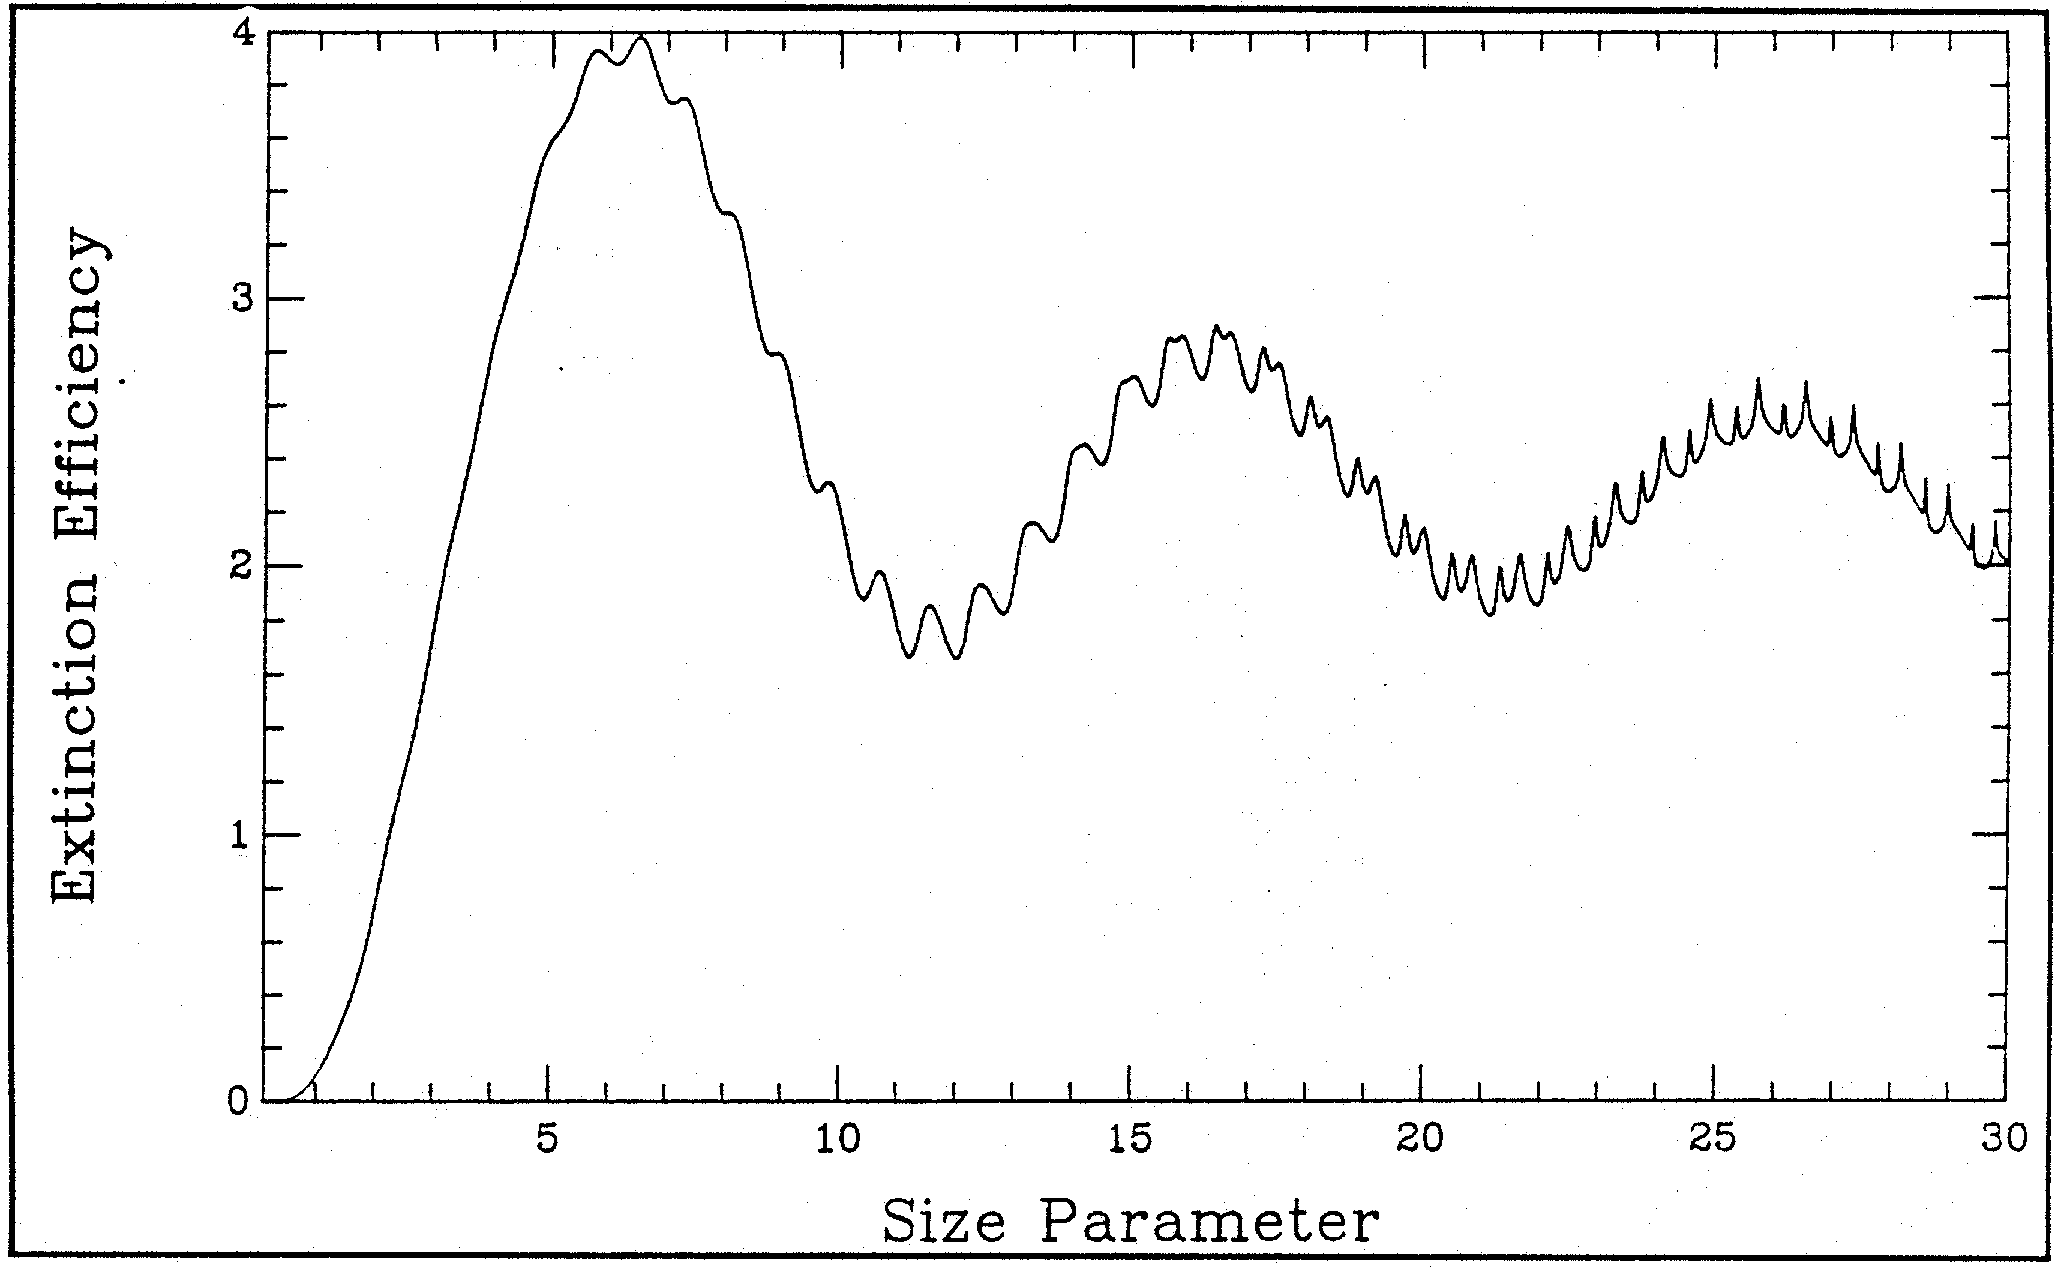
\includegraphics[width=1.0\textwidth]{grainger_ch5_Qext_vs_wavelength.png}
\caption{The variation of $Q_{\textnormal{ext}}$ as a function of the size parameter $\alpha = (2\pi r/\lambda)$ at a fixed value (1.33) of the complex refractive index $m$. Source: http://eodg.atm.ox.ac.uk/user/grainger/research/book/protected/Chapter5.pdf}
\label{Qlambda_curve}
\end{center}
\end{figure}

As mentioned earlier, at wavelengths in and around the optical spectral region, the absorption mechanism in the ISM is dominated by interstellar dust. Typical interstellar dust grains have radii ranging between 100 and 1000 nm \citep{2000JGR...10510299W}, but the dominant grain size is 300 nm \citep{2003JGRA..108.8030L}. Therefore, the condition $\lambda \sim\ r$ is satisfied for interstellar dust in the UV-to-near-IR spectral range, which covers approximately a 100-1000 nm wavelength range. Therefore, $\sigma(\lambda)$ is greatest when the photon wavelength is in the region of 300 nm, which is located within the UV wavelength regime. The effect of extinction is therefore significantly greater in the UV than in the IR. Although this spherical model is somewhat simplistic for the case of interstellar dust grains, its general conclusions align with observational results.\\*

If we refer back to Equations \ref{optical_depth} and \ref{flux_loss_optical_depth}, with this knowledge of the behaviour of $\sigma$, it can be seen that in the UV-to-NIR regime, the optical depth (and hence extinction) is greater at shorter, bluer wavelengths,  which causes the source star to appear redder than its true colour. Hence, the effect of extinction is sometimes referred to as ``reddening''. \\*

\section{Extinction in stars and stellar populations}
All stars emit light from their surfaces, above which the photons can travel much more freely than in the stellar interior. However, the emitted photons must pass through the stellar atmosphere immediately above the surface before reaching the ISM or a distant observer. The stellar atmosphere contains atomic and ionic species which can interact with the photons. The level of interaction between the photons and the atmosphere depends not only on the photons' wavelengths but also on the nature of the atmosphere itself, which is governed by the type of star in question.

\subsection{The effect of extinction on the observed magnitudes of different stellar types} \label{params}

To understand how extinction affects observations of stellar populations, therefore, we must first understand its effects on the observed magnitudes of different stellar types. To do this, we must first define the fundamental parameters that describe a stellar atmosphere, where the observed beam is first emitted by the star. This is important because these parameters will be used in this project as the input variables on which any star-to-star variations in extinction will be modelled. Stellar atmospheres are defined by three stellar parameters: the effective temperature, surface gravity and metallicity.\\*

\subsubsection{Effective temperature}

\begin{figure}[h!]
\begin{center}
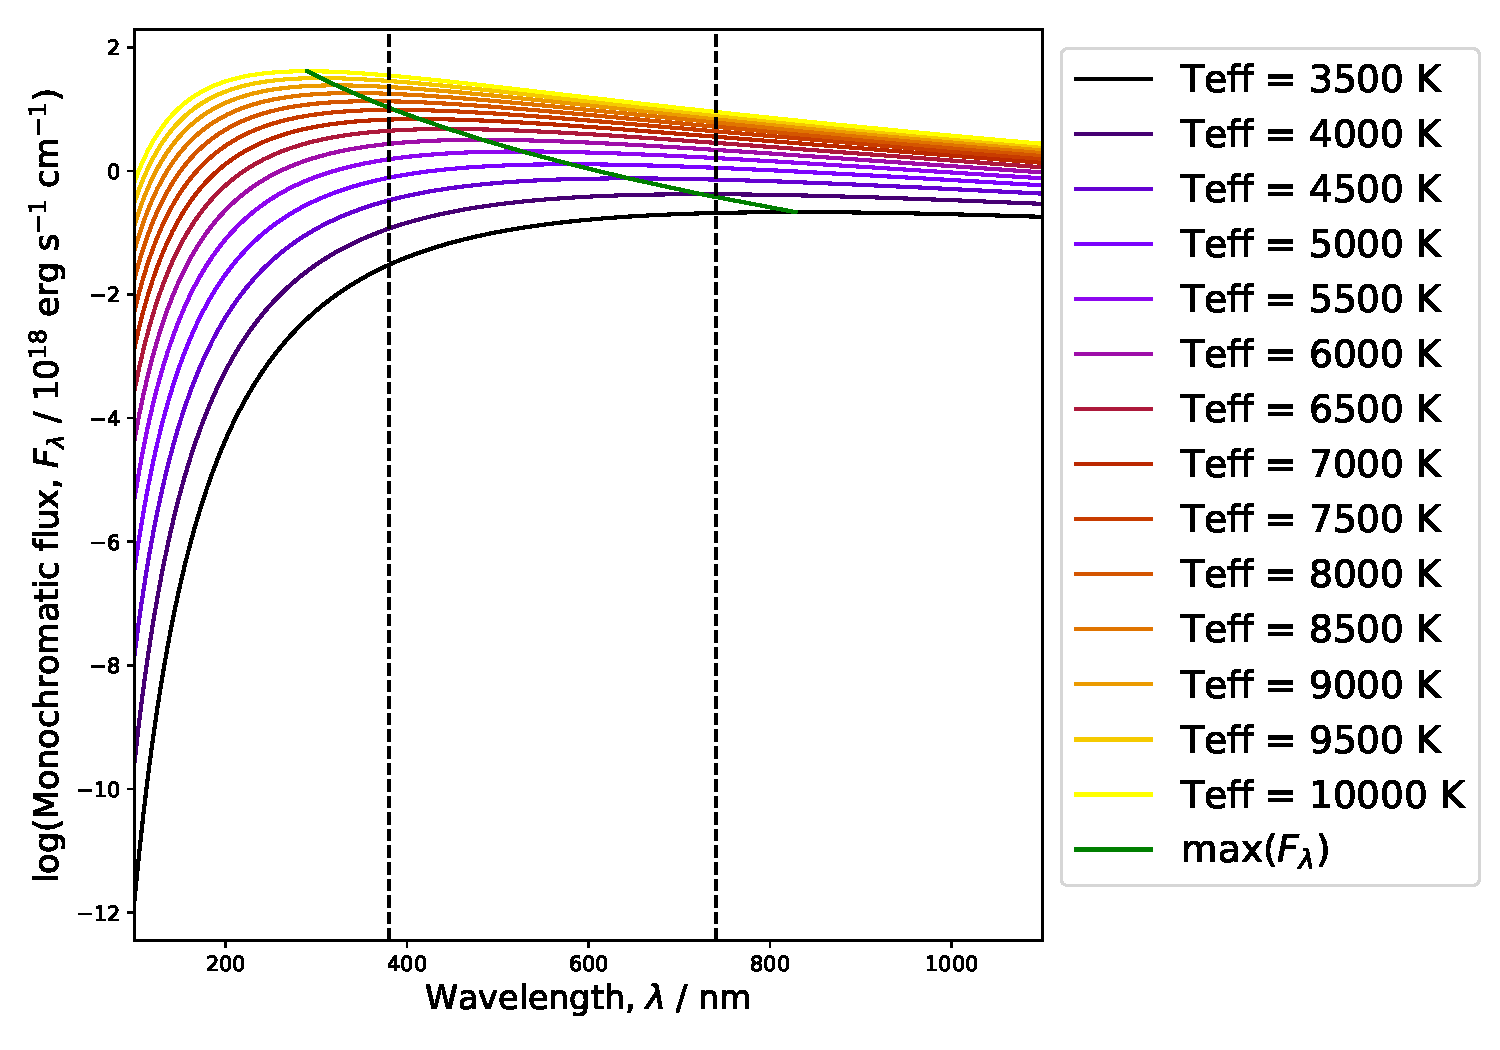
\includegraphics[width=1.0\textwidth]{blackbody_teff_logF_illustration.pdf}
\caption{Plot of the logarithm of monochromatic flux of a black body for different stellar effective temperatures, as a function of wavelength. The black dashed lines mark the approximate limits of the visible part of the EM spectrum. The green curve represents the variation of the Planck Law maxima with effective temperature.}
\label{planck_curve}
\end{center}
\end{figure}

The effective temperature ($T_{\textnormal{eff}}$) of a star is defined as the thermodynamic temperature of a black body which produces the same stellar flux across all wavelengths (known as the bolometric flux) as that produced by the star. The equation of the radiation emitted by a black body produces the body's flux per unit wavelength per unit angular viewing area, $F_{\lambda,bb}$, known as the black body's monochromatic flux. The equation, known as the Planck Law, is as follows:


\begin{equation}
F_{\lambda,bb} = \frac{2hc^{2}}{\lambda^{5}\left(\exp\left({\frac{hc}{\lambda k_{B}T}}\right) - 1\right)}
\label{planck_bb}
\end{equation}
where $T$ is the thermodynamic temperature of the black body, $h$ is Planck's constant, $c$ is the vacuum speed of light and $k_{B}$ is Boltzmann's constant. This equation also holds if the light wave frequency $\nu$ is used instead of the wavelength, with the monochromatic flux $F_{\nu,bb}$ now being the black body flux per unit frequency per unit angular viewing area:

\begin{equation}
F_{\nu,bb} = \frac{2h\nu^{3}}{c^{2}\left(\exp\left({\frac{h\nu}{k_{B}T}}\right) - 1\right)}
\label{planck_bb_freq}
\end{equation}
In this project, the definition of monochromatic flux for any given object will be reserved exclusively for the flux per unit wavelength, $F_{\lambda}$, with any calculations involving black body fluxes using Equation \ref{planck_bb}. \\*

The general approximation of stars to black bodies (and hence the actual stellar surface temperature to $T_{\textnormal{eff}}$) is valid because all stars have been observed to have spectra that closely resemble those of black bodies, with the notable exception of atmospheric absorption lines. The (intrinsic) bolometric luminosity of a star is used to define the effective temperature via:

\begin{equation}
L = 4 \pi R^{2} \sigma_{SB} T_{\textnormal{eff}}^{4}
\label{Teff_def}
\end{equation}
where $R$ is the (mean) stellar radius. Effective temperature has an effect on interstellar extinction due to its strong effect on the stellar luminosity and, hence, the flux, via the Planck Law in Equation \ref{planck_bb}. For a higher effective temperature, as demonstrated in Figure \ref{planck_curve}, there will be more photons in the broad beam of light with wavelengths that make them likely to interact with the local ISM. \\*

\subsubsection{Metallicity}

The atmosphere of any given star always contains a variety of chemical species, depending on the overall composition of the star. These different chemical species each have different orbital configurations of atomic/ionic electron states. An electron in a given state absorbs and emits photons at a particular wavelength, which varies between individual states and between different atoms. Although the light absorbed by an atomic electron is re-radiated, over a large number of electrons this radiation is emitted isotropically, causing a net decrease in the flux travelling out of the stellar atmosphere in the direction of a given observer at that wavelength. Therefore, in a given wavelength range, such as that defining a particular photometric filter, a greater proportion of light in a broadband beam is absorbed in a medium containing a mixture of many different elements than in a medium dominated by one or two elements. The chemical composition of an astrophysical object is quantified by its metallicity.\\*

From observations, it is clear that hydrogen is the most abundant element in stellar atmospheres, with helium a clear-but-distant second. The metallicity of a star is defined as the fractional abundance of heavy elements, often approximated by iron (Fe) alone, relative to the star's hydrogen (H) abundance, compared to that of the Sun. The abundances are determined by the strength of the elements' characteristic absorption lines in the stellar spectra, and the metallicity itself is defined via the following equation:

\begin{equation}
\textnormal{[Fe/H]} = \log\left(\frac{N_{\textnormal{Fe}}}{N_{\textnormal{H}}}\right) - \log\left(\frac{N_{\textnormal{Fe},\odot}}{N_{\textnormal{H},\odot}}\right)
\label{FeH_def}
\end{equation}
where $N_{E}$ represents the number density for a given atomic species $E$. For stellar observations, $N_{E}$ is measured at the stellar surface. Since the output of Equation \ref{FeH_def} is logarithmic, a value of [Fe/H] = 0 indicates solar metallicity. An increase in metallicity would cause the relevant metallic absorption and emission lines to be stronger. An increased [Fe/H] value also implies an increase in abundance of sub-ferrous metals. The presence of more nuclear species, each with unique absorption line configurations, inevitably creates more observable absorption and emission lines. For a given atomic electron transition, the difference in intensity between absorbed and emitted flux corresponds to the difference between the atmospheric temperature in the region at which particles of the species in question are located, which dictates the flux of the emission line, and the effective temperature of the star, which dictates the flux of the underlying continuum \citep{1981ApJS...45..635V}. If the temperature at the particles' location is lower than $T_{\textnormal{eff}}$, the emission produces a lower flux than the flux originally absorbed by the particles. The net result is an absorption line at the relevant photon wavelength for this transition. Conversely, if the local atmospheric temperature is higher than $T_{\textnormal{eff}}$, the emitted flux is higher than the absorbed flux and the overall result is an emission line at the transition photon wavelength. Figure \ref{sun_atmopshere_structure} shows the temperature distribution of the atmosphere of the quiet Sun (i.e., determined at the phase of minimum solar activity) and the approximate atmospheric locations of various species which produce observable emission/absorption features. This illustrates the complexity of determining the overall impact of metallicity, for any stellar atmosphere, due to the importance of local conditions for the species producing each individual spectral feature \citep{1981ApJS...45..635V}, as noted previously.\\*

\begin{figure}[h!]
\begin{center}
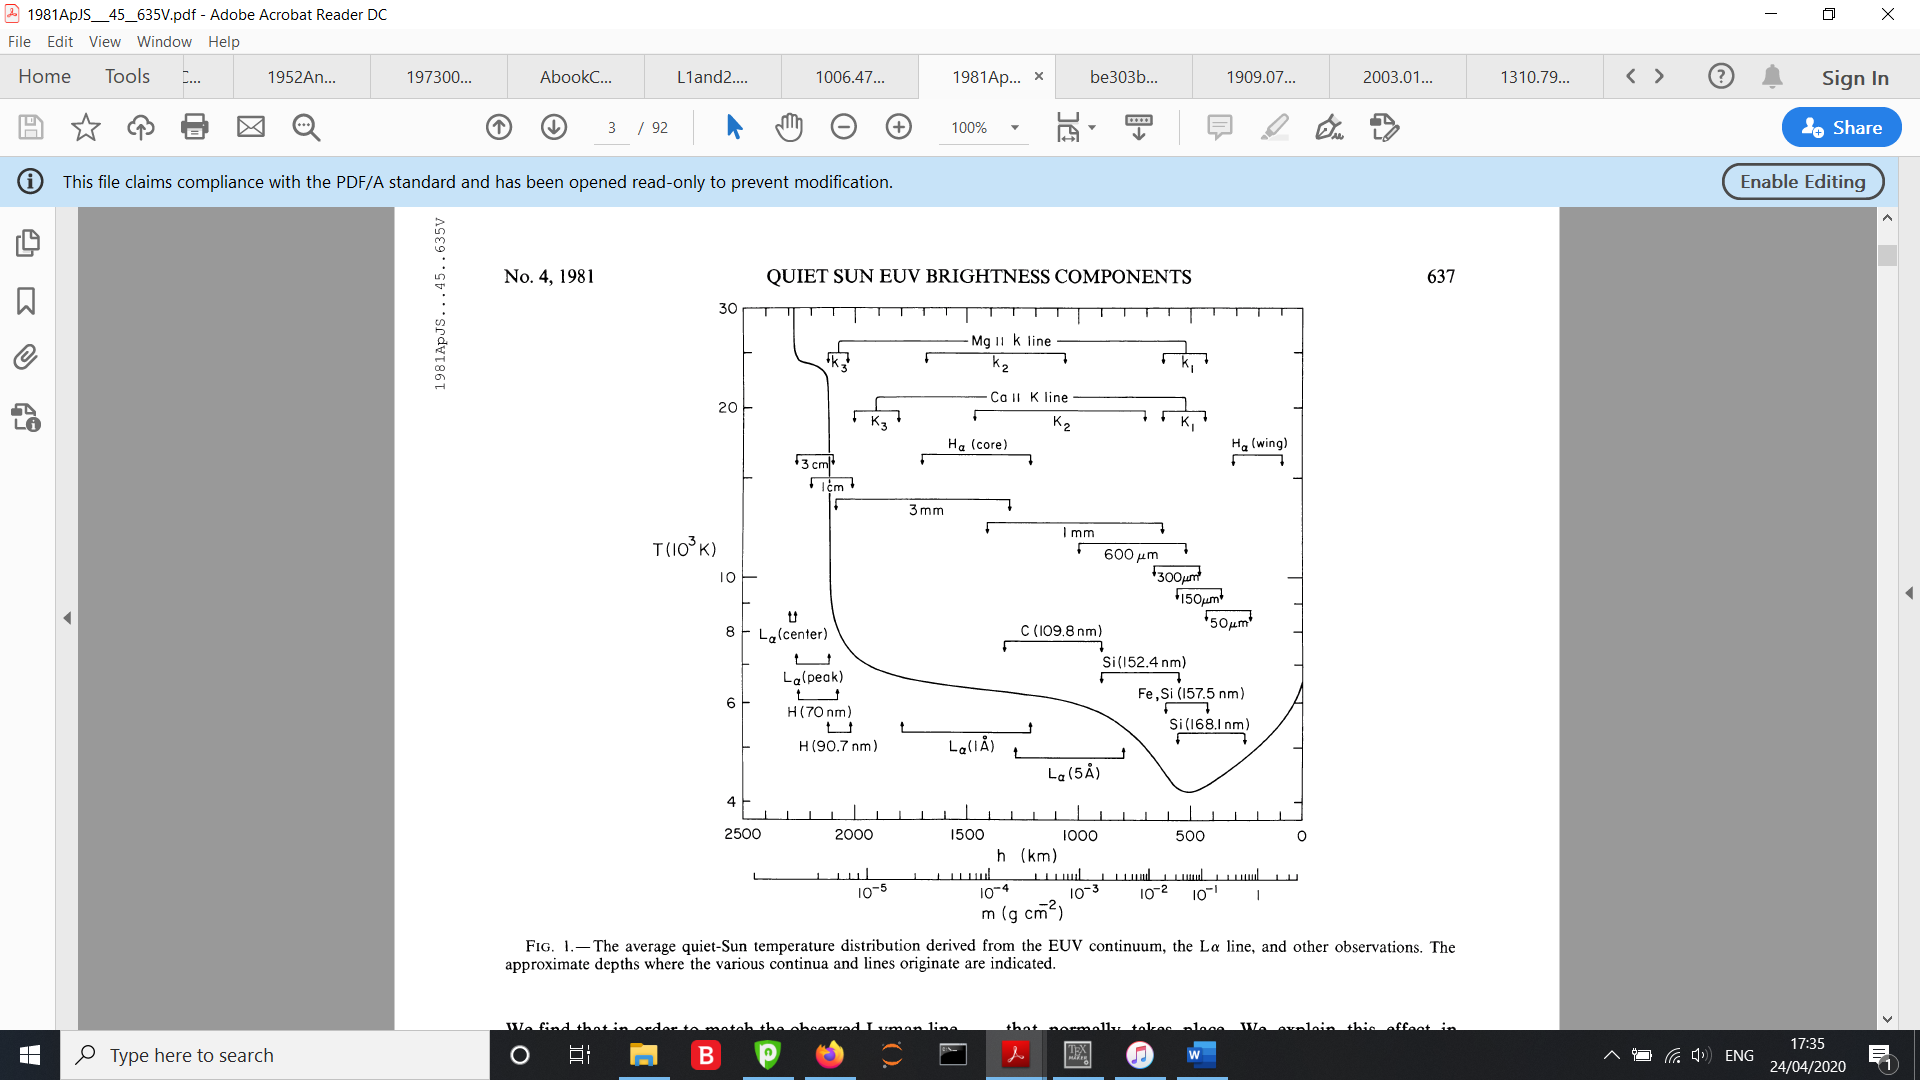
\includegraphics[width=1.0\textwidth]{1981_vernazza_solar_chromosphere_structure.png}
\caption{Empirically-determined average temperature ($T$) as a function of atmospheric height ($h$) and column mass density ($m$) for the atmosphere of the  quiet Sun. For each named line and continuum emission in this plot, the limits for the approximate location of their respective source species is shown. Source: \cite{1981ApJS...45..635V}}
\label{sun_atmopshere_structure}
\end{center}
\end{figure}

In conclusion, therefore, the effect of metallicity on the flux lost or gained by the stellar spectrum in the stellar atmosphere is itself dependent on the thermodynamic properties of the atmosphere and these properties' effect on each individual electron transition. Since these properties are themselves determined by the choice of model atmosphere, the effect of metallicity is unique to each atmosphere and is therefore very difficult to predict for a wide range of stellar atmospheres.\\*


\subsubsection{Surface gravity}

The definition of the stellar surface gravity $g$ is simply the value of the standard Newtonian gravitational acceleration, applied to the stellar surface (the mass is the total stellar mass, $M$, and the distance is the stellar radius, $R$):

\begin{equation}
g = \frac{GM}{R^{2}} = \frac{4\pi G\int_{0}^{R}\rho(r)r^{2}dr}{R^{2}}
\label{gravity_def}
\end{equation}
A greater surface gravity, as can be inferred from Equation \ref{gravity_def}, represents a surface with a higher mass density. For stars, being self-gravitating, this infers a higher atomic number density.  \\*

%the effect of atomic number density on

The effects of surface gravity on the stellar emission spectrum arise directly from the quantum mechanical properties of the interactions between the photons and atomic electrons in the stellar atmosphere. While stellar spectral lines are always broadened due to the Heisenberg uncertainty principle (an effect known as ``natural broadening''), they can be broadened further by additional effects arising from the proximity (i.e. number density) of particles at the stellar surface, which is described by the strength of the stellar surface gravity. \\*

%When a particle, such as an electron, absorbs a photon, the absorption process is not instantaneous and therefore carries an uncertainty in the time taken for the process to be completed, with a corresponding uncertainty in energy due to the Heisenberg uncertainty principle. Across a large number of absorptions for the same initial electron state, the result is a spread in the energies of the absorbed photons. The associated emission line is therefore broadened by the multiple wavelengths of the photons. This is universal and referred to as ``natural broadening''.\\*

The impact of stellar effective temperature, metallicity and surface gravity on extinction arises through their described effect on the observed spectral energy distribution (SED) which leaves the stellar atmosphere. The magnitudes of both this SED and the overall interstellar extinction are functions of wavelength. Between these two quantities, therefore different stellar types, which generate different SEDs, can be impacted to different extents by the overall extinction at a given wavelength. The difference in the extinction for different stellar types can be magnified or diminished depending on the ISM extinction and, therefore, on the wavelength at which the observations are made.

\subsection{Determining properties of stellar populations}
\subsubsection{The role of CMDs} \label{CMDs_intro}
If we compare the individual black body spectra in Figure \ref{planck_curve}, it can be seen that the maximum monochromatic flux of the black body occurs at an increasingly shorter wavelength for objects with increasingly higher temperatures, as indicated by the green curve connecting the $F_{\lambda,bb}$ maxima at different temperatures. This makes a hotter object appear bluer to an observer. The relationship between the wavelength at which the monochromatic flux is maximal ($\lambda_{max}$) and the black body temperature ($T$) is quantified by Wien's displacement law:

\begin{equation}
\lambda_{max} T = 2.898 \times 10^{6} \textnormal{ nm K}
\label{wien_eq}
\end{equation}
More importantly, Figure \ref{planck_curve} demonstrates that, within the UV-to-IR wavelength regime, the change between values of the logarithm of the monochromatic flux at two different wavelengths is always greater for stars with lower effective temperatures. Therefore, to measure a star's effective temperature, observers compare the star's observed flux in two filters operating at different wavelengths within this range. The difference between the star's flux magnitudes in each of the two filters is then taken, with the magnitude for the redder filter being deducted from that of the bluer filter. This quantity is known as the colour index. For two filters $X$ and $Y$, with $X$ being bluer than $Y$, the colour index of observations made using those filters, $(X-Y)$, is defined as:

\begin{align}
\begin{split}
(X-Y) &= m_{X} - m_{Y} \\
 &= (m_{X,0} - m_{Y,0}) + (A_{X} - A_{Y}) \\
 &= (X-Y)_{0} + E_{X-Y}
\end{split}
\label{colour_index}
\end{align}
where $(X-Y)_{0}$ is the true or intrinsic colour index of the object, $m_{X,0}$ and $m_{Y,0}$ are the object's intrinsic apparent magnitudes in $X$ and $Y$, respectively, and $E_{X-Y} = A_{X} - A_{Y}$ is known as the colour excess, but can also be denoted in literature using the term ``reddening''. The colour excess represents the effect of extinction on the observed colour index. Its importance arises from the prominence of the intrinsic colour index in determining effective temperature. Higher values of $(X-Y)$ indicate redder stars, with lower effective temperatures, as shown in Figure \ref{planck_curve}. The greatest advantage of using a colour index is that, because it is defined as the difference between two magnitude measurements, it is independent of the source's distance from the observer.\\*

The most commonly-used colour index, employed as a reference for most optical observations, is the Johnson ($B-V$) index. These filters are part of the Johnson-Morgan UBV filter system (often simply known as the Johnson system) \citep{1953ApJ...117..313J}, later extended as the Johnson-Cousins UBVRI \citep{1990PASP..102.1181B} system, which has been widely used and highly studied for decades and continues to be the standard reference for more modern filter systems. The Johnson blue ($B$) and yellow ($V$) filters which define the ($B-V$) colour index are of particular importance, as these formed the original benchmark for observing stellar populations and evolutionary stages. Using this filter system as a reference also allows for better comparisons of data from different instruments, including data from older archives.\\*

It can be seen from Equation \ref{Teff_def} that the luminosity (and therefore flux) of a star is dependent on radius as well as effective temperature. If a plot is made of luminosity against effective temperature (known as a Hertzsprung-Russell or HR diagram), it can be seen that all stars in a given star cluster follow a single, complex track. Because the stars are approximately the same age in a typical cluster population, this track is known as an isochrone. Isochrones for different population ages and metallicities are calculated using theoretical stellar models, which cover the largest possible spread of initial stellar masses for the required age.\\*

By examining Equations \ref{ext_def_app_mag} and \ref{colour_index}, it becomes clear that both the absolute filter magnitudes and the intrinsic colour indices can be combined with information from theoretical stellar evolution models to calculate the bolometric stellar luminosity $L$ from observational flux data. To determine the detailed properties of stellar populations, all stars in an observational sample or star cluster are plotted together on a pair of axes known as a colour-magnitude diagram (CMD), which represents an observational analogue of the HR diagram \citep{2005ARA&A..43..293B}. The absolute magnitude of stars in a given filter $Z$, $M_{Z}$, is on the vertical axis, with the flux increasing (and the magnitude value decreasing) upwards. The intrinsic colour index of the stars in two filters $X$ and $Y$, $(X-Y)_{0}$, is on the x-axis, with the values increasing (and stars becoming redder) to the right. Note that filter $Z$ may be the same as either $X$ or $Y$.\\*

In practice, the universal general shape and position of stellar populations in the HR diagram and each observational CMD, particularly the position and shape of the stellar main sequence, provides a highly useful tool for comparing stellar populations with unknown distances and extinction values to known examples and to theoretical models. This is done by alignment of the respective main sequences in CMDs, particularly the upper main sequence below the MSTO position, which contains the most luminous MS stars and is less sensitive to the (initially unknown) value of the cluster metallicity than the lower MS. \\*

The age of an observed stellar population is determined by, firstly, correcting the data for the effects of distance and extinction and, secondly, aligning a series of isochrones, each of a different age, with the main-sequence (MS) of the observed data. The accepted age of the population is that of the isochrone which most closely follows the progression of stars along the main-sequence turn-off (MSTO). As such, any errors in the estimated extinction can potentially change the age of the best-fit isochrone and therefore produce an erroneous estimate of the true population age. This project will examine the effect of potential errors in the calculation of extinction in stellar populations.

\subsubsection{Comparing theoretical and observational quantities} \label{add_ext}
For any observational dataset of stars, the stars' individual extinction values will be completely unknown from the data alone. In order to compare observational and theoretical data, the most convenient approach is to add the (theoretical) extinction values to the theoretical dataset magnitudes (i.e., absolute magnitudes), before comparing to the distance-corrected observational data. As a result, the quantity from each dataset that is being compared is the absolute magnitude plus the extinction in each filter. If we label this quantity $M_{\textnormal{ext},X}$ for a generic filter $X$, we can define it as:

\begin{equation}
M_{\textnormal{ext},X} = M_{X} + A_{X}
\label{MextX_def}
\end{equation}
Using Equation \ref{ext_def_app_mag}, Equation \ref{MextX_def} can now be rewritten such that $M_{\textnormal{ext},X}$ can be defined using both quantities derived directly from observations and those determined by theoretical models:

\begin{align}
\begin{split}
M_{\textnormal{ext},X} &= M_{X} + A_{X} \textnormal{ (theoretical data)}\\
 &= m_{X} + 5 - 5\log\left(\frac{d}{\textnormal{pc}}\right) \textnormal{ (observational data)}
\end{split}
\label{MextX_eq}
\end{align}
This allows for direct comparison of theoretical data, whose stars are treated with theoretically-determined $A_{X}$ values, with distance-corrected observational data, whose stars have unknown $A_{X}$ values. Equation \ref{MextX_eq} therefore provides a pathway for comparing the standard treatment of extinction (constant $A_{X}/A_{V}$ ratios) with the treatment proposed in this project ($A_{X}/A_{V}$ varying as functions of intrinsic stellar parameters). To calculate colour indices for stars in the isochrones, the difference between $M_{\textnormal{ext}}$ values in two filters, $M_{\textnormal{ext},X} - M_{\textnormal{ext},Y}$, is simply equal to the observed colour index $(X-Y)$, as shown by Equation \ref{colour_index}.\\*

In practice, therefore, due to the unknown extinction values for the individual stars and the cluster as a whole, the axis parameters for the generic CMD described in Section \ref{CMDs_intro} are $M_{\textnormal{ext},Z}$ and $(X-Y)$, via Equation \ref{colour_index}, instead of $M_{Z}$ and $(X-Y)_{0}$, respectively.\\*

\section{Empirical extinction curves} \label{empirical}

From the results of Mie scattering summarised in Section \ref{ext_def}, it is clearly very important to both understand and measure any variations in extinction. In fact, the observed variation of extinction with wavelength discussed in the previous section has been studied for decades. Various authors have produced empirical results intended to better model the changes in the magnitude of extinction over an extended wavelength range, as explicit functions of wavelength or as values or functions unique to each one of a selection of photometric filters.\\*

%Johnson-Cousins filters , which have long been the standard set of filters in UV-IR spectral observations, 

\cite{1985ApJ...288..618R} found that outside dense molecular clouds, which have high opacities and whose lines-of-sight are less frequently used in observations as a result, all extinction laws for all the filters they studied were uniform between wavelengths of 1 and 13 $\mu$m when observing sources in the direction of the Galactic Centre. This result was then used to produce constant ratios of the extinction in those filters ($A_{X}$, where $X$ represents a generic photometric filter) to the extinction in the Johnson $V$ filter ($A_{V}$). The ratio between the extinction in $X$ and that in $V$ is denoted by $A_{X}/A_{V}$. They also determined the now-widely used global average value of 3.08 ($\sim$3.1) for $R_{V} \equiv A_{V}/E_{B-V}$, known as the total-to-selective extinction ratio,  for the diffuse ISM. \\*

\cite{1989ApJ...345..245C} used observations of mostly bright, hot O- and B-type main-sequence stars to produce empirical equations describing the mean ratio of extinction values at a specific wavelength $\lambda$ ($A_{\lambda}$) to the $V$-band extinction ($A_{V}$), this ratio being denoted $A_{\lambda}/A_{V}$. The study produced a basic equation of the form:

\begin{equation}
A_{\lambda}/A_{V} = a(x) + b(x)/R_{V},
\label{CCM_general}
\end{equation}
where $x \equiv 1/\lambda$. The significance of $R_{V}$, as noted in the same paper, comes from its usefulness as an indicator of the nature of the interstellar medium through which the observed light travels in order to reach the observer. The total wavelength range was divided into 4 sub-ranges, each with a governing pair of empirically-determined equations to calculate $a(x)$ and $b(x)$, respectively. The extinction-ratio profiles calculated using Equation \ref{CCM_general} for three lines of sight are displayed in Figure \ref{cardelli_curve}.\\*

\begin{figure}[h!]
\begin{center}
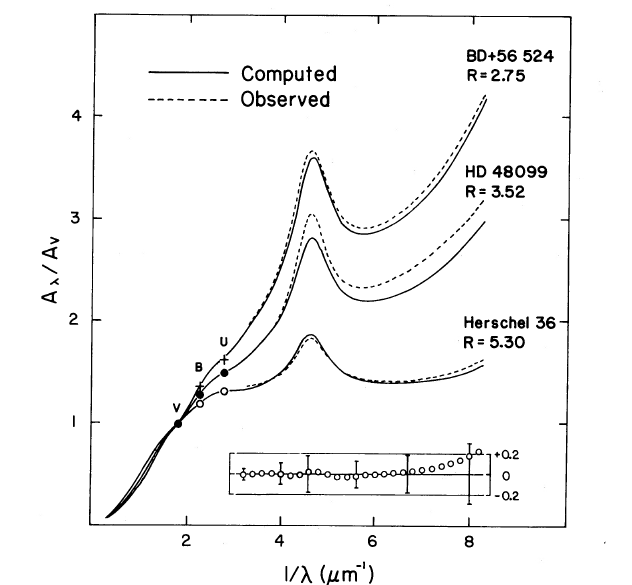
\includegraphics[width=1.0\textwidth]{cardelli_curve_fig4_crop.png}
\caption{Variation of the extinction, normalised to the $V$-band extinction $A_{V}$, as a function of wavelength, in spectral regions ranging from the IR (left) to the UV (right). The solid lines are calculated using Equation \ref{CCM_general} at the given $R_{V}$ values. These values represent the lines of sight for their respective source stars, which are listed alongside.  Source: \cite{1989ApJ...345..245C}}
\label{cardelli_curve}
\end{center}
\end{figure}

This model underpins more recent studies of intrinsic effects on extinction \citep{2008PASP..120..583G,2014MNRAS.444..392C,2018MNRAS.475.5023C,2018MNRAS.479L.102C}, and provides the basis for the synthetic $A_{X}/A_{V}$ datasets in this project. Equation \ref{CCM_general} has become a standard model for theoretical studies to employ for predictions made in the UV, optical and near-IR wavelength regions, although it is not always accurate \citep{1994ApJ...422..158O,1999PASP..111...63F}. \\*

\cite{1994ApJ...422..158O} found deviations from the \cite{1989ApJ...345..245C} extinction law in the soft-UV spectral range using a sub-sample of 22 stars from the same dataset. This was attributed to the uncertainty in the short-wavelength cutoff of the UV-range Johnson $U$ filter and to the presence of the Balmer discontinuity within the limits of the filter bandpass.\\*

For broadband filters, the filters' wavelength ranges are large enough such that the spectral variations the stellar flux with wavelength can be significant within these ranges. This can cause errors when estimating the true stellar flux in a broadband filter, as the filter's effective wavelength can change significantly between different stars, even after accounting for all other observational factors. The issue of effective wavelengths will be described in more detail in Section \ref{colour_corr} later. Because of this issue, due to the broadband nature of the Johnson filters and the general decrease of extinction with increasing wavelength, \cite{1999PASP..111...63F} found that the \cite{1989ApJ...345..245C} relations overestimate the extinction in the near-IR and blue-visible Johnson filters. The study put forward corrections to the equations for $a(x)$ and $b(x)$ for these wavelength regions. However, in the UV region covered by the \cite{1989ApJ...345..245C} equations, \cite{2004ApJ...616..912V} found the equations to be accurate for 93\% of a homogeneous UV observational database.\\*

\cite{2014MNRAS.444..392C,2018MNRAS.475.5023C,2018MNRAS.479L.102C}, using bolometric corrections (which will be described in Section \ref{bol_corr}), created simple  models for the parameter $R_{X}  = (A_{X}/E_{B-V})$, consisting of a quadratic variation with effective temperature and a linear variation with metallicity (they found no significant variations with surface gravity) in multiple telescope filter systems. This was based on MARCS model stellar atmospheres, which have an upper effective temperature limit of 8000K \citep{2008A&A...486..951G}. The equation is independent of surface gravity and has the following form:

\begin{equation}
R_{X} = a_{0} + T_{4}(a_{1} + a_{2}T_{4}) + a_{3}\textnormal{[Fe/H]}
\label{casagrande_ext_fit}
\end{equation}
where $T_{4} = 10^{-4} \times T_{\textnormal{eff}}$ and $T_{\textnormal{eff}}$ is the effective temperature. The equation is valid for $5250\textnormal{K} \leq T_{\textnormal{eff}} \leq 7000\textnormal{K}$. Although these models are mathematically simple (with only 4 coefficients), the limited $T_{\textnormal{eff}}$ range in which they are applicable is problematic, particularly in the red giant branch (RGB) and lower main sequence of any stellar population.\\*

\section{The standard treatment of extinction in observed stellar populations} \label{standard_ext}

In observations, the extinction for a given source is initially unknown. For a stellar population, observers must make use of distinctive features of stellar populations that can be used as standard candles to estimate the distance to the population independently from extinction effects, allowing the extinction to then be calculated separately. Even after distance effects are removed from the data, however, the extinction in a stellar population is not trivial to calculate. In practice, the standard approach is for observers to use fixed values for the extinction ratio $A_{X}/A_{V}$ in each filter. These fixed values are often taken from \cite{1985ApJ...288..618R} or calculated using the \cite{1989ApJ...345..245C} law for the filters' central wavelengths \citep{2018ApJ...868...25B,2020A&A...633A..38D}, which will be explained in detail in Section \ref{filter_desc}. Examples of constant filter. This approach has the issue of assuming that $A_{X}/A_{V}$ is constant for all stars in a given stellar population, meaning the fraction of flux lost between the stellar surface and the observer for any beam in the wavelength range of $X$ is always directly proportional to the fraction lost in the $V$ band for all stars. This results in  $A_{X}/A_{V}$ values that do not account for variations between spectra of different stellar classes, which is shown to be inaccurate by the results of \cite{2008PASP..120..583G} and by the data shown in Figures \ref{just_data_FeH0_WFC3gaia} and \ref{just_data_FeH0_ACS} in Section \ref{ext_ratio_data}.\\*

\cite{2008PASP..120..583G} produced data tables of $A_{X}/A_{V}$ for stellar atmosphere models with parameters $T_{\textnormal{eff}}$, log($g$) and [Fe/H]. They carried this out using the same ATLAS9 data \citep{2004astro.ph..5087C} that was used to generate the data for this project, but also combined it with data from other studies, which are listed in \cite{2002A&A...391..195G}, resulting in data covering a parameter space extending beyond the ATLAS9 limits in all three parameters. They used the data tables to calculate the $A_{X}/A_{V}$ values for the stellar models in Padova theoretical isochrones \citep{1994A&AS..106..275B}. While determining that the values of $A_{X}/A_{V}$ varied significantly with $T_{\textnormal{eff}}$ and log($g$), the variation with metallicity was found to be $\sim$0.17$\%$ between [Fe/H] = 0.0 and [Fe/H] = -2.5. They found that, when they set $A_{V} = 6$, there was a systematic shift for the ACS filter system between extinction values calculated star-wise using the tables of $A_{X}/A_{V}$ data and a constant extinction value applied to the entire isochrone. The constant values of $A_{X}/A_{V}$ were calculated from a yellow dwarf in the low-extinction regime. Overall, in the single ACS CMD example shown in the study, the $A_{X}/A_{V}$ tables produced a smaller extinction value in the F814W filter and a larger (F475W-F814W) colour index value. It also caused a change in the shape of the curve at the main-sequence turn-off (MSTO) point. They then applied the data from the tables to the case of the globular cluster M92. They found the optimal metallicity to be $Z = 0.0004$ ([Fe/H] $\approx$ -1.6) instead of the value obtain by previous observers of $Z = 0.0001$ ([Fe/H] $\approx$ -2.2). Therefore, their use of $A_{X}/A_{V}$ data caused the estimated cluster metallicity to be greater than when using the standard one-size-fits-all approach to extinction.\\*

\cite{2017Galax...5...28O} used the tabulated extinction ratio tables resulting from \cite{2008PASP..120..583G}, which demonstrated the effect of stellar parameters on the calculated extinction ratios, to search for potential discrepancies in the predicted ages of isochrones after the addition of extinction. This was performed for isochrones with real ages between 12 and 13 Gyr and employed a small selection of Johnson ($B$,$V$ and $I$) and ACS (F606W, F775W and F814W) broadband filters. They found that, by employing the \cite{2008PASP..120..583G} data, the position of a given isochrone in the CMD shifted such that, at $A_{V} = 1$, the position of the MSTO of a 12 Gyr isochrone with individual stellar extinction values added is the same as the MSTO position for a 12.5 Gyr isochrone with the standard fixed extinction value added.\\*

\section{Project objectives}
The first goal of this project is to investigate the variations of the extinction ratios $A_{X}/A_{V}$ in selected photometric filters within multiple filter systems with changes in effective temperature, surface gravity and metallicity. This will be carried out using a large library of theoretical stellar spectra covering all main stages of stellar evolution. Analytic fitting functions will be employed to model the $A_{X}/A_{V}$ variations in each filter as a function of the stellar parameters. \\*

The results of the fitting process will then be applied to the CMD of a representative observational example of a relatively high-extinction open cluster. The CMD will be fitted with two theoretical isochrones. For the first case, a constant $A_{X}/A_{V}$ value will be applied to the entire isochrone. For the second, varying $A_{X}/A_{V}$ values will be applied, using the fitting results. The best estimates for the ages, metallicities and $A_{V}$ values in both cases will be compared, giving a quantitative illustration of the importance of the effect of the stellar parameters on $A_{X}/A_{V}$ ratios used in CMD fitting.\\*



\chapter{Data \& methodology}
In this chapter, the method used for calculating photometric filter-based extinction ratios will be described, including relevant formulae and choices of input parameters. The filters used in this project will be listed together with their basic properties. The variations shown in the extinction ratio data caused by changes in the stellar atmosphere parameters will be described, together with a brief overview of the process used to determine and fit the appropriate mathematical models of these variations. The process by which the resulting extinction ratio models are applied to theoretical isochrones is described and the resulting isochrones are then compared to isochrones produced using the standard fixed-extinction approach summarised in Section \ref{standard_ext}. The final step in the methodology is to demonstrate the effect of using different extinction-calculation methods on an observed stellar population. The data for the selected cluster and the results of previous observational studies for the cluster are described. Selection criteria used to improve the quality of the observed dataset are introduced and employed, with the results shown. The choice of criteria made for the final dataset chosen to be analysed is stated and justified and the method used for fitting the isochrones to the dataset and comparing the results of using different extinction-calculation methods is summarised.\\*

Finally, a brief overview is given of the software used for this project, including summaries of the theoretical models used in this project to generate isochrone and stellar atmosphere data and the software created in this project to analyse the data and produce the numerical and graphical results that form the bases of the conclusions made in this project.

\section{Calculating extinction ratio data} \label{ext_ratio_data}

When observing stars through a photometric filter, only a small fraction of the bolometric stellar flux that reaches the telescope is detected, since stars emit photons with wavelengths across the full EM spectrum. This is due to the design of the filter in question, which determines the fraction of photons detected at a given wavelength, known as the transmittance. The variation in transmittance as a function of photon wavelength is known as a transmission curve, bandpass or filter response function. The range of wavelengths for which the transmittance is non-zero, for any filter, is very narrow when compared to the full EM spectral range.\\* 

The significance of this relatively narrow wavelength range occurs when analysing observational data using the results of theoretical stellar models, which determine the state of a stellar evolution model at a specified age, in the form of isochrones. In this project, isochrones are the central tool to compare the effects of using variable and fixed extinction ratios on the estimated age of star clusters. The results of theoretical evolutionary models are expressed in terms of a star's bolometric quantities, such as the bolometric luminosity, the effective temperature and the metallicity, which in turn can be used to calculate further important quantities, such as the stellar radius (via Equation \ref{Teff_def}) and surface gravity (via Equation \ref{gravity_def}). Therefore, to correctly compare theoretical models and isochrones (which use bolometric data) to observational photometric data (by necessity limited by the use of filters), mathematical methods must be used to transform the theoretical stellar evolution model data into the form of filter-based fluxes and magnitudes.\\*

\subsection{The role of stellar evolution and atmosphere models}
The first step in this transformation is to compute theoretical stellar spectra. This is done using stellar atmosphere models, which use values of $T_{\textnormal{eff}}$, log($g$) and [Fe/H], taken from the appropriate stellar evolution models, as a basis to produce a theoretical emission spectrum for that star, in the form of a table showing a list of desired wavelengths $\lambda$ and the theoretical monochromatic flux at that wavelength, $F_{\lambda}$, defined at the atmospheric/stellar radius, $R$. To apply the spectrum to the case of a distant observer, the equation linking the relevant flux definitions to the observer distance, $d$, must be included:

\begin{equation}
f_{\lambda}d^{2}=F_{\lambda}R^{2}
\label{flux_dist_rd}
\end{equation}
where $f_{\lambda}$ represents the (theoretical) monochromatic flux at a given wavelength $\lambda$ at the observer's distance from the source. However, as with all flux magnitudes, the predicted apparent magnitude for a distant star, with unknown extinction, must be linked to a known reference point. This requires the detailed knowledge of a reference spectrum, of a nearby star which is unlikely to experience significant extinction. For all filter systems studied in this project, the nearby bright star Vega ($\alpha$ Lyr) was used as the reference object. Using Vega as the reference star is the most well-known approach to photometric calibration \citep{2014MNRAS.444..392C}, not only due to its high apparent brightness and close proximity to Earth, but also due to its spectral classification as an A0 star, which should theoretically have an apparent magnitude $m_{X} = 0$ in any given filter \citep{1953ApJ...117..313J}.\\*

The wavelength range of a generic filter $X$ is defined as increasing from the shortest ($\lambda_{1}$) to the longest ($\lambda_{2}$) wavelength for which its response function is non-zero. After accounting for the effect of interstellar extinction on an object's detected flux, its apparent magnitude in $X$ can be calculated in terms of parameters determine theoretically by both stellar evolution and atmosphere models:

\begin{equation}
m_{X} = -2.5 \log_{10} \left(\frac{ \int_{\lambda_{1}}^{\lambda_{2}} f_{\lambda} \left( 10^{-0.4 A_{\lambda}} \right) S_{\lambda,X} d\lambda }{ \int_{\lambda_{1}}^{\lambda_{2}} f_{\lambda}^{0} S_{\lambda,X} d\lambda }\right) + m_{X}^{0}
\label{app_mag_def}
\end{equation}
where $A_{\lambda}$ is the extinction as a function of wavelength, $S_{\lambda,X}$ represents the filter response function of $X$ and $f_{\lambda}^{0}$ and $m_{X}^{0}$ represent the monochromatic flux and apparent magnitude, respectively, in $X$ of Vega. The use of these two well-determined observational parameters allows the remaining terms to be fixed to a known scale.\\*

\subsection{Bolometric corrections} \label{bol_corr}

For an observed star at an unknown distance $d$, Equation \ref{flux_dist_rd} cannot give the magnitude of the theoretical spectrum at the observer distance, $f_{\lambda}$ with any reasonable certainty. The uncertainty in $f_{\lambda}$ then causes uncertainty regarding the extinction $A_{\lambda}$ given its position in the same integrand in Equation \ref{app_mag_def}.\\*

Stellar evolution models, such as the BaSTI model used in this project, offer predictions for the values of bolometric stellar parameters for as many stellar models as possible, whose results are stored in databases. These parameters include the stellar bolometric luminosity, effective temperature, radius and surface isotope abundances, al of which are relevant to this project. These evolution models are, therefore, very useful, both as a basis from which to begin calculating model stellar atmospheres and for generating isochrones, meaning they are very useful for studying star clusters, whose members are generally born around the same time. However, the bolometric stellar properties generated by the evolutionary models are not described as functions of wavelength, making them useless for the integration terms in Equation \ref{flux_dist_rd}. Equation \ref{flux_dist_rd} does, however, have great value via the inclusion of the well-constrained observed Vega quantities, which provide a necessary reference for interpreting newly-observed stars. Therefore, the uncertainty arising from $f_{\lambda}$ must be eliminated by linking predicted quantities from stellar evolution models to observed quantities. The bolometric data from the models must be converted into filter-based quantities in order to compare theoretical predictions with observational data \citep{1996ApJ...469..355F}, thereby supplying information about the observed stars that cannot be determined from the observations alone \citep{2002A&A...391..195G} and allowing predictions to be made about those stars. The bolometric correction is the quantity which determines this conversion.\\*
To make use of bolometric corrections, the absolute magnitude $M_{X}$ of the star in filter $X$ must be calculated. This can be done using the apparent magnitude $m_{X}$ and the standard equation which links the two quantities:

\begin{equation}
M_{X} = m_{X} - 2.5 \log_{10}\left( \left( \frac{d}{10 \textnormal{pc}} \right)^{2} \right)
\label{abs_mag_def}
\end{equation}
This represents the second step required for the comparison of theoretical isochrones to observational data, and requires the calculation of bolometric corrections. To derive the final equation linking a bolometric correction with the extinction, we start with the definition of a bolometric correction for filter $X$, which is denoted by $BC_{X}$:

\begin{equation}
BC_{X} \equiv M_{\textnormal{bol}} - M_{X}
\label{BC_def}
\end{equation}
where $M_{\textnormal{bol}}$ is its (predicted) absolute bolometric magnitude, defined using:

\begin{equation}
M_{\textnormal{bol}} = M_{\textnormal{bol},\odot} - 2.5 \log_{10} \left( \frac{4\pi R^{2}F_{\textnormal{bol}}}{L_{\odot}} \right)
\label{mbol_sun}
\end{equation}
where $M_{\textnormal{bol},\odot}$ is the solar absolute bolometric magnitude, which is assumed in this work to have a value of 4.75, $L_{\odot}$ is the solar luminosity and $F_{\textnormal{bol}}$ is the bolometric flux at the stellar surface. It should be noted that $F_{\textnormal{bol}} = \sigma_{\textnormal{SB}} T_{\textnormal{eff}}^{4}$ and therefore $4\pi R^{2}F_{\textnormal{bol}}$ is simply equal to the bolometric stellar luminosity $L$, and is therefore determined solely by the theoretical stellar model used. The bolometric correction for filter $X$ can therefore be expressed, via Equations \ref{flux_dist_rd}-\ref{mbol_sun}, purely in terms of extinction, theoretical stellar quantities independent of distance and observationally well-constrained reference parameters:

\begin{align}
\begin{split}
BC_{X} &= M_{\textnormal{bol},\odot} - m_{X}^{0} - 2.5 \log_{10} \left( \frac{4\pi R^{2}F_{\textnormal{bol}}}{L_{\odot}} \right) \\
&+ 2.5 \log_{10} \left( \frac{\int_{\lambda_{1}}^{\lambda_{2}} F_{\lambda} \left( 10^{-0.4 A_{\lambda}} \right) S_{\lambda,X} d\lambda}{\int_{\lambda_{1}}^{\lambda_{2}} f_{\lambda}^{0} S_{\lambda,X} d\lambda} \right)
\label{BC_extinc}
\end{split}
\end{align}
The output value of Equation \ref{BC_extinc} therefore varies with changes in the effective temperature, surface gravity and metallicity of the stellar atmosphere model, via $R$, $F_{\lambda}$ and $F_{bol}$, and the extinction $A_{\lambda}$. $A_{\lambda}$ is usually normalised relative to the extinction in the well-studied Johnson-$V$ filter, $A_{V}$. To extract the value of $A_{\lambda}$, the simple relation

\begin{equation}
A_{\lambda} = \left( \frac{A_{\lambda}}{A_{V}} \right) A_{V}
\label{ratio_eq}
\end{equation}
is used, together with the \cite{1989ApJ...345..245C} extinction law for $A_{\lambda}/A_{V}$, which is monochromatic and therefore must be placed within the integrand of Equation \ref{BC_extinc}. Given that the \cite{1989ApJ...345..245C} extinction law is normalised to $A_{V}$, the value of $A_{V}$ must be specified prior to the calculation of the bolometric correction. Equation \ref{BC_extinc} was implemented twice, once for each of two distinct $A_{V}$ values (for this project these were $A_{V} = 0$ and $A_{V} = 1$). It should be noted that $BC_{X}(A_{V}=0)$ essentially assumes no extinction in any filter. Therefore, two output values were calculated for Equation \ref{BC_extinc}, one for each $A_{V}$ value. The difference between these two outputs was then taken to extract the extinction ratio $A_{X}/A_{V}$, via the following equation \citep{2008PASP..120..583G,2014MNRAS.444..392C}:

\begin{align}
\begin{split}
\left(A_{X}/A_{V}\right)A_{V} &= BC_{X}(0) - BC_{X}(A_{V}) \equiv m_{X,0} - m_{X}(A_{V})
\label{BCs_diff}
\end{split}
\end{align}
%\\ &\approx \left(A_{X}/A_{V}\right)A_{V}
Any dependence of the $A_{X}/A_{V}$ data on the measurements for Vega or the Sun from Equation \ref{BC_extinc} is eliminated during the subtraction, as these terms are unaffected by the $A_{\lambda}$ value. However, effects due to the nature of the atmosphere of the stellar source on the extinction ratio will remain present, in the form of the integrations of $F_{\lambda}S_{\lambda,X}$ and $F_{\lambda}S_{\lambda,X} \times \left( 10^{-0.4 A_{\lambda}} \right)$, respectively, in the two bolometric correction terms in Equation \ref{BCs_diff}. \\*

\subsubsection{The difference between bolometric and colour corrections} \label{colour_corr}
It is important to note that a bolometric correction is different from the equally well-known quantity known as a colour correction. Colour corrections are tools used to determine the true apparent magnitudes and colours of stars which are observed through a particular set of filters, starting from the magnitudes and colours recorded by an instrument using those filters. Observations made using a particular filter are described using the filter's effective wavelength $\lambda_{\textnormal{eff}}$, defined as an average over the filter wavelength interval, weighted by the source spectrum and the filter response function:

\begin{equation}
\lambda_{\textnormal{eff}} = \frac{ \int_{\lambda_{1}}^{\lambda_{2}} \lambda f_{\lambda} S_{\lambda,X} d\lambda }{ \int_{\lambda_{1}}^{\lambda_{2}} f_{\lambda} S_{\lambda,X} d\lambda }
\label{eff_wavelength_def}
\end{equation}
where all terms take the same definitions as in Equation \ref{app_mag_def}. However, with the source stellar spectrum initially unknown, in practice the observed stellar spectrum is calculated using a single fixed wavelength value for the whole filter, known as the reference wavelength, $\lambda_{\textnormal{ref}}$ \citep{2006A&A...447..769P}, instead of the effective wavelength. This does not match with the definition of $\lambda_{\textnormal{eff}}$ in Equation \ref{eff_wavelength_def}, however. In the equation, the integrand in the numerator is a product of both the wavelength and monochromatic flux $f_{\lambda}$. This means that the real value of $\lambda_{\textnormal{eff}}$ is weighted by the shape of the flux distribution of the source itself. This causes a significant issue, as it means that for different types of stars, the effective wavelength of the same filter is different \citep{1988iras....1.....B}, while in practice, the fixed filter $\lambda_{\textnormal{ref}}$ value must be used due to the influence of the (unknown) source spectrum on the effective wavelength.\\*

This mismatch between $\lambda_{\textnormal{eff}}$ and $\lambda_{\textnormal{ref}}$ must be compensated for, in order to obtain the true source spectrum. This is done by multiplying the observed spectral flux by a calibration factor known as the ``colour correction''. The size of this correction factor is different for different filters, as they occupy different wavelength regions and therefore experience different weights when calculating the true $\lambda_{\textnormal{eff}}$. Since different source spectra produce different values of $\lambda_{\textnormal{eff}}$ for the same filter, as shown in Equation \ref{eff_wavelength_def}, they require different colour correction factors. To determine the correction factors for sources observed through the filter in question, well-tested synthetic spectra must be used, as these are free of any potential observational bias. To simulate emission from stars and interstellar dust, quasi-black body or ``grey body'' spectra are used, whose behaviour is defined by a Planck function (see Equation \ref{planck_bb}) multiplied by a power-law wavelength term ($\lambda^{-\alpha}$), and are therefore governed by the effective temperature of the Planck function and the value of the power-law index $\alpha$. Examples of tables of colour correction factors, with the values of $T_{\textnormal{eff}}$ and $\alpha$ for the associated spectra, can be found in Table Suppl.VI.C.6 of \cite{1988iras....1.....B} and Table 2 of \cite{2006A&A...447..769P}.\\*

This stands in contrast with bolometric corrections, which link two predicted absolute magnitudes, one bolometric and the other specific to a given filter response function. Therefore, although they are both closely linked to determining the true stellar spectra from observed quantities, they refer to different corrections and should therefore not be confused with each other.\\*

The two $A_{X}/A_{V}$ treatment methods are not impacted by the effect of colour corrections. The stellar spectra used for the FBER approach are generated directly from known theoretical model atmospheres, so the true $f_{\lambda}$ is known independently from any filter SED. The extinction ratio values selected for the fixed-extinction ratio case are selected from the same database used by the FBER models, and so are also unaffected.

\subsection{Choice of $R_{V}$ and $A_{V}$ values} \label{forbes}
In order to generate tables of bolometric corrections, the relevant software required the user to input a single, global value for the parameters $R_{V}$ and $A_{V}$. The global $R_{V}$ value, which is applied to the \cite{1989ApJ...345..245C} monochromatic extinction law, was chosen as $R_{V} = 3.1$. This is equal to the mean diffuse ISM value calculated by \cite{1985ApJ...288..618R} and widely used in analysis of stellar observations. The choice for the non-zero value of $A_{V}$ was required in order to generate the $A_{X}/A_{V}$ data via Equation \ref{BCs_diff}. The choice for this global value was made as $A_{V} = 1.0$. This value was chosen for multiple reasons.\\*

\subsubsection{Practicality}
From a practical perspective, a value of $A_{V} = 1.0$ is sufficiently large for differences between both BC datasets to become apparent in the $A_{X}/A_{V}$ data calculated from Equation \ref{BCs_diff}, which makes it more practical for training extinction ratio models.\\*

\subsubsection{Forbes effect}
A value of $A_{V} = 1.0$ is also sufficiently small for the Forbes effect to have a negligible impact, even for filters with the widest bandwidths. The Forbes effect occurs as a broadband beam of light, such as that emitted by a star, passes through an extended partially-transparent medium, such as the Earth's atmosphere or an interstellar dust cloud. It states that the greater the distance travelled by a light beam through the medium, the more penetrating the beam becomes \citep{1842RSPT..132..225F}. The physical basis for this effect is that those photons in the original beam whose wavelengths make them the most likely to be absorbed or refracted are, on average, the earliest to be separated from the beam path as the beam through the medium. Therefore, as the beam travels through the medium, its constituent photons are progressively less likely to interact with the medium \citep{1995A&AS..109..293G}. Since a higher fraction of its photons are retained as the distance through the medium increases, the beam is more penetrating \citep{OHVRIL1999305}.\\*

\begin{figure}[h!]
\begin{center}
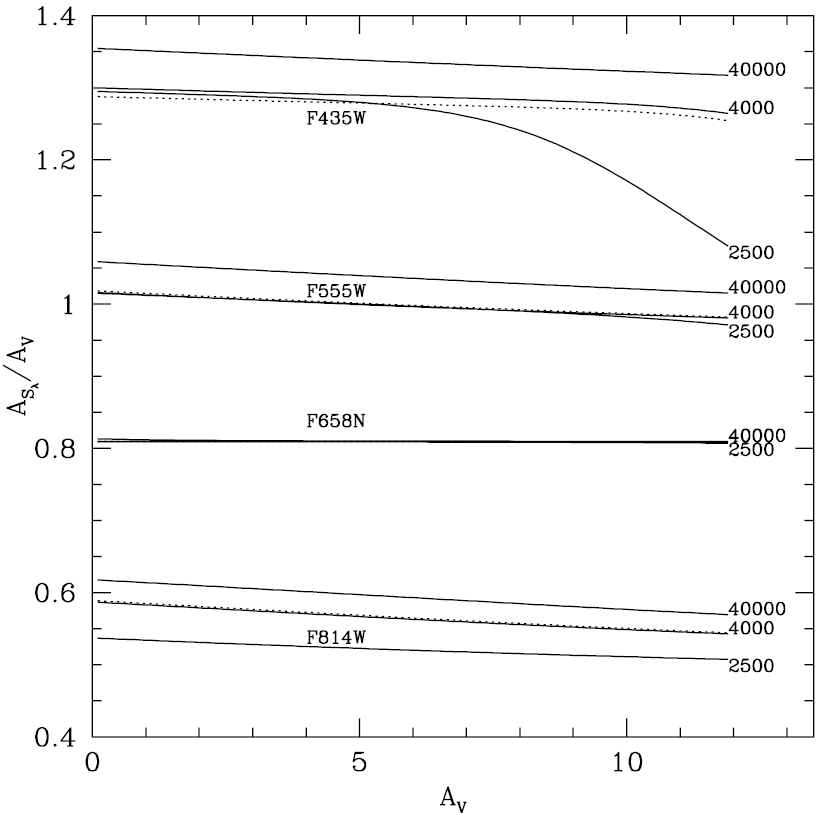
\includegraphics[width=1.0\textwidth]{girardi_forbes_effect_figure.png}
\caption{Plots of $A_{X}/A_{V}$ for selected ACS filters as functions of the initial $A_{V}$ value selected for the calculation of bolometric corrections. Solid lines represent the atmospheres of dwarf stars (log($g$) = 5.0), while dashed lines represent those of giants, which are defined by the relation $T_{\textnormal{eff}} = 3250 + 500\log(g)$. The number next to each line represents the effective temperature of  the atmospheric model being used. The variation of $A_{X}/A_{V}$ with chosen $A_{V}$ simulates the  strength of the Forbes effect. Source: \cite{2008PASP..120..583G}.}
\label{girardi_forbes}
\end{center}
\end{figure}

This has the effect of producing a non-linear increase in extinction for one filter relative to the increase in another \citep{1995A&AS..109..293G,2008PASP..120..583G}. It should be emphasised that the Forbes effect occurs regardless of the source star's spectral type, and therefore represents an additional source of uncertainty when calculating extinction for highly-reddened stellar populations. \\*

The Forbes effect has an impact on the non-zero $A_{V}$ value chosen for Equation \ref{BCs_diff} because if $R_{V}$ is held constant at the standard diffuse ISM value of 3.1 \citep{1989ApJ...345..245C}, a larger $A_{V}$ value implies a longer path through the ISM, and thus a stronger Forbes effect. According to \cite{2008PASP..120..583G}, any significant impact from the Forbes effect on the values of $A_{X}/A_{V}$ occurs for a chosen $A_{V} \gtrsim 4$. This is illustrated in Figure \ref{girardi_forbes}, where the difference between the $A_{X}/A_{V}$ values at the lowest chosen $A_{V}$ values and higher values only becomes significant at $A_{V}$ values above 4.

They found that the effect was particularly strong for stars with $T_{\textnormal{eff}} \lesssim 3000$K, as shown in the bluer filters in Figure \ref{girardi_forbes},  and that, unsurprisingly, it became greater as the wavelength range covered by the filter response function increased. This is shown in Figure \ref{girardi_forbes} by the absence of any significant Forbes effect in the very narrow F658N WFPC2 filter, whose effective width is only 28.5 \AA \citep{2008wfpi.book.....M}.\\*

\subsubsection{Comparison with observed clusters}

An $A_{V}$ value of 1.0 represents a cluster environment with an overall extinction which is high, but still realistic, when compared to extinction in observed star clusters. This assessment is justified according to the data in Table 2 of \cite{2019AJ....158...35S}. The $A_{V}$ in that table were obtained by multiplying the listed $E_{B-V}$ values by an $R_{V}$ value of 3.1, as was assumed for the synthetic data in this project. This assumption was justified on the basis that, with only a small number of exceptions, these clusters were assessed by \cite{2019AJ....158...35S} as obeying the Milky Way law for extinction as a function of wavelength, which is the same as that employed in the seminal extinction-modelling studies, such as \cite{1989ApJ...345..245C}. As shown in Figure \ref{siegel_Av_vals}, out of the 49 open clusters in the table, only 3 have $A_{V}$ values greater than 1.0. However, the largest $A_{V}$ value calculated was 2.17. This result puts the $A_{V}$ value of 1.0 assumed for this project near the midpoint of the total $A_{V}$ range covered by the clusters in the \cite{2019AJ....158...35S} sample. Therefore, the $A_{V}$ value of 1.0 was assessed as realistic in the context of observed star clusters.

\begin{figure}[h!]
\begin{center}
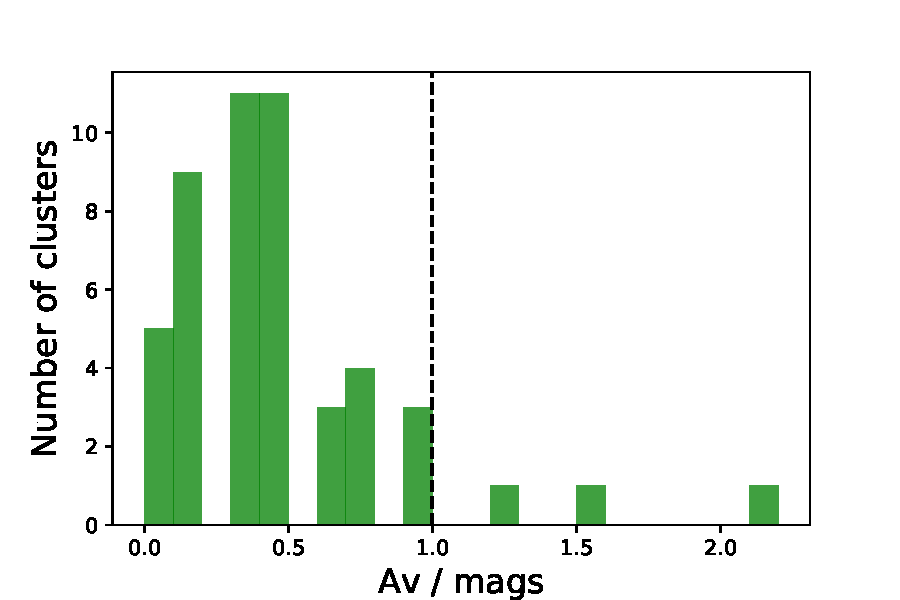
\includegraphics[width=1.0\textwidth]{../siegel_clusters_Av_vals_hist.pdf}
\caption{Histogram of $A_{V}$ values of clusters listed in Table 2 of \cite{2019AJ....158...35S}. The $A_{V}$ bins have a uniform width of 0.1 magnitudes. The vertical dashed line at $A_{V}$ = 1.0 represents the value selected in this project.}
\label{siegel_Av_vals}
\end{center}
\end{figure}

\section{Filters studied} \label{filter_desc}
In this project, three broad-band filter systems were employed. Two are systems on board the Hubble Space Telescope (HST). These are the Advanced Camera for Surveys (ACS), installed in 2002 on the HST \citep{2007AJ....133.1658S}, and the Ultraviolet Imaging Spectrograph channel of the Wide-Field Camera 3 (WFC3/UVIS), installed on the HST in 2009 \citep{2010wfc..rept...14K,2010SPIE.7731E..0ZM}. The third is the single set of three broadband filters mounted on the Gaia space observatory \citep{2010A&A...523A..48J,2018A&A...616A...4E}, launched in 2013. \\*

\begin{table}
\begin{center}
\begin{tabular}{cccccc}
\hline
System & Filter & $\lambda_{\textnormal{cen}}$ / \AA & FWHM / \AA & $\lambda_{\textnormal{min}}$ / \AA & $\lambda_{\textnormal{max}}$ / \AA \\
\hline
% results: previously listed & from source website specified in caption					added more info: l_min & l_max
& F435W & 4359 & 881 & 3610 & 4860 \\ % & 4760 & 729
& F475W & 4781 & 1403 & 3863 & 5563 \\ % & 5000 & 986
& F555W & 5413 & 1236 & 4584 & 6209 \\ % & 5060 & 841
ACS & F606W & 5961 & 2255 & 4634 & 7180 \\ % & 6690 & 1566
& F625W & 6323 & 1390 & 5446 & 7100 \\ % & 6480 & 978
& F775W & 7763 & 1517 & 6804 & 8632 \\ % & 7320 & 1017
& F814W & 8117 & 2096 & 6885 & 9648 \\ % & 7460 & 1657
\hline
& F218W & 2216 & 329 & 1990 & 2603 \\ % & 2175 & 300
& F225W & 2341 & 464 & 1990 & 2968 \\ % & 2250 & 500
& F275W & 2696 & 417 & 2282 & 3119 \\ % & 2750 & 500
& F300X & 2722 & 660 & 2137 & 4098 \\ % &  & 2775
& F336W & 3368 & 550 & 3014 & 3707 \\ % & 3375 & 550
& F390W & 3929 & 951 & 3255 & 4470 \\ % & 3900 & 1000
WFC3 & F438W & 4322 & 674 & 3895 & 4710 \\ % & 4320 & 695
& F475W & 4768 & 1482 & 3942 & 5582 \\ % & 4750 & 1520
& F555W & 5262 & 1578 & 4381 & 7045 \\ % & 5410 & 1605
& F606W & 5941 & 2298 & 4700 & 7204 \\ % & 5956 & 2340
& F625W & 6274 & 1573 & 5414 & 7138 \\ % & 6250 & 1550
& F775W & 7725 & 1454 & 6869 & 8571 \\ % & 7760 & 1470
& F814W & 7814 & 1505 & 6978 & 9684 \\ % & 8353 & 2555
\hline
& $G$ & 6631 & 4397 & 3321 & 10515 \\ % & 6730 & 4400
Gaia & $G_{\textnormal{bp}}$ & 5330 & 2530 & 3283 & 6714 \\ % & 5320 & 2530
& $G_{\textnormal{rp}}$ & 7896 & 2956 & 6296 & 10637 \\ % & 7970 & 2960
\hline

\end{tabular}
\caption{Basic properties of the filters employed in this project. See text for details. Source: \protect\url{http://svo2.cab.inta-csic.es/svo/theory/fps3/index.php}}
\label{filter_basics}
\end{center}
\end{table}

In Table \ref{filter_basics}, all the filters used for this project are listed. The name of each filter is displayed alongside its central wavelength ($\lambda_{\textnormal{cen}}$), full-width at half-maximum (FWHM) and the minimum ($\lambda_{\textnormal{min}}$) and maximum ($\lambda_{\textnormal{max}}$) detection wavelengths. Hence, when combined, these filters cover wavelengths from the soft-ultraviolet (soft-UV) to the near-infrared (NIR), including all visible wavelengths. The FWHM is defined as the difference between the lowest and highest wavelength values at which the transmittance value is half of its maximum value for the filter, typically assuming the response function can be approximated as a Gaussian distribution centred on the central wavelength. The FWHM acts as an approximate measure of the wavelength range within which the filter can be used for observations.\\*

The response functions for the three filter systems employed in this project are shown in Figures \ref{Gaia_response_funcs}-\ref{WFC3_response_funcs2}. By comparing these with the filters' information in Table \ref{filter_basics}, it can be seen that the exact shape of the response function has a substantial impact on the observed flux, as shown in its contribution to the value of the apparent magnitude in Equation \ref{app_mag_def} and the filter effective wavelength in Equation \ref{eff_wavelength_def}, which in turn necessitates the use of colour corrections, as detailed in Section \ref{colour_corr}.\\*

Reference will also be made to the Johnson-Cousins UBVRI filter system \citep{1953ApJ...117..313J,1990PASP..102.1181B}, particularly the $V$ filter as all extinction quantities used in this project are normalised to the value of extinction in this filter, $A_{V}$. \\*

\begin{figure}[h!]
\begin{center}
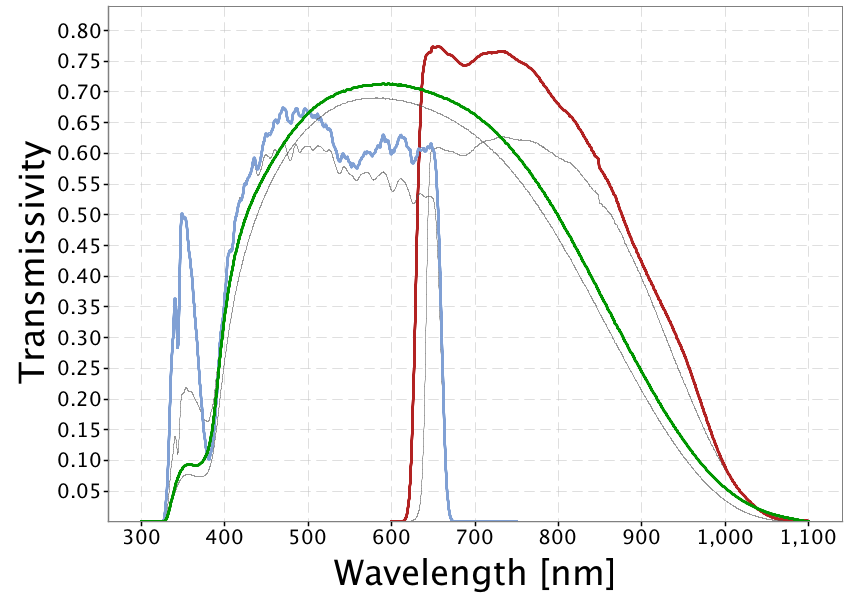
\includegraphics[width=1.0\textwidth]{GaiaDR2Passbands.png}
\caption{Filter response functions for Gaia broadband photometric filters. The three coloured curves show the response functions for the $G$ (green), $G_{\textnormal{bp}}$ (blue) and $G_{\textnormal{rp}}$ (red) filters as used for Gaia Data Release 2 \citep{2018A&A...616A...4E}. These three DR2 curves were employed for all Gaia-related calculations in this project. The three grey curves show the nominal response functions for the same filters as described in the pre-launch stage by \cite{2010A&A...523A..48J}. These grey curves were used for Gaia DR1 only. Source: \protect\url{https://www.cosmos.esa.int/web/gaia/iow_20180316}, adapted from \cite{2018A&A...616A...4E}.}
\label{Gaia_response_funcs}
\end{center}
\end{figure}

\begin{figure}[h!]
\begin{center}
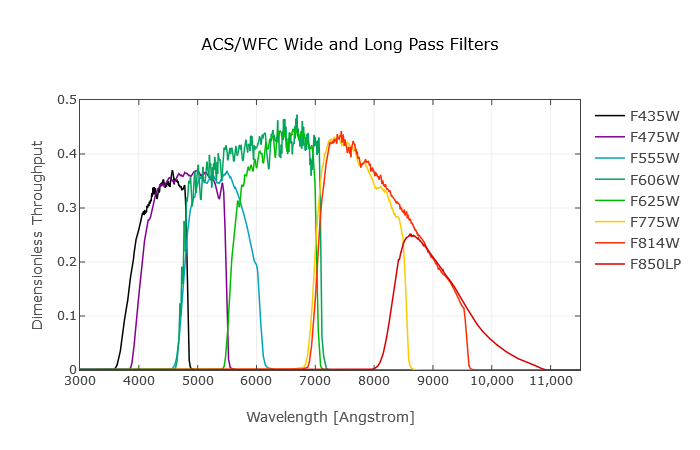
\includegraphics[width=1.0\textwidth]{ACS_Wide.png}
\caption{Filter response functions for wide-field ACS filters. Source: \protect\url{http://www.stsci.edu/hst/acs/analysis/throughputs}}
\label{ACS_response_funcs}
\end{center}
\end{figure}

\begin{figure}[h!]
\begin{center}
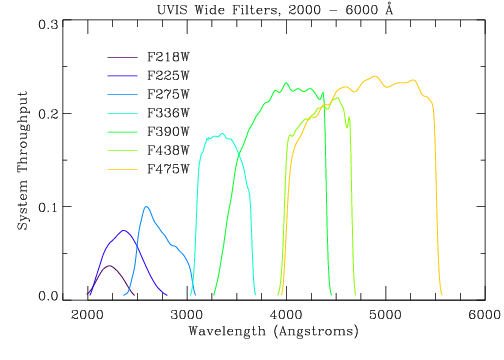
\includegraphics[width=1.0\textwidth]{UVIS_Wide1.jpg}
\caption{Filter response functions for wide-field WFC3 filters. Source: \protect\url{http://www.stsci.edu/hst/wfc3/ins_performance/throughputs/UVIS_filterthru.html}}
\label{WFC3_response_funcs1}
\end{center}
\end{figure}

\begin{figure}[h!]
\begin{center}
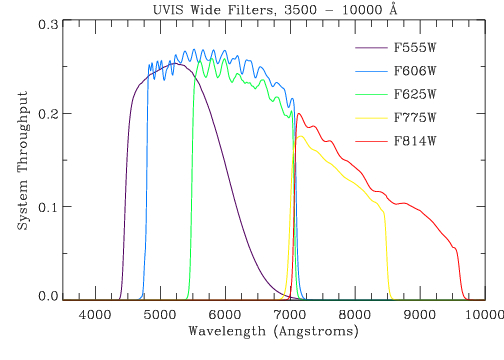
\includegraphics[width=1.0\textwidth]{UVIS_Wide2.jpg}
\caption{Filter response functions for wide-field WFC3 filters. Source: \protect\url{http://www.stsci.edu/hst/wfc3/ins_performance/throughputs/UVIS_filterthru.html}}
\label{WFC3_response_funcs2}
\end{center}
\end{figure}

The standard treatment of extinction for isochrones in CMDs is to apply a single constant value of the extinction ratio for a given filter $X$ to all objects in the isochrone. This quantity is usually expressed as a fixed extinction ratio $A_{X}/A_{V}$ of the (constant) coefficient value in the Johnson-$V$ filter, the standard visual comparison filter. This value is maintained for all stars, regardless of the different effective temperatures, metallicities or surface gravities of the different types of stars present in any given population. The wavelengths of optical light lie between 3800 \AA\ and 7400 \AA, with the $V$ filter having a central wavelength of 5500 \AA.


\section{Variations in extinction ratio data due to stellar atmospheres} \label{desc_var}

The data showing variations in the $A_{X}/A_{V}$ data, generated via Equations \ref{BC_extinc} and \ref{BCs_diff}, with stellar effective temperature are shown for the WFC3 and Gaia filters in Figure \ref{just_data_FeH0_WFC3gaia} and for the ACS filters in Figure \ref{just_data_FeH0_ACS}. \\*

For all filters described in Section \ref{filter_desc}, the greatest variations in the $A_{X}/A_{V}$ data occur with changes in $T_{\textnormal{eff}}$, with changes due to log($g$) and [Fe/H] being much less significant. This is to be expected, given that the value of $T_{\textnormal{eff}}$ has a significant effect on the magnitude and shape of the stellar spectral energy distribution (see Figure \ref{planck_curve}), while the effects of the surface gravity and metallicity are restricted to the absorption lines in the SED, as discussed in Section \ref{params}. Plots of $A_{X}/A_{V}$ against $T_{\textnormal{eff}}$ for atmospheres at solar metallicity are presented in Figure \ref{just_data_FeH0_WFC3gaia} for the WFC3 and Gaia filters and Figure \ref{just_data_FeH0_ACS} for the ACS filters. \\*

\begin{figure}[h!]
\begin{center}
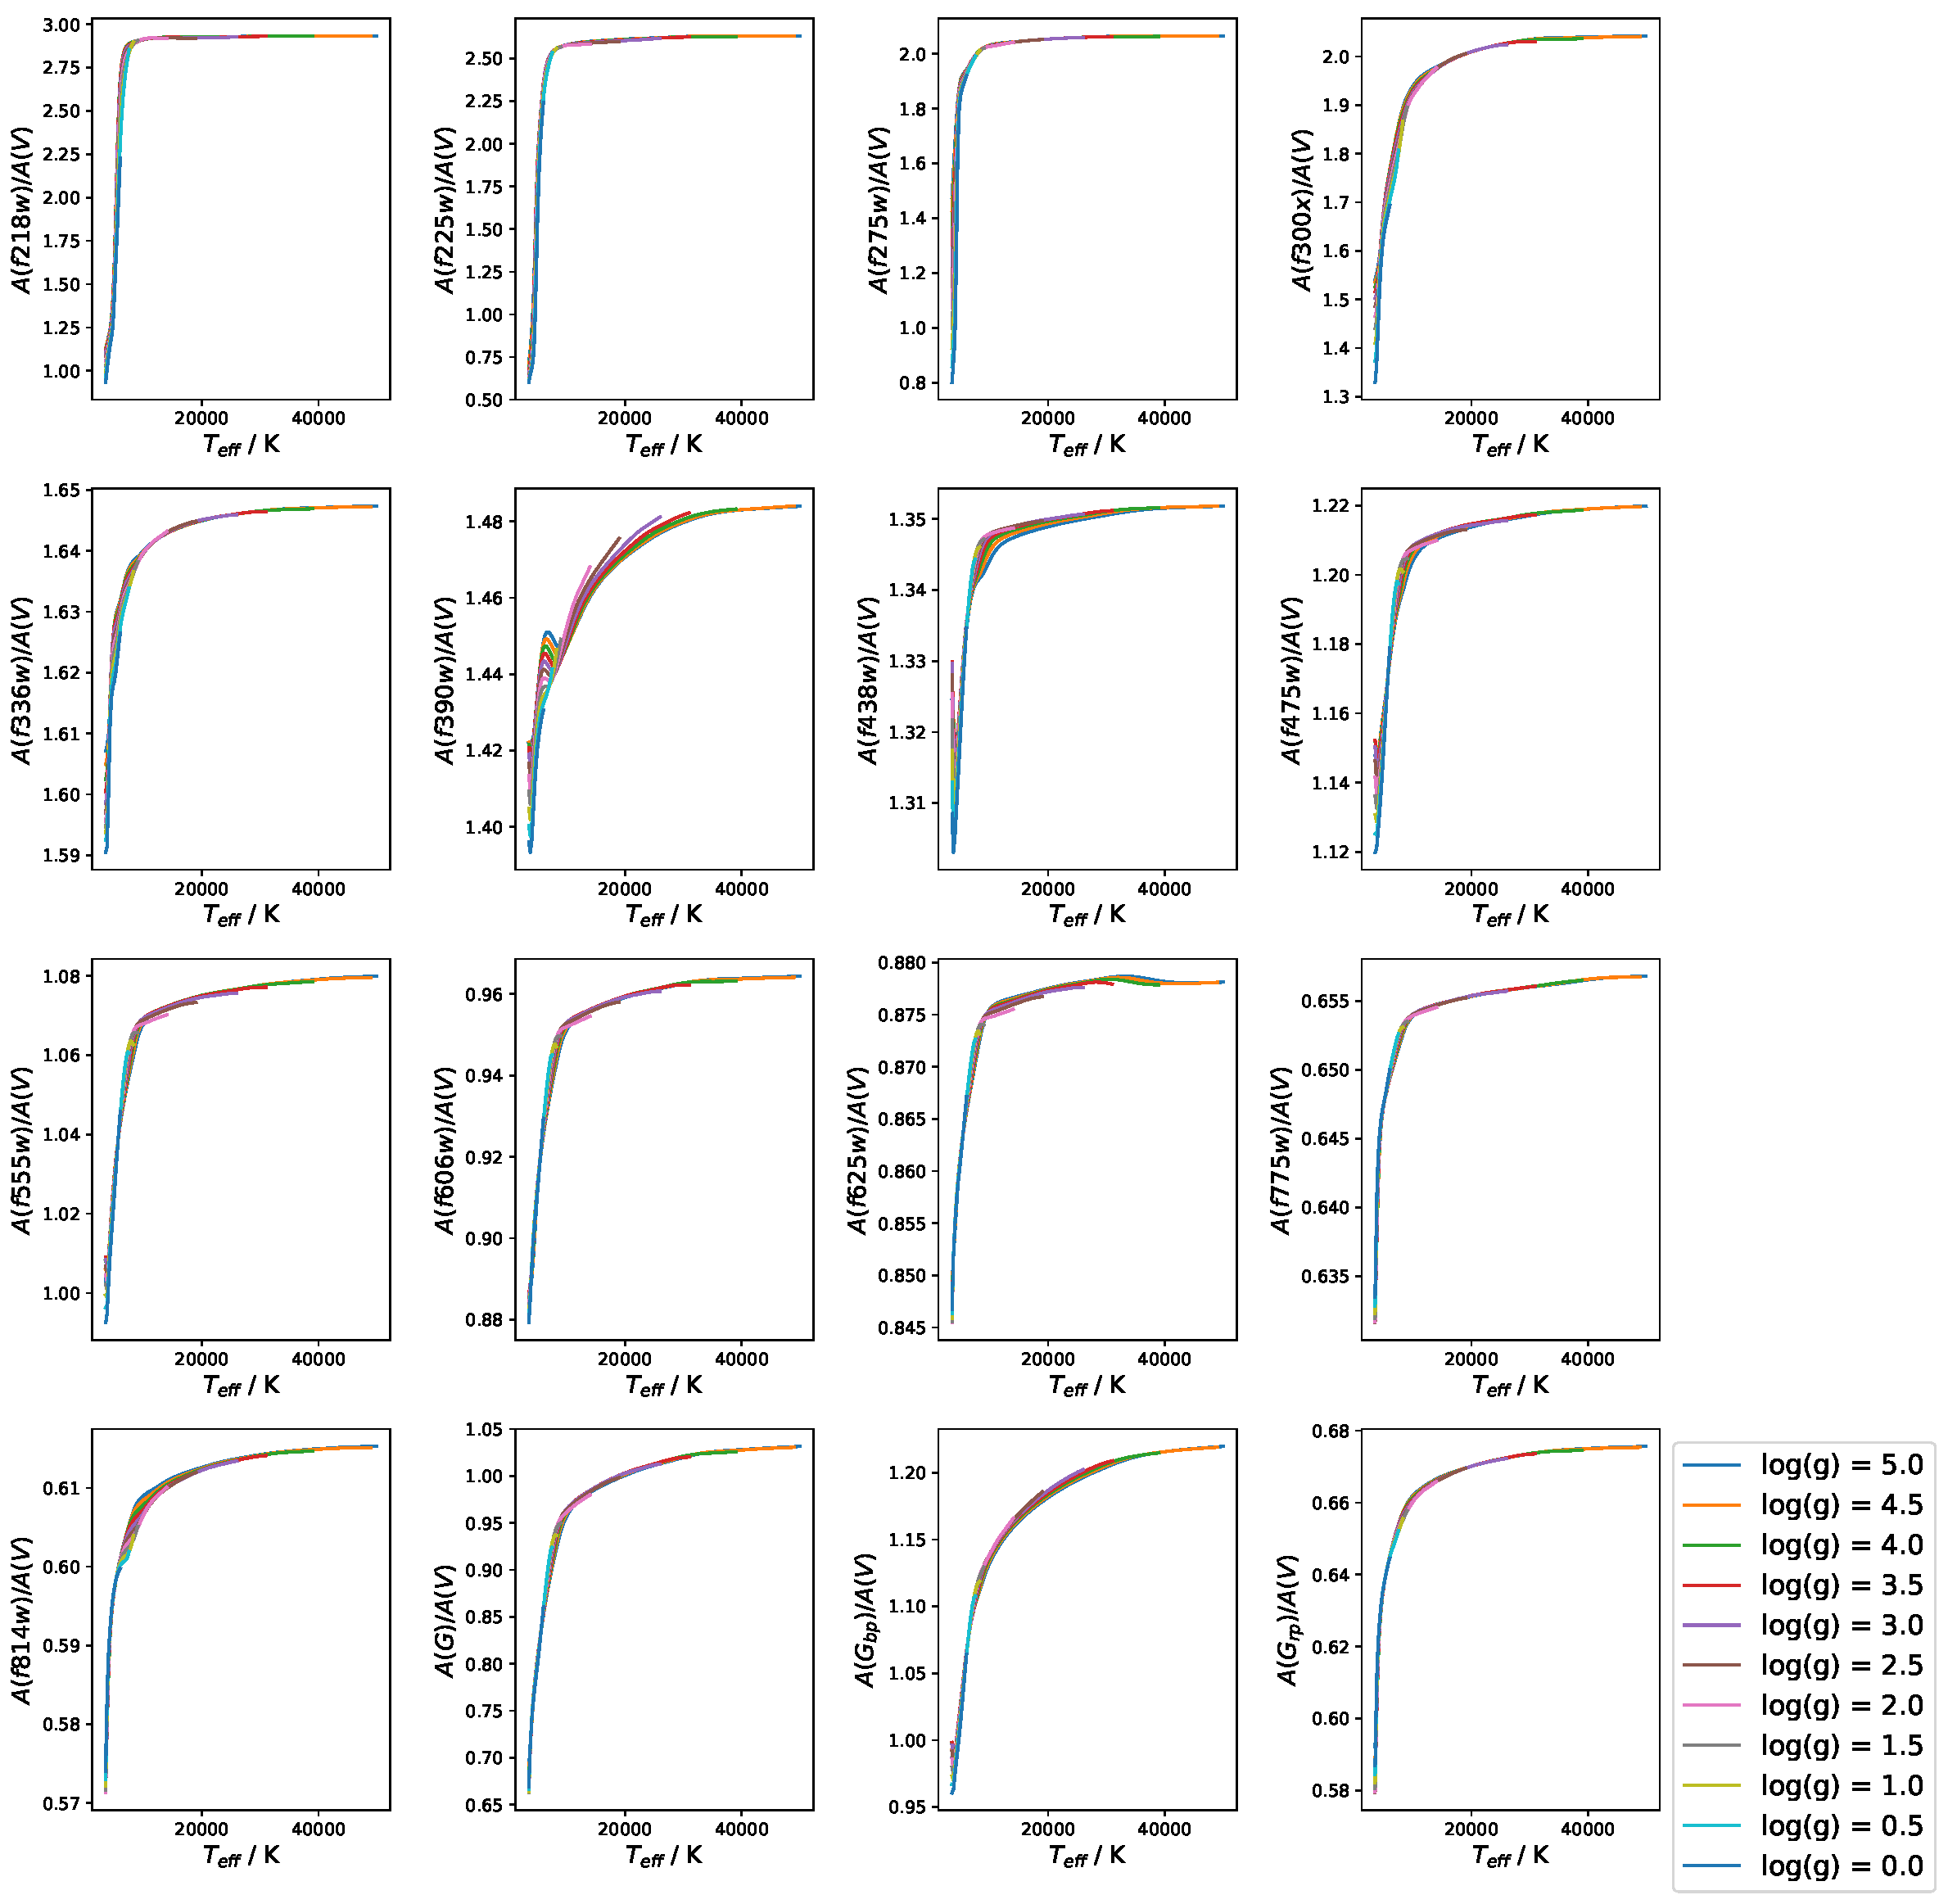
\includegraphics[width=0.85\paperwidth]{../just_full_data/comb/AHub_FeH0p0_just_Teff_plot_lines.pdf}
\caption{Solar-metallicity extinction ratio data for the WFC3 (first 13 panels) and Gaia (last 3) systems, with point-to-point lines connecting datapoints for a fixed log($g$) value.}
\label{just_data_FeH0_WFC3gaia}
\end{center}
\end{figure}

\begin{figure}[h!]
\begin{center}
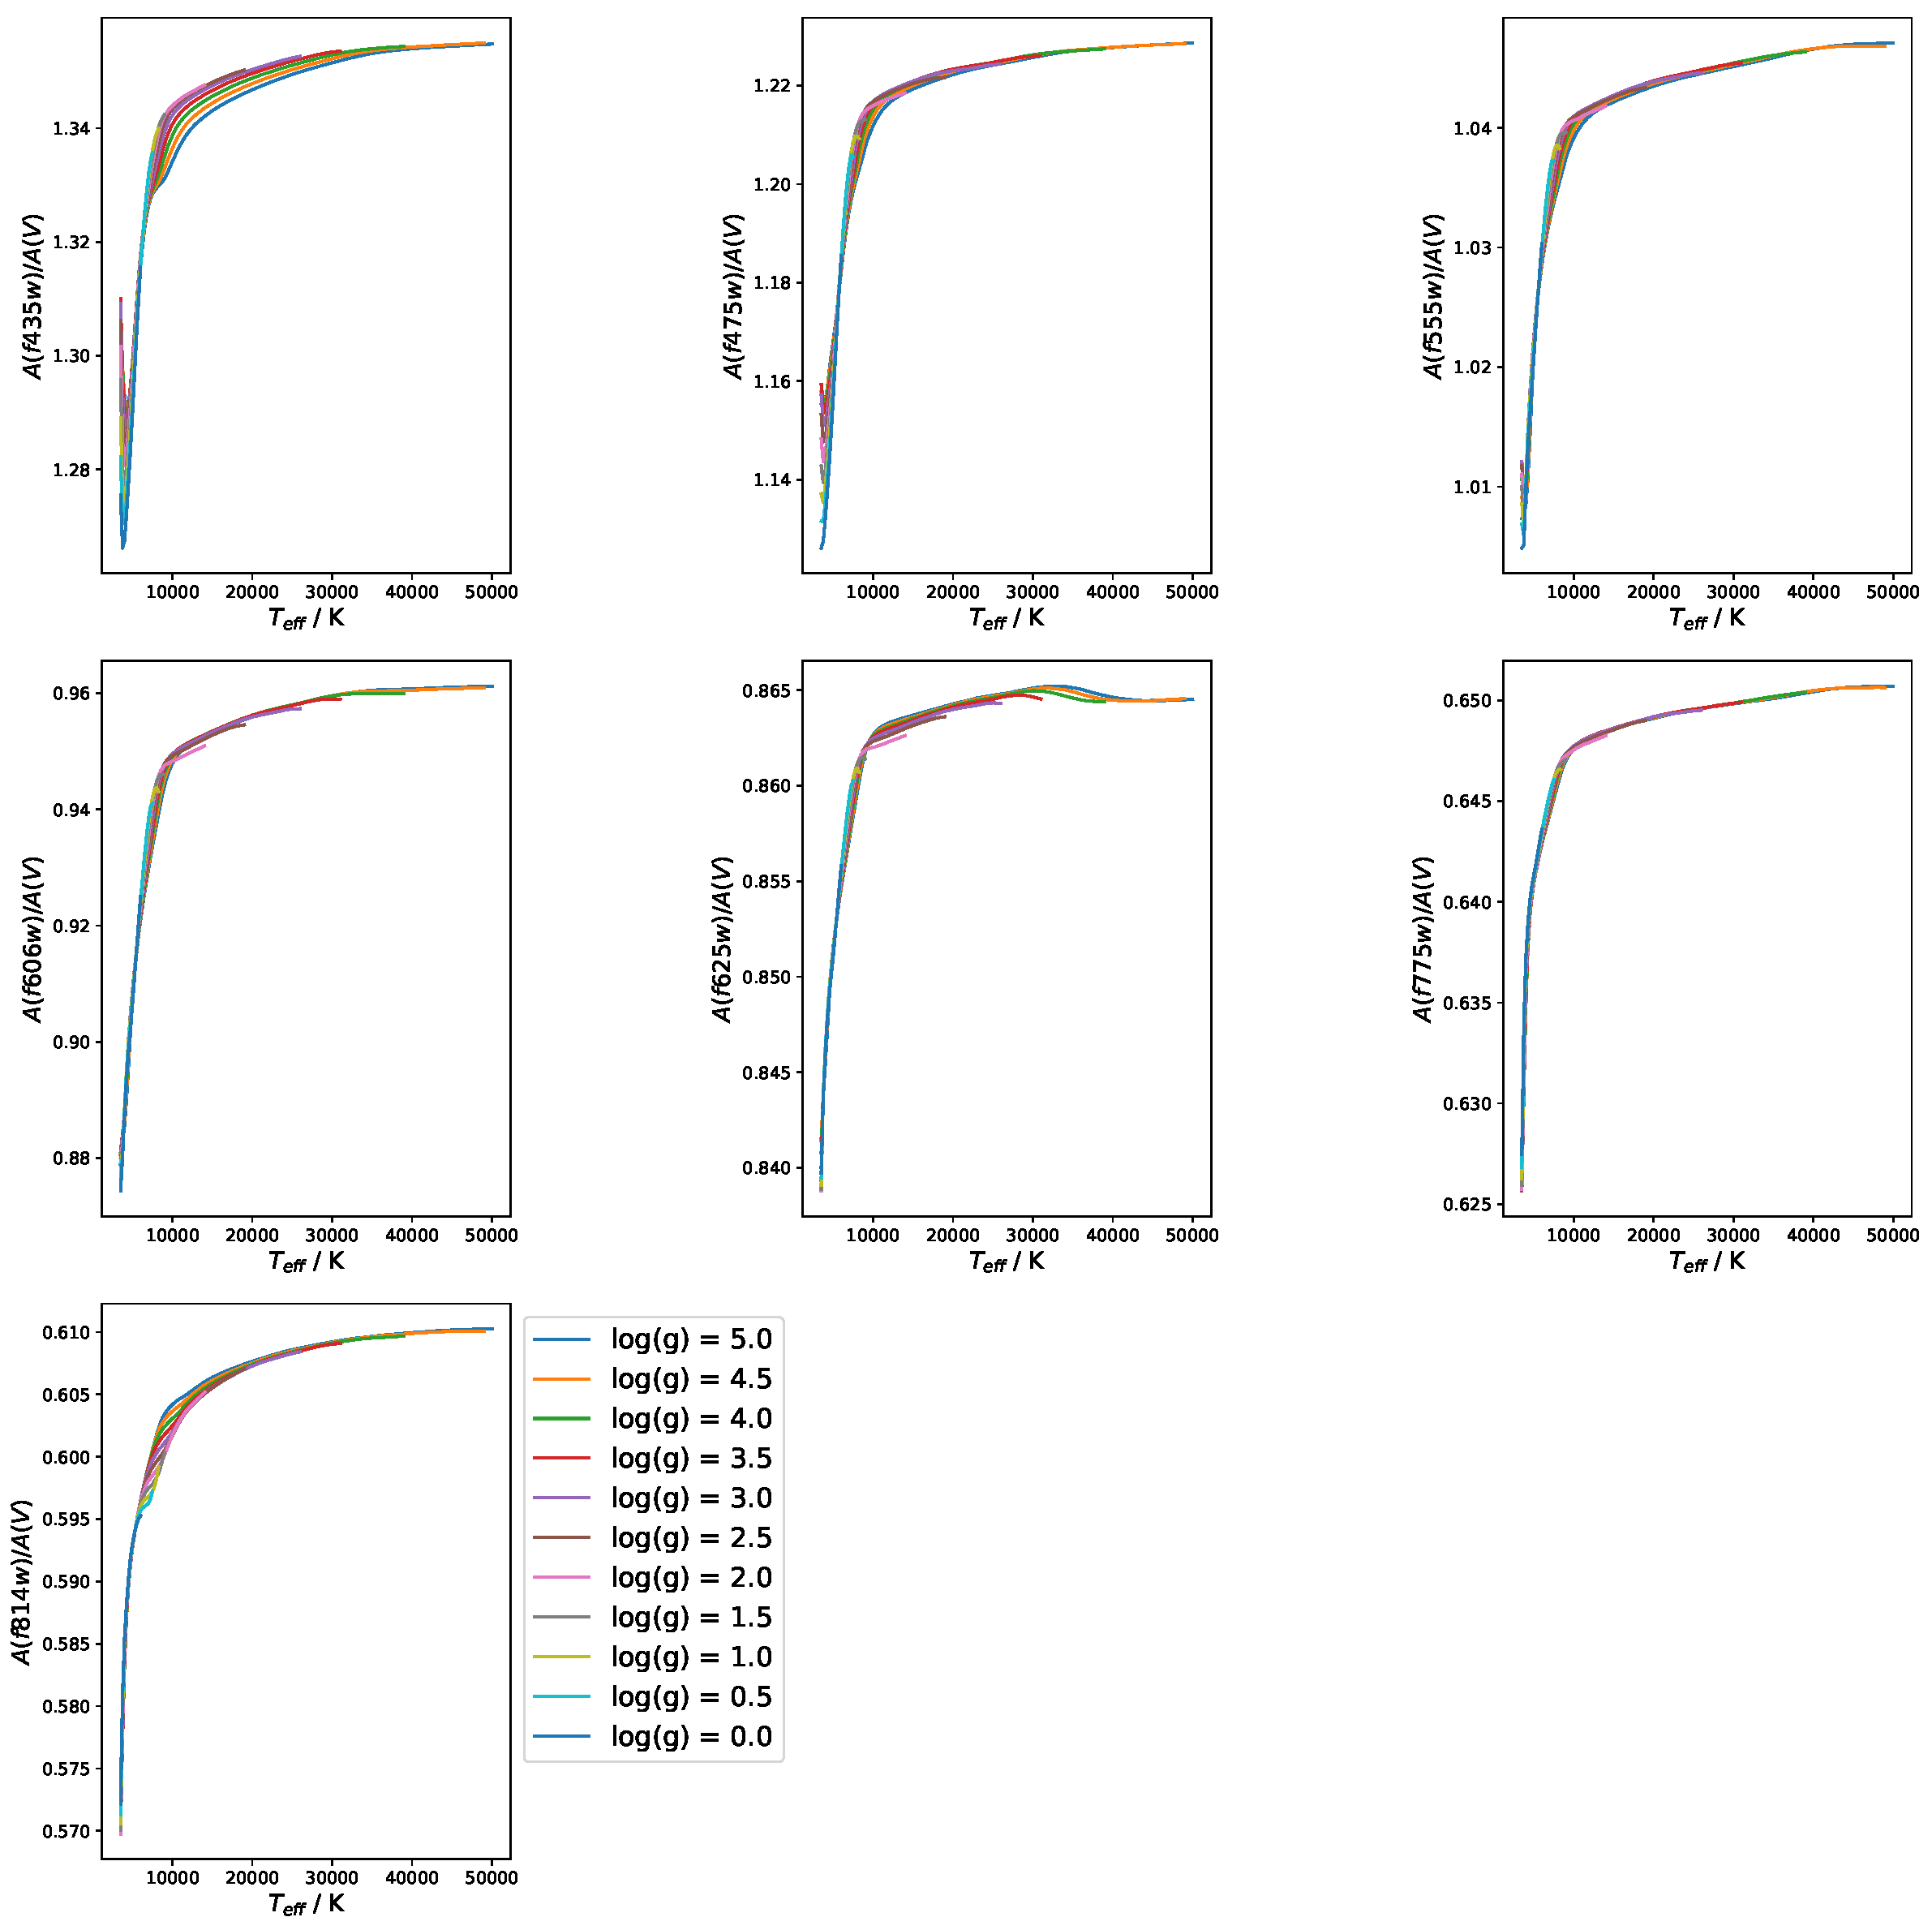
\includegraphics[width=1.0\textwidth]{../just_full_data/ACS/AHub_FeH0p0_just_Teff_plot_lines.pdf}
\caption{Same as Figure \ref{just_data_FeH0_WFC3gaia}, except the filters shown here are for the ACS system.}
\label{just_data_FeH0_ACS}
\end{center}
\end{figure}

Another general feature is the convergence of $A_{X}/A_{V}$ to a single maximum value in each filter, at $T_{\textnormal{eff}} = 50,000$ K, for higher effective temperatures, independent of metallicity and surface gravity. In most filters, this convergence is achieved to within a margin of 0.01 from the value at $T_{\textnormal{eff}} = 50,000$ K at around temperatures of 20,000 K. The region of parameter space in $T_{\textnormal{eff}}$, log($g$) and [Fe/H] characterised as having achieved this convergence will be referred to henceforth as the ``high-$T_{\textnormal{eff}}$ plateau region'' or simply ``plateau''.\\*

In general, the values of $A_{X}/A_{V}$ for a given stellar atmosphere increase as the central wavelength of the filter decreases, reflecting the greater extinction effect of the ISM dust in the UV and optically blue spectral regions, as detailed in Section \ref{ext_def}. This can be seen by looking at the scales on the y-axes of the respective sub-plots in Figures \ref{just_data_FeH0_WFC3gaia} and \ref{just_data_FeH0_ACS}. The UV filters host both the highest plateau $A_{X}/A_{V}$ values and the greatest range in $A_{X}/A_{V}$ between the plateau $T_{\textnormal{eff}}$ region and the lowest-$T_{\textnormal{eff}}$ region. \\*

A property found in the data for some filters, which becomes more pronounced at higher stellar metallicities, is the tendency of the gradient of $A_{X}/A_{V}$ with increasing $T_{\textnormal{eff}}$ to become significantly less positive at the lowest temperatures in the data, typically around 4000K and below. The spread in $A_{X}/A_{V}$ values for different log($g$) is typically about 0.02-0.04, with a linear progression from log($g$) = 5.0 at the lowest end to log($g$) = 0.0 at the highest. In some filters, at the highest metallicities employed ([Fe/H] = 0.0, 0.5), this phenomenon causes the gradient to invert and become significantly negative, reversing the trend found everywhere else in the data, including for the same filters at lower metallicity. Due to the shape of the resulting point-to-point line in these axes, as plotted in both Figures \ref{just_data_FeH0_WFC3gaia} and \ref{just_data_FeH0_ACS}, it has been dubbed the ``tail-flick'' phenomenon. In the same figures, the phenomenon is particularly prominent in the plots for the ACS F435W, WFC3 F438W, F475W (both WFC3 and ACS) and Gaia $G_{\textnormal{bp}}$ filters.\\*

This gradient inversion was treated as an artefact of non-physical origin caused by the known significant uncertainties in ATLAS9 at effective temperatures below 4500K \citep{2004astro.ph..5087C,2008PASP..120..583G}. Furthermore, the spread in $A_{X}/A_{V}$ at low $T_{\textnormal{eff}}$ values due to the tail-flick phenomenon is sufficiently small relative to the $A_{X}/A_{V}$ values at low effective temperatures in every relevant filter to be insignificant in terms of the final effect of extinction on the CMD positions of isochrones. As a result, only data for atmospheres with effective temperatures above those affected by the gradient inversion was used by the algorithm to fit the coefficients of the chosen functions. This was carried out by only using data for atmospheres with $T_{\textnormal{eff}} \geq 4500$K for fitting the initial functions.\\*

It can be seen in the right-hand column of Table \ref{filter_AxAv_ranges} that there are significant variations in the $A_{X}/A_{V}$ data as the parameters describing the model stellar atmosphere are varied. In particular, for the shortest-wavelength WFC3 UV filters, the total range in $A_{X}/A_{V}$ can be greater than 2.0, which, for a chosen $A_{V}$ of 1 mag, means that the extinction for different types of stars can vary by as much as two orders of magnitude. 
This is important as these variations are independent of any effect due to interactions between the emitted light beam and the ISM and arise purely as a result of the type of star being observed. \\*

%Furthermore, the Pearson correlation coefficient for all filters  ****0.760988925385 is the non-UV correlation coefficient\\*

\begin{table}
\begin{center}
\begin{tabular}{ccccc}
\hline
System & Filter & Minimum $A_{X}/A_{V}$ & Maximum $A_{X}/A_{V}$ & Total $A_{X}/A_{V}$ range \\
\hline
% results: previously listed & from source website specified in caption					added more info: l_min & l_max
& F435W & 1.263 & 1.355 & 0.092 \\
& F475W & 1.117 & 1.229 & 0.112 \\
& F555W & 0.998 & 1.047 & 0.049 \\
ACS & F606W & 0.865 & 0.962 & 0.097 \\
& F625W & 0.835 & 0.865 & 0.030 \\
& F775W & 0.624 & 0.651 & 0.027 \\
& F814W & 0.565 & 0.610 & 0.045 \\
\hline
& F218W & 0.897 & 2.935 & 2.038 \\
& F225W & 0.586 & 2.634 & 2.049 \\
& F275W & 0.773 & 2.065 & 1.292 \\
& F300X & 1.323 & 2.043 & 0.720 \\
& F336W & 1.587 & 1.647 & 0.060 \\
& F390W & 1.390 & 1.484 & 0.094 \\
WFC3 & F438W & 1.302 & 1.352 & 0.050 \\
& F475W & 1.110 & 1.220 & 0.110 \\
& F555W & 0.977 & 1.080 & 0.103 \\
& F606W & 0.869 & 0.965 & 0.094 \\
& F625W & 0.841 & 0.879 & 0.038 \\
& F775W & 0.629 & 0.657 & 0.028 \\
& F814W & 0.566 & 0.615 & 0.049 \\
\hline
& $G$ & 0.636 & 1.033 & 0.397 \\
Gaia & $G_{\textnormal{bp}}$ & 0.943 & 1.220 & 0.277 \\
& $G_{\textnormal{rp}}$ & 0.566 & 0.676 & 0.110 \\
\hline

\end{tabular}
\caption{Global minima and maxima (over all combinations of $T_{\textnormal{eff}}$, log($g$) and [Fe/H]) for $A_{X}/A_{V}$ in each of the filters studied in this project.}
\label{filter_AxAv_ranges}
\end{center}
\end{table}

To model the variations in the $A_{X}/A_{V}$ data, functions of $T_{\textnormal{eff}}$, log($g$) and [Fe/H] were created which would be able to describe the variations in $A_{X}/A_{V}$ to a sufficient degree of accuracy. The aim of creating these functions is to reduce the large quantity of data present in the $A_{X}/A_{V}$ tables across all available ATLAS9 atmospheres into a much smaller number of function coefficients while still maintaining a high level of accuracy. For each filter, there was a unique combination of coefficient values and, in certain cases, a new function and number of coefficients.\\*

% with the same information being stored instead as the much smaller number of coefficients for the functions.

To generate the coefficient values and errors, the form of the function was set manually after visually examining the variations in the $A_{X}/A_{V}$ data when plotted against three stellar atmosphere parameters. These functions were then fitted to the data using a least-squares fit algorithm, with the function coefficients acting as the free parameters to be fitted. The acceptable standard deviation in $A_{X}/A_{V}$ for the fit was also set manually. If a particular function form was unable to accurately describe the data, or could not be fitted without producing infeasibly large errors (such as errors the same size as the coefficients) or near-zero errors in one or more coefficients, it was modified or discarded as appropriate. This was repeated until a function could be found for each of the filters studied in this project which could  describe the data to at least a reasonable degree of accuracy, using coefficients with plausible errors. The detailed results of this process are presented in Section \ref{ext_models}.\\*

\section{Isochrone CMD fitting} \label{isoc_fit} 

The functions, whose final forms and coefficients are detailed in Section \ref{ext_models}, were then applied to the isochrone object dataset, producing values of $M_{\textnormal{ext},X}$ for each filter for all objects, in order to match the quantities of distance-corrected observational datasets, with unknown extinction, to those of isochrones. This is that standard procedure used when analysing observational data, as detailed in Section \ref{add_ext}. Thus, the $M_{\textnormal{ext},X}$ (see Equation \ref{MextX_eq}) values for the isochrones and the observational data are being compared.\\*

When comparing the two methods for calculating extinction, in order to test for any differences in the best-fitting isochrone age via the MSTO, a range of ages must be considered. A ``primary'' age was utilised as the true cluster isochrone age. This primary isochrone was subjected to both the function-based (FBER) and fixed extinction-ratio methods. Two isochrones with ages equidistant from the primary were subjected to the standard fixed-extinction method only. All four of the resulting $M_{\textnormal{ext},X}$ isochrones were plotted together in the four chosen CMD axes, together with the original (zero-extinction) isochrone for visual reference.\\*

This procedure was employed for two values of $A_{X}/A_{V}$ for the fixed-extinction treatment. Both were extracted from the ATLAS9 data tables for a log($g$) value of 5.0 to represent a main-sequence star, which is suitable when MSTO positions are being compared. Given the large number of filters studied in this project, four commonly-used CMD axes from among these filters were selected to test for any effects of a $A_{X}/A_{V}$ function. Two of these are specific to the WFC3 system, with one CMD each for ACS and Gaia.\\*

\section{Observational test case: NGC 6793} \label{obs_ngc_section}
To test the effects of the two different treatments of $A_{X}/A_{V}$ on observational data, both were employed to predict the isochrone parameters (age, [Fe/H] and $A_{V}$) for the open cluster NGC 6793. This cluster has little information available in the literature when compared to other open clusters \citep{2019A&A...623A.108B}. Three observational studies have been published which give estimates for the properties of the cluster. The basic cluster properties determined by all three studies are listed in Table \ref{NGC6793_obs}. \\*

NGC 6793 was selected as the test case because it has the significant advantage of having both a high $A_{V}$ extinction value among known star clusters (see the discussion in Section \ref{forbes}) and a full set of Gaia parallax measurements for its member stars. The accurate distances to all its members allows for a higher degree of confidence in the position of the observed cluster CMD. Meanwhile, a high cluster $A_{V}$ value increases any disagreement between the extinction treatments being compared for the cluster. Consequently, any resulting disagreement in estimates of the best-fit isochrone parameters for the cluster become greater and more significant. Furthermore, the presence of multiple studies, all of which disagree on the values of the cluster age and distance and none of which provide a final estimate of the cluster metallicity. Therefore, these studies disagree on the precise location of the isochrone in the CMD, which provides an opportunity to test the effect of changing the method of extinction treatment for multiple published isochrone CMD paths, while keeping the same observational dataset. This makes this cluster more useful as a test case for the effects of changing the extinction-calculation method, which is the ultimate goal of this project.  \\*

\begin{table}
\begin{center}
\resizebox{\textwidth}{!}{\begin{tabular}{cccc}
\hline
Cluster property & K05 & K13 & GC18 \\
\hline
Distance modulus / mag & 10.73 & 9.399 & 8.894 \\
-> distance / pc & 1400 & 724 & 601 \\
log(age / yr) & 8.64 & 8.695 & 8.78 \\
-> Age / Myr & 437 & 495 & 603 \\
$E_{B-V}$ / mag & 0.17 & 0.312 & 0.272 \\
-> $A_{V}$ / mag (if $R_{V} = 3.1$) & 0.53 & 0.967 & 0.843 \\
$\textnormal{[Fe/H]}$ & ? & ? & ? \\
Members & ? (> 3 ACSS-2.5) & 133* & 465 (271 with Gaia photometry)** \\
Parallax / mas & ? & ? & 1.6672 $\pm$ 0.0021 \\
Proper motion (RA) / (mas/yr) & ? & ? & 3.8120 $\pm$ 0.0131 \\
Proper motion (Dec) / (mas/yr) & ? & ? & 3.5622 $\pm$ 0.0136 \\
\hline
\multicolumn{4}{c}{*number of 1$\sigma$ objects inside MWSC "cluster corona border"} \\
\multicolumn{4}{c}{**apparent disagreement between member numbers for clusters listed in Tables 2 and A.4 in GC18.} \\
\end{tabular}}
\caption{Observational parameters for NGC 6793, according to \cite{2005A&A...438.1163K} (K05, WEBDA archive page), \cite{2013A&A...558A..53K} (K13, VizieR archive page) and \cite{2018A&A...616A..10G} (GC18), respectively.}
\label{NGC6793_obs}
\end{center}
\end{table}

\begin{figure}[h!]
\begin{center}
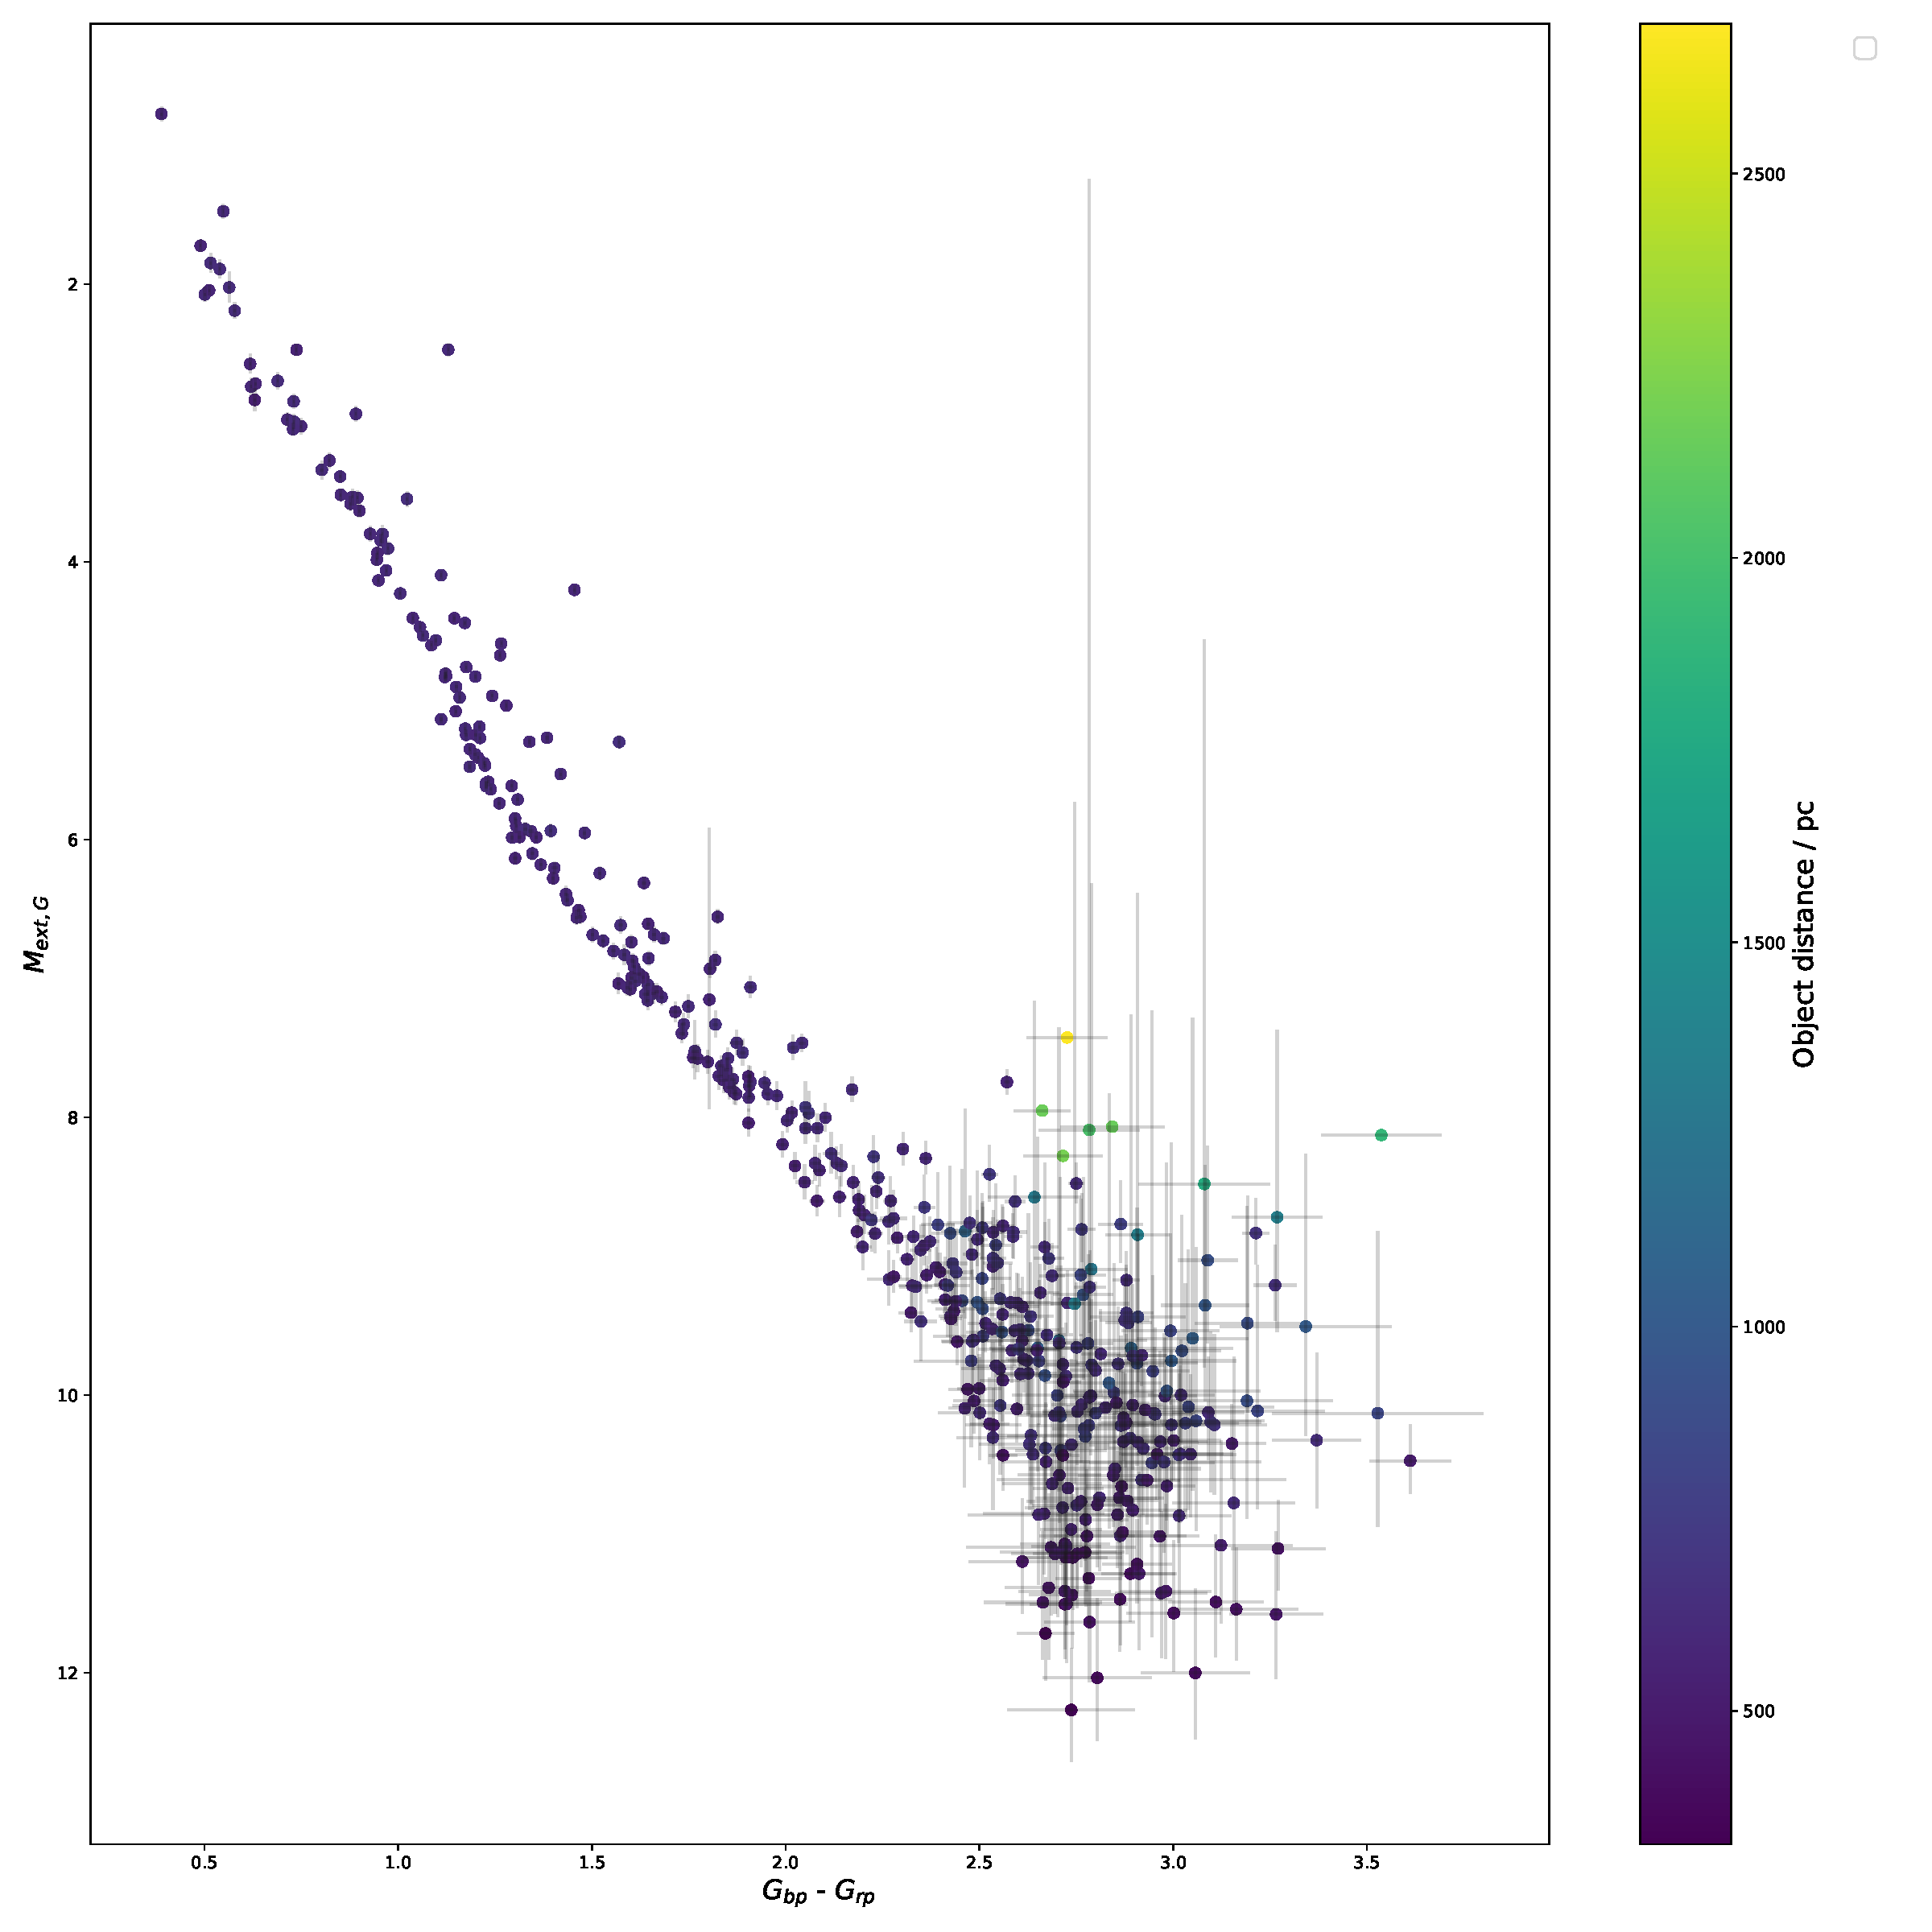
\includegraphics[width=1.0\textwidth]{../NGC_6793_CMD_observational_errorbars_vizier_465.pdf}
\caption{Gaia $G$-($G_{\textnormal{bp}}$-$G_{\textnormal{rp}}$) CMD of NGC 6793, showing the 465 cluster members in the GC18 VizieR table, corrected for their individual distances with errorbars shown. The colour of each object is determined by its parallax-derived distance, while the errorbars are calculated using both photometric and parallax errors.}
\label{NGC_6793_obs_only_465}
\end{center}
\end{figure}

The Gaia DR2 dataset for NGC 6793 was obtained from the VizieR online data catalogue provided by \cite{2018A&A...616A..10G}. The data contained the parallaxes and proper motions (PMs) for both the cluster and its 465 members and the members' apparent magnitudes in all three Gaia filters. All parameters came with error estimates.\\*

The resulting CMD is shown in Figure \ref{NGC_6793_obs_only_465}. The figure shows the full dataset, including objects with distances which appear to lie far outside the expected range based on studies of other open clusters \citep{2006A&A...456..523S}. Therefore, to restrict the dataset to a more realistic stellar population, distance cuts were implemented. The highest cluster radius limit given by \cite{2006A&A...456..523S} was selected initially. Since this value is given as the value for loosely-bound stellar associations, this represents a very low selection threshold.\\*

Since the Gaia data also included PMs for all objects, this information can also be used to test the feasibility of the initial sample of stars. Regarding the PM of cluster members, the membership calculation method of \cite{2003ARep...47..263K} was employed. For each object, this method gives membership probabilities of (a) 61\%,(b) 14\% and (c)$<$1\% if the following conditions are satisfied \citep{2006A&A...446..949D}:

\begin{itemize}
\item the object is within (a) 1$\sigma$, (b) 2$\sigma$ and (c) 3$\sigma$, respectively, of the mean cluster PM (given in Table \ref{NGC6793_obs}).
\item the object is within a photometric error of 1$\sigma$ of the colour index to the left (bluer side) of the zero-age main sequence (ZAMS) in the CMD.
\end{itemize}

The first PM was tested first for the NGC 6793 data. Limits were placed on the deviation of the PM of the member stars from the cluster in both the right ascension and declination directions. The errors on the PMs for the individual stars are between one and three orders of magnitude greater than the error on the cluster PM in both directions. Therefore the $\sigma$ selected for use in both directions was solely that of each respective star. As with the cluster radius criterion, a low membership success threshold of 3$\sigma$ was set for the stellar PM errors. The results of the PM and radius criteria were plotted together to be compared visually in the cluster CMD.\\*

The results are shown in Figure \ref{NGC_6793_cut_effects}. Despite the low threshold of success for both criteria, only 129 stars out of 465 ($\sim$28\%) fulfil both simultaneously. Looking at the results of Figure \ref{NGC_6793_cut_effects} and the distance and errors for the same objects shown in Figure \ref{NGC_6793_obs_only_465}, several conclusions can be drawn:

\begin{itemize}
\item The proper motion criterion is satisfied by a significantly higher number of stars than the radius criterion (340 and 231, respectively).
\item The radius criterion selects almost all of the brightest MS stars in the data, but a significant portion of these (plotted in green) are not selected using the PM criterion.
\item The stars with the most anomalous calculated distances and the highest parallax errors in Figure \ref{NGC_6793_obs_only_465} are nearly all selected using the PM criterion only. These objects are also in the faintest region of the CMD, which likely contributes to their high parallax errors. These objects, in general, were also found to have higher-than-average PM errors among the 465 original members, which is likely to be the cause of their selection by the PM criterion.
\end{itemize}

Even without the additional colour-index constraint from \cite{2003ARep...47..263K} and using a very low membership success threshold, the proper motion criterion results in a CMD with too few bright MS stars. Therefore, using the PM criterion meant that the comparison of isochrone ages using the MSTO region could not be carried out. Consequently, the PM criterion was deemed unnecessary to generate the dataset required for comparing isochrones treated with different extinction calculation methods. \\*

\begin{figure}[h!]
\begin{center}
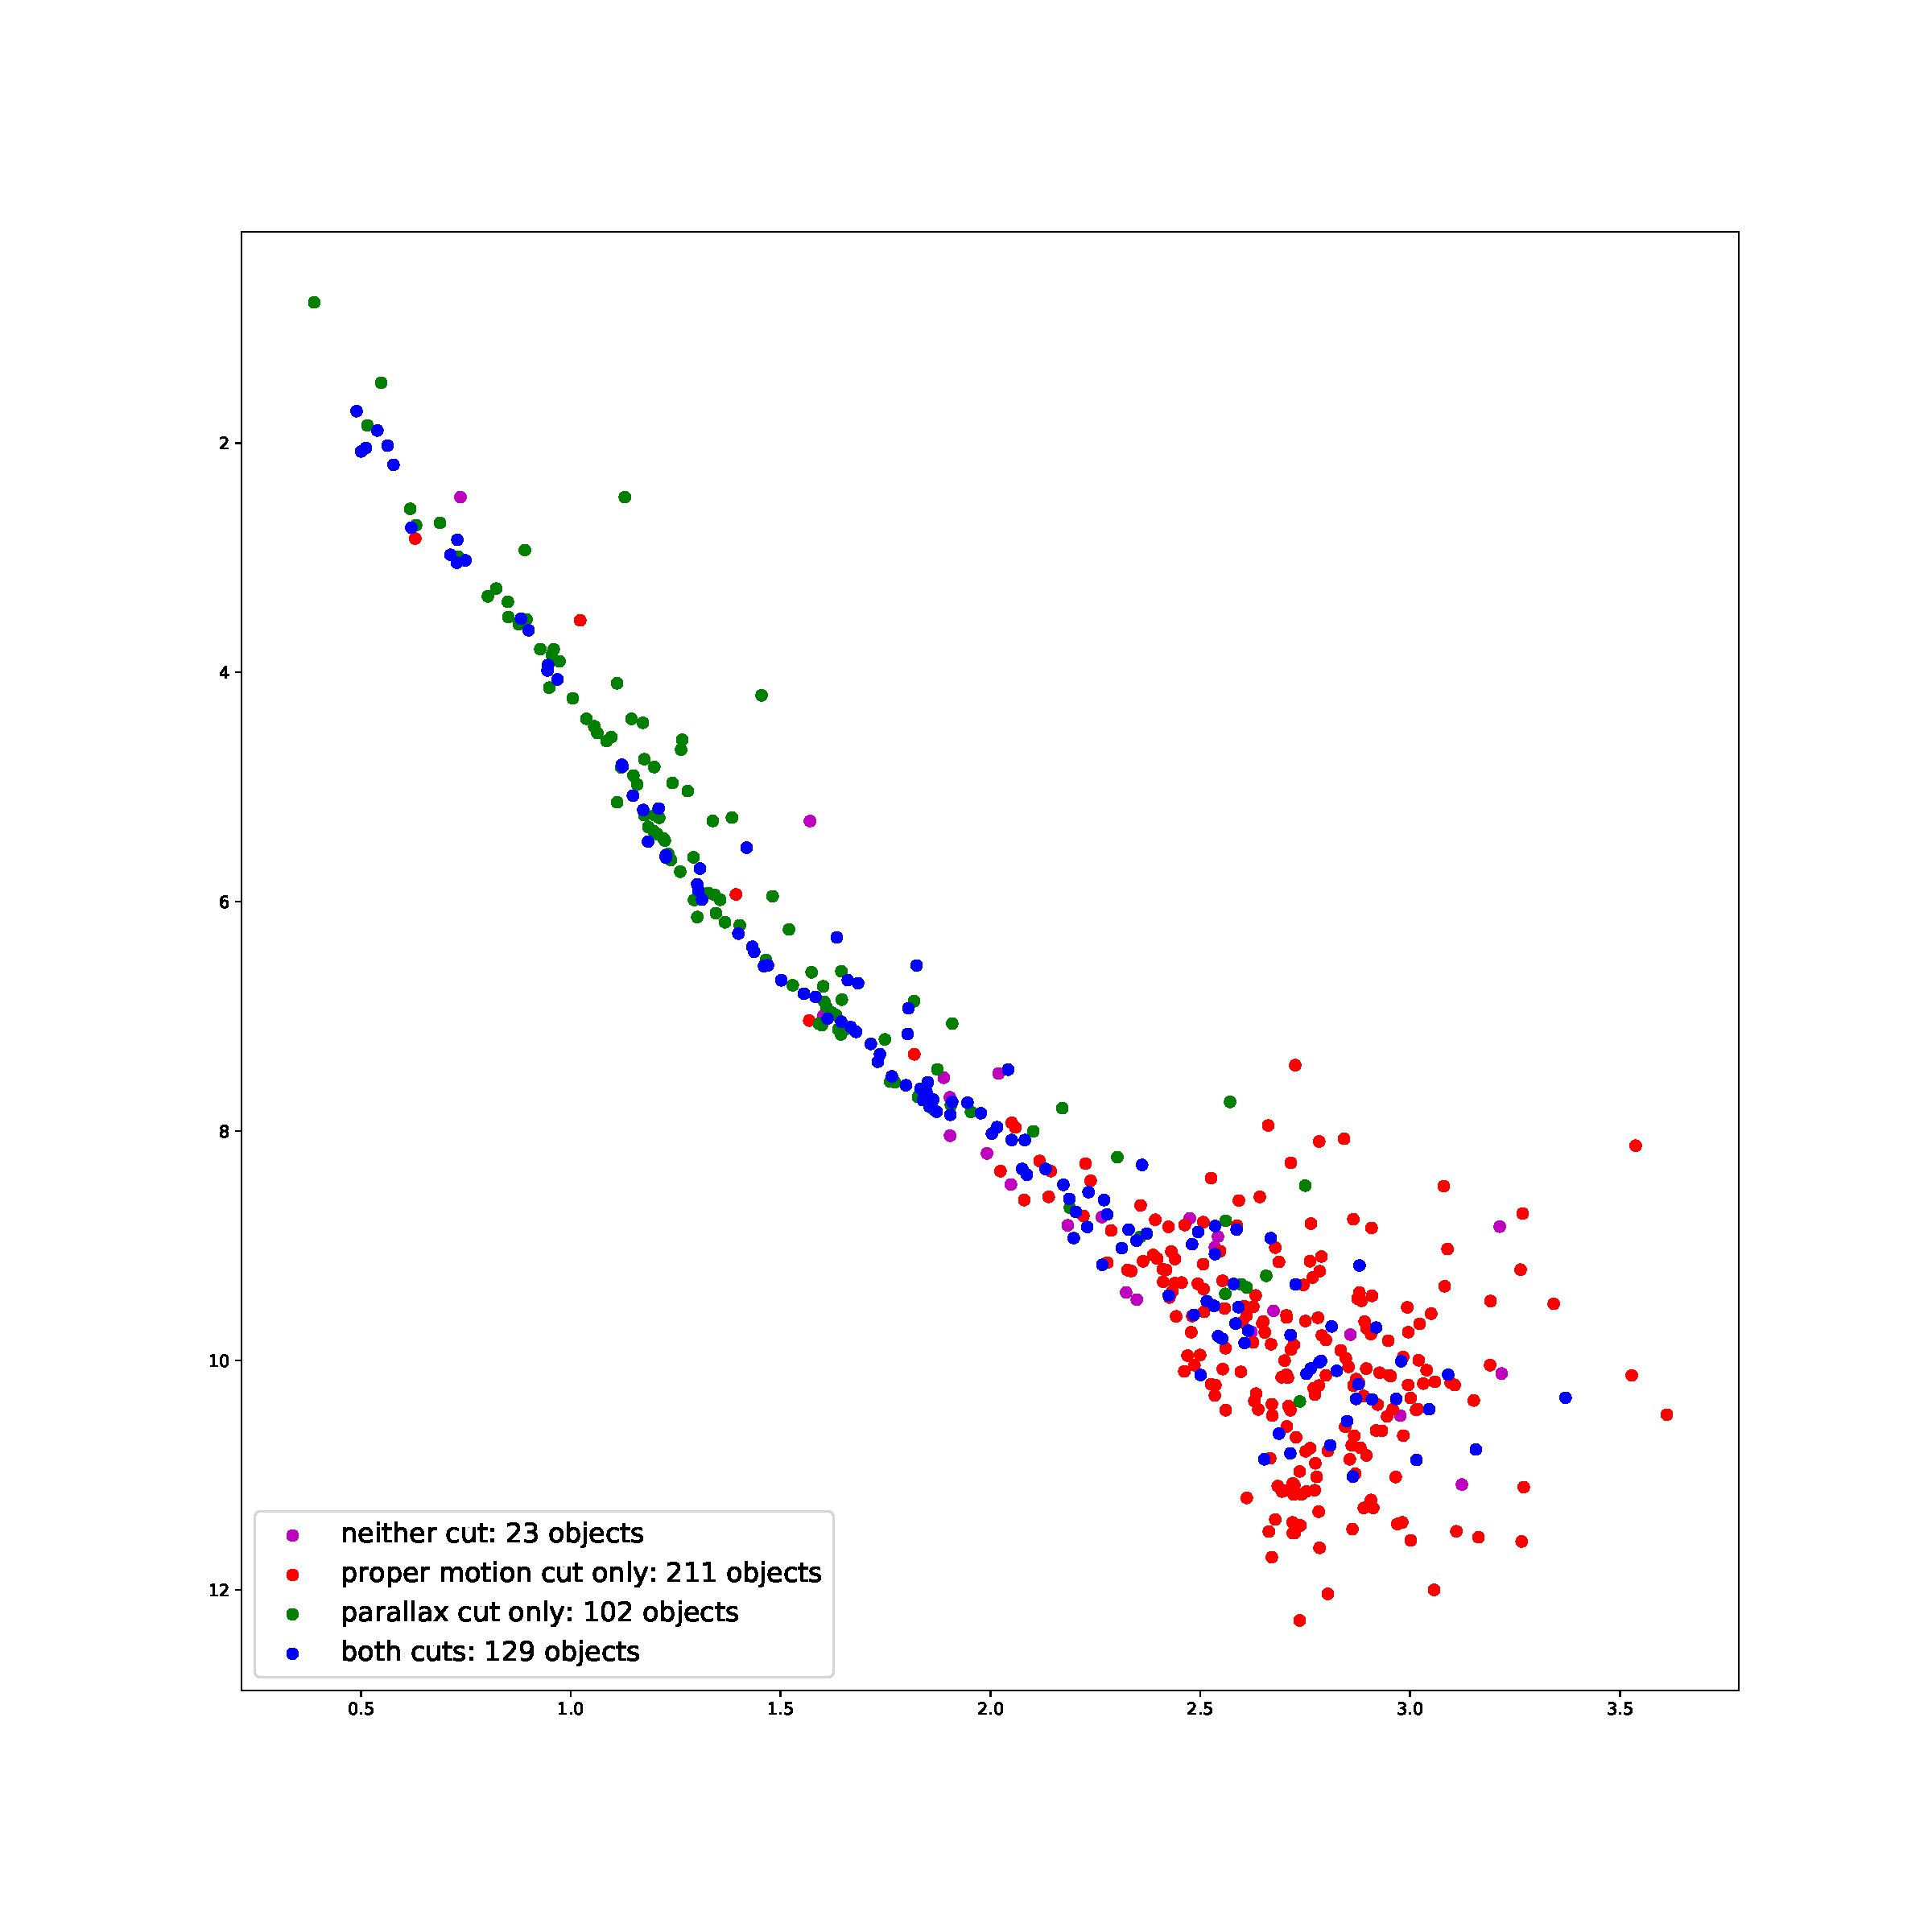
\includegraphics[width=1.0\textwidth]{../NGC6793_pm3sig_vs_plx_cuts_obs_cmd_schilbach.pdf}
\caption{CMD showing all 465 NGC 6793 cluster source objects from the initial dataset. The colour indicates the membership likelihood of each source. The stars with the highest likelihood (in blue) are those which satisfy both the proper motion and cluster radius criteria. Those which fulfil only the proper motion criterion are shown in red and those which fulfil only the radius criterion are in green. Purple points indicate stars which fulfil neither criterion.}
\label{NGC_6793_cut_effects}
\end{center}
\end{figure}

\begin{figure}[h!]
\begin{center}
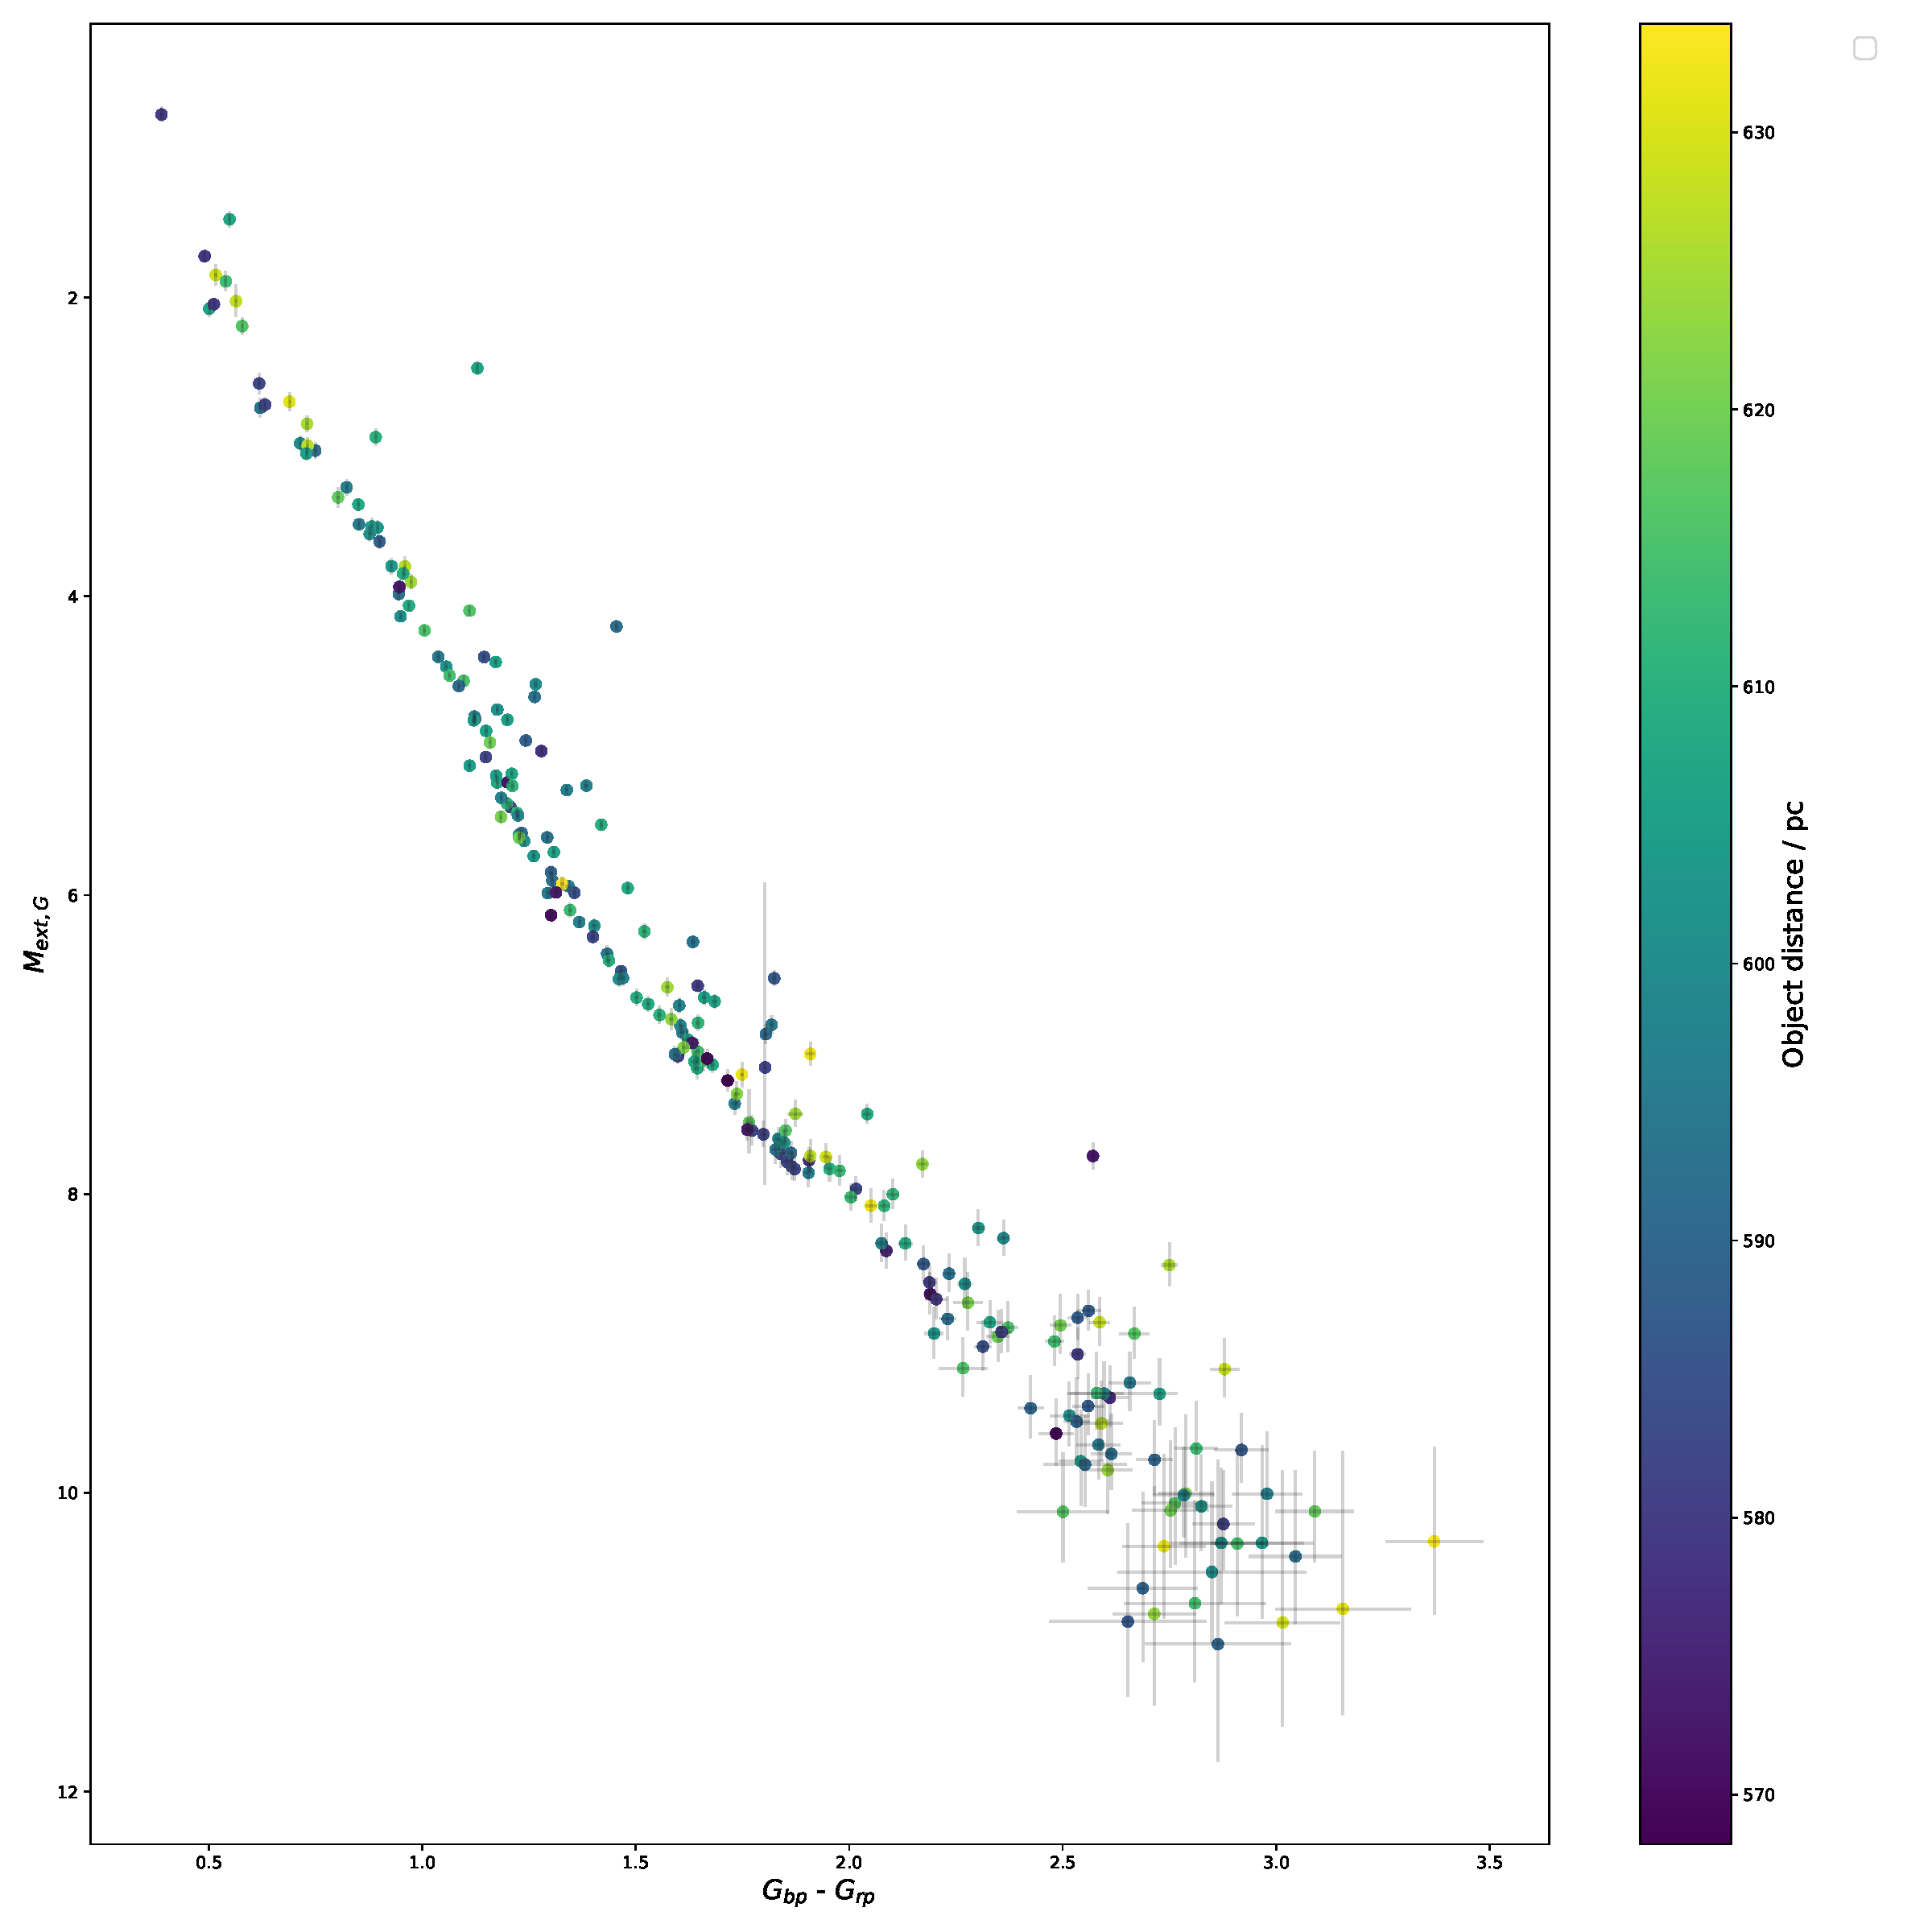
\includegraphics[width=1.0\textwidth]{../NGC_6793_CMD_observational_errorbars_vizier.pdf}
\caption{Gaia $G$-($G_{\textnormal{bp}}$-$G_{\textnormal{rp}}$) CMD of NGC 6793 after the radius selection criterion has been applied. The positions and errors of each object are the same as in Figure \ref{NGC_6793_obs_only_465}, with the only difference being the colour, due to the change in scale of the colour bar shown at the right of the plot.}
\label{NGC_6793_obs_only}
\end{center}
\end{figure}

Therefore, only the radius criterion was implemented, giving 231 objects in the CMD to be analysed, which is smaller than the sample of 271 members used by GC18 for their parameter determination. Figure \ref{NGC_6793_obs_only} shows the results of plotting these 231 members in the Gaia CMD axes. The size and composition of the final dataset adequately reflected both the need for maintaining sufficient data points, to achieve a valid comparison to the previous studies of NGC 6793, particularly GC18, and the need to eliminate the most anomalous stars from the GC18 cluster sample.\\*

The isochrone fitting for NGC 6793 was done by eye using a plot of the cluster's observed Gaia CMD, with the position of each star corrected for its parallax distance. This was chosen over using the measured mean cluster distance for all stars because the parallax-derived photometric errors in the CMD for each star  use the individual parallax measurements and because there is no significant impact on the dataset as a whole, as shown in Figure \ref{indiv_vs_single_distance_check}.\\*

\begin{figure}[h!]
\begin{center}
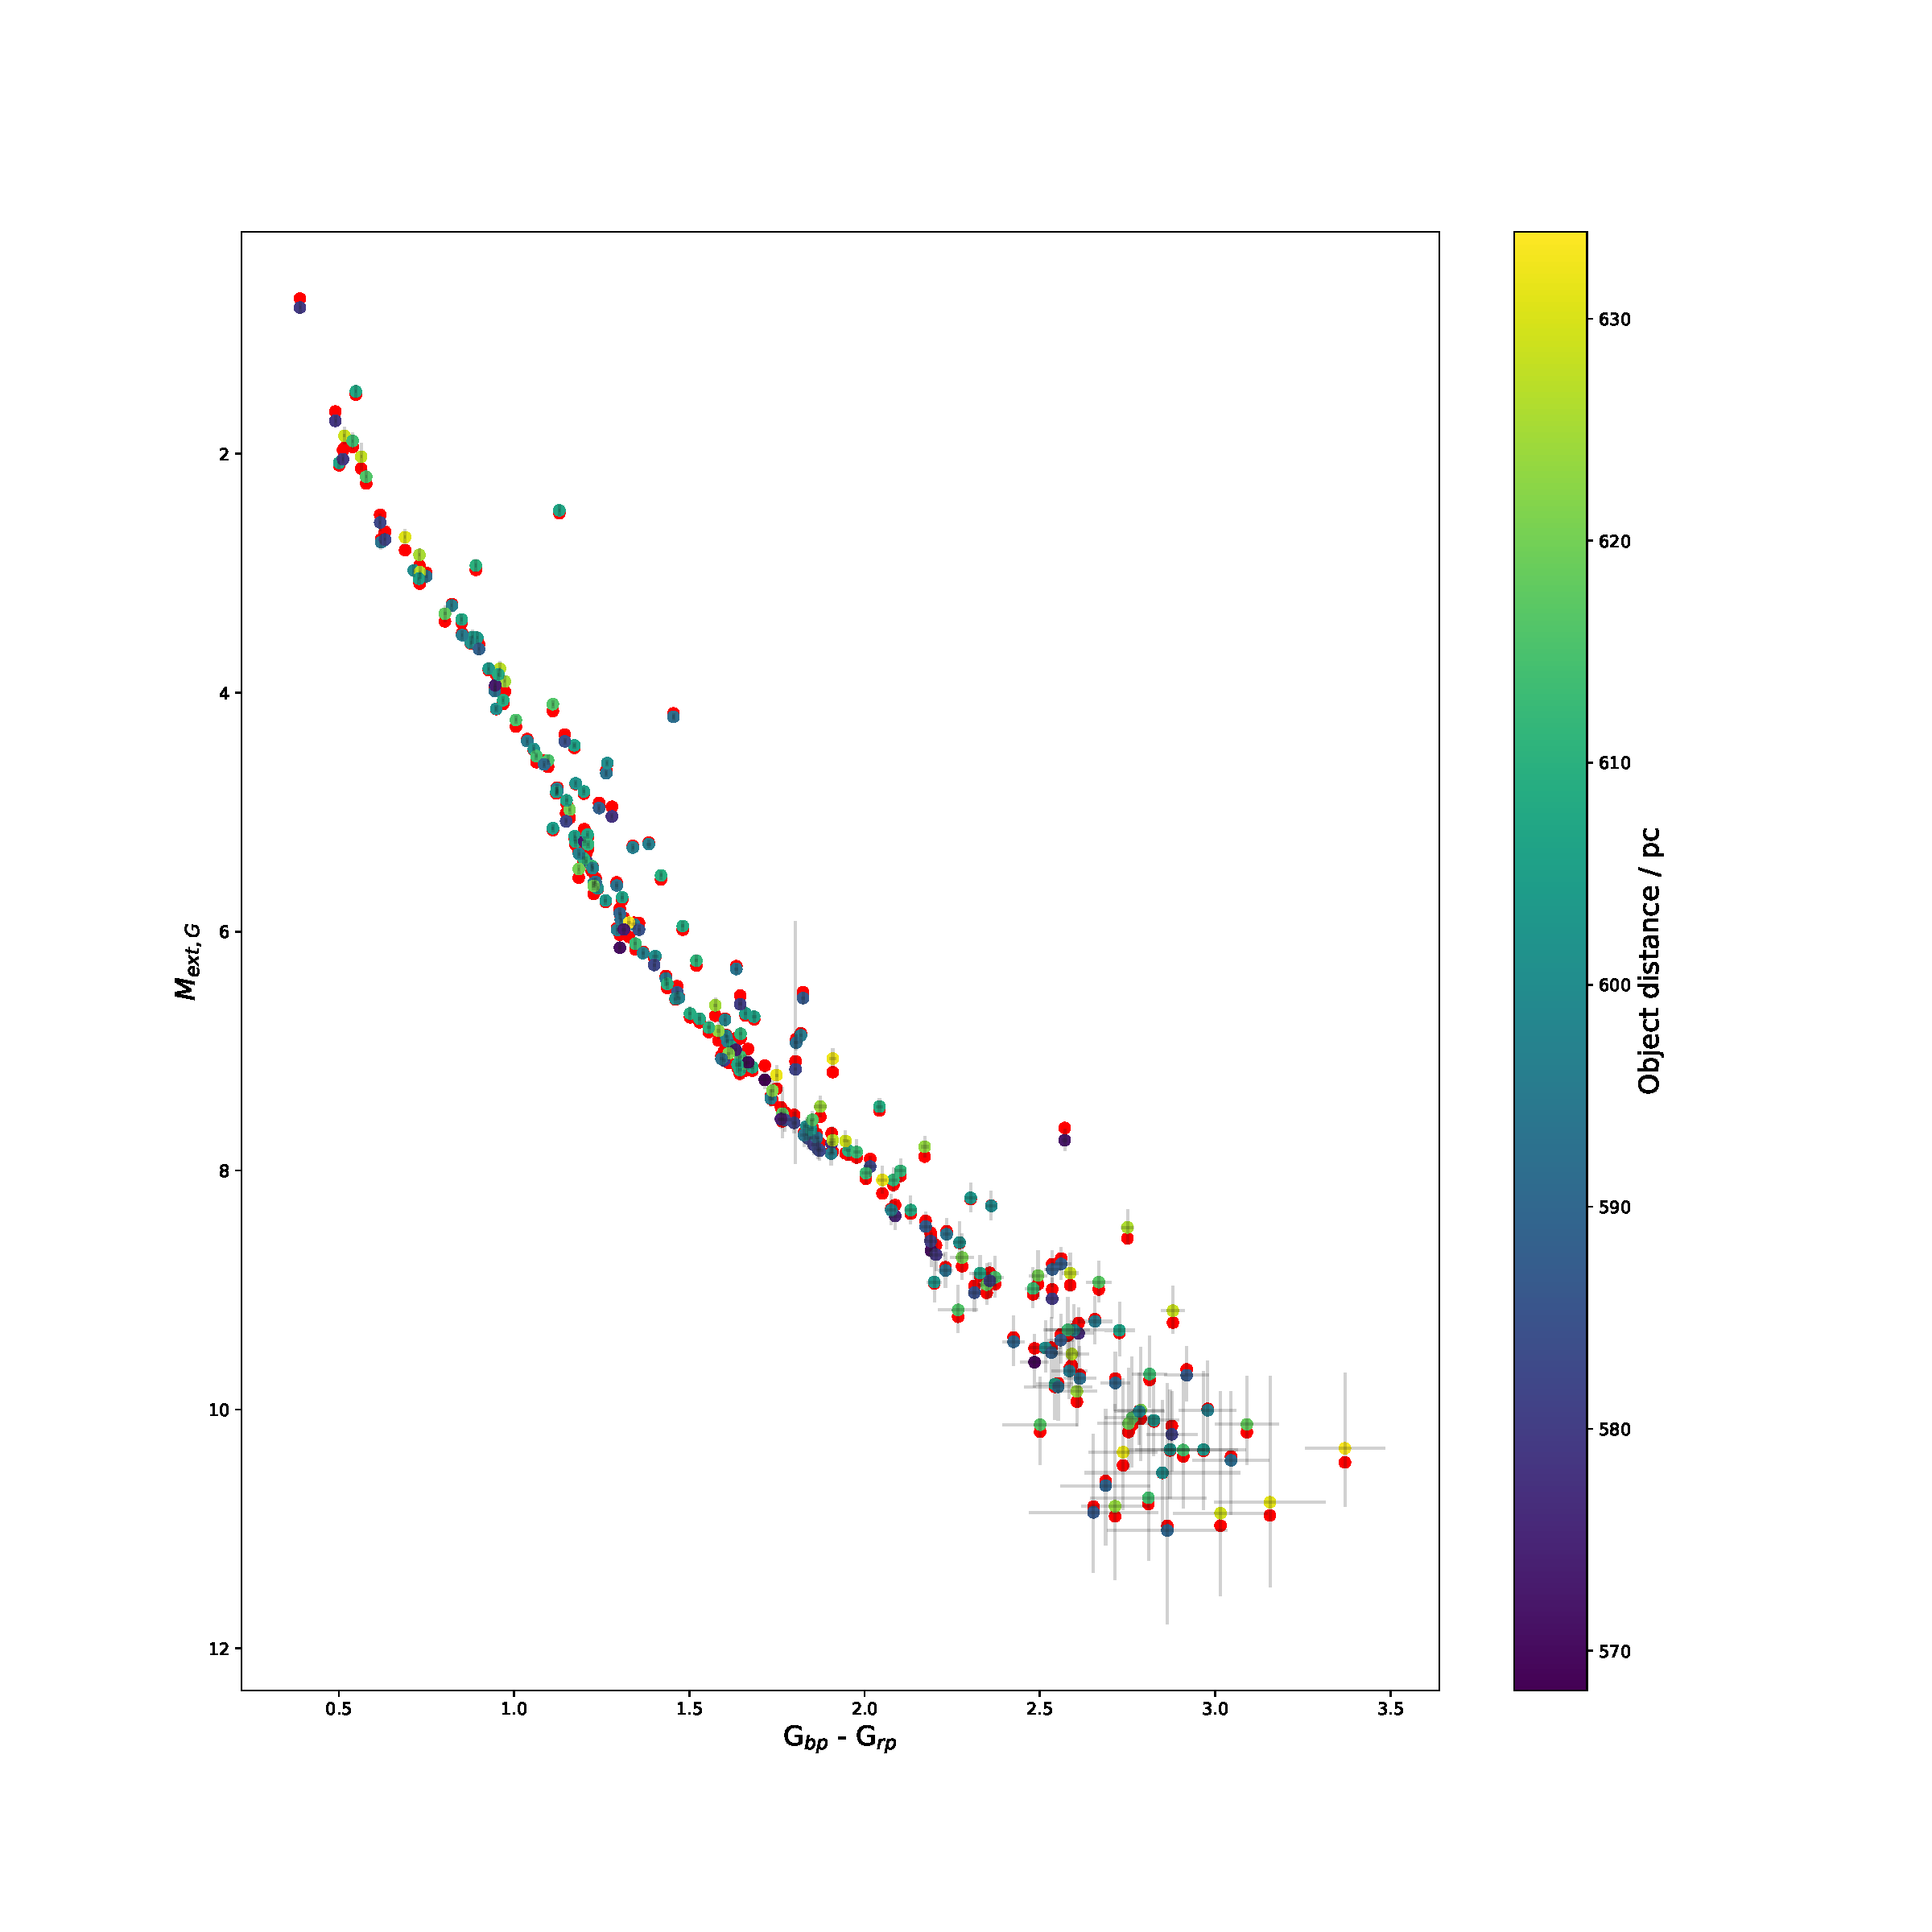
\includegraphics[width=1.0\textwidth]{../NGC_6793_CMD_Myr_single_distance_vizier.pdf}
\caption{Observed CMD of NGC 6793. The distance-coloured points are cluster members whose absolute magnitudes were calculated using their individual parallax-determined observer distances. The red points denote the same data, except that the absolute magnitude were calculated using the GC18 distance value for the cluster for all the stars.}
\label{indiv_vs_single_distance_check}
\end{center}
\end{figure}

Using the values of $E_{B-V}$ and age from GC18, a standard-case isochrone was derived, again assuming a diffuse ISM (i.e., $R_{V} = 3.1$). The standard treatment was employed twice, creating a different isochrone each time. Each time, a different fixed value of $A_{X}/A_{V}$ was used, reflecting the significant changes in the value of $A_{X}/A_{V}$ for different stellar types, as noted in Section \ref{desc_var}. The fitting process was carried out in sequential stages:


\begin{enumerate}
\item First, the upper main sequence of the FBER isochrone below the MSTO region was fitted to that of the fixed-extinction isochrone by varying the value of $A_{V}$ used to calculate the final FBER value for each stellar object.
\item Next, the FBER isochrone metallicity was varied in an attempt match the observed lower main-sequence.
\item Finally, the age of the FBER isochrone was varied to match the observed MSTO location in the NGC 6793 data as far as possible.
\end{enumerate}

It should be noted that, when fitting  to the upper main sequence below the MSTO, priority was given to fainter objects along the line of the MS, as these are most likely to be observations of single stars unaffected by photometrically-unresolved binary companions, making them the most likely to conform to the predictions of stellar evolution models. This is because the effect of an unresolved photometric binary manifests itself as an increase in the flux of the observed star. The size of this increase depends on the ratio of the fluxes emitted by each of the components. The upper limit of this effect is 0.753 magnitudes, equivalent to a doubling of the observed flux, for a binary system composed of two identical stars. The colour index of the unresolved binary, being a difference between two magnitudes, is unaffected. Therefore, binary systems in a given cluster can be identified in a CMD as objects positioned up to 0.753 magnitudes directly above the actual MS and away from, and therefore not associated with, the post-MS regions of the CMD, such as the RGB and AGB. \\*

\begin{figure}[h!]
\begin{center}
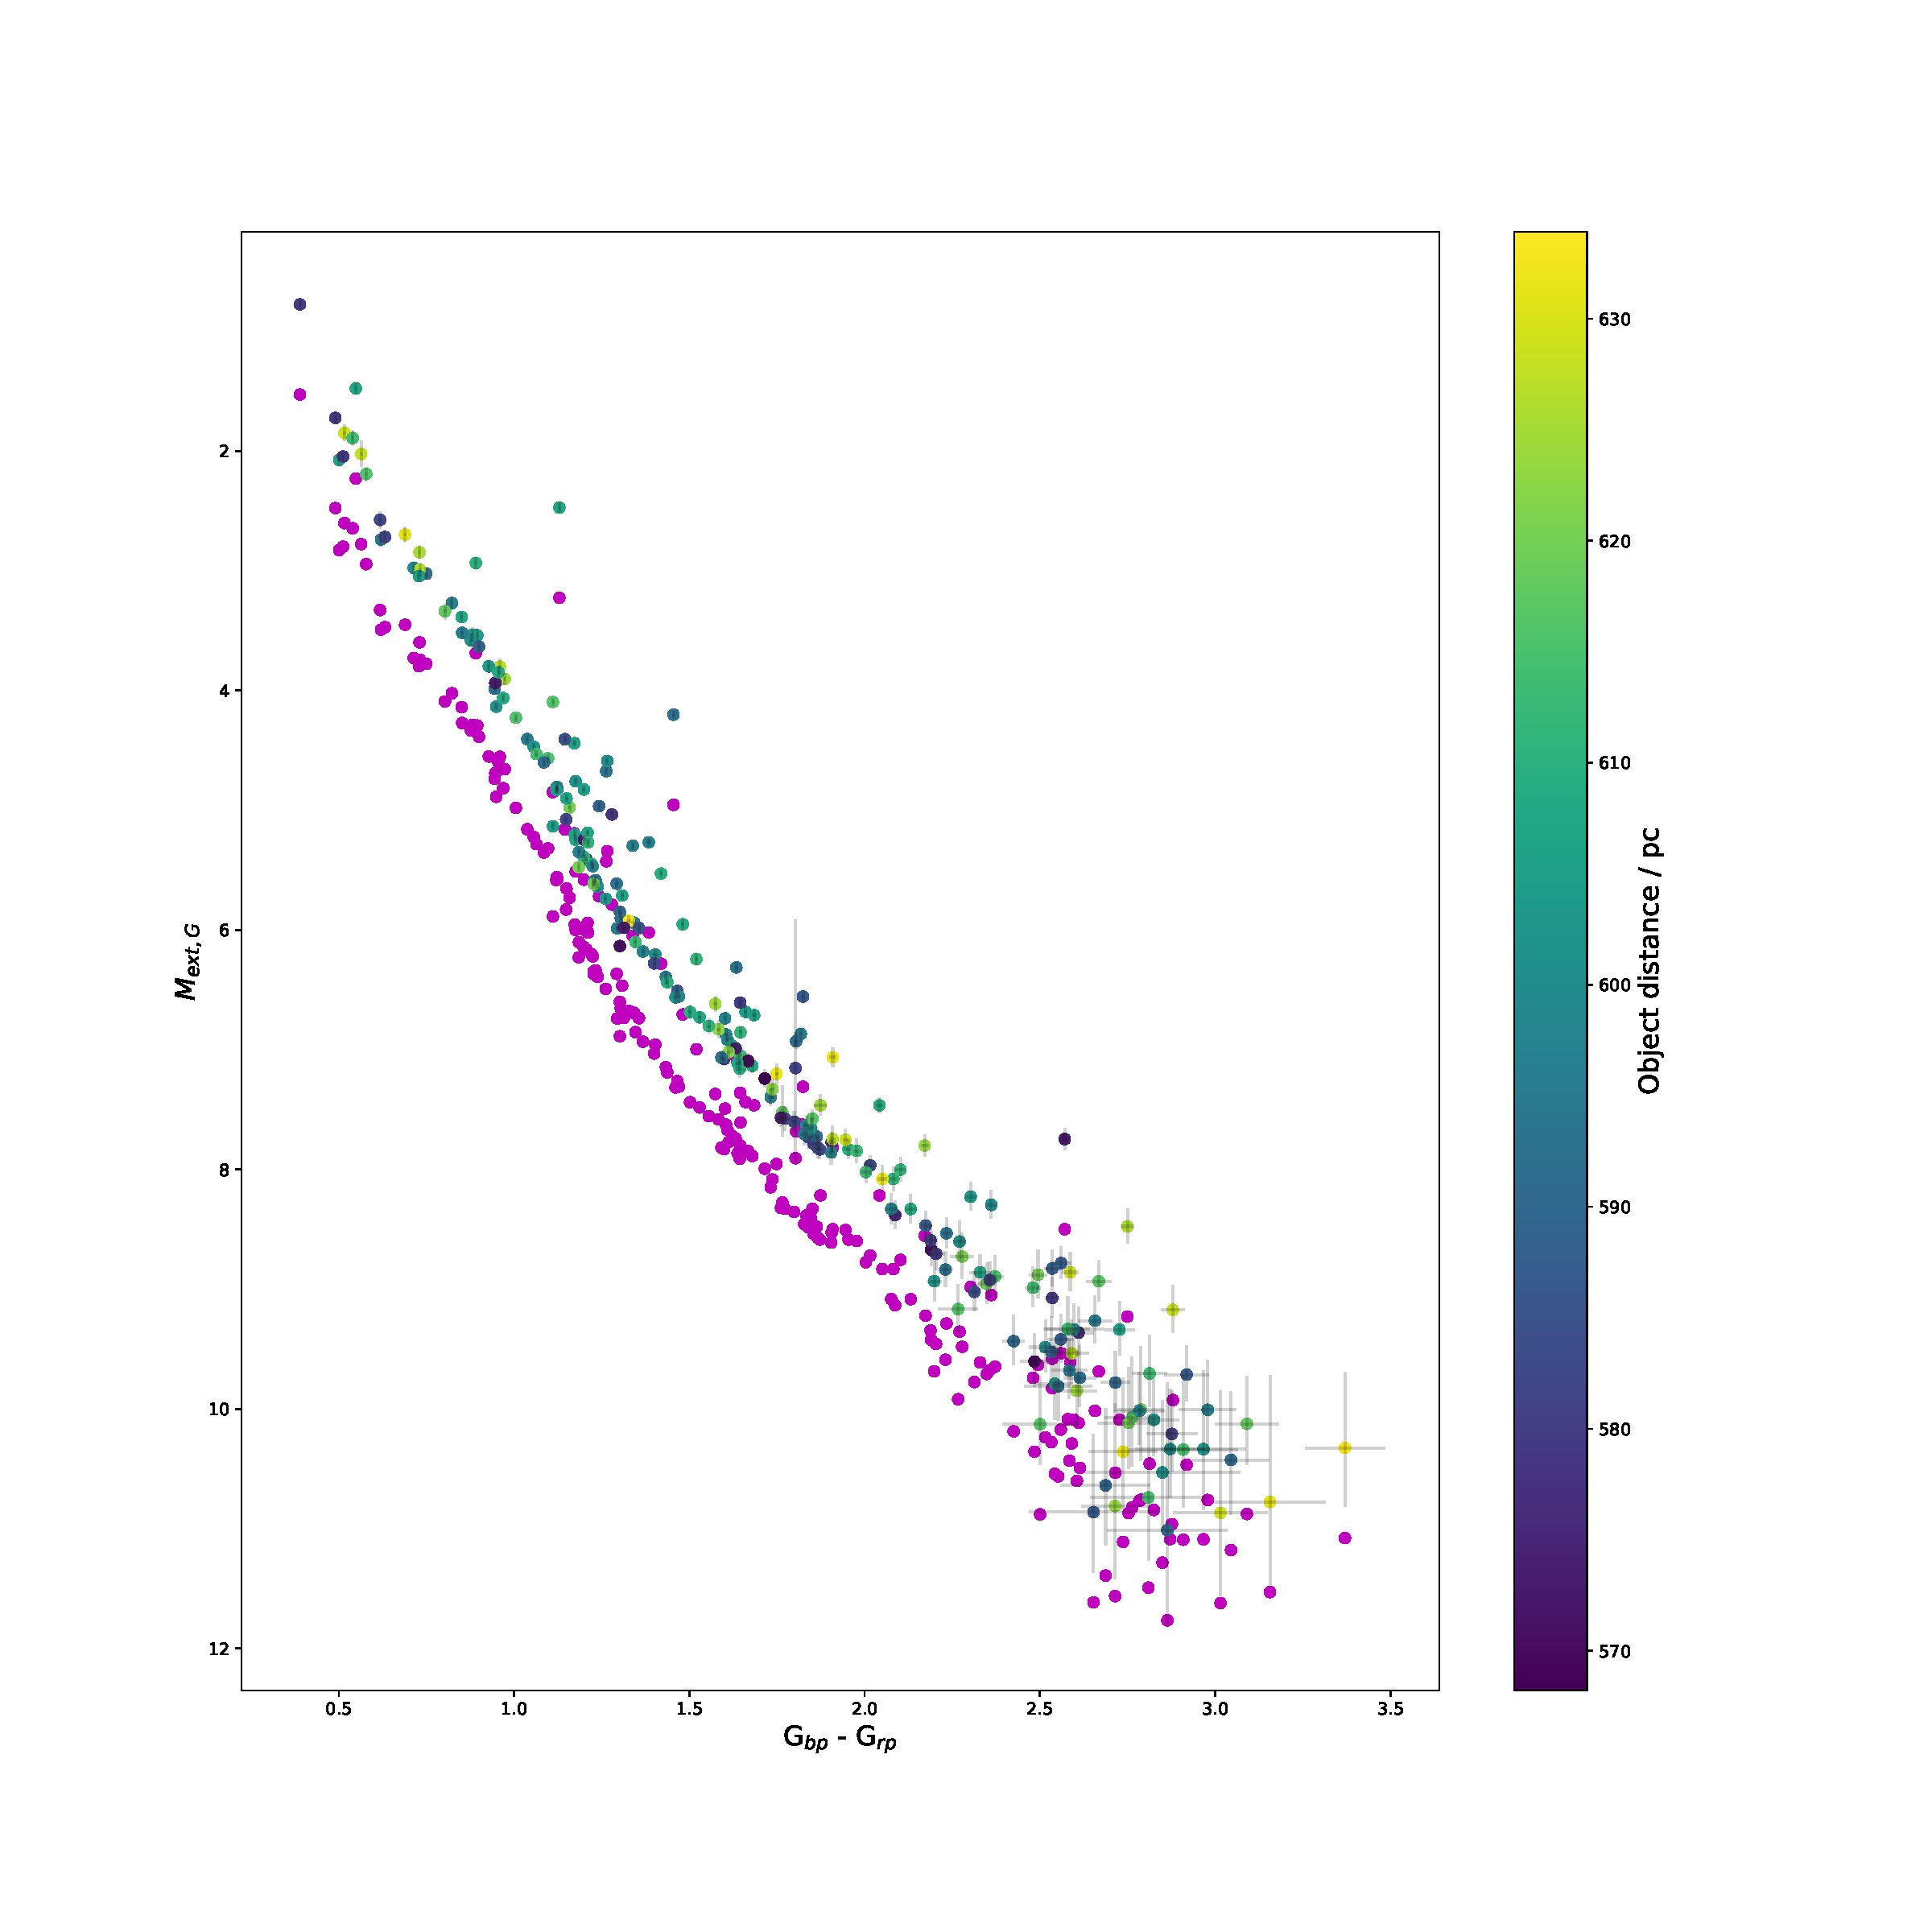
\includegraphics[width=1.0\textwidth]{../NGC_6793_CMD_Myr_binary_check_vizier.pdf}
\caption{The observed CMD of NGC 6793 (coloured by object distance) overplotted with the same data shifted down in the $M_{\textnormal{ext},G}$ direction by 0.753. Purple points which either overlap the observed main sequence or appear between the purple and observed main sequences are likely to represent stars being affected photometrically by flux from unresolved binary companions.}
\label{NGC_6793_binary}
\end{center}
\end{figure}

To illustrate the potential impact on results for NGC 6793 in this project, Figure \ref{NGC_6793_binary} shows the observed CMD data for NGC 6793 plotted twice. The purple points represent the data after they were shifted down by 0.753 magnitudes in the $M_{\textnormal{ext},G}$ direction. From Figure \ref{NGC_6793_binary}, it is clear that only a handful of MS stars have CMD positions which cannot be reconciled to the observed MS under the assumption of an undetected binary companion. Therefore, the use of the faintest MS path was justified on the basis that the vast majority of MS stars that appeared brighter than that path can be easily reconciled with the path by uncertainties caused by potential binary companions.\\*

The isochrone with the resulting parameters was then plotted alongside the two standard-case isochrones. The resulting curves were compared to each other for accuracy with respect to the observational data. In the final stage, the FBER isochrone and the most accurate of the two standard-case isochrone were plotted over the data and their positions and isochrone parameters compared. The results of this are analysed and discussed in Section \ref{ngc6793_res_disc}. \\* 


\section{Software used}
\subsection{Isochrones}
The isochrones used in this project were generated using the latest Bag of Stellar Tracks and Isochrones (BaSTI) web interface \citep{2004ApJ...612..168P,2018ApJ...856..125H}, using the throughput data for all three filter systems analysed in this project. It should be noted that the WFC3 isochrone output for BaSTI does not include flux magnitudes for the F300X filter.\\*

To obtain isochrones from the online database, the desired range of isochrone ages, initial metallicity and photometric filter system must be specified. Therefore, the values of these quantities are shared by all stellar objects in any given isochrone. The output from the BaSTI database for each model stellar object gives the object's initial mass and current mass (i.e. after a time equal to the isochrone age), together with the logarithms of the stellar luminosity in solar units ($\log(L/L_{\odot})$) and of the effective temperature in K ($\log(T_{\textnormal{eff}})$), followed by the predicted absolute magnitudes (with zero extinction) of the object in each filter of the specified filter system. \\*

However, the BaSTI data format for a given isochrone does not include explicit values of the surface gravities or radii of the constituent stars. Therefore, to derive the surface gravity $g$ of a given star, we must combine Equation \ref{Teff_def}, to derive the stellar radius, and Equation \ref{gravity_def}, resulting in the following definition of $g$:

\begin{equation}
\label{gravity_LT_calc}
g = \frac{4 \pi G M_{*} \sigma_{\textnormal{SB}} T_{\textnormal{eff}}^{4}}{L_{*}}
\end{equation}

After this had been completed for all points along an isochrone, each star had a co-ordinate in ($T_{\textnormal{eff}}$, log($g$)) parameter space, plus the metallicity of the overall isochrone model.

\subsection{Stellar atmosphere models}
To generate the predicted stellar flux, pre-calculated ATLAS9 model stellar atmosphere spectra \citep{1993KurCD..13.....K} were employed. The spectra came in the form of tables incorporated wavelengths,ranging from 9 nm to 160,000 nm, with a resolution of 2 nm or less in the UV, and the predicted monochromatic flux at those wavelengths. Each table, representing one stellar spectrum, is identified by the surface gravity, effective temperature and metallicity of the stellar atmosphere producing that spectrum. Table 1 of \cite{2004astro.ph..5087C} contains details of the coverage of the model atmospheres in ($T_{\textnormal{eff}}$, log($g$)) parameter space, while a brief summary  of the limits of the space is listed in Table \ref{atlas9_input}. Four input metallicities were used for ATLAS9, at values of [Fe/H] = -2, -1, 0 and 0.5, covering the metallicities of most observed globular and open clusters. The data for each metallicity value were subject to the same $T_{\textnormal{eff}}$ and log($g$) coverage in ATLAS9.\\*

\begin{table}
\begin{center}
\begin{tabular}{cccc}
\hline
Parameter / unit & Minimum & Maximum & Number of values \\
\hline
$T_{\textnormal{eff}}$ / K & 3500 & 50000 & 76 \\
log( $g$ / cm s$^{-2}$) & 0.0 & 5.0 & 11 \\
$\textnormal{[Fe/H]}$ & -2.0 & 0.5 & 4 \\
\hline
\end{tabular}
\caption{Ranges for the input parameters for ATLAS9 atmospheric models}
\label{atlas9_input}
\end{center}
\end{table}

To make the results of this project apply to the greatest possible range of stellar types, the model atmospheres being employed must ideally be able to reproduce all observed stellar types. Since ATLAS9 atmospheres are constructed from a grid of $T_{\textnormal{eff}}$ and log($g$) values \citep{2004astro.ph..5087C}, the simplest method of ascertaining their applicability is to obtain the widest possible range of $T_{\textnormal{eff}}$ and log($g$) values for the stellar objects which make up the isochrones being employed.\\*

Once the surface gravities for stars in the BaSTI isochrones were calculated via Equation \ref{gravity_LT_calc}, the stars were plotted in ($T_{\textnormal{eff}}$, log($g$)) space onto the grid of co-ordinates for which ATLAS9 spectra were available, as listed in Table 1 of \cite{2004astro.ph..5087C}. The results are shown in Figure \ref{Teff-logg coverage}, using stars in isochrones with ages of 15 Myr (red points) and 15 Gyr (black points). These values are approximately at the available age limits for BaSTI stellar models at [Fe/H] = -1. The blue points represent the ATLAS9 model grid, which extends to the left beyond the $T_{\textnormal{eff}}$-scale presented in the figure, up to a $T_{\textnormal{eff}}$ value of 50,000 K.\\*

\begin{figure}[h!]
\begin{center}
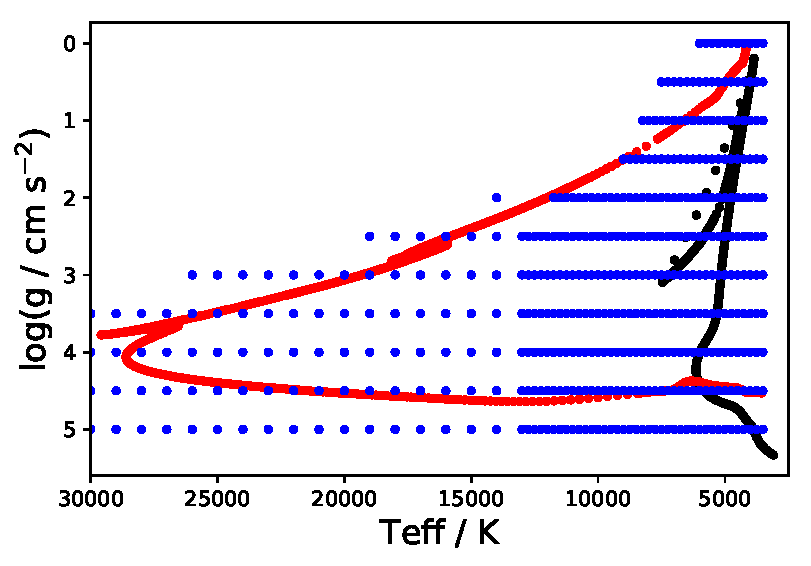
\includegraphics[width=1.0\textwidth]{ATLAS9_grid_BaSTI_coverage_2ages_max.pdf}
\caption{$T_{\textnormal{eff}}$-log($g$) scatter plot for a BaSTI 15 Myr, [Fe/H] = -1 isochrone (red), a BaSTI 15 Gyr, [Fe/H] = -1 isochrone (black) and ATLAS9 model grid (blue) for $T_{\textnormal{eff}} \leq 30000$ K.}
\label{Teff-logg coverage}
\end{center}
\end{figure}

It is clear from Figure \ref{Teff-logg coverage} that the ATLAS9 $T_{\textnormal{eff}}$-log($g$) grid covers the required parameter space for isochrones of all ages including extremely young and extremely old clusters. The only exception to this is the very coolest, and therefore faintest, main sequence stars in the bottom right of the figure. Any changes in the position of the isochrones in the ($T_{\textnormal{eff}}$, log($g$)) plane at the plotted ages due to a change in metallicity were found to have a minimal impact on the overlap between the ATLAS9 grid and both isochrones in the ($T_{\textnormal{eff}}$, log($g$)) plane. Crucially, the MSTO region and the vast majority of the main sequence are both within the region covered by the ATLAS9 grid at all ages and metallicities. \\*

This near-complete coverage of stellar objects in isochrones at all ages allows the ATLAS9 data to be applied to the MSTO locations at all isochrone ages, which ensures the applicability of the best-fit isochrone parameter comparisons described in Section \ref{isoc_fit} to populations of all ages. Therefore, ATLAS9 is a suitable basis from which to begin calculating bolometric corrections and, via Equation \ref{BCs_diff}, extinction ratios. \\*



\subsection{Programming languages}
The tables of bolometric corrections were generated using a FORTRAN 77 code which incorporated Equations \ref{BC_def}-\ref{BCs_diff} and input data files with tables describing the response functions of all relevant filter systems (described in detail in Section \ref{filter_desc}) at the same wavelengths as those listed in the ATLAS9 model atmosphere tables, with the number of tables for each stellar metallicity value equal to the total number of ($T_{\textnormal{eff}}$, log($g$)) combinations available.\\*

Once the bolometric correction tables were produced, all subsequent processes, including the subtraction required to obtain $A_{X}/A_{V}$ shown in Equation \ref{BCs_diff}, were written in Python 2.7 in the form of an IPython notebook. The repository containing all data, plots and programme codes for this project can be found at \protect\url{https://github.com/AlexlwAstro/phd_work}.\\*



\chapter{Results and discussion}
In this chapter, the extinction models resulting from the process described in Section \ref{desc_var} are presented, along with errors in the fitted coefficients and numerical uncertainties in the accuracy of the overall models, in tabulated form. These functions are then implemented to create FBER isochrones, which are compared to isochrones treated with fixed extinction ratios in selected CMDs in all three filter systems. Any differences resulting from these different extinction methods are noted and discussed. Finally, the two methods are applied to the case of NGC 6793. The fixed-extinction isochrone is first aligned with the observational data using the cluster parameters of GC18. The FBER isochrone is aligned with the observational data, with changes in the cluster parameters made as necessary. The results for both isochrones are presented and compared, and the sources of uncertainty for these results are discussed.

\section{Extinction ratio models} \label{ext_models}
In order to find suitable model functions for the $A_{X}/A_{V}$ data in Section \ref{desc_var} without running into issues with degeneracy between coefficients, the relative magnitude of the variations of $A_{X}/A_{V}$ with each of the three parameters became important. Examples of such issues include a coefficient that is multiplied into another, while incorrectly being treated as distinct, in the same function. Degenerate coefficients were identified via two or more coefficients having both apparently plausible values and abnormally high standard deviations. Plausible values were determined to be values which were not at the limits or midpoint of the acceptable range set prior to fitting and which were produced consistently over many fitting iterations. If, upon further investigation, these coefficients were found to contribute to the same attribute of the overall function, the function was rewritten to combine the relevant coefficients into one describing the same attribute.\\*

This resulted in relatively simple functions expressed solely in terms of $T_{\textnormal{eff}}$, which caused the greatest variations, to be fitted first. The coefficients resulting from the fitting process were then incorporated into the function to form a predicted $A_{X}/A_{V}$ model of $T_{\textnormal{eff}}$ in each filter. The residuals generated by the subtraction of this predicted model from the original data could then be examined for any significant disagreements between the data and these simple models and for any further variations with log($g$) or [Fe/H]. This allowed functions to be constructed incrementally, with a lower risk of becoming overly complex - too many coefficients would create errors that were significantly greater in degenerate coefficients than in non-degenerate ones, which would obscure any useful information about the validity of the function form. \\*

The fitting operation for the initial functions of $T_{\textnormal{eff}}$ was carried out on the dataset for solar metallicity ([Fe/H] = 0.0) ATLAS9 atmospheres and, because it gave the greatest number of $T_{\textnormal{eff}}$ data points, log($g$) = 5.0. As mentioned in Section \ref{desc_var}, due to the difficulties posed by the tail-flick phenomenon in certain filters, when fitting for $A_{\textnormal{pow}}$ and $A_{\textnormal{exp}}$, the lower $T_{\textnormal{eff}}$ limit for the fitting data was set at 4500K for all filters. This dataset will be referred to as the basic fitting data (BFD). The first functions to be fitted to the BFD had the following forms:

\begin{equation}
A_{\textnormal{pow}} = \left(\frac{A_{X}}{A_{V}}\right)_{\textnormal{pow}}(T_{\textnormal{eff}}) = a (T_{4})^{b} + c
\label{Teff_pow}
\end{equation}

\begin{equation}
A_{\textnormal{exp}} = \left(\frac{A_{X}}{A_{V}}\right)_{\textnormal{exp}} (T_{\textnormal{eff}}) = a \exp(b T_{4}) + c
\label{Teff_exp}
\end{equation}
where $T_{4} = 10^{-4} \times T_{\textnormal{eff}}$ and $a$,$b$ and $c$ are coefficients. These functions were fitted separately to the BFD for each filter and compared both visually and via the size of the residuals. The most accurate function form was then selected as the final form. The results of this fitting process are detailed, for the cases where the either the $A_{\textnormal{exp}}$ or the $A_{\textnormal{pow}}$ fitting result was sufficiently accurate, in Table \ref{simpfunc_coeffs_table}. The table shows the filters and lists which of the two functions provided the best fit for the relevant data, followed by the respective coefficient values and the associated uncertainties. Due to the fitting data being restricted to atmospheres with $T_{\textnormal{eff}}$ values greater than 4500K, the models could not simply be assumed to apply to cooler atmospheres as well. The penultimate column in Table \ref{simpfunc_coeffs_table} lists the lowest $T_{\textnormal{eff}}$ value for which the given combination of coefficient values is valid at all combinations of surface gravity and metallicity, denoted by $T_{\textnormal{min}}$. The final column shows the maximum deviation of the extinction ratio model from the data, over all stellar atmospheres with $T_{\textnormal{eff}} \geq T_{\textnormal{min}}$, including those not in the BFD (i.e, at non-solar metallicities and lower surface gravities). \\*


\begin{table}
\begin{center}
\resizebox{\textwidth}{!}{\begin{tabular}{cccccccc}
\hline
\multirow{2}{*}{System} & \multirow{2}{*}{Filter} &  Function & & Coefficients & & \multirow{2}{*}{$T_{\textnormal{min}}$ / K} & \multirow{2}{*}{Max. deviation in $A_{X}/A_{V}$} \\
 & & ($A_{\textnormal{pow}}$ or $A_{\textnormal{exp}}$) & $a$ & $b$ & $c$ & & \\
\hline
& F435W & exp & -0.1436$\pm$0.0310 & -2.159$\pm$0.360 & 1.352$\pm$0.002 & 3500 & 0.03 \\
& F475W & exp & -0.2137$\pm$0.0469 & -2.660$\pm$0.380 & 1.226$\pm$0.002 & 4000 & 0.03 \\
& F555W & exp & -0.0914$\pm$0.0476 & -2.677$\pm$0.901 & 1.045$\pm$0.002 & 3500 & 0.01 \\
ACS & F606W & exp & -0.2183$\pm$0.0554 & -2.867$\pm$0.445 & 0.959$\pm$0.002 & 3500 & 0.01 \\
& F625W & exp & -0.0719$\pm$0.0798 & -3.332$\pm$2.000 & 0.865$\pm$0.002 & 3500 & 0.01 \\
& F775W & pow & -0.0035$\pm$0.0042 & -1.488$\pm$1.541 & 0.651$\pm$0.003 & 3500 & 0.01 \\
& F814W & pow & -0.0070$\pm$0.0046 & -1.374$\pm$0.830 & 0.611$\pm$0.003 & 3750 & 0.02 \\ \hline

& F336W & pow & -0.0074$\pm$0.0041 & -1.525$\pm$0.727 & 1.648$\pm$0.003 & 3500 & 0.03 \\
& F390W & exp & -0.0695$\pm$0.0057 & -0.644$\pm$0.177 & 1.489$\pm$0.005 & 4500 & 0.04 \\
& F438W & exp & -0.1132$\pm$0.0658 & -3.084$\pm$1.032 & 1.350$\pm$0.002 & 3750 & 0.02 \\
& F475W & pow & -0.0179$\pm$0.0037 & -1.718$\pm$0.275 & 1.220$\pm$0.003 & 4000 & 0.02 \\
WFC3 & F555W & pow & -0.0138$\pm$0.0033 & -1.887$\pm$0.333 & 1.080$\pm$0.003 & 3750 & 0.02 \\
& F606W & exp & -0.2131$\pm$0.0559 & -2.879$\pm$0.460 & 0.962$\pm$0.002 & 3500 & 0.02 \\
& F625W & pow & -0.0042$\pm$0.0031 & -2.063$\pm$1.025 & 0.879$\pm$0.002 & 3500 & 0.01 \\
& F775W & pow & -0.0033$\pm$0.0041 & -1.529$\pm$1.634 & 0.657$\pm$0.003 & 3750 & 0.01 \\
& F814W & pow & -0.0071$\pm$0.0046 & -1.391$\pm$0.803 & 0.616$\pm$0.004 & 4000 & 0.01 \\ \hline

& G & pow & -0.0888$\pm$0.0045 & -1.402$\pm$0.064 & 1.040$\pm$0.004 & 4000 & 0.02 \\
Gaia & G\textsubscript{bp} & pow & -0.1150$\pm$0.0081 & -0.900$\pm$0.070 & 1.247$\pm$0.007 & 3750 & 0.03 \\
& G\textsubscript{rp} & pow & -0.0159$\pm$0.0047 & -1.352$\pm$0.368 & 0.677$\pm$0.004 & 3750 & 0.02 \\ \hline

\end{tabular}}
\caption{Coefficient values produced for each filter via $A_{\textnormal{exp}}$ or $A_{\textnormal{pow}}$ fitting, as appropriately labelled. Any filters missing from this table are those with data that could not be accurately fitted using either function. The errors are calculated using an acceptable 1$\sigma$ margin, $\Delta(A_{X}/A_{V})$, of 0.01. The penultimate column ($T_{\textnormal{min}}$) displays the lowest effective temperature, including for atmospheres outside the BFD, for which the given model and coefficients were able to describe the $A_{X}/A_{V}$ data across all values of log($g$) and [Fe/H] to a level of accuracy within the deviation shown in the final column.}
\label{simpfunc_coeffs_table}
\end{center}
\end{table}

For the wide-field WFC3, ACS and Gaia \citep{2014MNRAS.444..392C,2018MNRAS.479L.102C} filters that were examined in the relevant studies, the opportunity was taken to compare the models for $R_{X} = (A_{X}/E_{B-V})$ calculated in those studies, whose basic form is shown in Equation \ref{casagrande_ext_fit}, with the $A_{X}/A_{V}$ data calculated in this project for the same filters. To perform this comparison, it is necessary to define $A_{X}/A_{V}$ explicitly in terms of $R_{X}$. Using the definitions of $R_{X}$ and $R_{V}$, this can be done via the following equation:

\begin{equation}
\frac{A_{X}}{A_{V}} = \frac{R_{X}}{R_{V}} = \frac{R_{X}}{3.1}
\label{convert_Rx_to_Ax}
\end{equation}
The $R_{X}$ models, when modified in this way to produce predictions of $A_{X}/A_{V}$ values, consistently underestimate the $A_{X}/A_{V}$ values listed in the data for atmospheres at log($g$) = 4.0 (the $R_{X}$ models used atmospheric data with log($g$) = 4.1) in this project in almost all filters. However, within the metallicity and temperature ranges for which these $R_{X}$ models are applicable (detailed in Section \ref{empirical}), they remain in agreement with the data to within a deviation in $A_{X}/A_{V}$ of 0.03, which is a similar level of accuracy to that achieved by the $A_{X}/A_{V}$ functions produced in this project for the same filters. Therefore, it was surmised that both these $R_{X}$ models and the models listed in Table \ref{simpfunc_coeffs_table} are consistent with the ATLAS9-derived extinction ratio data.\\*

There were filters, namely the four WFC3 filters with the shortest central wavelengths (F218W,F225W, F275W and F300X), for whose BFD neither $A_{\textnormal{pow}}$ nor $A_{\textnormal{exp}}$ was able to produce an accurate fit across all combinations of log($g$) and [Fe/H]. For these filters, more intricate functions were sought, including functions with explicit dependences on $g$ and [Fe/H]. Several unsuccessful attempts were made before an acceptable function was found for these filters.\\*

The most successful approach for these filters involved plotting all the available $A_{X}/A_{V}$ data for each filter, in all possible 2D and 3D axis combinations, and analysing it visually. The trends seen in the data were analysed to determine both a basic overarching function for the extinction ratio and further mathematical functions (referred to hereafter as ``sub-functions'') to describe the parameters in the overarching function. Examples of sub-functions are given in Equations \ref{T0_eq} and \ref{decay_const_eq}, with the relevant overarching function given in Equation \ref{A_logis_UV}.\\*

\begin{figure}[h!]
\begin{center}
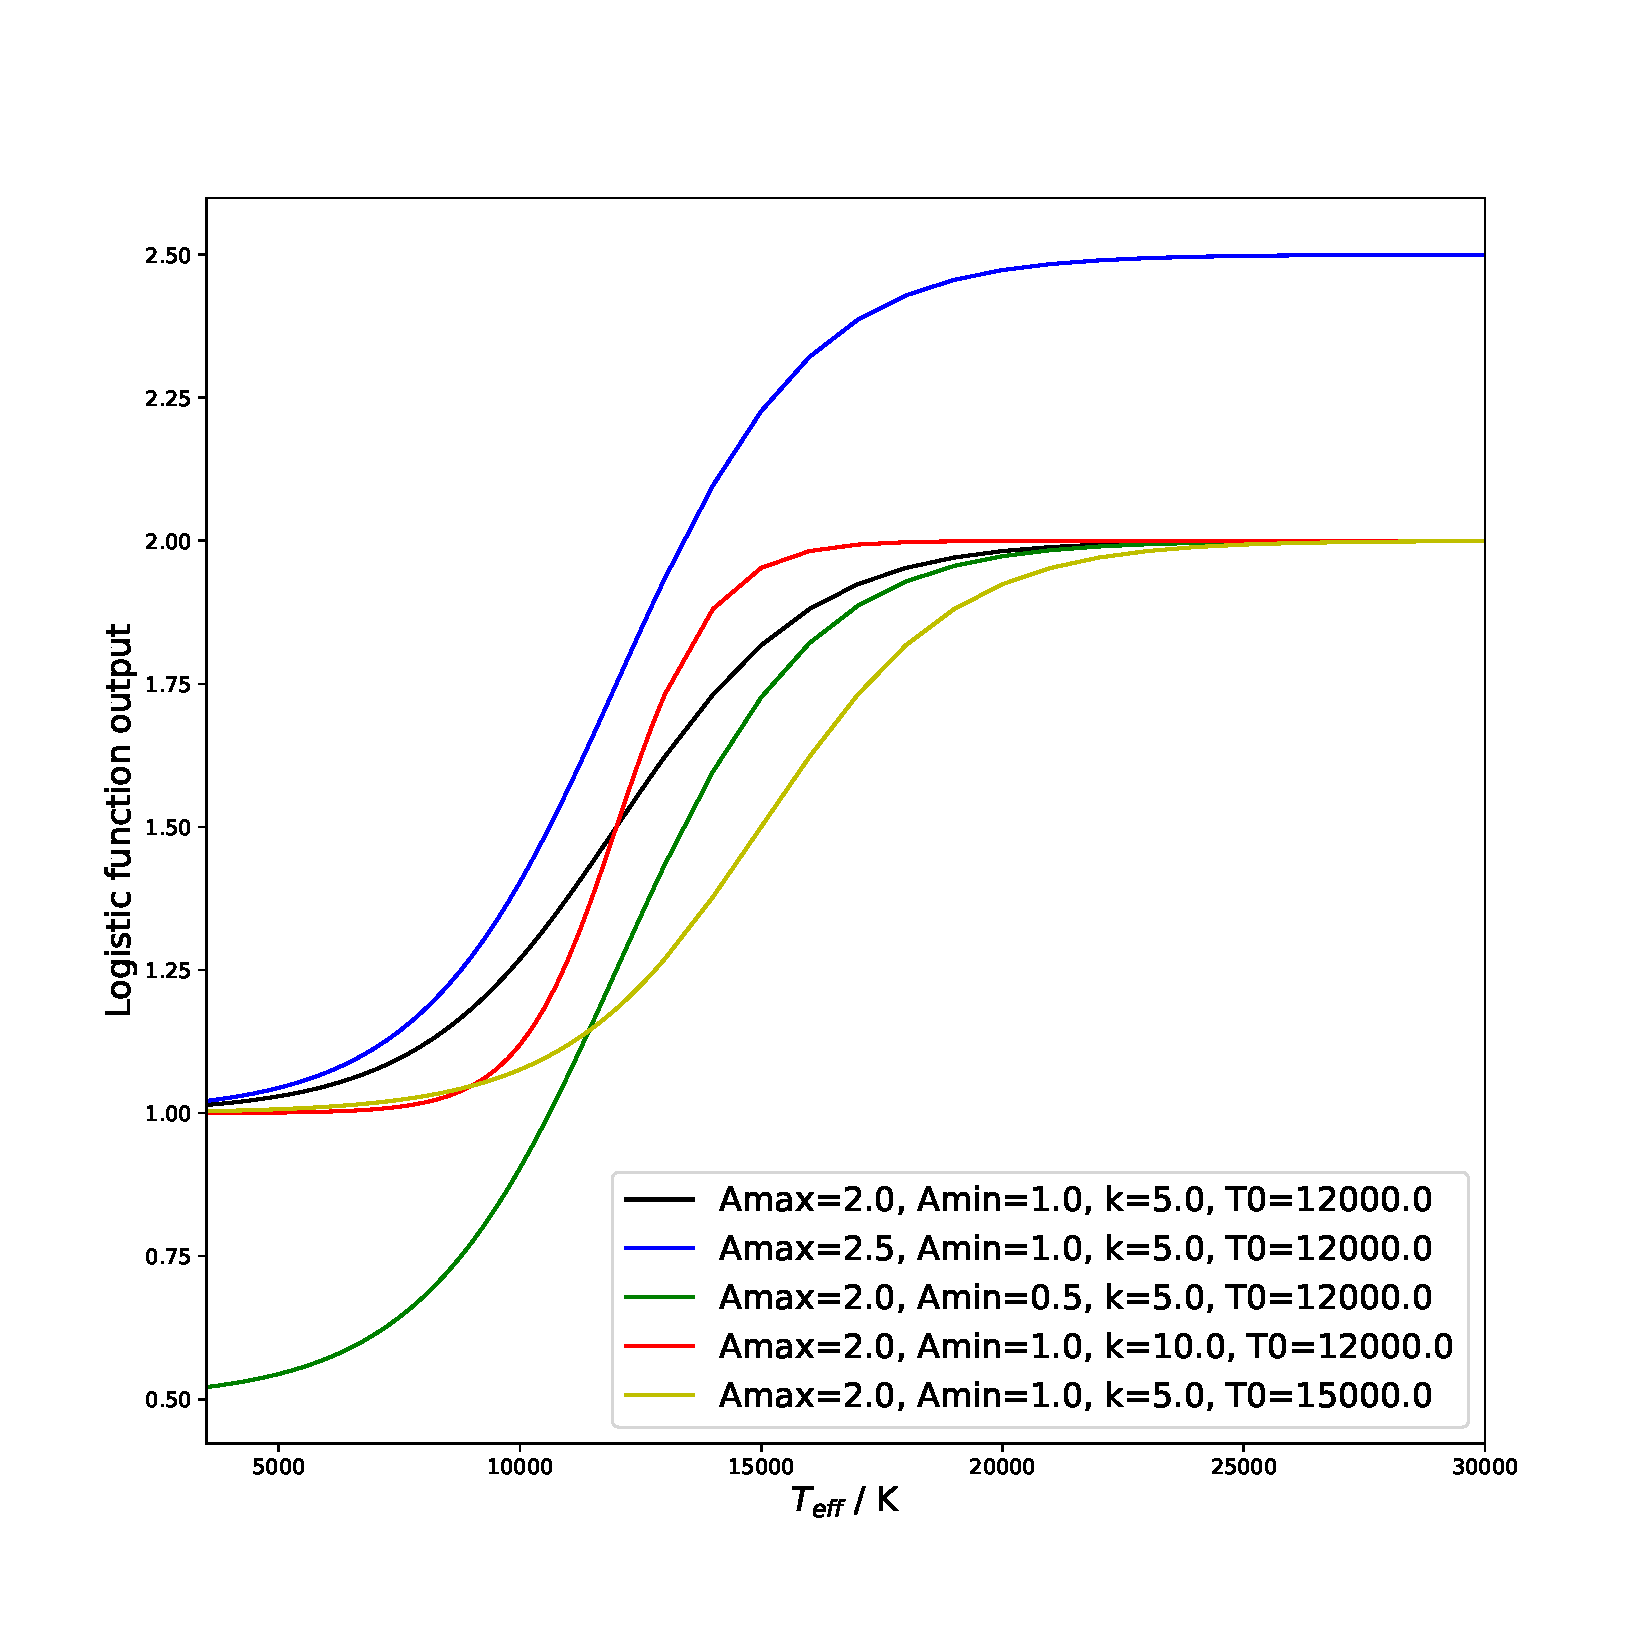
\includegraphics[width=1.0\textwidth]{generic_logistic_params_illustration.pdf}
\caption{Plots of several generic logistic functions, all described by the four parameters ($A_{max}$, $A_{min}$, $k$, $T_{\textnormal{0}}$) listed in the text. Each curve illustrates the effect of changing the value of one parameter, as detailed in the legend, from the values listed for the black curve.}
\label{logistic_curve_example}
\end{center}
\end{figure}

The details of the final form of the functions for these filters, including dependences on any of the stellar parameters, were deduced by fitting a logistic function of $T_{\textnormal{eff}}$ to the $A_{X}/A_{V}$ data for each ([Fe/H],log($g$)) combination. This was chosen on the basis that $A_{\textnormal{exp}}$ had been superior to $A_{\textnormal{pow}}$ in describing the data for these particular filters and because the low-$T_{\textnormal{eff}}$ change in gradient appeared to be more significant than for other filters. Furthermore, the gradient was not inverted, as can be seen in Figure \ref{just_data_FeH0_WFC3gaia}, thus avoiding any tail-flick complications. Of particular importance was the additional fact that the steep $T_{\textnormal{eff}}$ gradient in the region between the shallow low-$T_{\textnormal{eff}}$ gradient and the plateau appears to lead to an asymptote at lower stellar effective temperatures, if the shallower low-$T_{\textnormal{eff}}$ gradient is ignored when constructing and fitting a function (as was done for both $A_{\textnormal{exp}}$ and $A_{\textnormal{pow}}$). In these four filters, this steep gradient was found to cause functions such as $A_{\textnormal{exp}}$ and $A_{\textnormal{pow}}$ to predict negative values of the extinction ratio at $T_{\textnormal{eff}}$ values that were still above the lowest values derived from observations of cool stars (excluding brown dwarfs). This issue is resolved by the logistic function's property of converging to a constant value for both high and low values of $T_{\textnormal{eff}}$. Therefore, for these filters, the data to which the functions were fitted encompassed all available $T_{\textnormal{eff}}$ values down to the ATLAS9 minimum of 3500K. For a general logistic function in $T_{\textnormal{eff}}$ (whose basic form is shown in Equation \ref{A_logis_UV}), there are four key parameters:

\begin{itemize}
\item The global maximum value, denoted in this case by $A_{max}$;
\item The global minimum value, $A_{min}$;
\item The exponential decay coefficient, $k$;
\item The $T_{\textnormal{eff}}$-coordinate of the midpoint of the characteristic S-shape, or sigmoid, of the logistic curve function curve, in this case $T_{\textnormal{0}}$.
\end{itemize}

Figure \ref{logistic_curve_example} shows a plot of five generic logistic curves of $T_{\textnormal{eff}}$ described by the four parameters listed above, with the black curve used as a starting point and each of the other four curves resulting from changing one of the four parameter values of the black curve, as detailed in the legend. Changing the values of $A_{min}$ (blue curve) and $A_{max}$ (green curve) change the maximum and minimum of the function output, respectively, when compared to the black curve. Increasing the $k$ value (red curve) causes a more rapid exponential decay between $A_{min}$ and $A_{max}$ and, by doing so, effectively reduces the $T_{\textnormal{eff}}$ range within which output values change. Increasing the value of $T_{\textnormal{0}}$ (yellow curve) shifts the entire black curve to the right of the plot without changing its shape. Looking at $A_{X}/A_{V}$ data for the four relevant WFC3 filters in Figure \ref{just_data_FeH0_WFC3gaia}, it is apparent that while some of the logistic parameters, such as $A_{max}$, can be taken as constant for all combinations of log($g$) and [Fe/H], others, such as $T_{\textnormal{0}}$. The relevant curves in Figure \ref{just_data_FeH0_WFC3gaia} show that as log($g$) decreases, the $A_{X}/A_{V}$ midpoint of the curve occurs at progressively higher $T_{\textnormal{eff}}$ - meaning that $T_{\textnormal{0}}$ must replicate this behaviour in the models. A similar pattern occurs when analysing the behaviour of $A_{X}/A_{V}$ with varying metallicity in the same filters. \\*

It was confirmed that this logistic function of $T_{\textnormal{eff}}$ could describe the $A_{X}/A_{V}$ variations accurately in each filter for every combination of atmospheric log($g$) and [Fe/H] values, using the four parameters listed above. This was done numerically by fitting the logistic function to the $A_{X}/A_{V}$ data for each (log($g$),[Fe/H]) combination individually. The values produced for the four coefficients of the logistic function listed above for each of these fits were tabulated along with the log($g$) and [Fe/H] values of their respective datasets. This table was then analysed for trends in the values for all four coefficients as log($g$) and [Fe/H] were varied. This allowed for the incremental construction, where necessary, of sub-functions to describe the parameters of the main $T_{\textnormal{eff}}$ logistic function in terms of log($g$) and [Fe/H].\\*

Many different forms, of varying complexity, were tested for these sub-functions by incorporating each form into the principal $T_{\textnormal{eff}}$-logistic function. In some cases, sub-functions with explicit $T_{\textnormal{eff}}$ dependences were included. The resulting function was then subjected to a single fit on the entire $A_{X}/A_{V}$ dataset, covering the entire ($T_{\textnormal{eff}}$,  log($g$), [Fe/H]) parameter space available. The suitability of each function was influenced by both the size of the $A_{X}/A_{V}$ residuals and on the relative errors on the coefficients resulting from the fit. The importance of the latter was due to multiple factors:

\begin{itemize}
\item the possibility of degeneracies between coefficients being overlooked during the construction of either the sub-functions, the overall logistic function or both, which would result in anomalously high errors for the relevant coefficients;
\item the possible occurrence of a near-zero best-fit value for a given coefficient with a high associated error, indicating that the coefficient was describing a trend not actually present in the data and that, therefore, the overall function was overly complex;
\item the possibility of coefficient values not departing from their starting value with a listed output error of zero, indicating that, for that coefficient, the algorithm was unable to achieve convergence, even after a very large number of iterations, and defaulted to the starting value.
\end{itemize}

The best form for the sub-functions which represented $T_{0}$ and $k$ in each filter were found to be simple functions of log($g$) and [Fe/H], independent of $T_{\textnormal{eff}}$ variations, as shown in Equations \ref{T0_eq} and \ref{decay_const_eq}, respectively. It was found that $A_{min}$ and $A_{max}$ were best expressed as constants for each filter. The overall function, $A_{\textnormal{logis}}$, shown in Equation \ref{A_logis_UV}, is therefore sensitive to all three input stellar atmosphere parameters, with effective temperature having the greatest effect and the other parameters having much smaller but still significant effects, with the relative magnitudes dependent on the values of the associated coefficients.\\*


\begin{sidewaystable}
\begin{center}
\resizebox{\textwidth}{!}{\begin{tabular}{cccccccccc}
\hline
\multirow{2}{*}{Filter} & \multicolumn{8}{c}{Coefficient} & Global max. \\
 & $a$ & $b$ & $c$ & $d$ & $e$ & $f$ & $A_{min}$ & $A_{max}$ & deviation in $A_{X}/A_{V}$\\
\hline
F218W & -120.9$\pm$4.1 & 467.6$\pm$7.9 & 5673$\pm$16 & 1.435$\pm$0.209 & -3.211$\pm$0.382 & 19.19$\pm$0.62 & 1.026$\pm$0.012 & 2.909$\pm$0.003 & 0.25 \\
F225W & -97.21$\pm$3.85 & 357.2$\pm$7.9 & 4967$\pm$22 & -0.174$\pm$0.136 & -2.691$\pm$0.256 & 18.62$\pm$0.55 & 0.337$\pm$0.028 & 2.581$\pm$0.003 & 0.3 \\
F275W & -239.0$\pm$12.0 & 236.0$\pm$20.4 & 4161$\pm$79 & -2.117$\pm$0.326 & -2.140$\pm$0.445 & 22.20$\pm$1.48 & 0.409$\pm$0.113 & 2.030$\pm$0.003 & 0.2 \\
F300X & -302.1$\pm$45.0 & 350$\pm$125 & 4270$\pm$913 & -0.176$\pm$0.087 & -0.352$\pm$0.115 & 4.315$\pm$0.529 & 1.000$\pm$0.199 & 2.015$\pm$0.004 & 0.15 \\
\hline

%($T_{\textnormal{eff}}$ / K, & & & None & None \\
%log($g$) / dex, & & & None & None \\
%$\textnormal{[Fe/H]}$) & & & None & None \\
%exceptions & & & & \\
\hline
\end{tabular}}
\caption{Coefficient values for the non-trivial $A_{X}/A_{V}$ function $A_{\textnormal{logis}}$, described in Equations \ref{T0_eq}-\ref{A_logis_UV}, produced by fitting to UV filter data with The errors are calculated using an acceptable 1$\sigma$ margin, $\Delta(A_{X}/A_{V})$, of 0.1. The bottom row represents the maximum deviation from the data across the entire ($T_{\textnormal{eff}}$, log($g$), [Fe/H]) parameter space. All results are valid down to $T_{\textnormal{eff}}$ = 3500 K.}
\label{UV_coeffs_table}
\end{center}
\end{sidewaystable}

This final form of $A_{\textnormal{logis}}$ was able to accurately reproduce the behaviour of almost the entire dataset. The coefficients for Equations \ref{T0_eq}-\ref{A_logis_UV} are given in Table \ref{UV_coeffs_table}.

\begin{align}
T_{\textnormal{0}} &= a\log(g) + b\left(\frac{\left[\textnormal{Fe/H}\right]}{\left|\left[\textnormal{Fe/H}\right]\right|^{1/2}}\right) + c \label{T0_eq}\\
k &= d\log(g) + e\left[\textnormal{Fe/H}\right] + f \label{decay_const_eq}\\
A_{\textnormal{logis}} = \left(\frac{A_{X}}{A_{V}}\right)_{\textnormal{logis}}(T_{\textnormal{eff}},g,\left[\textnormal{Fe/H}\right]) &= \frac{(A_{max}-A_{min})}{( 1 + \exp{(-10^{-4} k(T_{\textnormal{eff}}-T_{\textnormal{0}})) ) )}} + A_{min} \label{A_logis_UV}
\end{align}
All the functions are consistent with the general trends predicted for the parameters describing stellar atmospheres (see Section \ref{desc_var}), since the effective temperature has the greatest effect upon the value of $A_{X}/A_{V}$, with relatively minor effects due to spectral absorption lines, via surface gravity and metallicity.\\*

In summary, these functions are sufficiently accurate to replicate the results that would be obtained by using interpolation between the ($T_{\textnormal{eff}}$, log($g$), [Fe/H]) points in the initial stellar atmosphere data tables. The accuracy of these relatively simple functions is important because the tables of $A_{X}/A_{V}$ data for each filter can now be reduced to a much smaller number of degrees of freedom, equal to the number of coefficients in the relevant function. The input parameters ($T_{\textnormal{eff}}$, log($g$) and [Fe/H]) are required regardless of whether interpolation of the tables of $A_{X}/A_{V}$ data or the functions are being employed, and so they make no difference when comparing the number of degrees of freedom in the tables versus that in the functions.\\*


\section{Effect on isochrones} \label{result_CMDs}
Once the $A_{X}/A_{V}$ models detailed in the previous section were finalised, they were applied to isochrones in order to simulate extinction in CMDs for a stellar population at the isochrone ages. The resulting curves were then compared with those resulting from the standard method of using constant $A_{X}/A_{V}$ values. During this comparison of methods, particular focus was given to any differences between the CMD positions of the MSTO at a given isochrone age resulting from the two methods of extinction treatment. Any differences were then used to estimate the different isochrone ages required to achieve a given isochrone MSTO position. \\*
 
The log($g$) values for the stellar model objects in the BaSTI isochrones first had to be explicitly determined from the model objects' masses and radii, in order to be able to apply the extinction ratio models to them for all filters. The equations detailed in Section \ref{isoc_fit} were applied to the BaSTI data in order to accomplish this. The $A_{X}/A_{V}$ functions created in this project could then be applied to the resulting data tables. \\*


\begin{table}
\begin{center}
\begin{tabular}{ccccc}
\hline
Isochrone & $T_{\textnormal{eff}}$ & $T_{\textnormal{eff}}$ & $\log(g)$ & $\log(g)$ \\
(Age/Myr , [Fe/H]) & minimum & maximum & minimum & maximum \\
\hline
15,-1.049 & 3554 & 29592 & 0.02 & 4.64 \\
15,0.002 & 3092 & 25081 & -0.04 & 4.40 \\
100,0.002 & 2997 & 15059 & -0.03 & 4.91 \\
500,0.002 & 2870 & 9640 & 0.89 & 5.14 \\
1000,0.002 & 2824 & 8035 & 1.61 & 5.18 \\
5000,-1.049 & 3118 & 7112 & 0.46 & 5.32 \\
10000,-1.049 & 3086 & 6412 & 0.29 & 5.33 \\
15000,-1.049 & 3085 & 7467 & 0.19 & 5.33 \\
\hline
\end{tabular}
\caption{Ranges of effective temperature and surface gravity in selected BaSTI isochrones}
\label{isoc_variable_ranges}
\end{center}
\end{table}

When calculating the fixed-extinction $A_{X}/A_{V}$ values to be applied to a given isochrone, the metallicity of the isochrone first had to be accounted for, particularly for the UV filters which required an $A_{\textnormal{logis}}$ model. The $A_{X}/A_{V}$ value chosen for a given isochrone metallicity was taken from the ATLAS9 model whose metallicity best matched that of the isochrone. This ATLAS9 value will be denoted [Fe/H]$_{CM}$, where `$CM$' stands for `closest matching'.\\*

As noted at the end of Section \ref{isoc_fit}, two $A_{X}/A_{V}$ values for each filter were selected for the two fixed-extinction isochrones. The first value was equal to $(A_{X}/A_{V})_{plat} = (A_{X}/A_{V})(T_{\textnormal{eff}} = 50,000\textnormal{K},\log(g) = 5.0,\textnormal{[Fe/H]}_{CM})$, and the second was equal to $(A_{X}/A_{V})_{MS} = (A_{X}/A_{V})(T_{\textnormal{eff}} = 5,000\textnormal{K},\log(g) = 5.0,\textnormal{[Fe/H]}_{CM})$.\\*

The value of $(A_{X}/A_{V})_{plat}$ was chosen to reflect the fact that the assumption of a constant extinction value being made is only valid in the plateau region. Given that the plateau extends to effective temperatures lower than $\sim$ 20,000K in all the filters studied in this project, $(A_{X}/A_{V})_{plat}$ is also physically feasible in the case of the youngest stellar populations, as shown in Table \ref{isoc_variable_ranges}. This is potentially relevant since, under the fixed-extinction assumption, the available range of $T_{\textnormal{eff}}$ values is irrelevant to the $A_{X}/A_{V}$ value used, so a particular chosen value may coincide with the plateau and not with the more common MS temperatures, which are represented by $(A_{X}/A_{V})_{MS}$. Such a mistake can be easily obscured under the fixed-extinction assumption by (incorrectly) decreasing the value of $A_{V}$ for the cluster being observed.\\*

$(A_{X}/A_{V})_{MS}$ was chosen because, given the position of the MSTO in terms of stellar $T_{\textnormal{eff}}$ values, it would be more prudent to ensure that the main sequence regions of the fixed-extinction and FBER isochrones immediately below the MSTO align in the CMD, making it easier to see any disagreements in the turn-off ages. For each isochrone plot for the four CMDs examined in this section, shown in Figures \ref{acs_isoc_T5k}-\ref{gaia_isoc_T50k}, $A_{V}$ was fixed at a value of 1.0.\\*

In each of the CMDs, the extinction ratio functions have been applied to a solar-metallicity ([Fe/H] = 0), 500 Myr isochrone, which is shown as a solid orange line. A fixed extinction ratio has been applied to three solar-metallicity isochrones with ages of 400 (solid green), 500 (solid blue) and 600 (solid red) Myr, respectively. A solar-metallicity, 500 Myr isochrone with zero extinction is added for illustration purposes as a solid purple line.\\*

\subsection{ACS} \label{ACS_isoc}
The F435W-(F435W-F814W) CMD was chosen for the ACS. This CMD is useful as it pairs the bluest and reddest wide-field filters for the ACS in its colour index, which is the index most likely to distinguish between objects in a given dataset with a large range of effective temperatures, making it useful for modelling the main sequence and MSTO, the two most important CMD components for calculating cluster isochrone ages. This CMD corresponds, by design, to the pre-existing Johnson-Cousins $B$-($B-I$) CMD \citep{2005PASP..117.1049S}, which allows direct comparison of observed data with archive data obtained before the creation of the ACS filters.\\*

\begin{figure}[h!]
\begin{center}
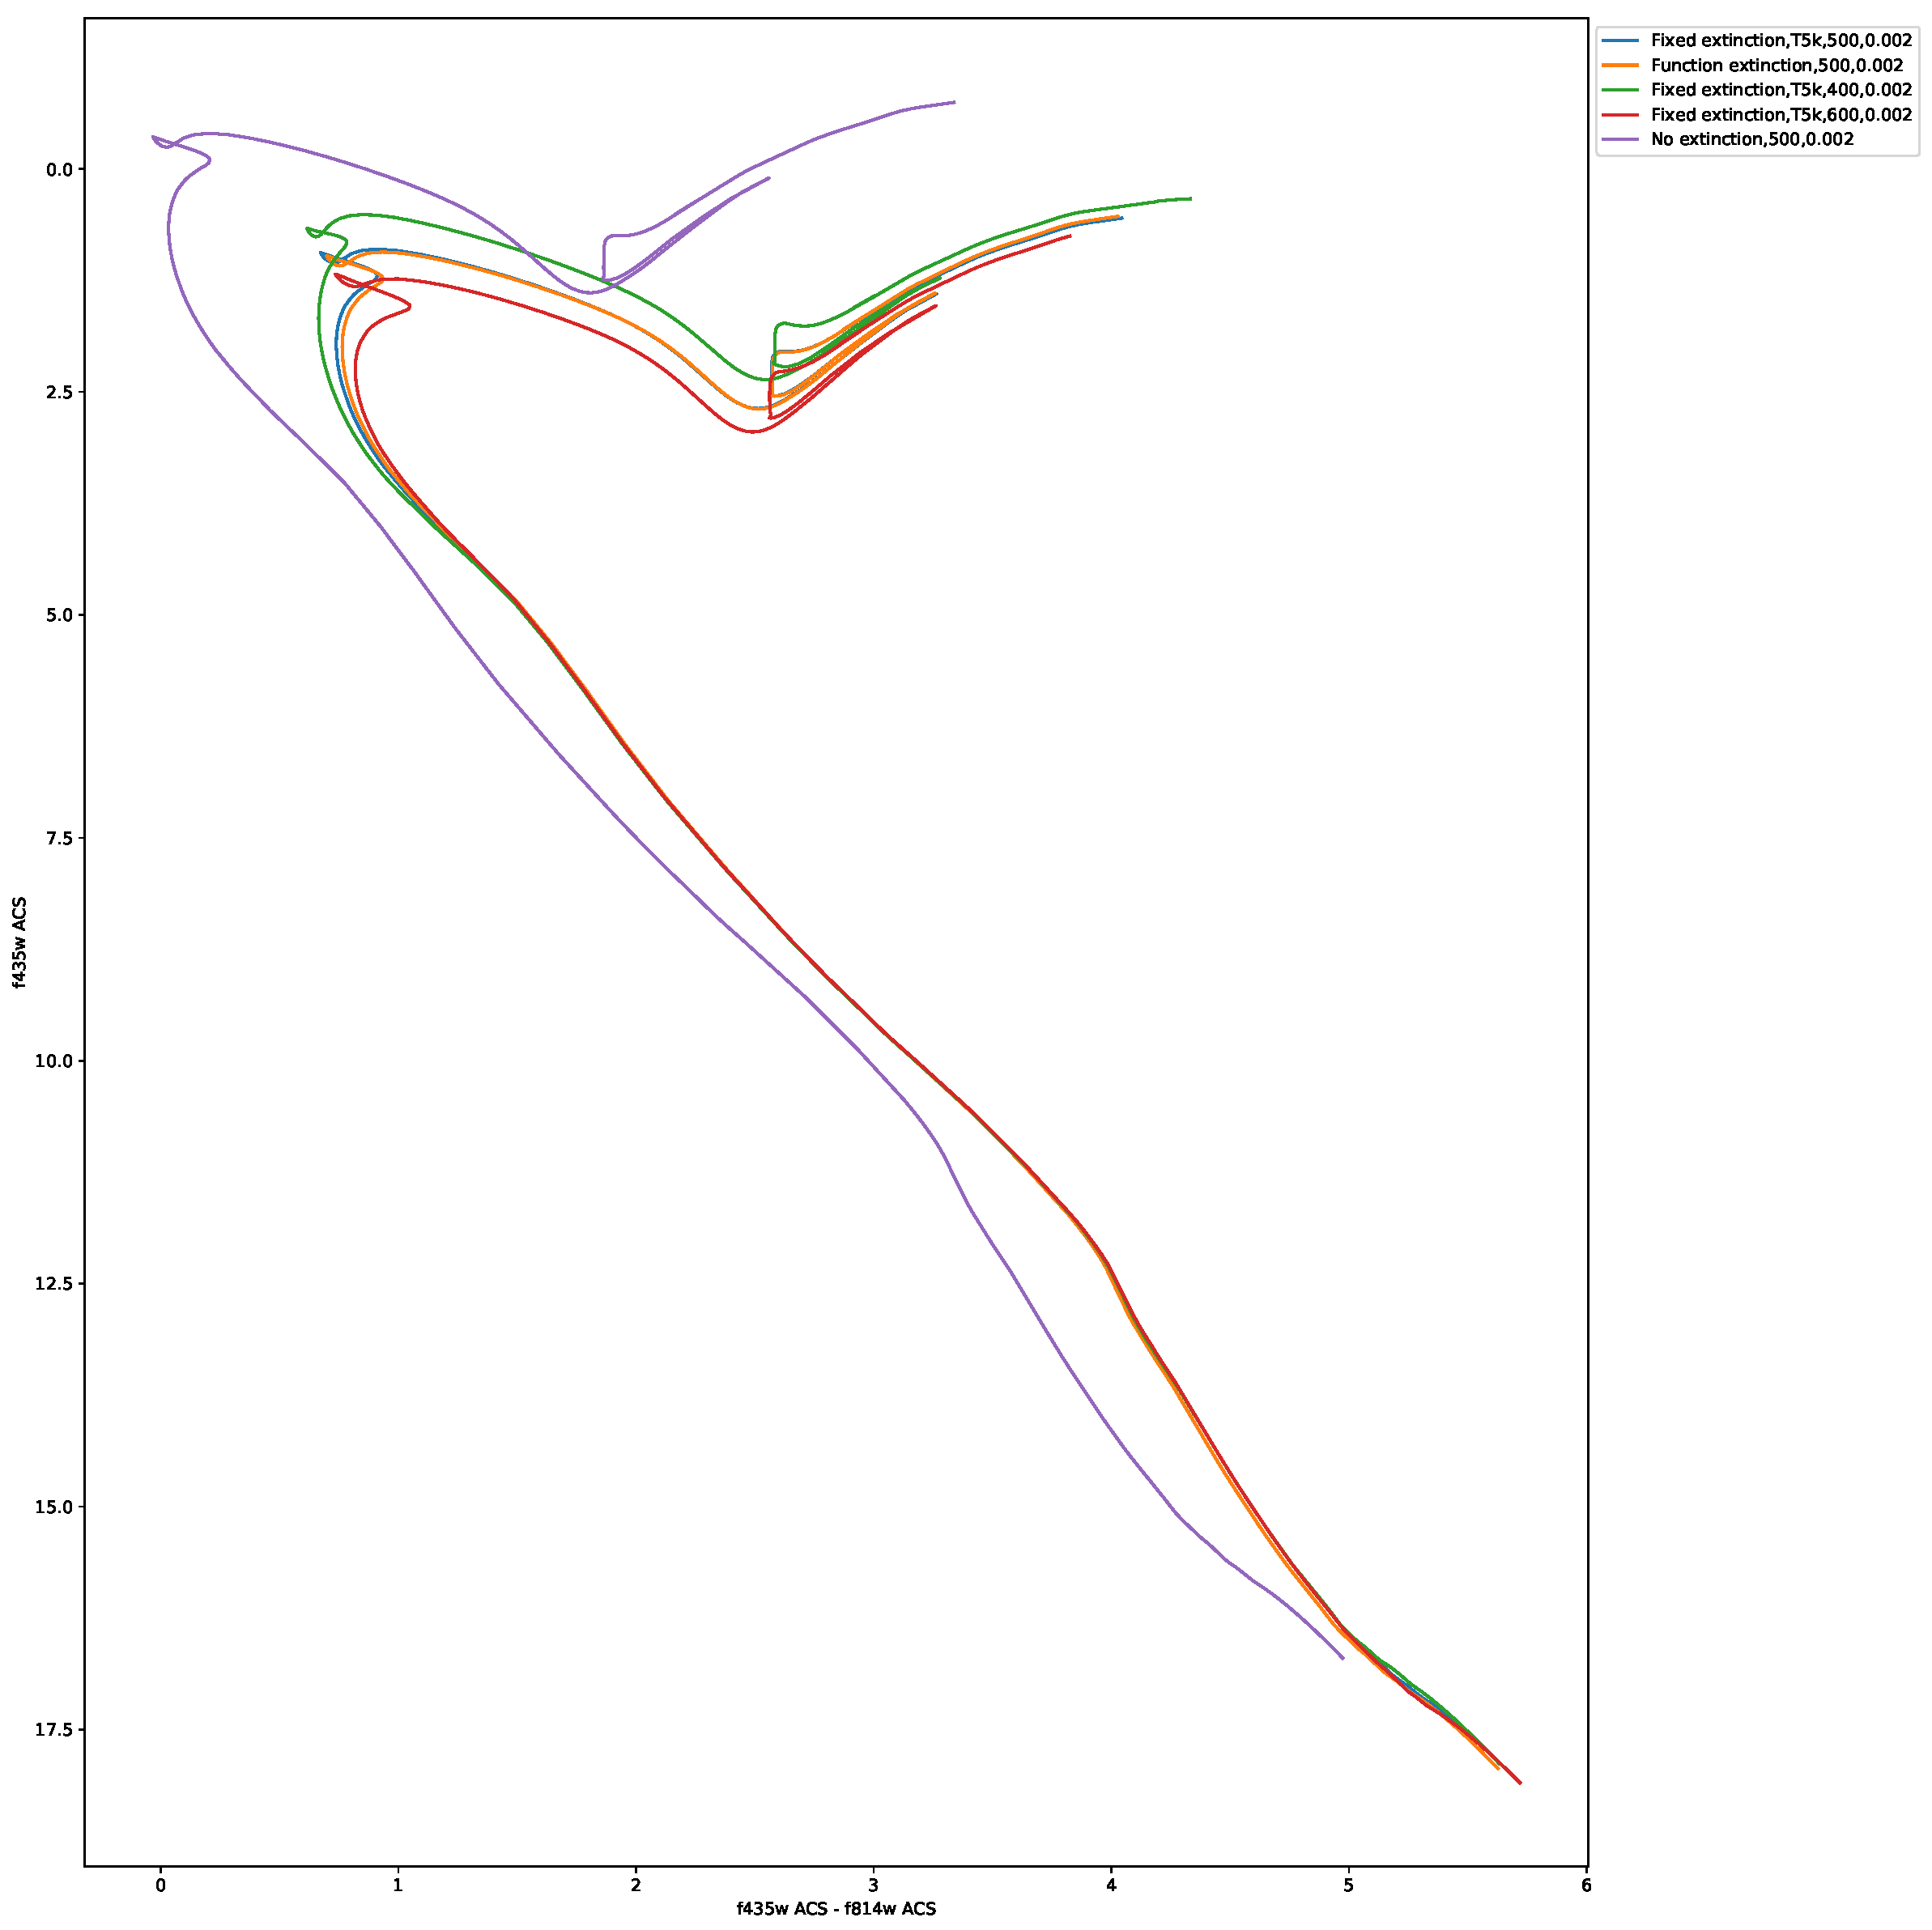
\includegraphics[width=1.0\textwidth]{../basti_isochrones_10_13Gyr/Extinction_T5k_FeH0fix_func_f435wACS_f435wACSmf814wACS_500_400_600_Myr_FeH_0p002_ref_noext_Av_1p0.pdf}
\caption{ACS F435W-(F435W-F814W) CMD with a fixed extinction ratio equal to $(A_{X}/A_{V})_{MS}$ for each filter}
\label{acs_isoc_T5k}
\end{center}
\end{figure}

\begin{figure}[h!]
\begin{center}
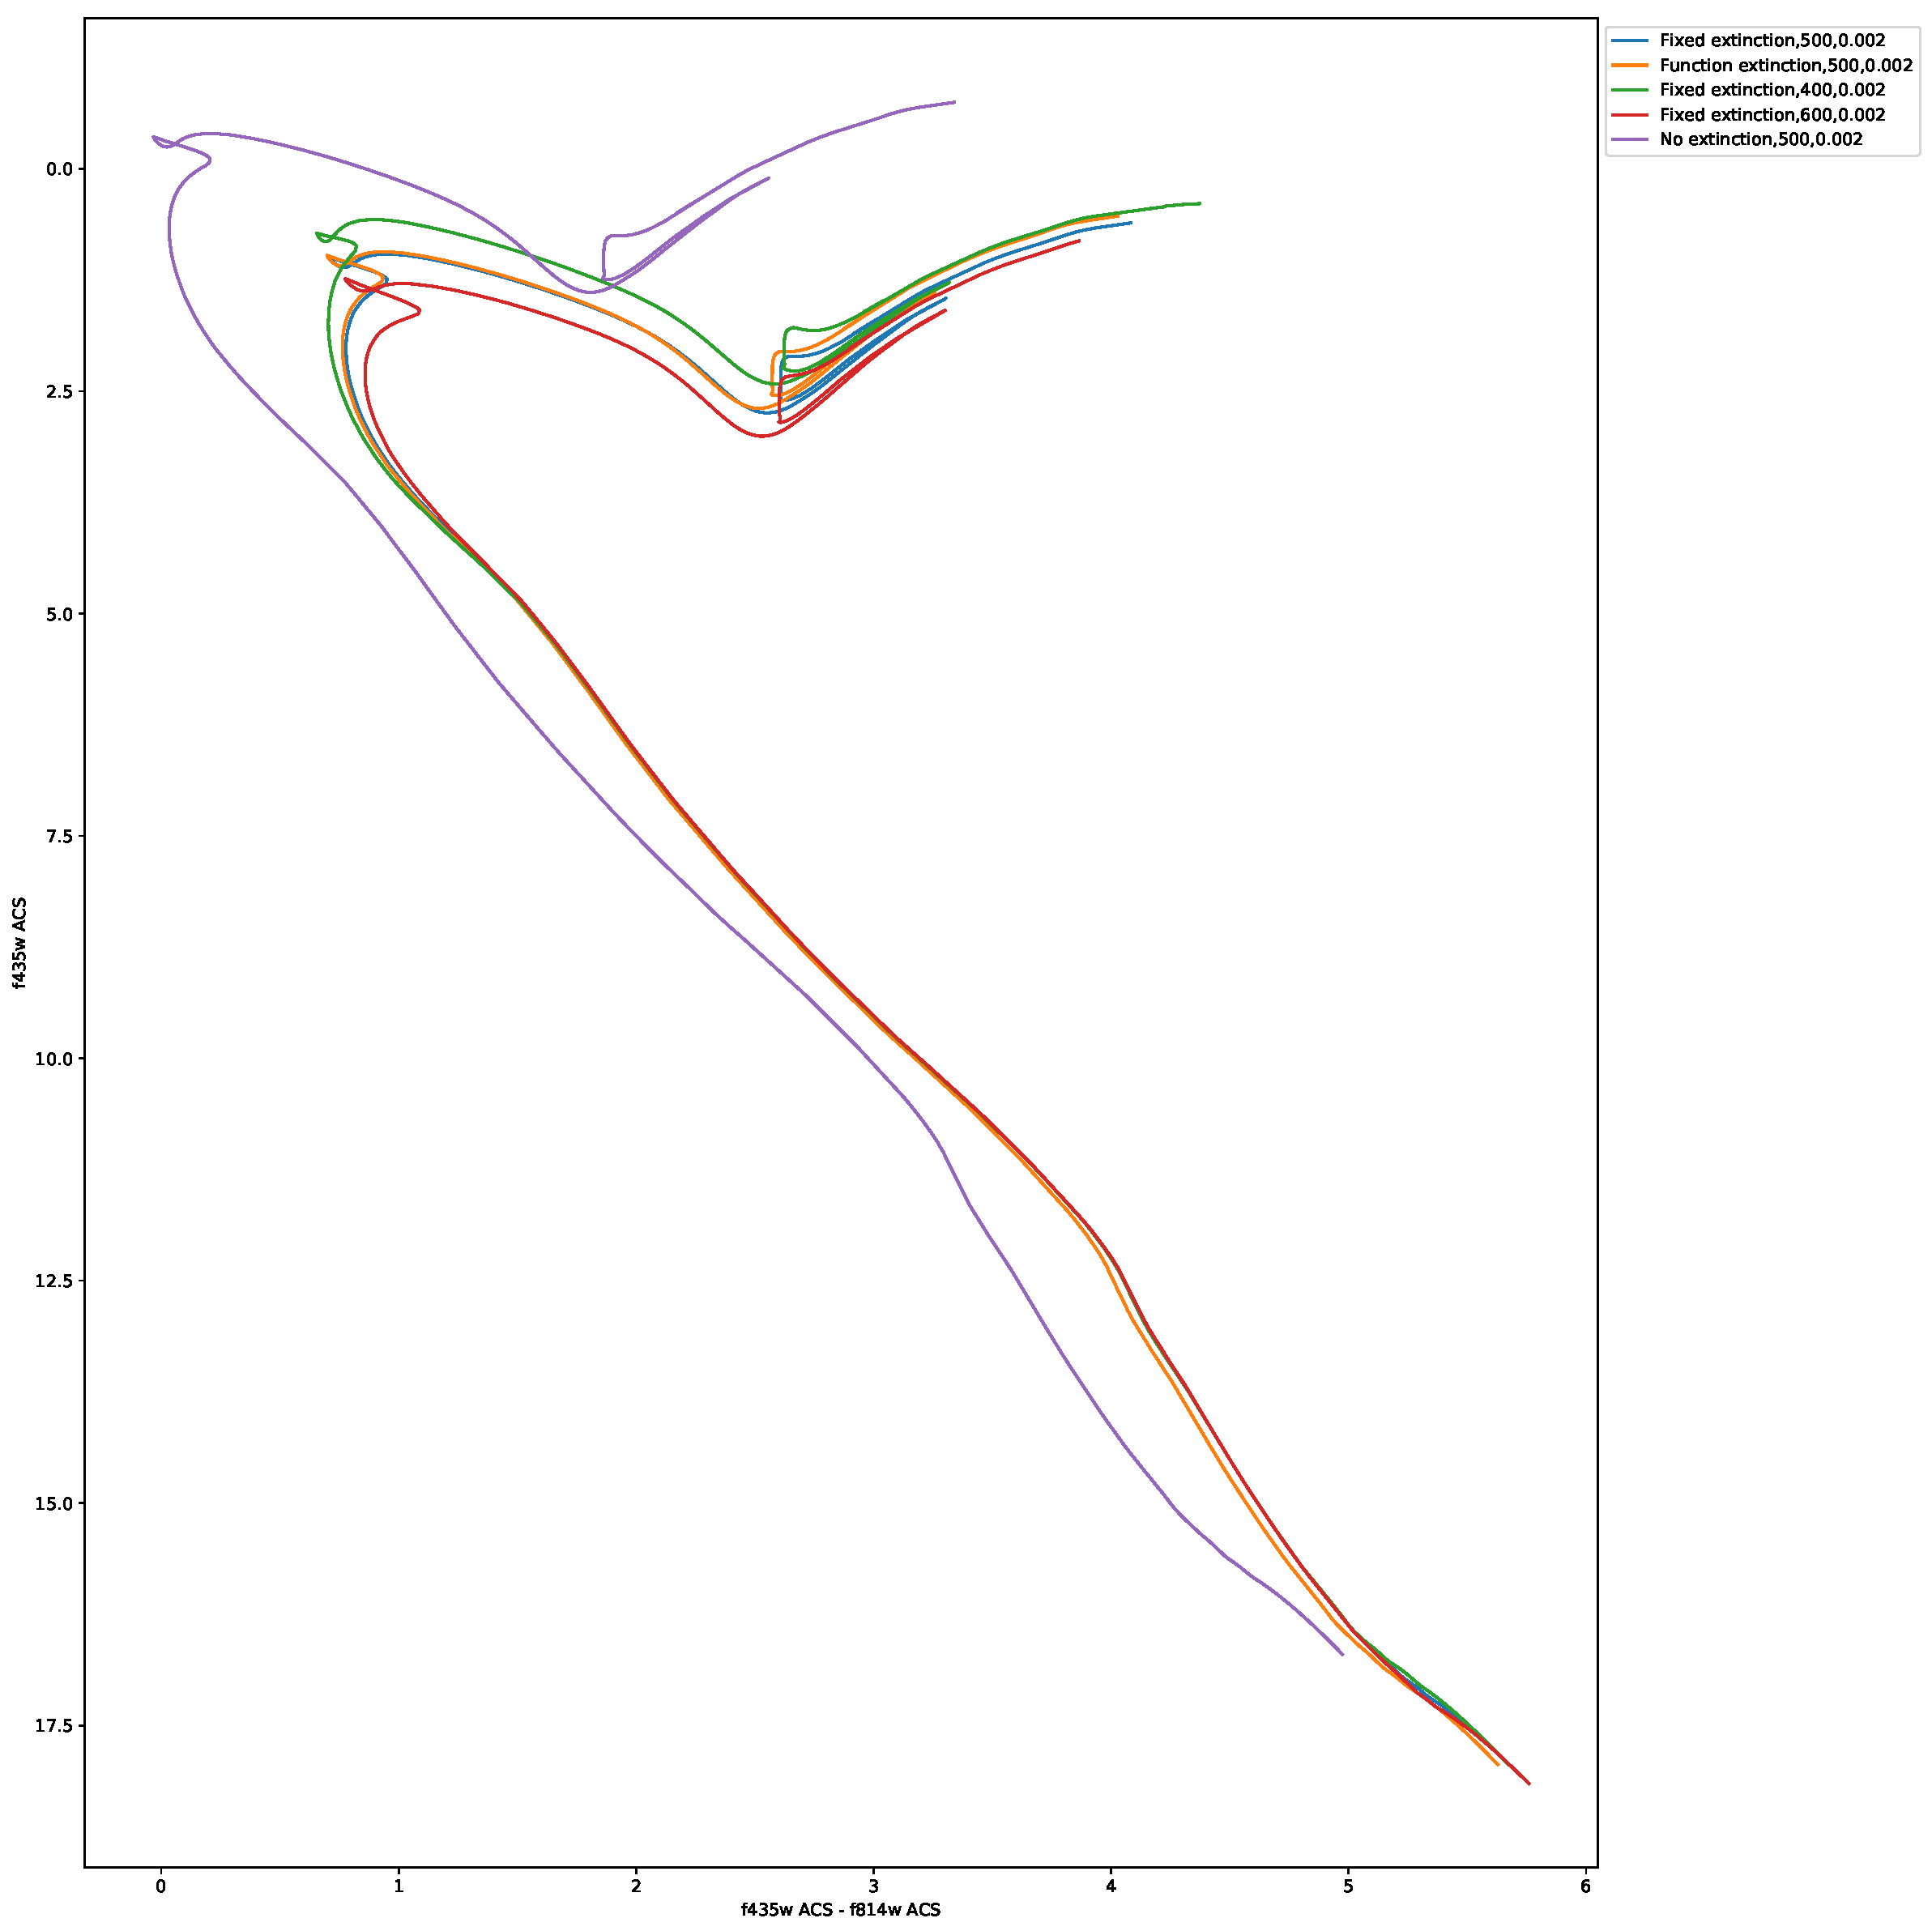
\includegraphics[width=1.0\textwidth]{../basti_isochrones_10_13Gyr/Extinction_T50k_FeH0fix_func_f435wACS_f435wACSmf814wACS_500_400_600_Myr_FeH_0p002_ref_noext_Av_1p0.pdf}
\caption{ACS F435W-(F435W-F814W) CMD with a fixed extinction ratio equal to $(A_{X}/A_{V})_{plat}$ for each filter}
\label{acs_isoc_T50k}
\end{center}
\end{figure}

It can be seen in Figure \ref{acs_isoc_T5k}, by comparing the position of the blue and orange isochrones, that the impact of changing between the FBER and fixed-extinction methods in this CMD is insignificant. Although there are some larger differences in the position of the isochrone in the post-sub-giant branch (SGB) evolutionary stages, this is irrelevant when determining the isochrone age of an observed stellar population.\\*

The result of using $(A_{X}/A_{V})_{plat}$ is not significantly different from that of using $(A_{X}/A_{V})_{MS}$ for this CMD. By comparing Figures \ref{acs_isoc_T5k} and \ref{acs_isoc_T50k}, it is clear that any change in the fixed-extinction $A_{X}/A_{V}$ value used in the F435W and F814W ACS filters (see Figure \ref{just_data_FeH0_ACS}) is insignificant in the context of these isochrones.\\*

\subsection{WFC3} \label{WFC3_isoc}

Two different CMDs were chosen whose filters are part of the WFC3 system. The first is the F555W-(F555W-F814W) CMD. This CMD pairs a wide yellow filter (F555W) with the WFC3's reddest IR wide-field filter. This CMD mimics the pre-existing and widely used Johnson-Cousins $V$-($V-I$) CMD \citep{2014wfc..rept...16S}, which allows direct comparison of observed data with archive data obtained before the creation of the WFC3 filters.\\*

As with the previous ACS CMD, this CMD shows no significant changes in isochrone position resulting from either employing a FBER model or changing the extinction ratio value used for the fixed-value extinction model from $(A_{X}/A_{V})_{plat}$ to $(A_{X}/A_{V})_{MS}$ or vice versa, as demonstrated in Figures \ref{wfc3_isoc1_T5k} and \ref{wfc3_isoc1_T50k}.\\*

\begin{figure}[h!]
\begin{center}
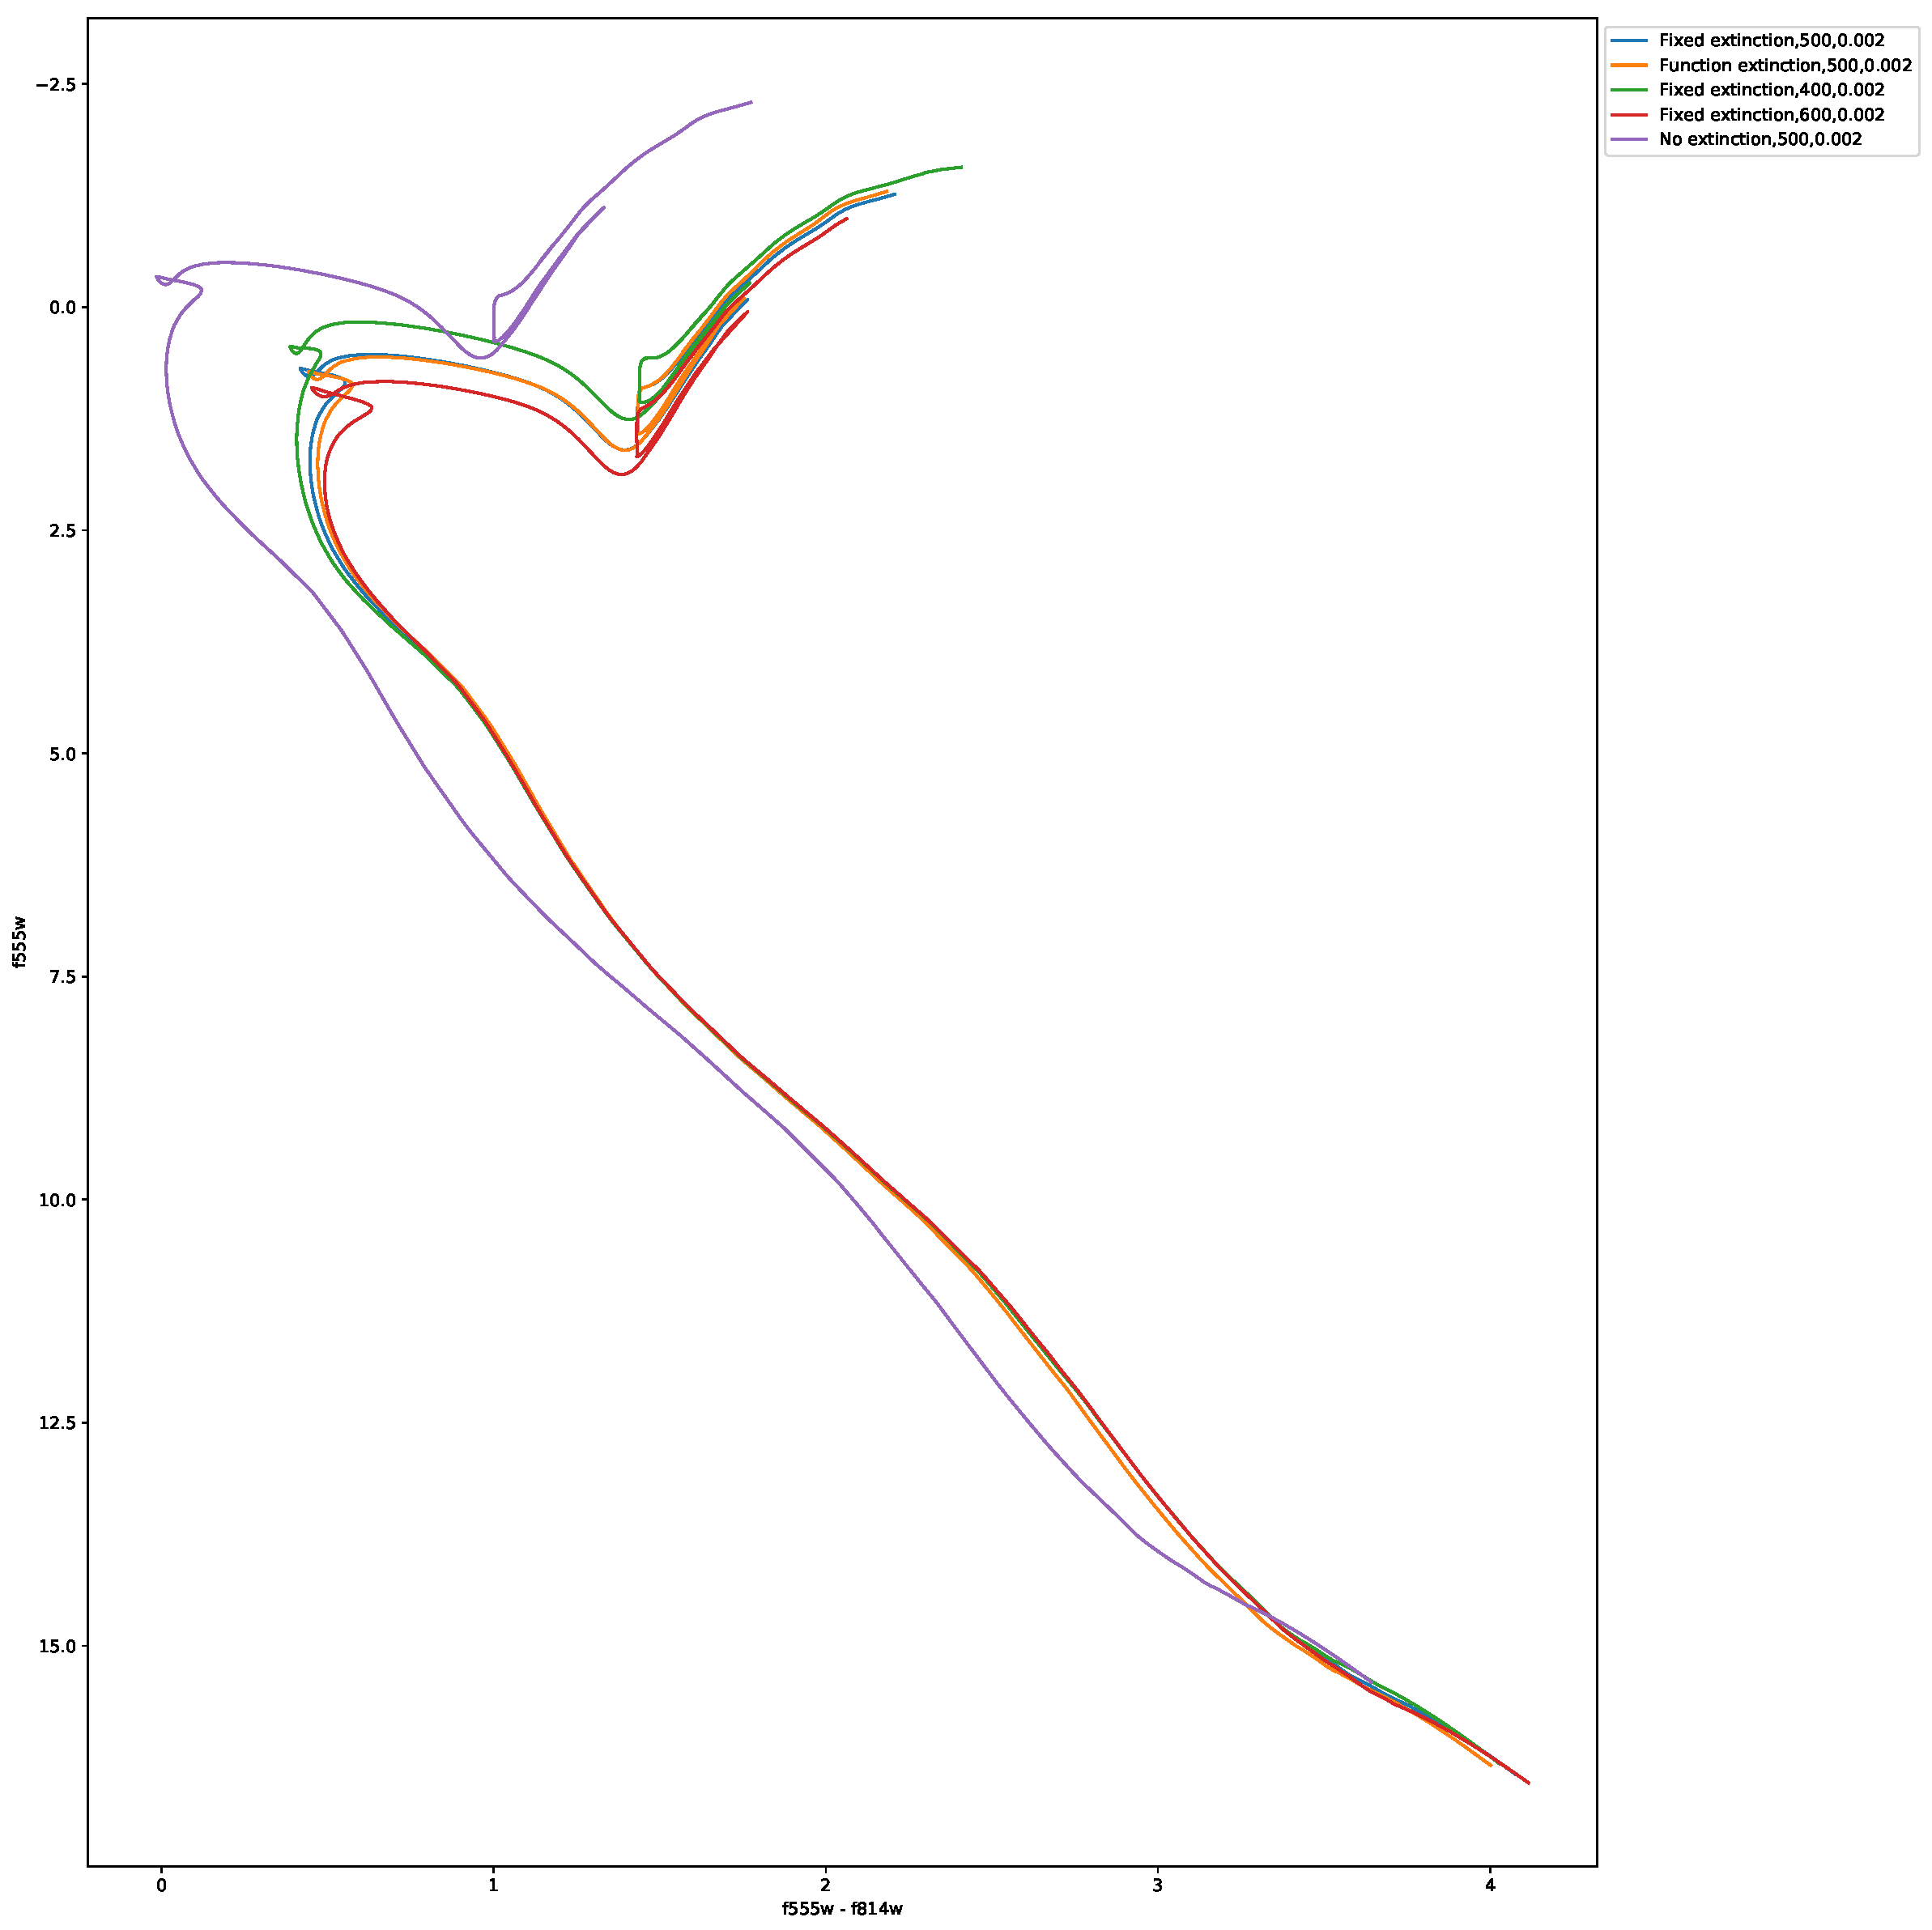
\includegraphics[width=1.0\textwidth]{../basti_isochrones_10_13Gyr/Extinction_T5k_FeH0fix_func_f555w_f555wmf814w_500_400_600_Myr_FeH_0p002_ref_noext_Av_1p0.pdf}
\caption{WFC3 F555W-(F555W-F814W) CMD with a fixed extinction value equal to $(A_{X}/A_{V})_{MS}$ for each filter}
\label{wfc3_isoc1_T5k}
\end{center}
\end{figure}

\begin{figure}[h!]
\begin{center}
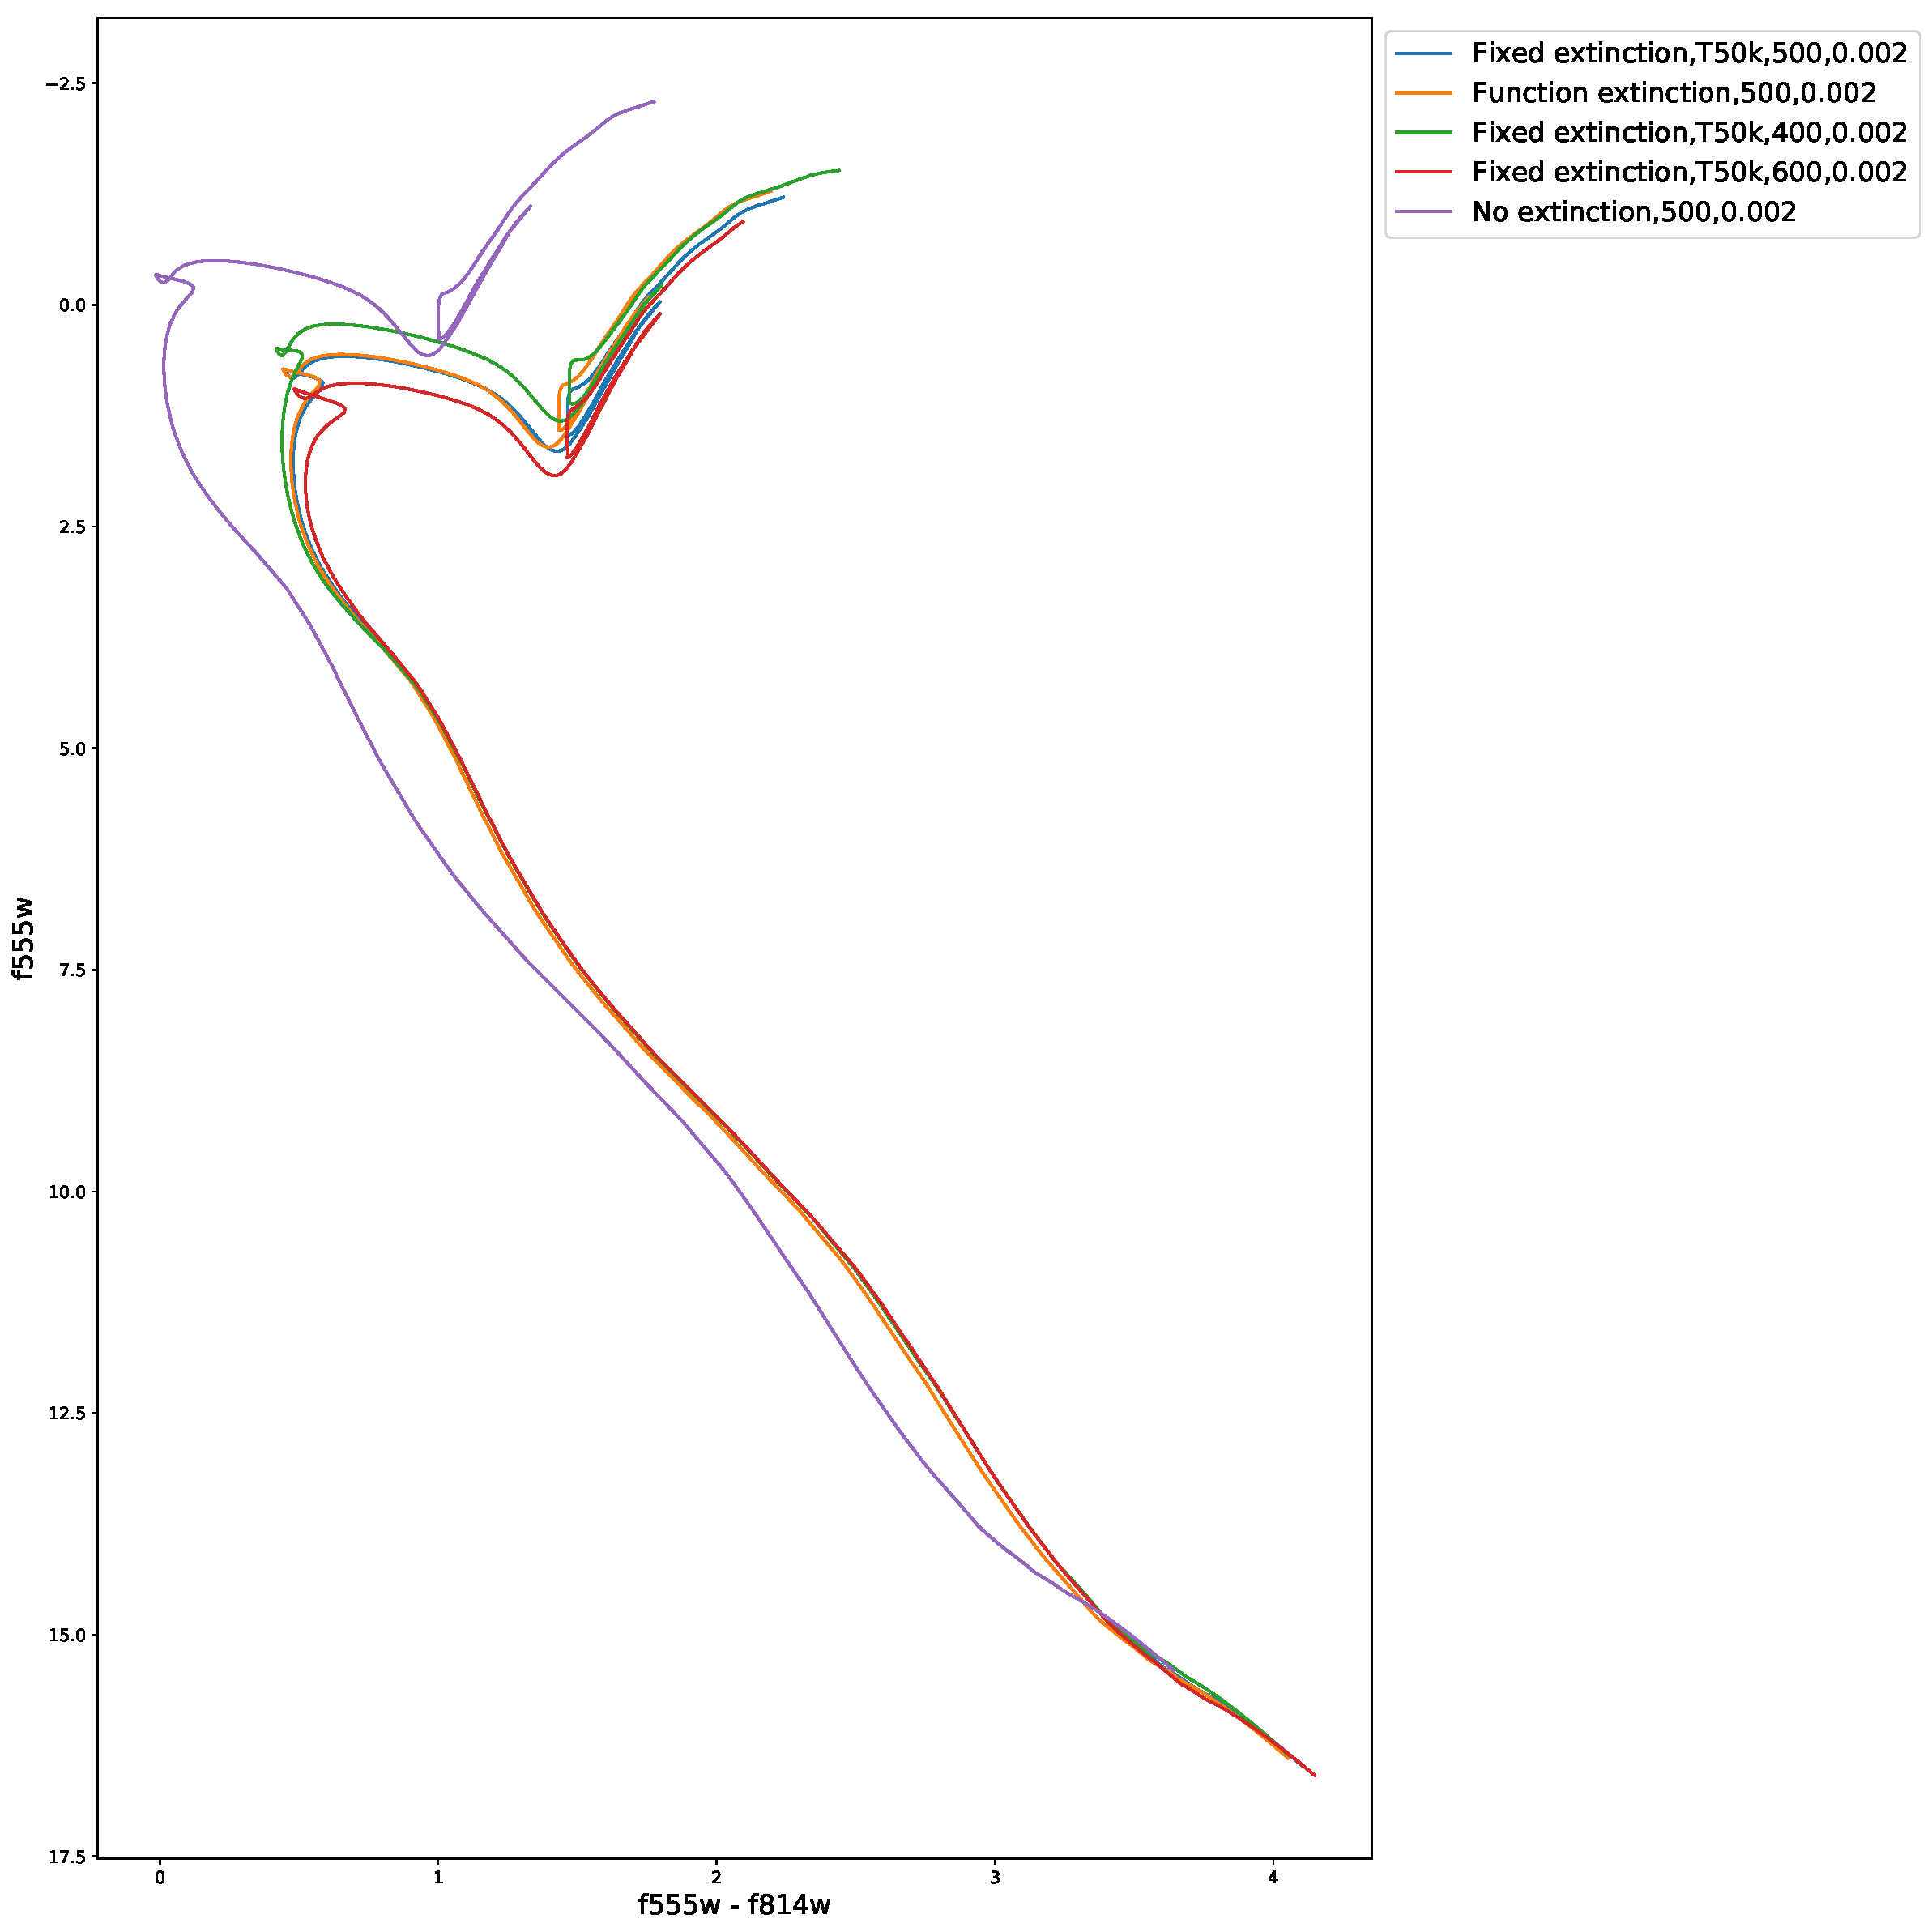
\includegraphics[width=1.0\textwidth]{../basti_isochrones_10_13Gyr/Extinction_T50k_FeH0fix_func_f555w_f555wmf814w_500_400_600_Myr_FeH_0p002_ref_noext_Av_1p0.pdf}
\caption{WFC3 F555W-(F555W-F814W) CMD with a fixed extinction value equal to $(A_{X}/A_{V})_{plat}$ for each filter}
\label{wfc3_isoc1_T50k}
\end{center}
\end{figure}

The second WFC3 CMD that was studied is the F814W-(F275W-F814W) CMD. The filters that form this CMD cover the soft-UV and near-IR spectral regions. The high baseline wavelength coverage of this combination of filters makes the colour index more sensitive to differences in $T_{\textnormal{eff}}$ in hot horizontal branch (HB) stars. These objects are important due to direct helium abundance measurements (from absorption lines) being available in globular clusters only for HB stars with 8000 $\lesssim T_{\textnormal{eff}}$ / K $\lesssim$ 11500 \citep{2018MNRAS.475.4088L}. \\*

\begin{figure}[h!]
\begin{center}
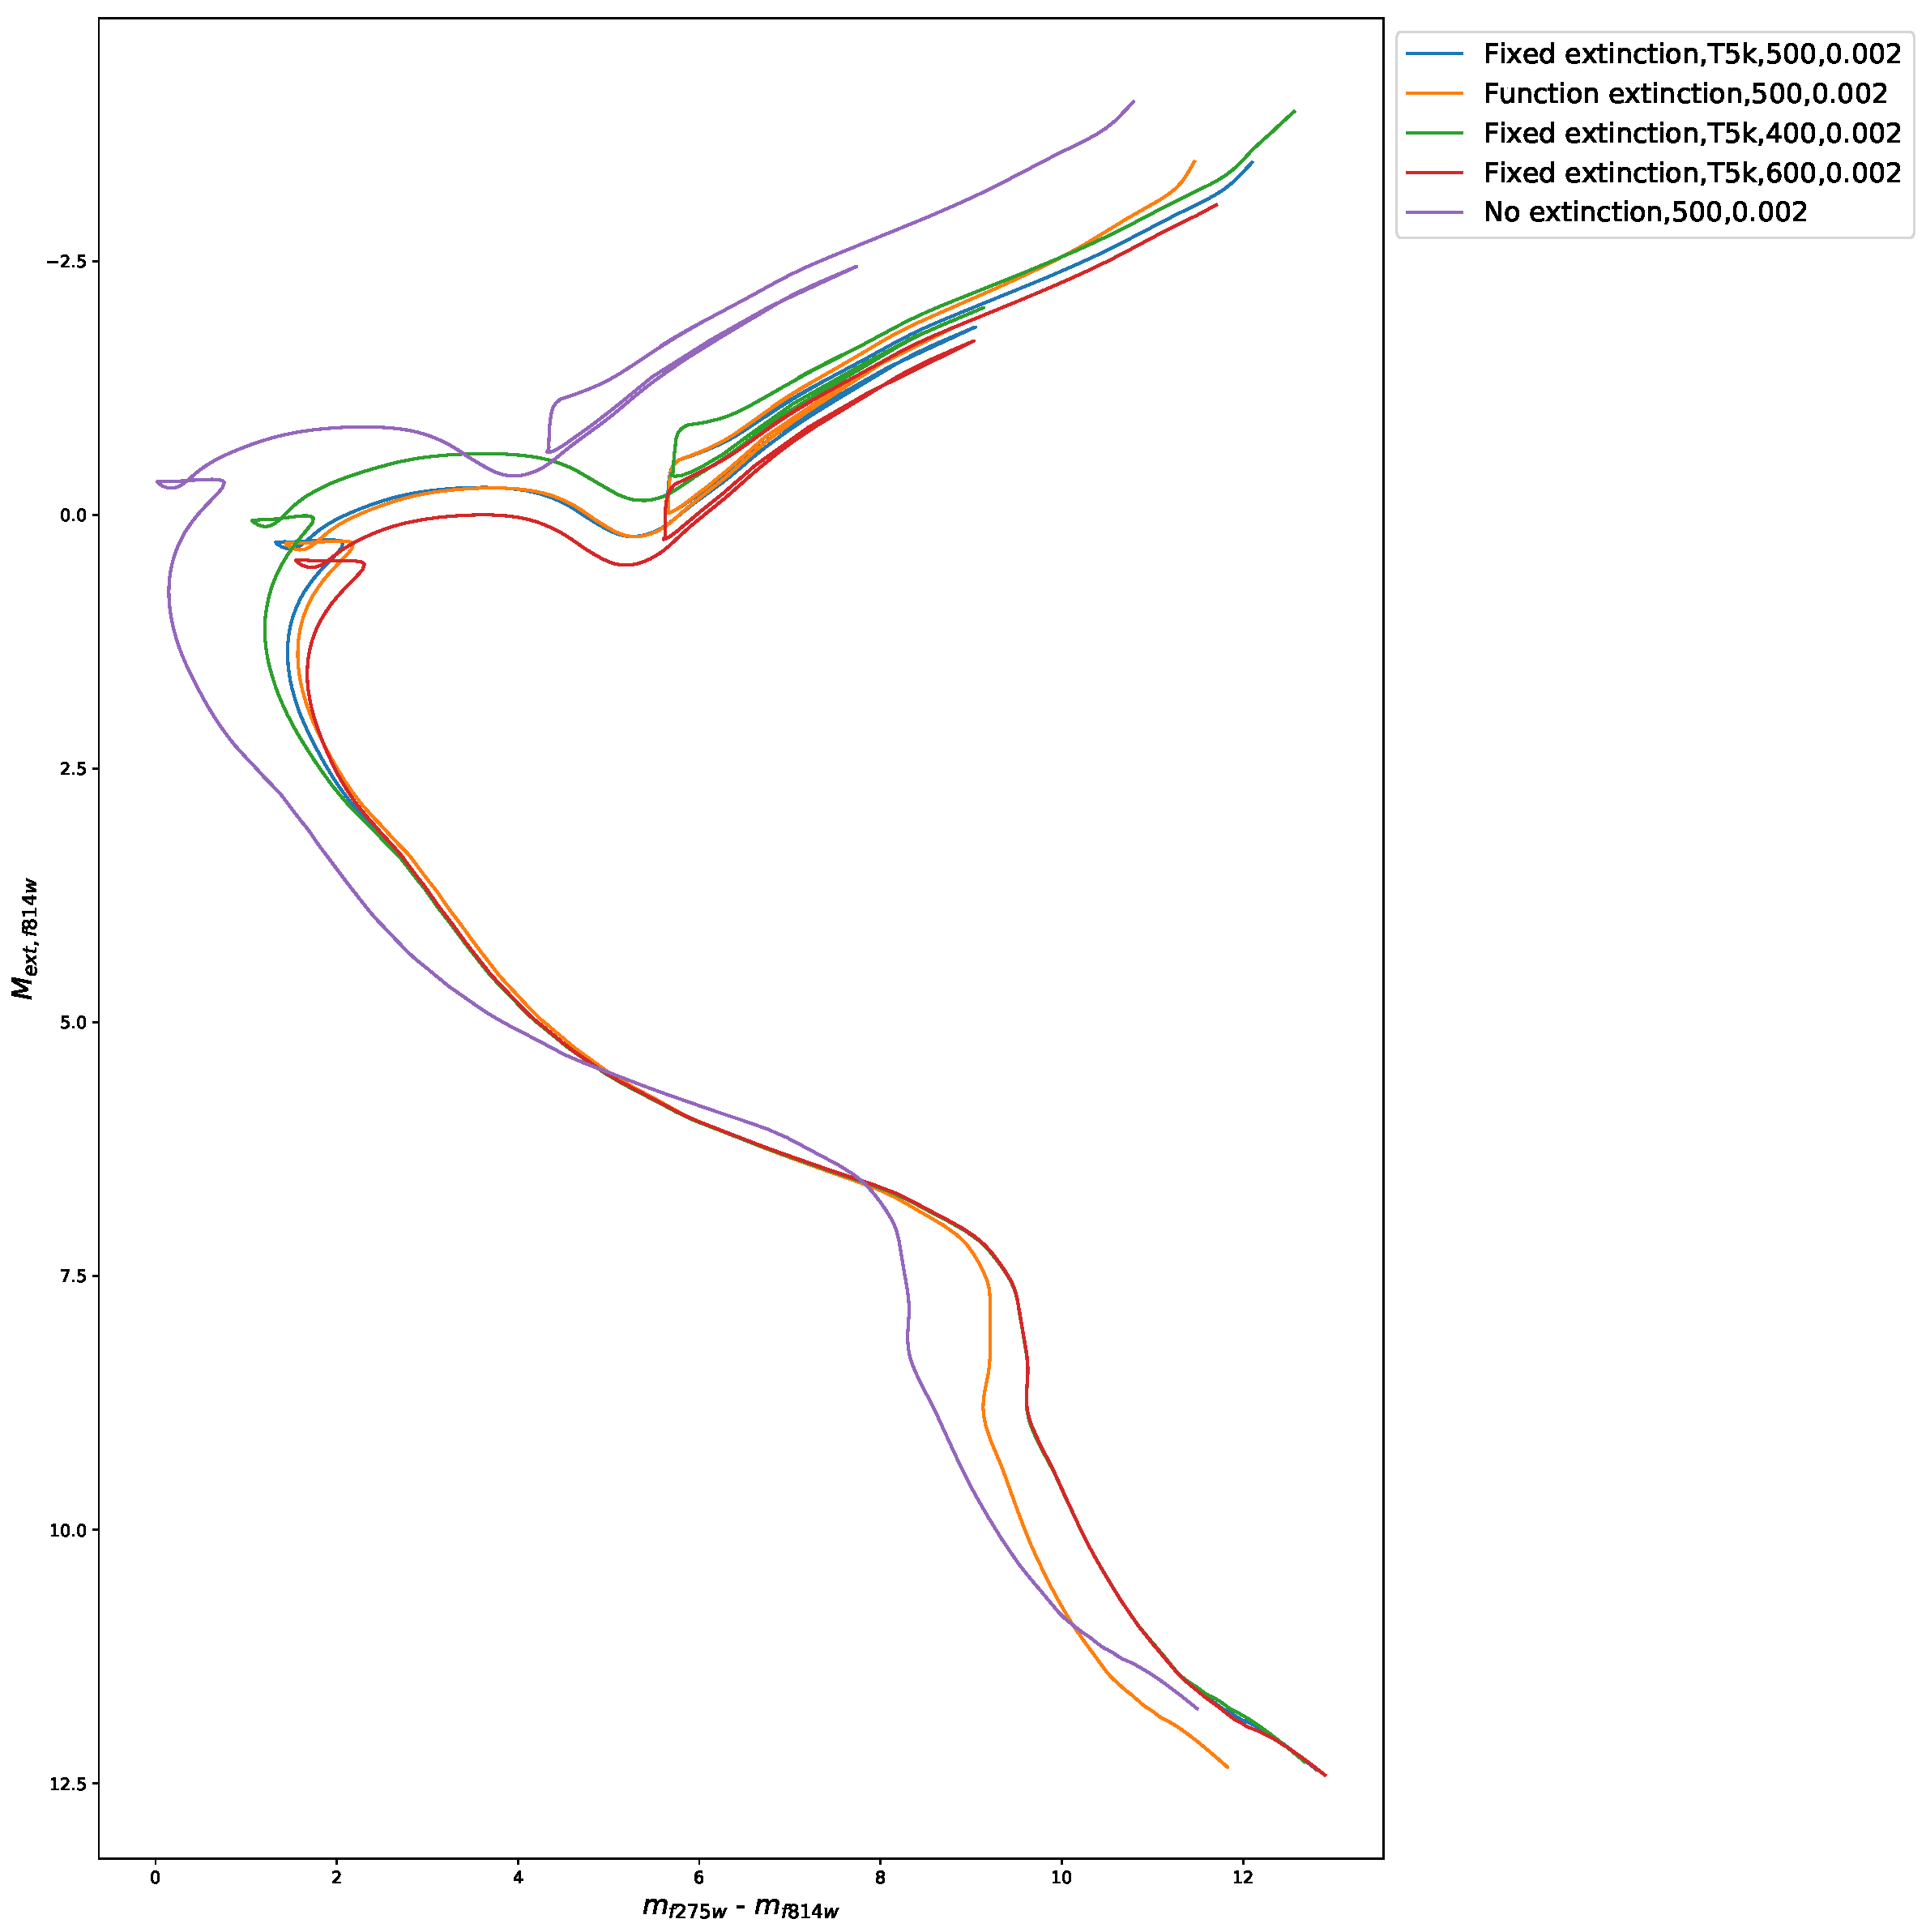
\includegraphics[width=1.0\textwidth]{../basti_isochrones_10_13Gyr/Extinction_T5k_FeH0fix_func_f814w_f275wmf814w_500_400_600_Myr_FeH_0p002_ref_noext_Av_1p0.pdf}
\caption{WFC3 F814W-(F275W-F814W) CMD with a fixed extinction value equal to $(A_{X}/A_{V})_{MS}$ for each filter.}
\label{wfc3_isoc2_T5k}
\end{center}
\end{figure}

\begin{figure}[h!]
\begin{center}
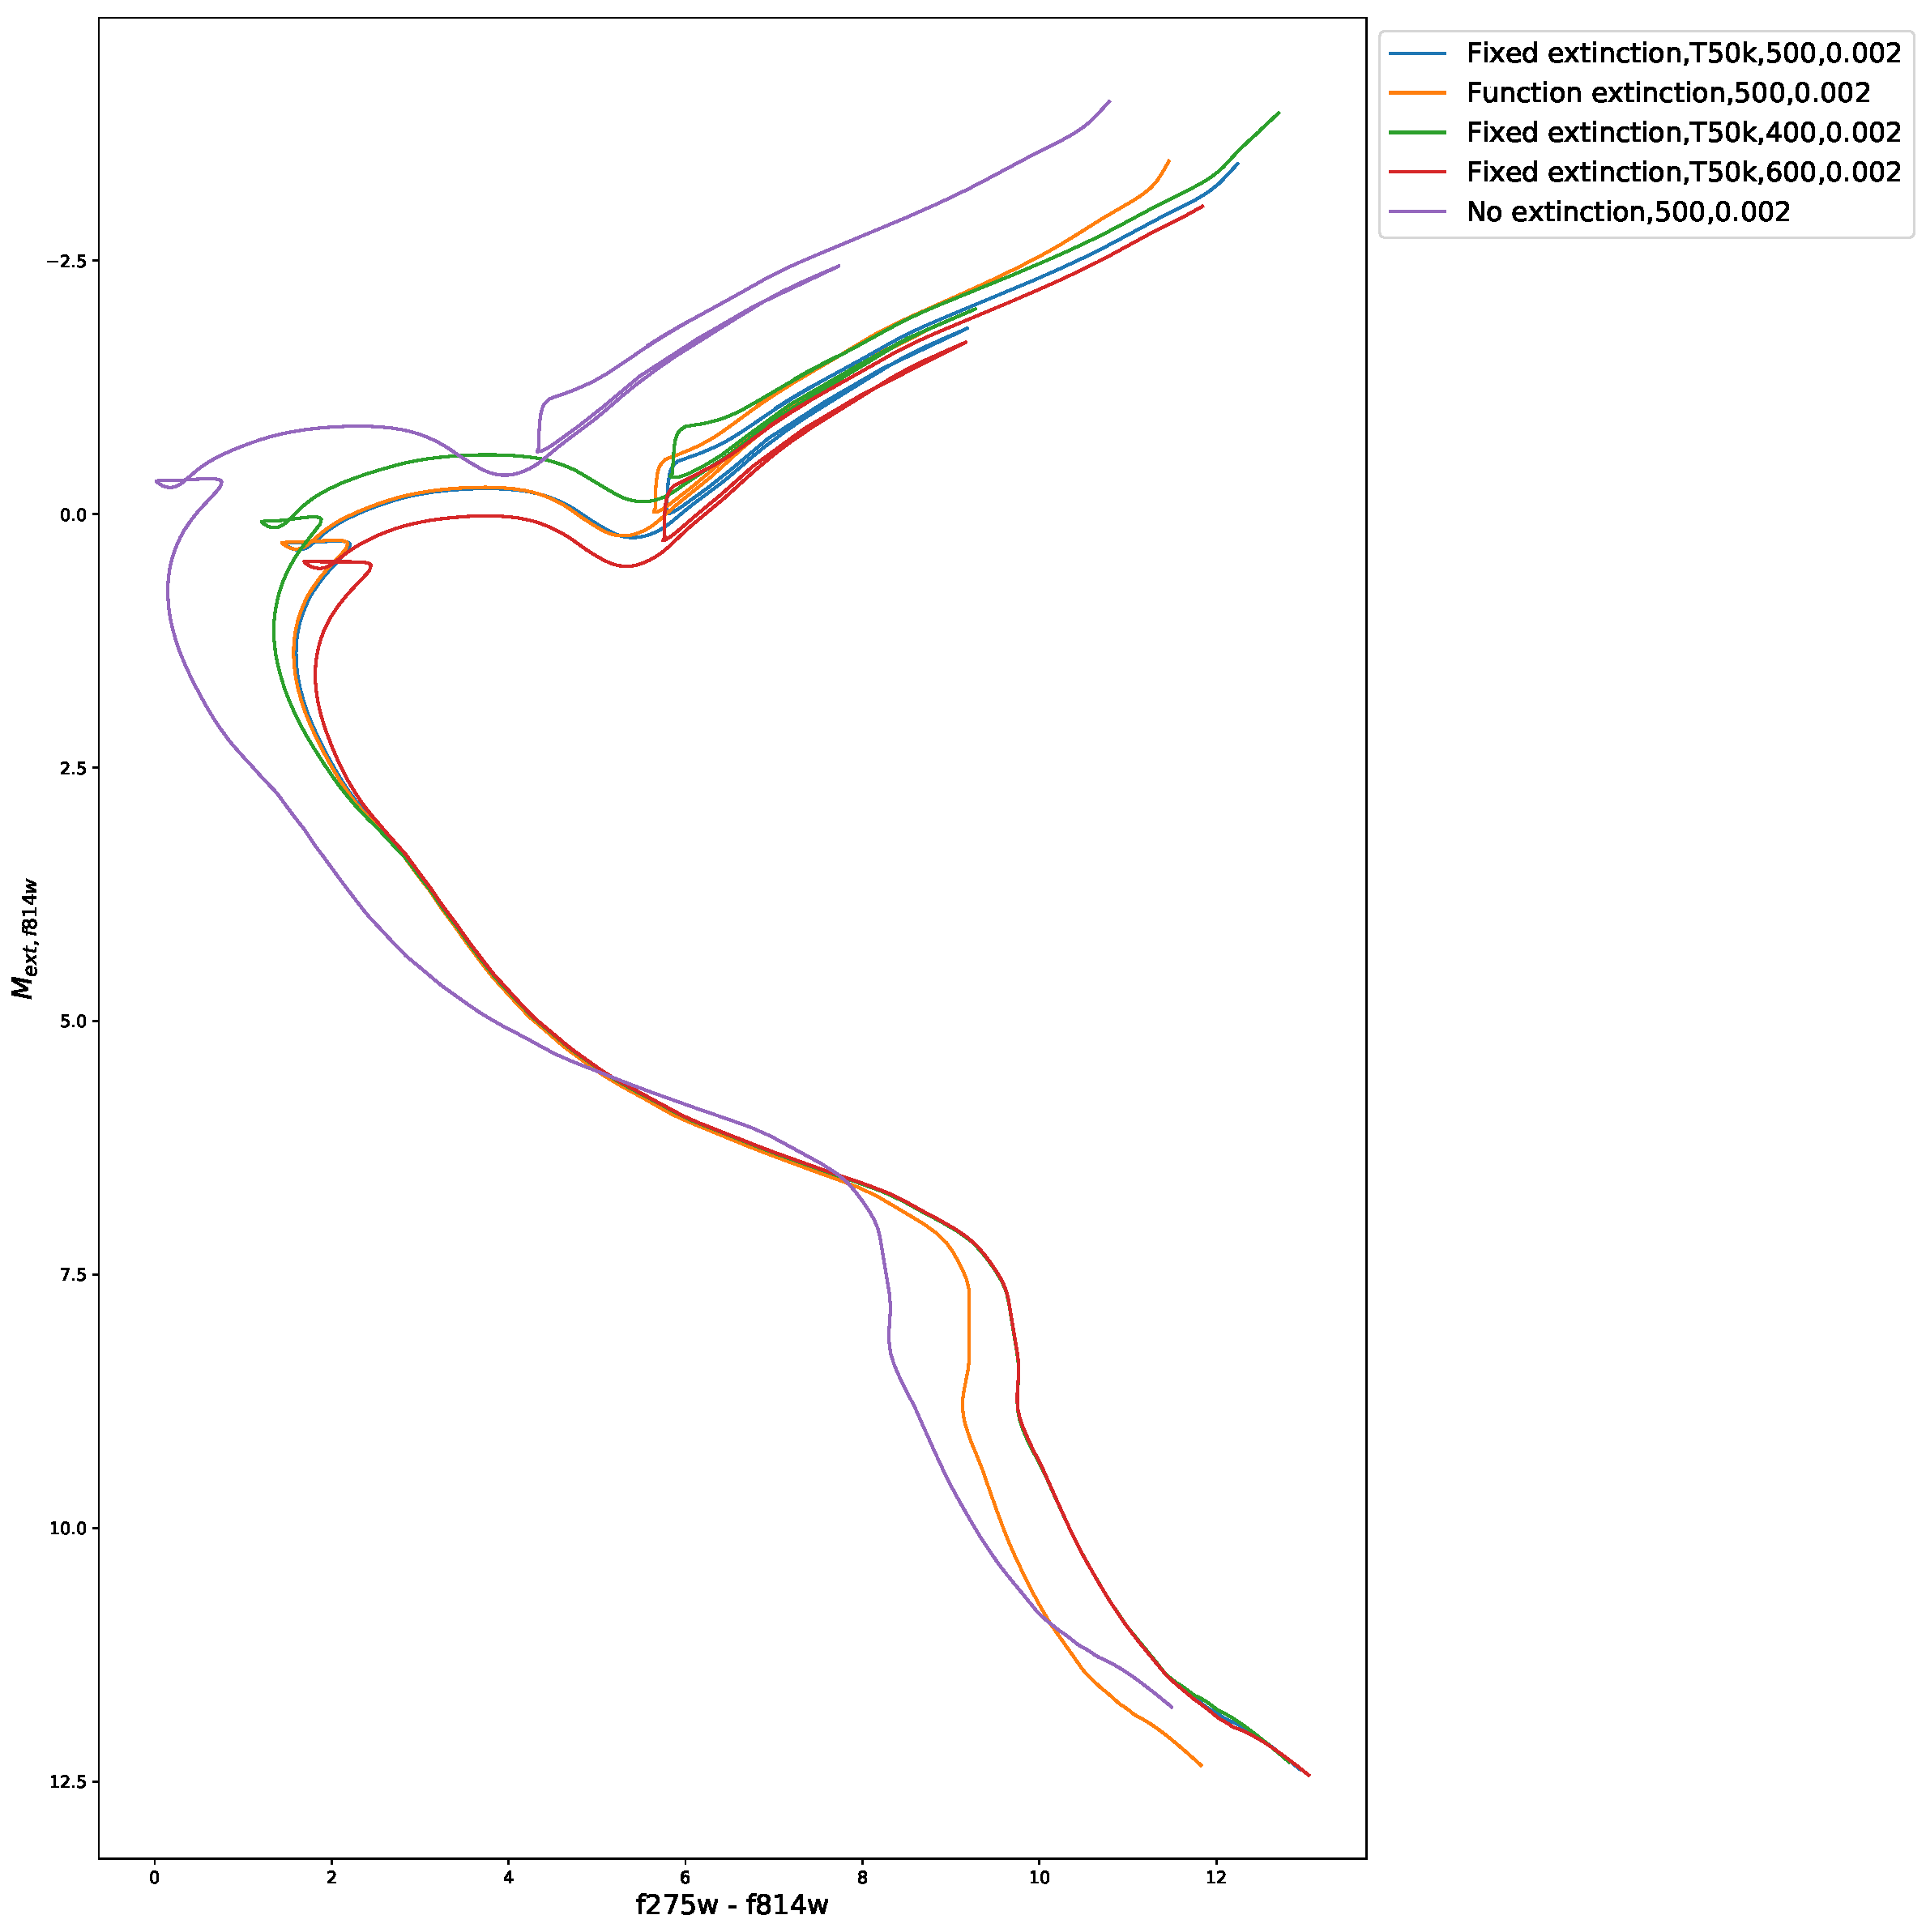
\includegraphics[width=1.0\textwidth]{../basti_isochrones_10_13Gyr/Extinction_T50k_FeH0fix_func_f814w_f275wmf814w_500_400_600_Myr_FeH_0p002_ref_noext_Av_1p0.pdf}
\caption{WFC3 F814W-(F275W-F814W) CMD with a fixed extinction value equal to $(A_{X}/A_{V})_{plat}$ for each filter}
\label{wfc3_isoc2_T50k}
\end{center}
\end{figure}

In Figure \ref{wfc3_isoc2_T5k}, it can be seen that, when the $(A_{X}/A_{V})_{MS}$ fixed model is being used as a reference (i.e., the models' upper main sequences below the MSTO are aligned), the position of the MSTO of the FBER 500 Myr isochrone aligns with that of the 600 Myr fixed-ratio isochrone. By the point at which the MS hook \citep{1998MNRAS.298..525P} appears, the FBER isochrone has almost realigned with the 500 Myr fixed-ratio isochrone. There are significant differences between the two 500 Myr isochrones after the lower portion of the RGB. In the lower main sequence, all isochrones with fixed extinction ratios appear significantly redder, while the infrared F814W magnitudes appear to be more or less unchanged from the FBER case. This can only be the result of significant differences in $A_{F275W}/A_{V}$ values between stars in the upper main sequence (higher $T_{\textnormal{eff}}$ values) and in the lower main sequence (lower $T_{\textnormal{eff}}$ values), as these differences are not reflected in the fixed-extinction models. \\*

As shown in Figure \ref{wfc3_isoc2_T50k}, choosing $(A_{X}/A_{V})_{plat}$ for the fixed-extinction isochrones leads to those isochrones shifting down and to the right in the CMD. Ironically, the higher $T_{\textnormal{eff}}$ value of 50,000 K used, which is far greater than any $T_{\textnormal{eff}}$ values present in the isochrone data, brings the MSTO positions of the two 500 Myr isochrones back into alignment. However, the use of $(A_{X}/A_{V})_{plat}$ increases the lower main sequence gap between the fixed-extinction and FBER isochrones. Beyond the lower main sequence, the misalignment between the two 500 Myr isochrones now begins at a later stage in the evolutionary cycle, at the base of the RGB. \\*

Furthermore, there is a possibility of the extinction-related lower main sequence discrepancy causing a discrepancy between the estimated metallicities in the FBER and fixed-extinction isochrones when they are fitted to the observed CMD of a cluster, as the CMD position of this part of the isochrone is the most sensitive to changes in isochrone metallicity.\\*

\subsection{Gaia} \label{Gaia_isoc}

The photometric filters in Gaia, as shown by their respective response functions in Figure \ref{Gaia_response_funcs}, are designed such that the only useful colour index is the ($G_{\textnormal{bp}}-G_{\textnormal{rp}}$) index, with the widest filter ($G$) being on the vertical axis.\\*

\begin{figure}[h!]
\begin{center}
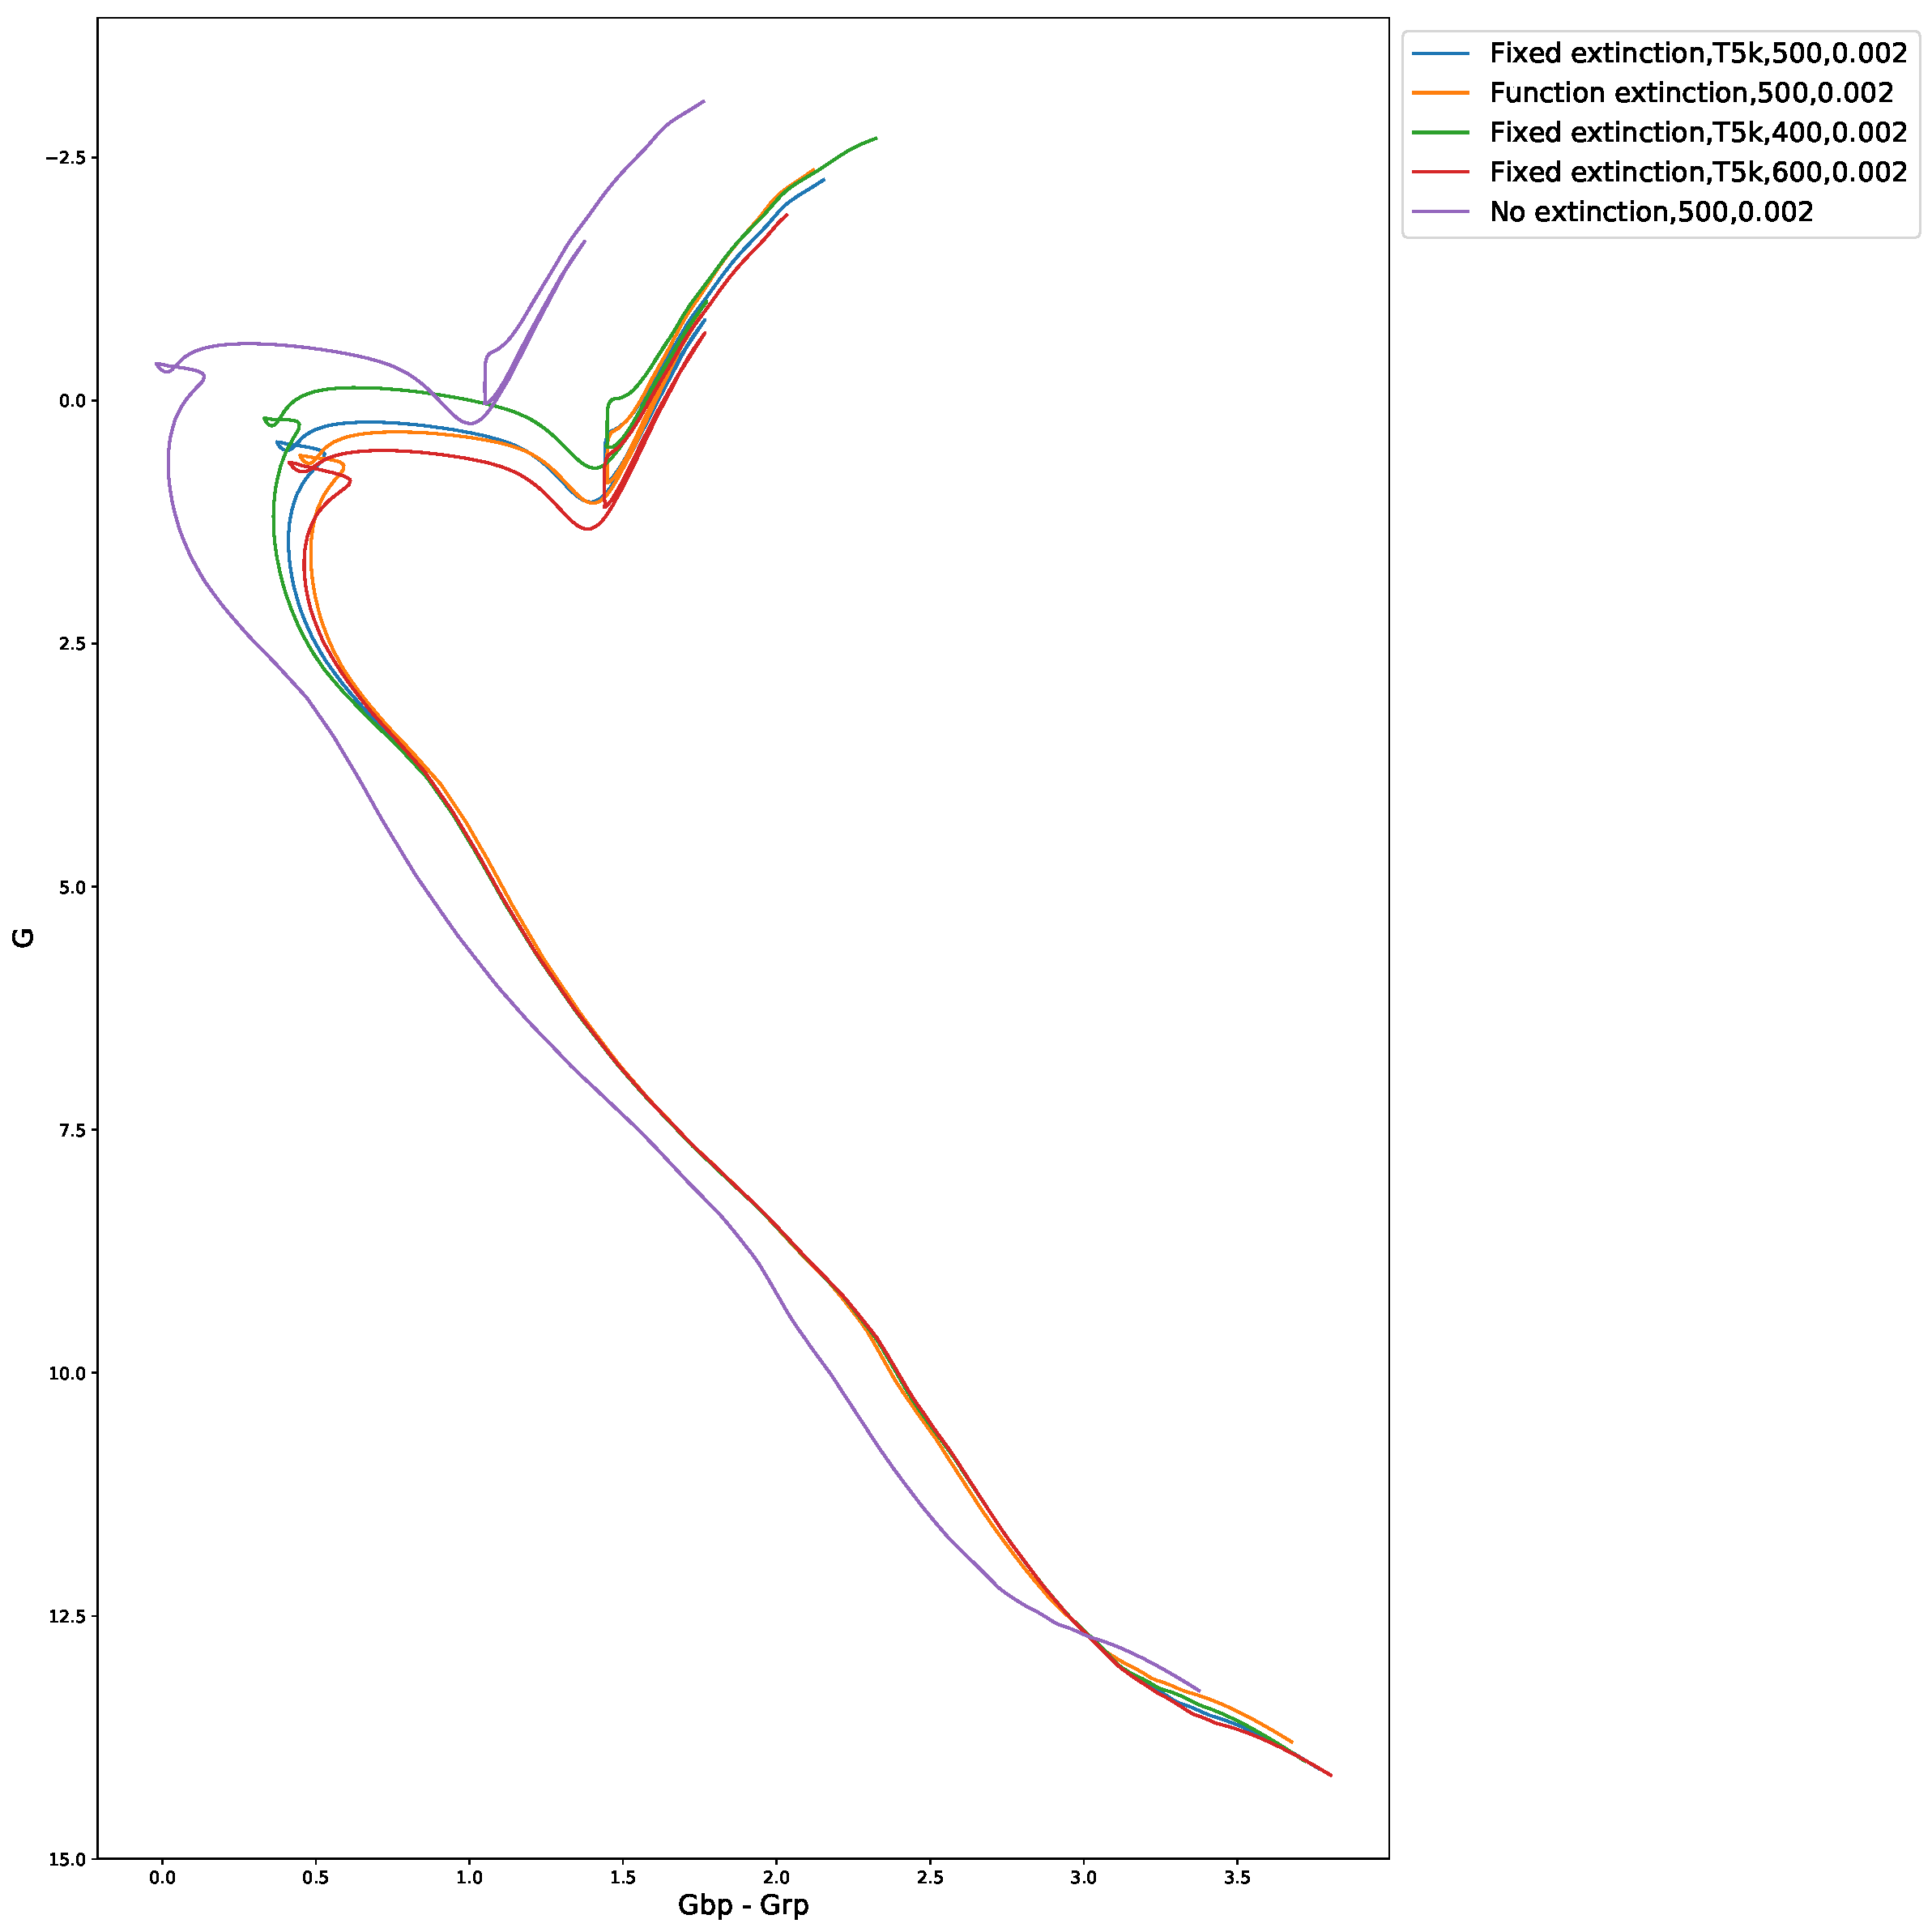
\includegraphics[width=1.0\textwidth]{../basti_isochrones_10_13Gyr/Extinction_T5k_FeH0fix_func_G_GbpmGrp_500_400_600_Myr_FeH_0p002_ref_noext_Av_1p0.pdf}
\caption{Gaia $G$-($G_{\textnormal{bp}}$-$G_{\textnormal{rp}}$) CMD with a fixed extinction value equal to $(A_{X}/A_{V})_{MS}$ for each filter}
\label{gaia_isoc_T5k}
\end{center}
\end{figure}

\begin{figure}[h!]
\begin{center}
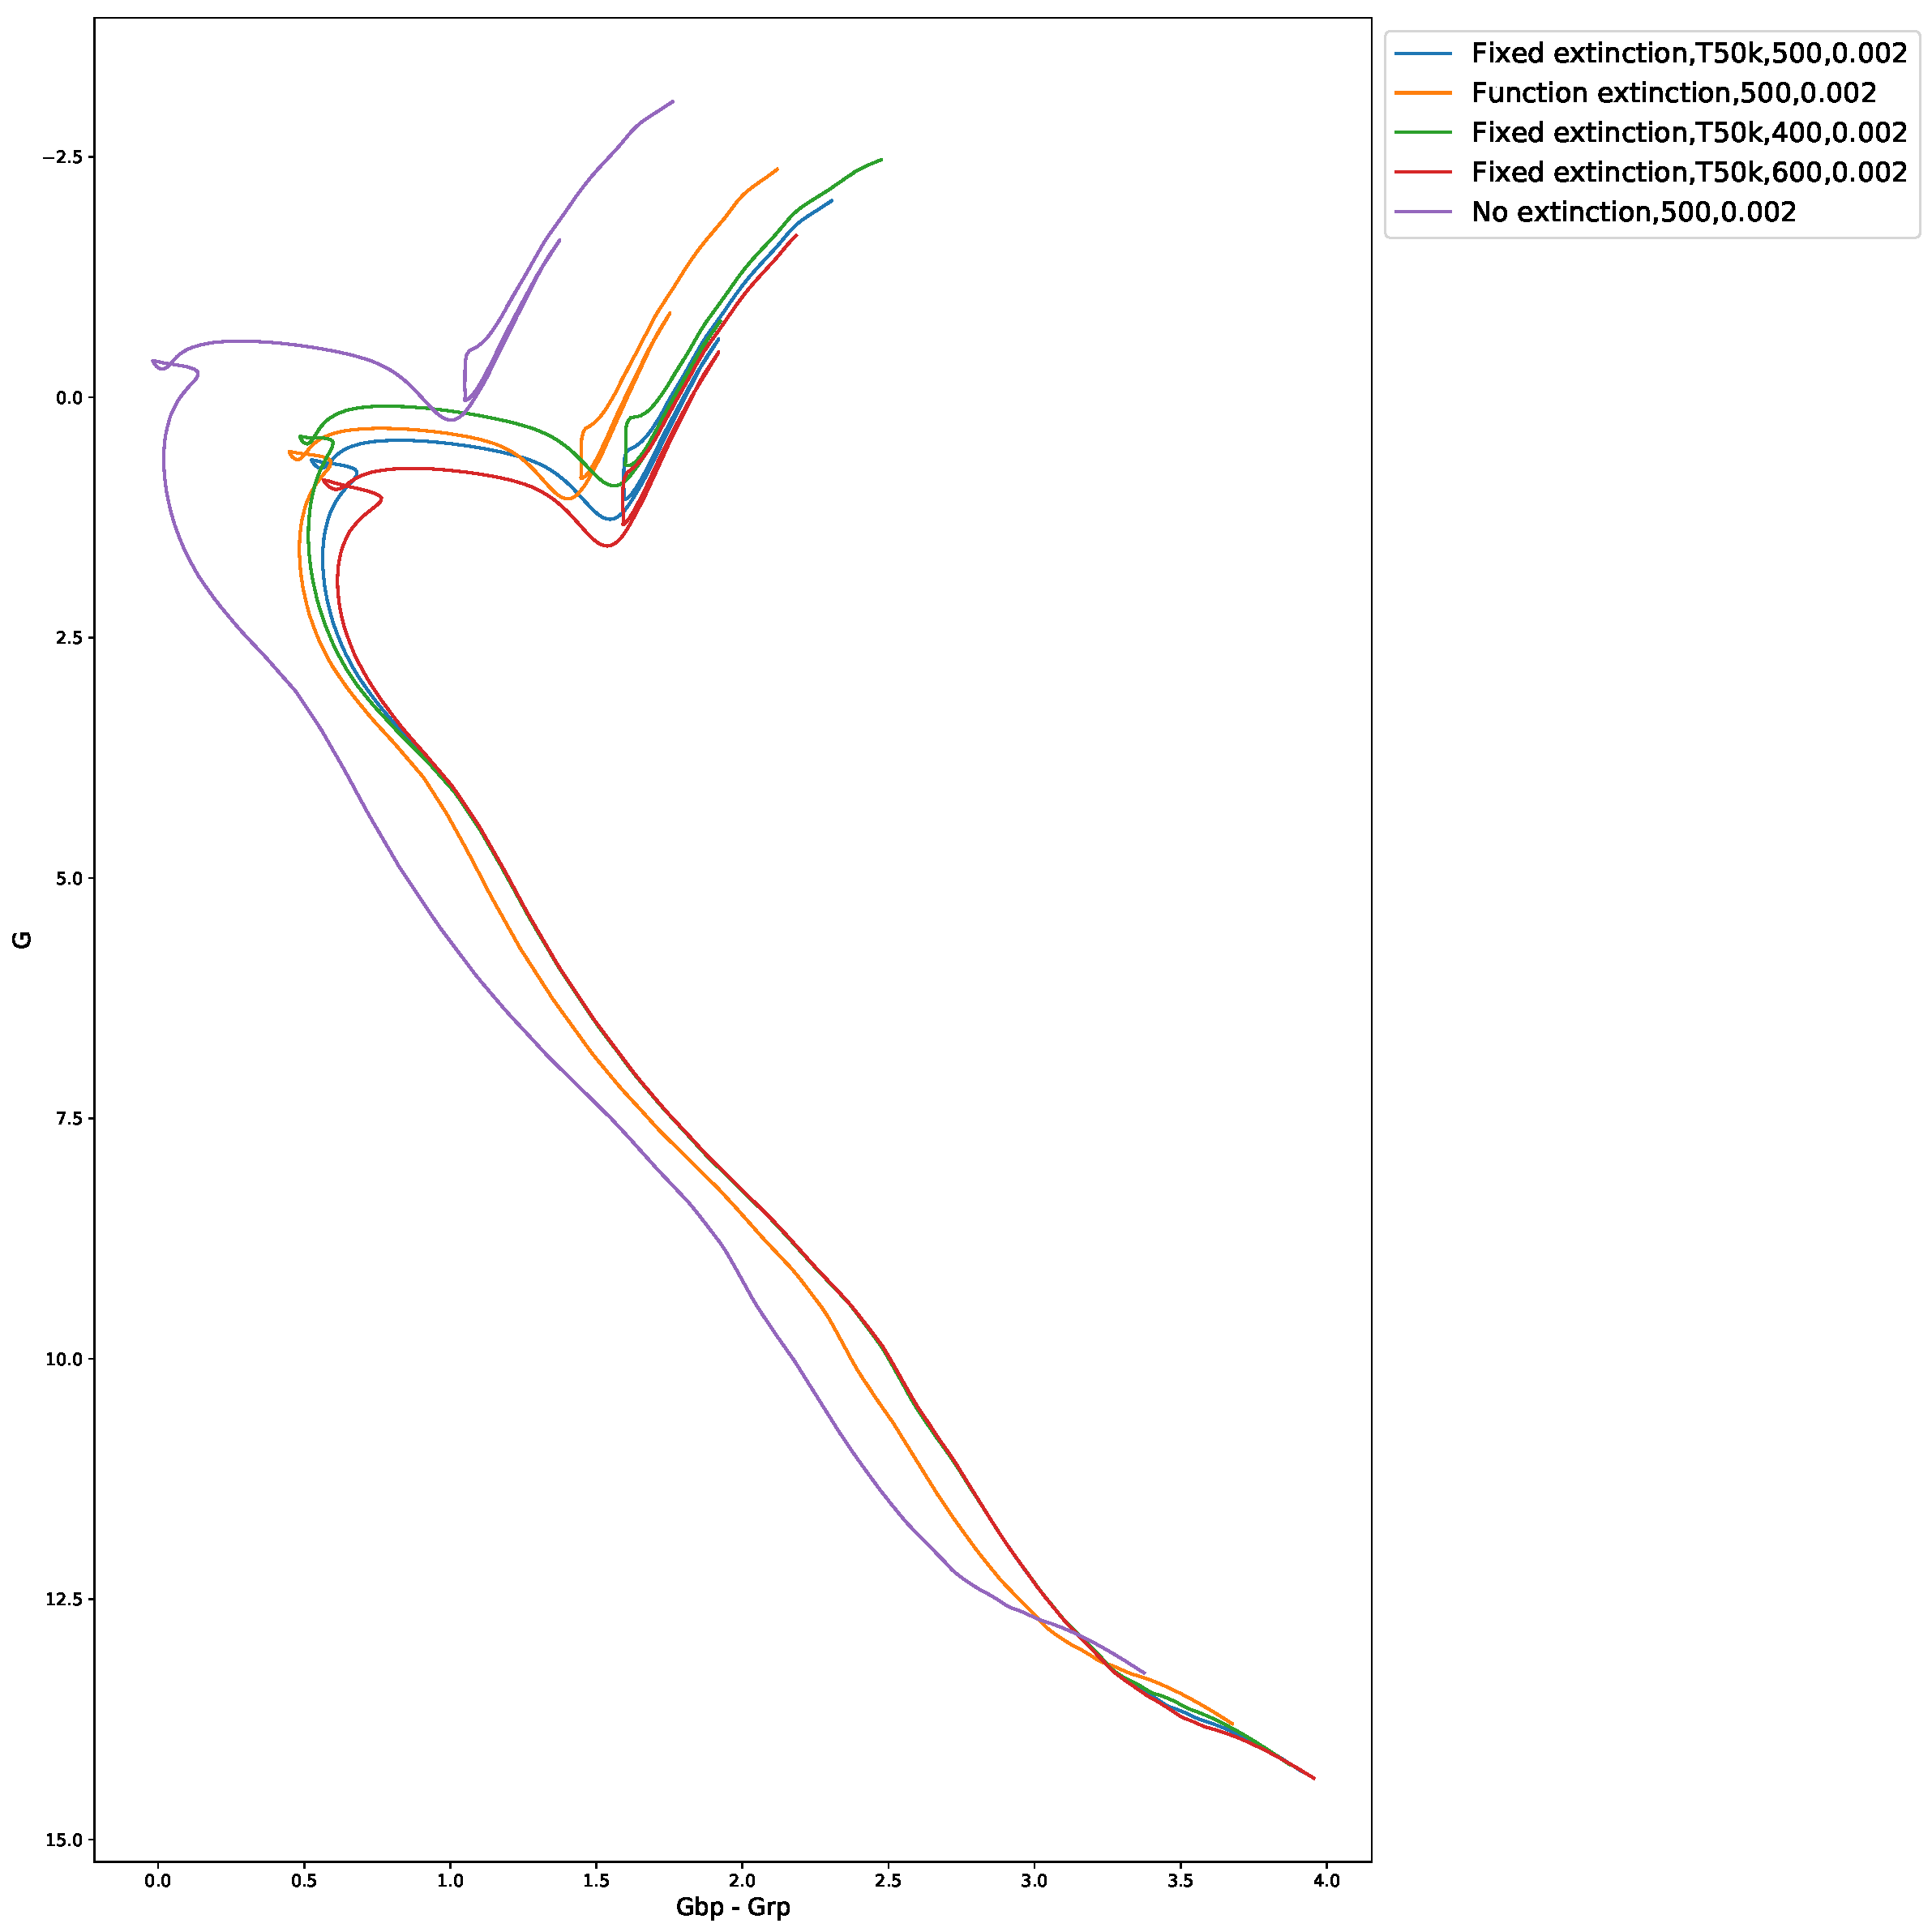
\includegraphics[width=1.0\textwidth]{../basti_isochrones_10_13Gyr/Extinction_T50k_FeH0fix_func_G_GbpmGrp_500_400_600_Myr_FeH_0p002_ref_noext_Av_1p0.pdf}
\caption{Gaia $G$-($G_{\textnormal{bp}}$-$G_{\textnormal{rp}}$) CMD with a fixed extinction value equal to $(A_{X}/A_{V})_{plat}$ for each filter}
\label{gaia_isoc_T50k}
\end{center}
\end{figure}

For the Gaia CMD, when $(A_{X}/A_{V})_{MS}$ is used for the fixed-extinction ratio isochrones, as shown in Figure \ref{gaia_isoc_T5k}, the turnoff position of the 500 Myr FBER isochrone appears to be lower on the main sequence than even the 600 Myr fixed-extinction case, suggesting that using the fixed-extinction treatment significantly and consistently over-estimates the isochrone age for an observed cluster. However, unlike the WFC3 F814W-(F275W-F814W) CMD, the alignment of the main sequence continues almost along the  entire MS length. \\*

When using $(A_{X}/A_{V})_{plat}$ for the fixed-extinction isochrones, the whole isochrone is significantly shifted down and to the right when moving from the FBER isochrone to the fixed-extinction isochrone, as can be seen in Figure \ref{gaia_isoc_T50k}. Since all four isochrones with added extinction in this figure assume that $A_{V} = 1.0$, alignment of the upper main sequences when using $(A_{X}/A_{V})_{plat}$ can only be achieved by having a lower value of $A_{V}$ for the fixed-extinction isochrones than for the FBER case. Depending on the exact value of the fixed $A_{X}/A_{V}$ used for fitting an isochrone to a given observed cluster, the resulting value calculated for $A_{V}$ and, subsequently, $E_{B-V}$ could be significantly underestimated. \\*

\section{NGC 6793} \label{ngc6793_res_disc}
\subsection{Effects of extinction treatment on isochrones}

Before comparisons between the GC18 results and those for a FBER-based fit can be made, a reference isochrone, with a globally-fixed $A_{V}$ value of 0.843 and age of 600 Myr (in accordance with the GC18 values in Table \ref{NGC6793_obs}), was created. This was done to test whether or not a BaSTI isochrone constructed according to the GC18 results could produce an accurate fit to the observational data. The $A_{X}/A_{V}$ values required for this isochrone to achieve alignment with the upper main sequence below the MSTO were equal to the $(A_{X}/A_{V})_{plat}$ values for each Gaia filter. While the results from GC18 do not include a metallicity estimate for NGC 6793, it can be estimated from its age that a solar-like metallicity is likely. Therefore, the relevant isochrone has a metallicity of [Fe/H] = 0. Due to the overall red-ward shift of an isochrone when treated with an extinction ratio of $(A_{X}/A_{V})_{plat}$, rather than the physically more-realistic $(A_{X}/A_{V})_{MS}$, as demonstrated in Figure \ref{gaia_isoc_T50k}, the GC18 parameter values, in particular the listed $A_{V}$ value of 0.843, do not produce an accurate fit when using the FBER treatment in the isochrones for the NGC 6793 observational data.\\*


\begin{figure}[h!]
\begin{center}
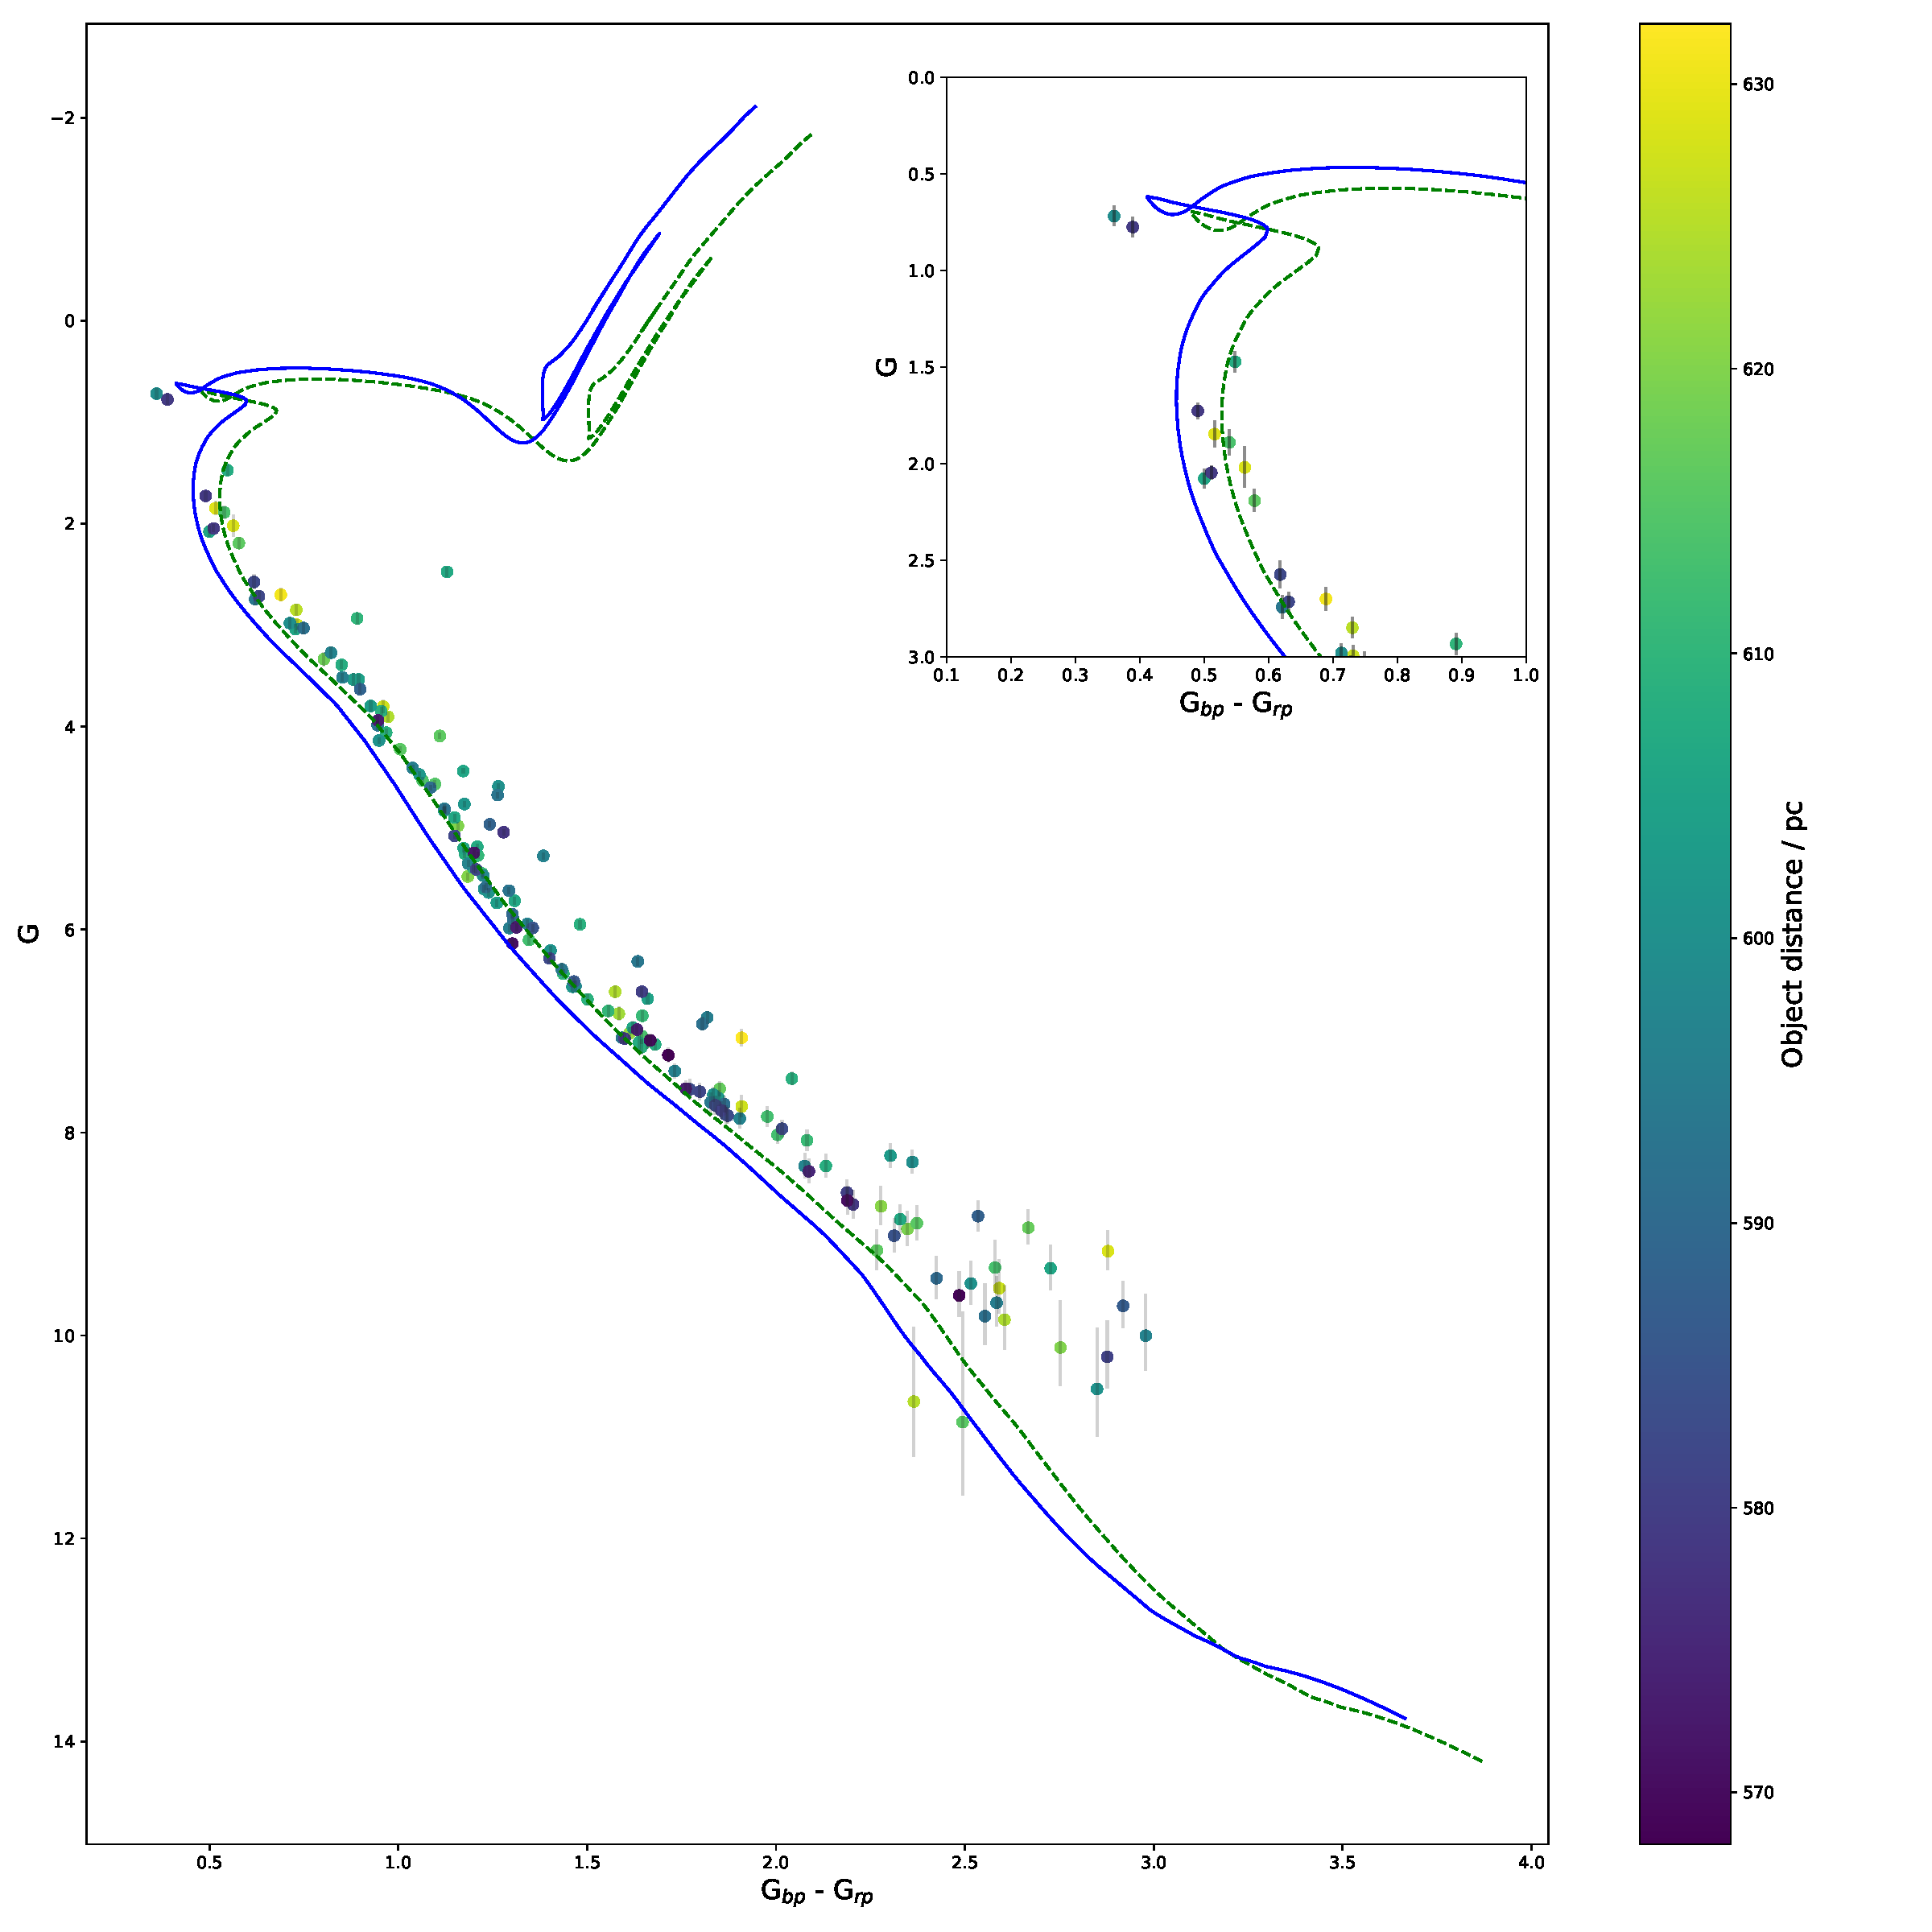
\includegraphics[width=1.0\textwidth]{../NGC_6793_CMD_FeH_0p002_Av_0p84_600Myr_isochrones_summary_errorbars.pdf}
\caption{FBER treatment (solid blue) and fixed-extinction ratio (dashed green) isochrones calculated using the GC18 cluster parameters, i.e., an age of 600 Myr, an $A_{V}$ value of 0.84 and solar metallicity.}
\label{NGC_6793_gc18_params_function}
\end{center}
\end{figure}

Using the cluster parameters determined by GC18 did not produce a satisfactory fit between the FBER isochrone and the observations. As shown in Figure \ref{NGC_6793_gc18_params_function}, the GC18 values produce an FBER isochrone whose MS lies too far beyond the blue colour-index range of the MS and thereby does not align with the position of the MSTO either, necessitating a higher value of $A_{V}$ to increase the predicted colour index of the isochrone. The metallicity had to be increased in order to realign the FBER and fixed-extinction isochrones in the lower main sequence. After this, the age of the FBER isochrone needed to be lowered in order to realign the MSTO positions of the two isochrones.\\*

\begin{figure}[h!]
\begin{center}
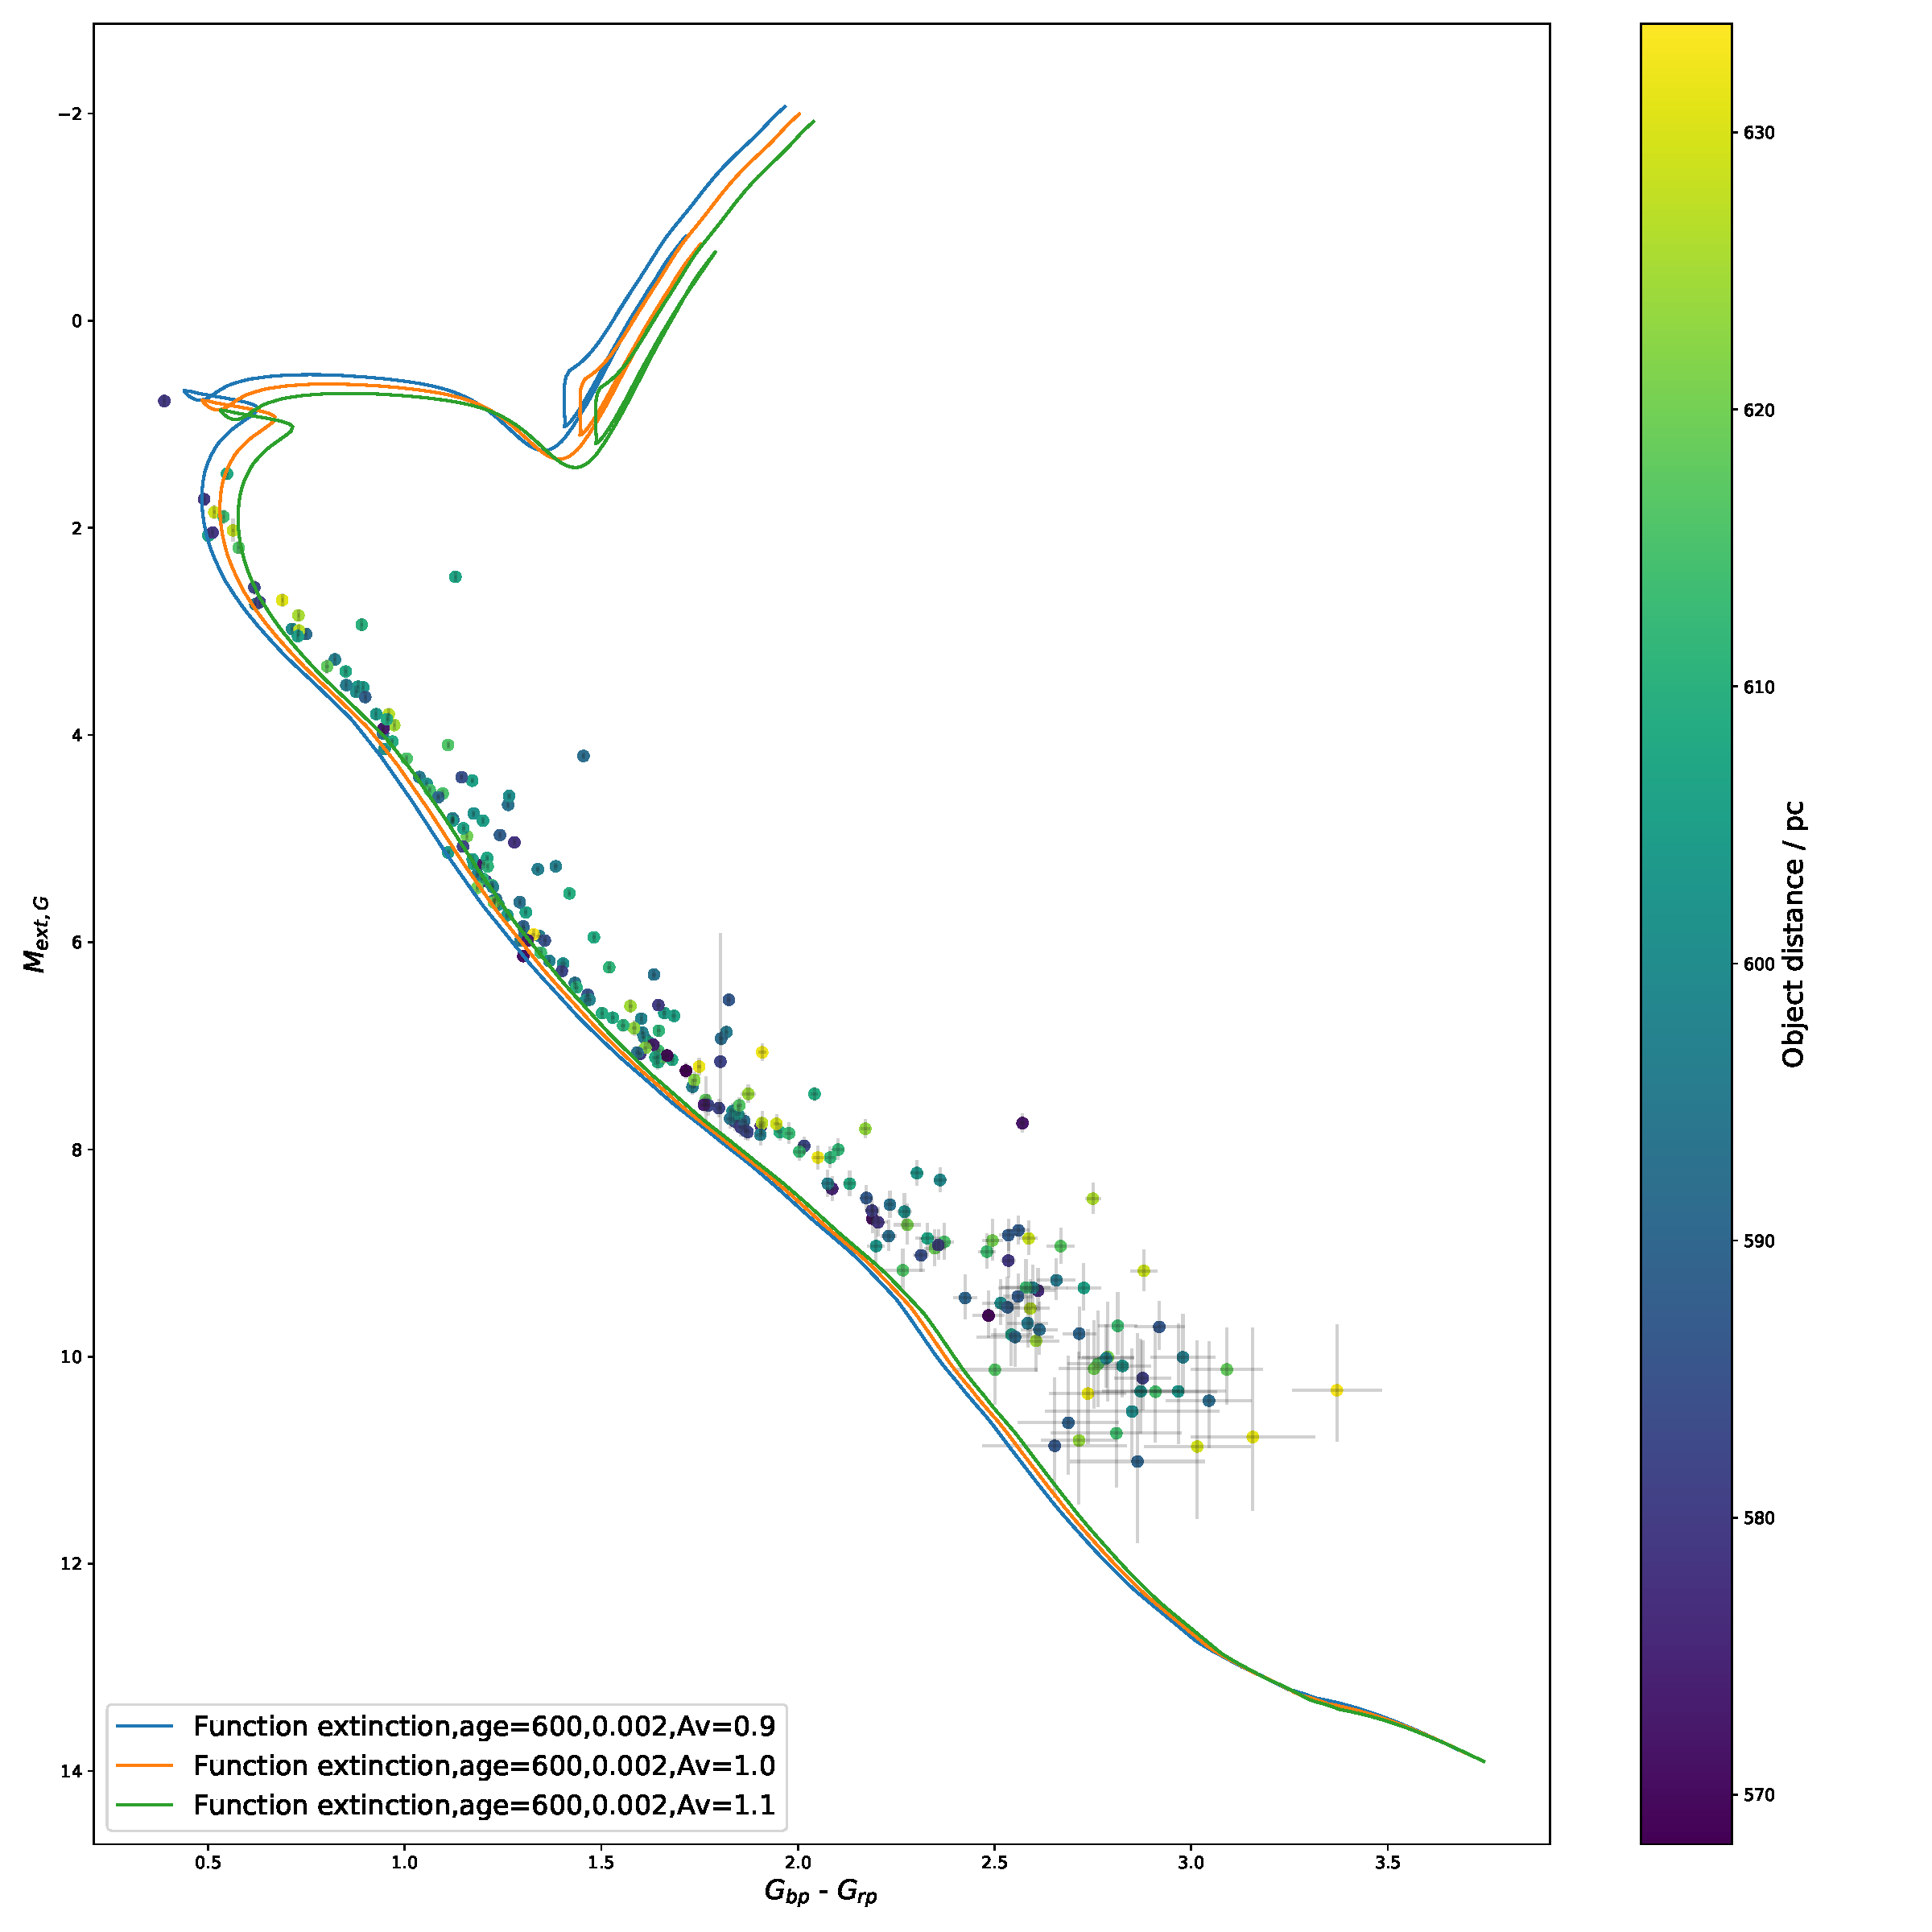
\includegraphics[width=1.0\textwidth]{../NGC_6793_CMD_FeH_0p002_Av_0p9_1p0_1p1_600Myr_isochrones_func_errorbars_T5k.pdf}
\caption{Illustration of the effect in the Gaia CMD of changing the value of $A_{V}$ used in the calculation of the FBER models applied to isochrones. The observed CMD of NGC 6793 is plotted, together with three FBER isochrones, all with ages of 600 Myr and solar metallicity. The curves have $A_{V}$ values of 0.9 (orange), 1.0 (green) and 1.1 (blue), respectively.}
\label{NGC_6793_Av_var}
\end{center}
\end{figure}

\begin{figure}[h!]
\begin{center}
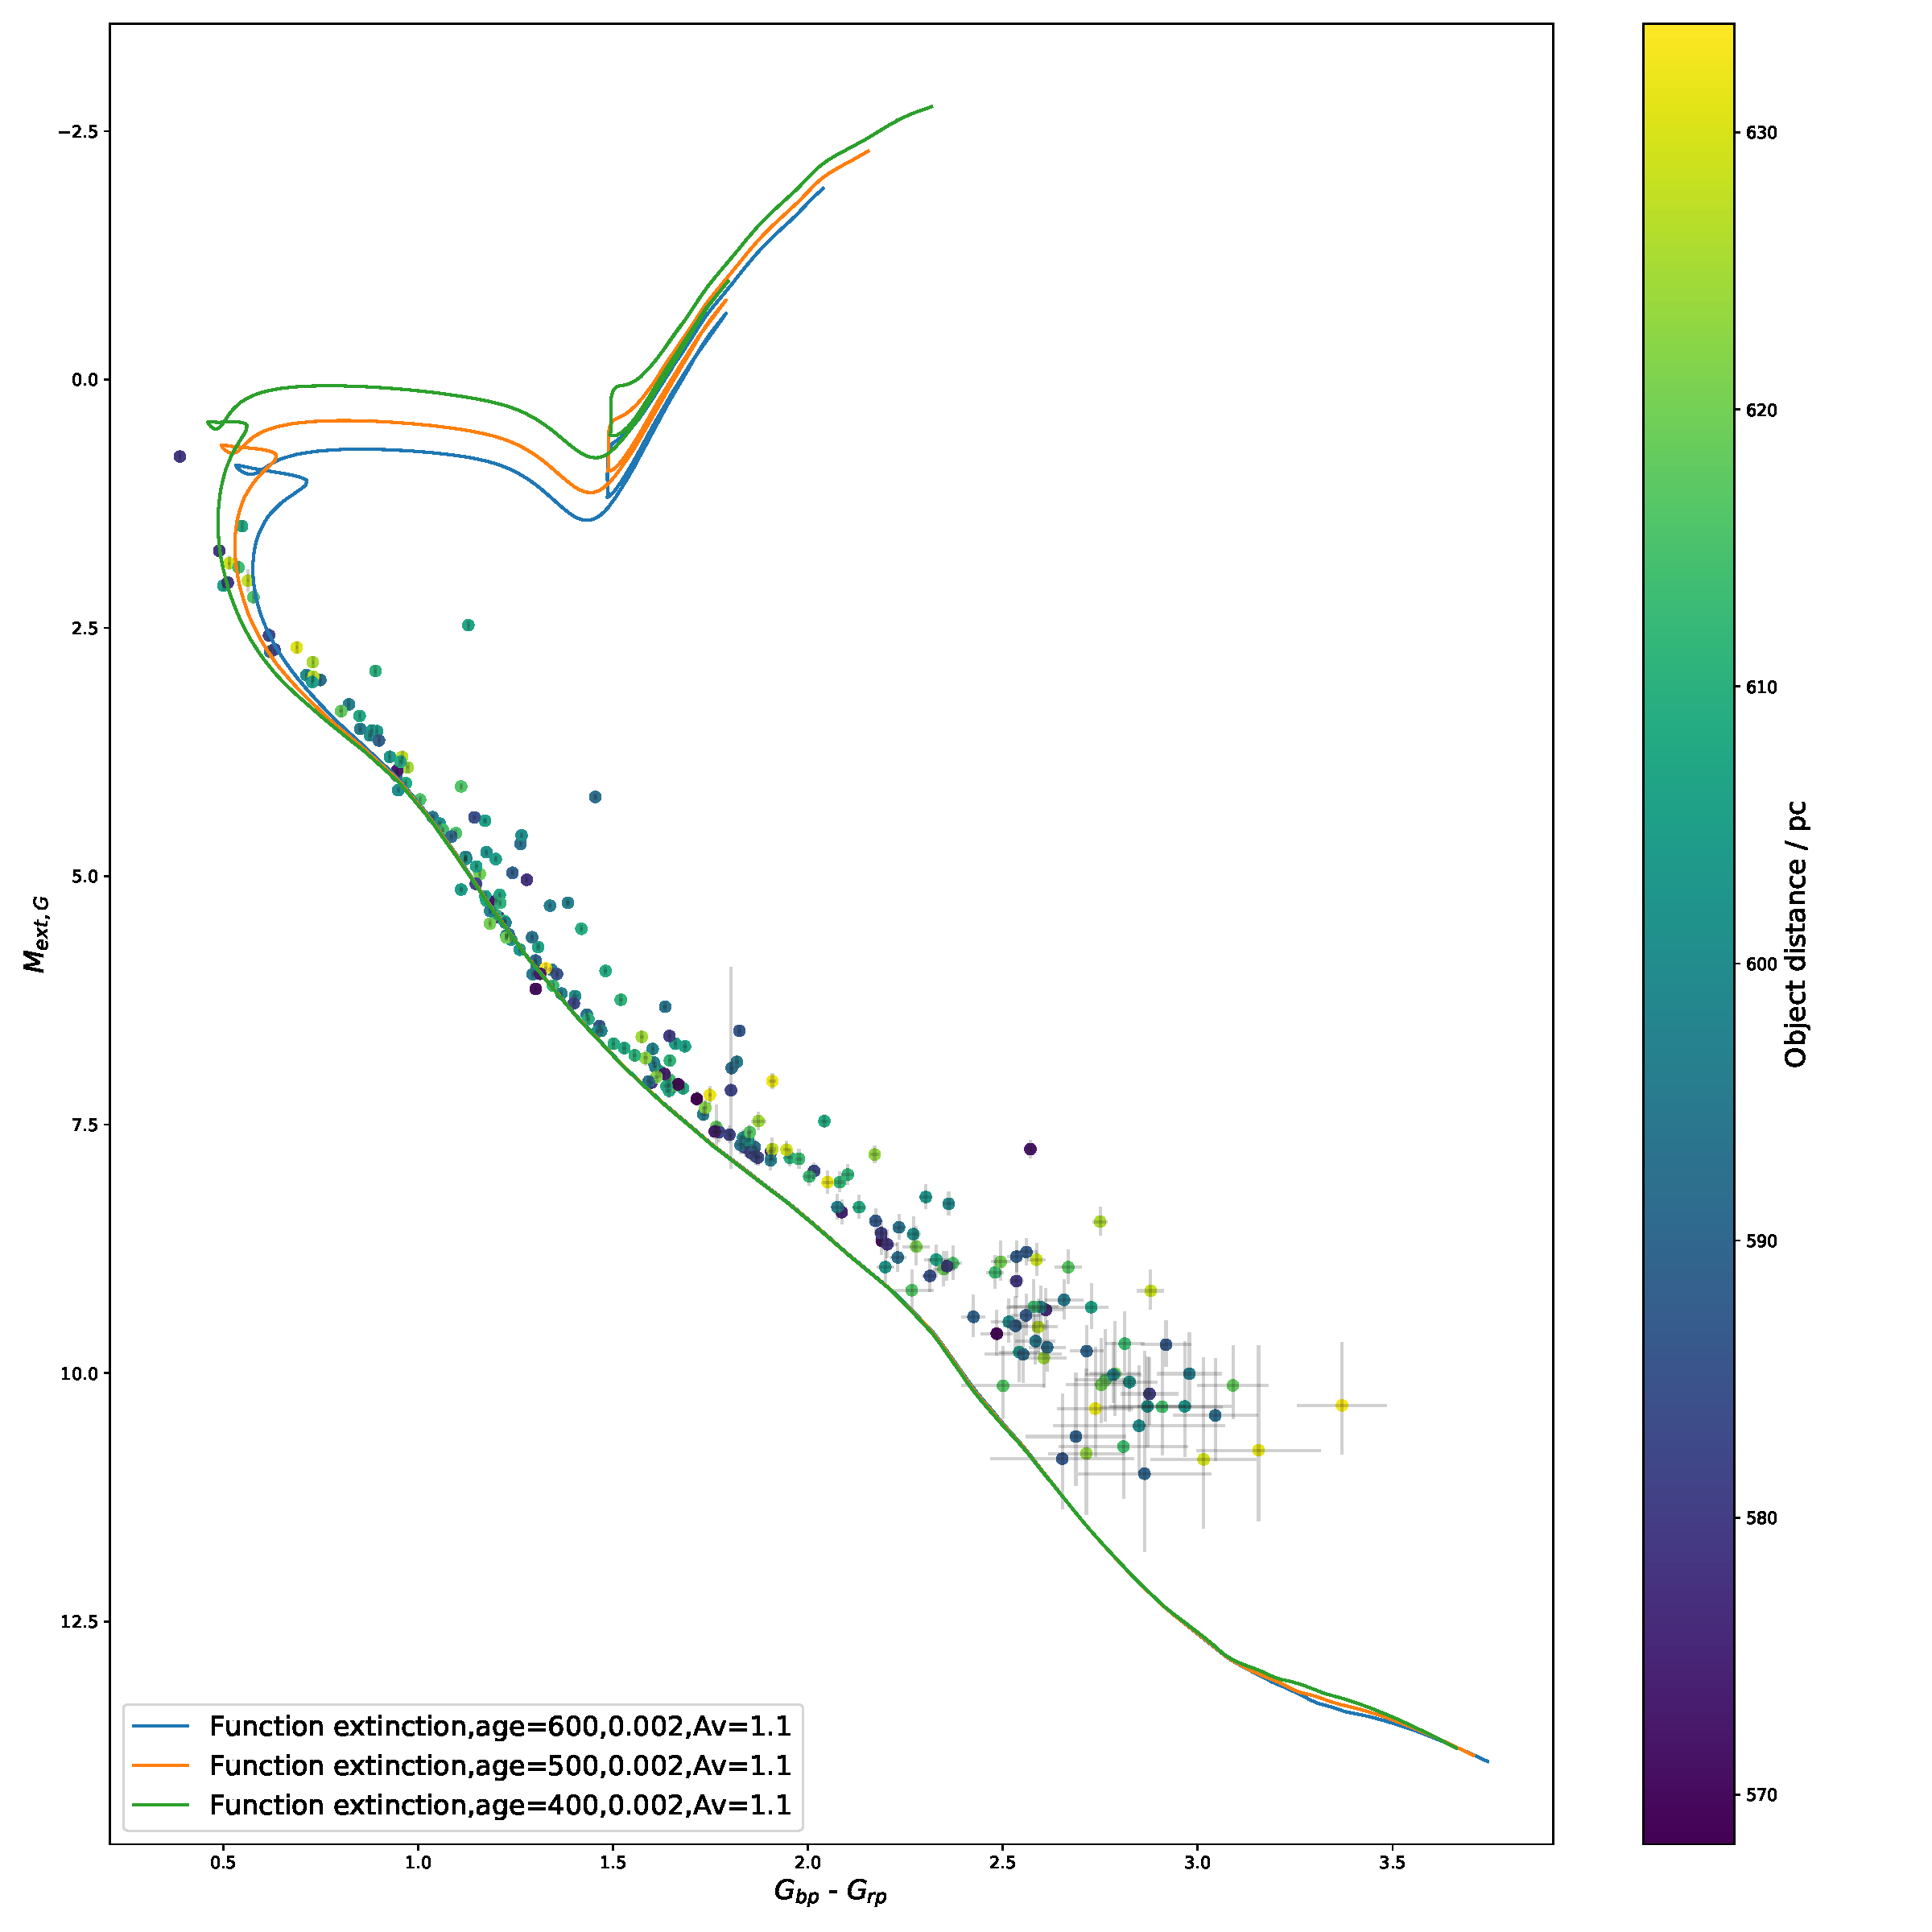
\includegraphics[width=1.0\textwidth]{../NGC_6793_CMD_FeH_0p002_Av_1p1_600_500_400Myr_isochrones_func_errorbars_T5k.pdf}
\caption{Illustration of the effect in the Gaia CMD of changing the age of an isochrone. The observed CMD of NGC 6793 is plotted, together with three FBER isochrones, all with an $A_{V}$ value of 1.1 of and solar metallicity. The curves have ages of 400 (green), 500 (orange) and 600 (blue), respectively.}
\label{NGC_6793_age_var}
\end{center}
\end{figure}

\begin{figure}[h!]
\begin{center}
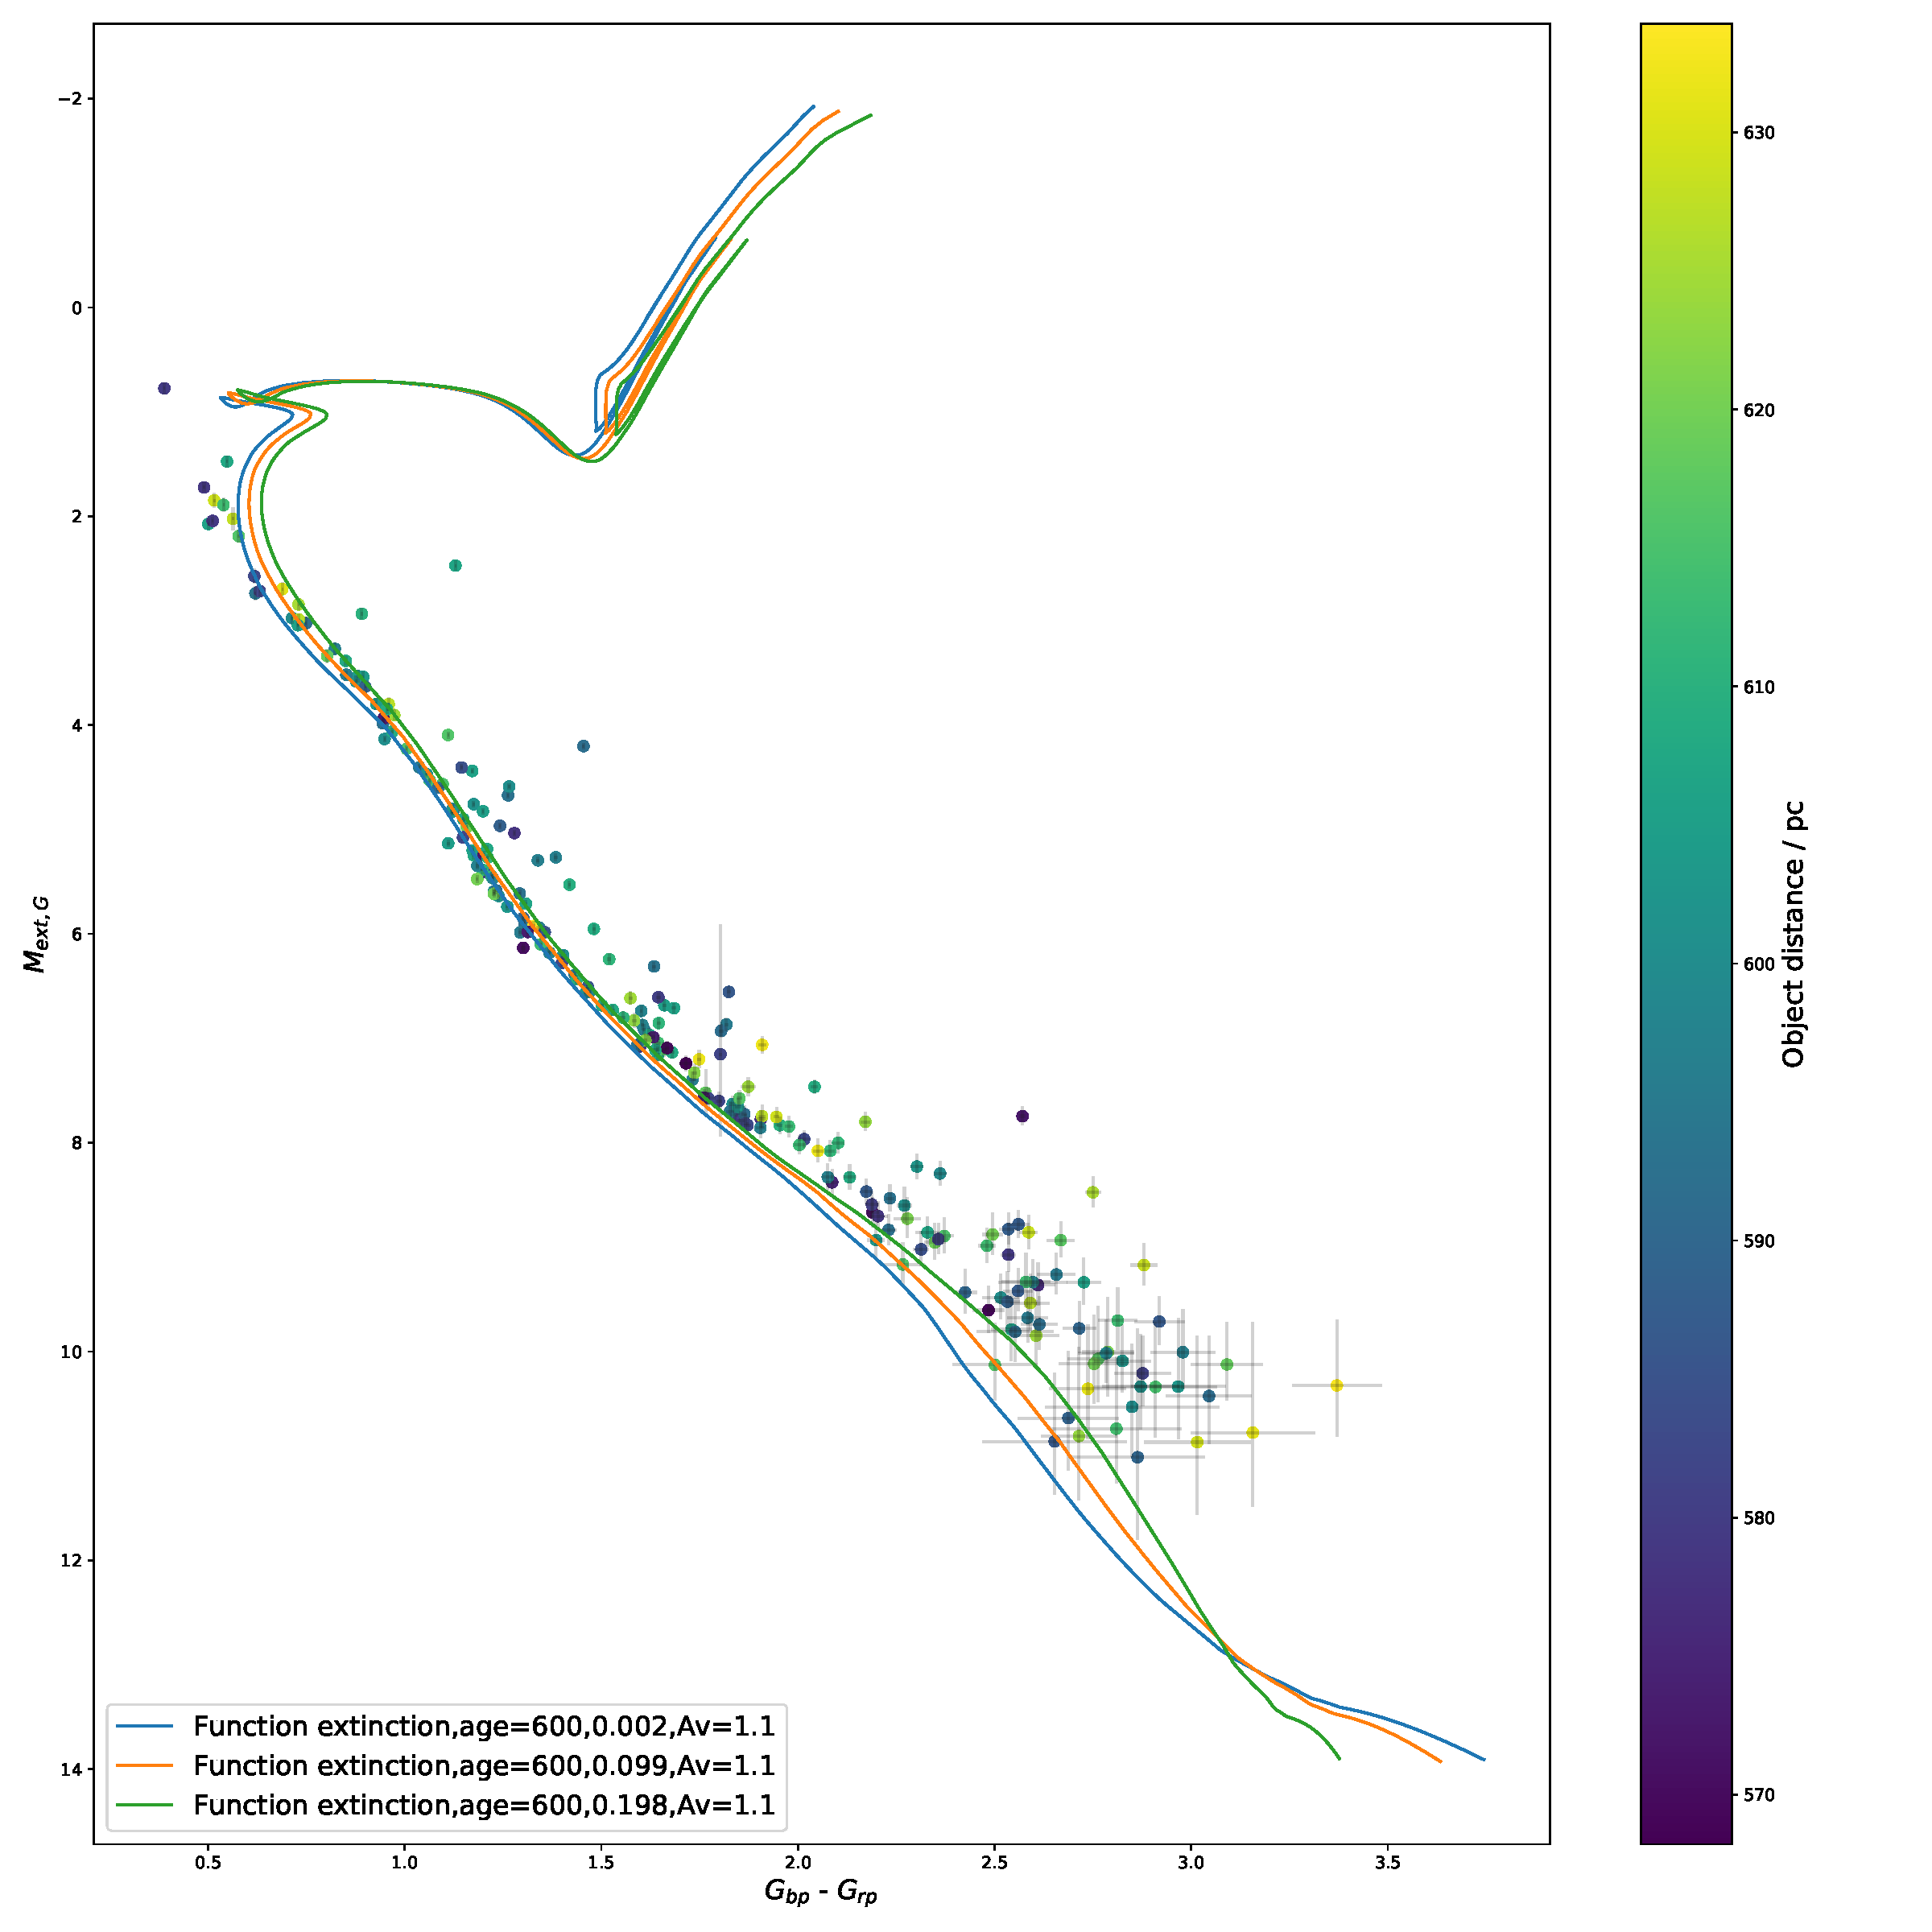
\includegraphics[width=1.0\textwidth]{../NGC_6793_CMD_FeH_0p002_0p099_0p198_Av_1p1_600Myr_isochrones_func_errorbars_T5k.pdf}
\caption{Illustration of the effect in the Gaia CMD of changing the metallicity of an isochrones. The observed CMD of NGC 6793 is plotted, together with three FBER isochrones, all with ages of 600 Myr and an $A_{V}$ value of 1.1. The curves have [Fe/H] values of 0.0 (blue), 0.1 (orange) and 0.2 (green), respectively.}
\label{NGC_6793_metal_var}
\end{center}
\end{figure}


Before making an age estimate, the main sequence of the FBER isochrone had to align with the MS of NGC 6793. It was found that the positions of MS objects in the region $1.0 \lesssim (G_{\textnormal{bp}}-G_{\textnormal{rp}}) \lesssim 1.5$, well below the MSTO, varied the least with changes in metallicity for the FBER isochrone, as shown in Figure \ref{NGC_6793_metal_var}. By contrast, changing the $A_{V}$ value applied to the isochrone produced a more homogeneous shift in positions along the entire isochrone, as would be expected. The effect of changing between $A_{V}$ values is shown in Figure \ref{NGC_6793_Av_var}, in which it can be seen that the shift is much more uniform along the length of the main sequence below the MSTO region than the MS shifts between different metallicity values shown in Figure \ref{NGC_6793_metal_var}. Therefore, the initial alignment of this region was achieved by placing greater importance on the isochrone $A_{V}$ value than on the metallicity. The metallicity variations were then used to align the remaining regions of the MS with the observed data. Finally, isochrones of different ages were plotted to determine the best-fit cluster age, since the age has no significant effect on the isochrone position below the MSTO, as shown in Figure \ref{NGC_6793_age_var}. \\*

The alignment of the MS region described above for a FBER treatment was achieved using a value of $A_{V} = 1.1$. To better align the FBER isochrones to the lower main sequence, an increase in isochrone metallicity was required. The best-fit metallicity value was found to be [Fe/H] = 0.062. However, the magnitudes of the observational errorbars in $M_{\textnormal{ext},G}$ for lower MS stars (see Figure \ref{NGC_6793_obs_only}) dwarf any isochrone position changes due to changing metallicities between extinction treatments in the main sequence. Once these parameters were determined, the FBER isochrone with the best-fitting MSTO position had an age of 500 Myr, which is lower than the GC18 estimate of 603 Myr, as shown in Table \ref{NGC6793_result}. \\*


\begin{table}
\begin{center}
\begin{tabular}{ccccc}
\hline
Cluster property & K05 & K13 & GC18 & This project \\
\hline
Age / Myr & 437 & 495 & 603 & 500 \\
$A_{V}$ / mag & 0.53 & 0.967 & 0.843 & 1.1 \\
$\textnormal{[Fe/H]}$ & ? & ? & ? & 0.062 \\
Members & ? & 133 & 271 (photometric) & 231 \\
\hline
\end{tabular}
\caption{Comparison of results from this project with results of previous studies of NGC 6793.}
\label{NGC6793_result}
\end{center}
\end{table}

It can be seen that the age estimate made for the FBER isochrone in this project is similar to that made by K13, shown in Tables \ref{NGC6793_obs} and \ref{NGC6793_result}. However, the result for the FBER isochrone for this project was achieved using a different set of observation data from that of K13, which used data from the PPMXL and 2MASS catalogues. The FBER results also predict a higher cluster $A_{V}$ value than K13. Furthermore, the distance to the cluster was estimated at 724 pc by K13, using photometric data from the \cite{2010arXiv1012.3224H} catalogue. Meanwhile the observed Gaia dataset presented by GC18 contains parallaxes, whose values are independent of source brightness, for both the individual stellar members and the cluster as a whole. The GC18 points strongly to a cluster distance of 601 pc, which differs significantly from the 724 pc value predicted by K13. Finally, the K13 estimates were made using the fixed-extinction assumption, while the estimates made in this project using the FBER approach, introducing another source of uncertainty when comparing the two. In summary, the resemblance between the results for the FBER isochrones and the K13 results is likely to be superficial rather than proof that the results of the FBER approach do not differ significantly from those of the fixed-extinction approach.\\*

\begin{figure}[h!]
\begin{center}
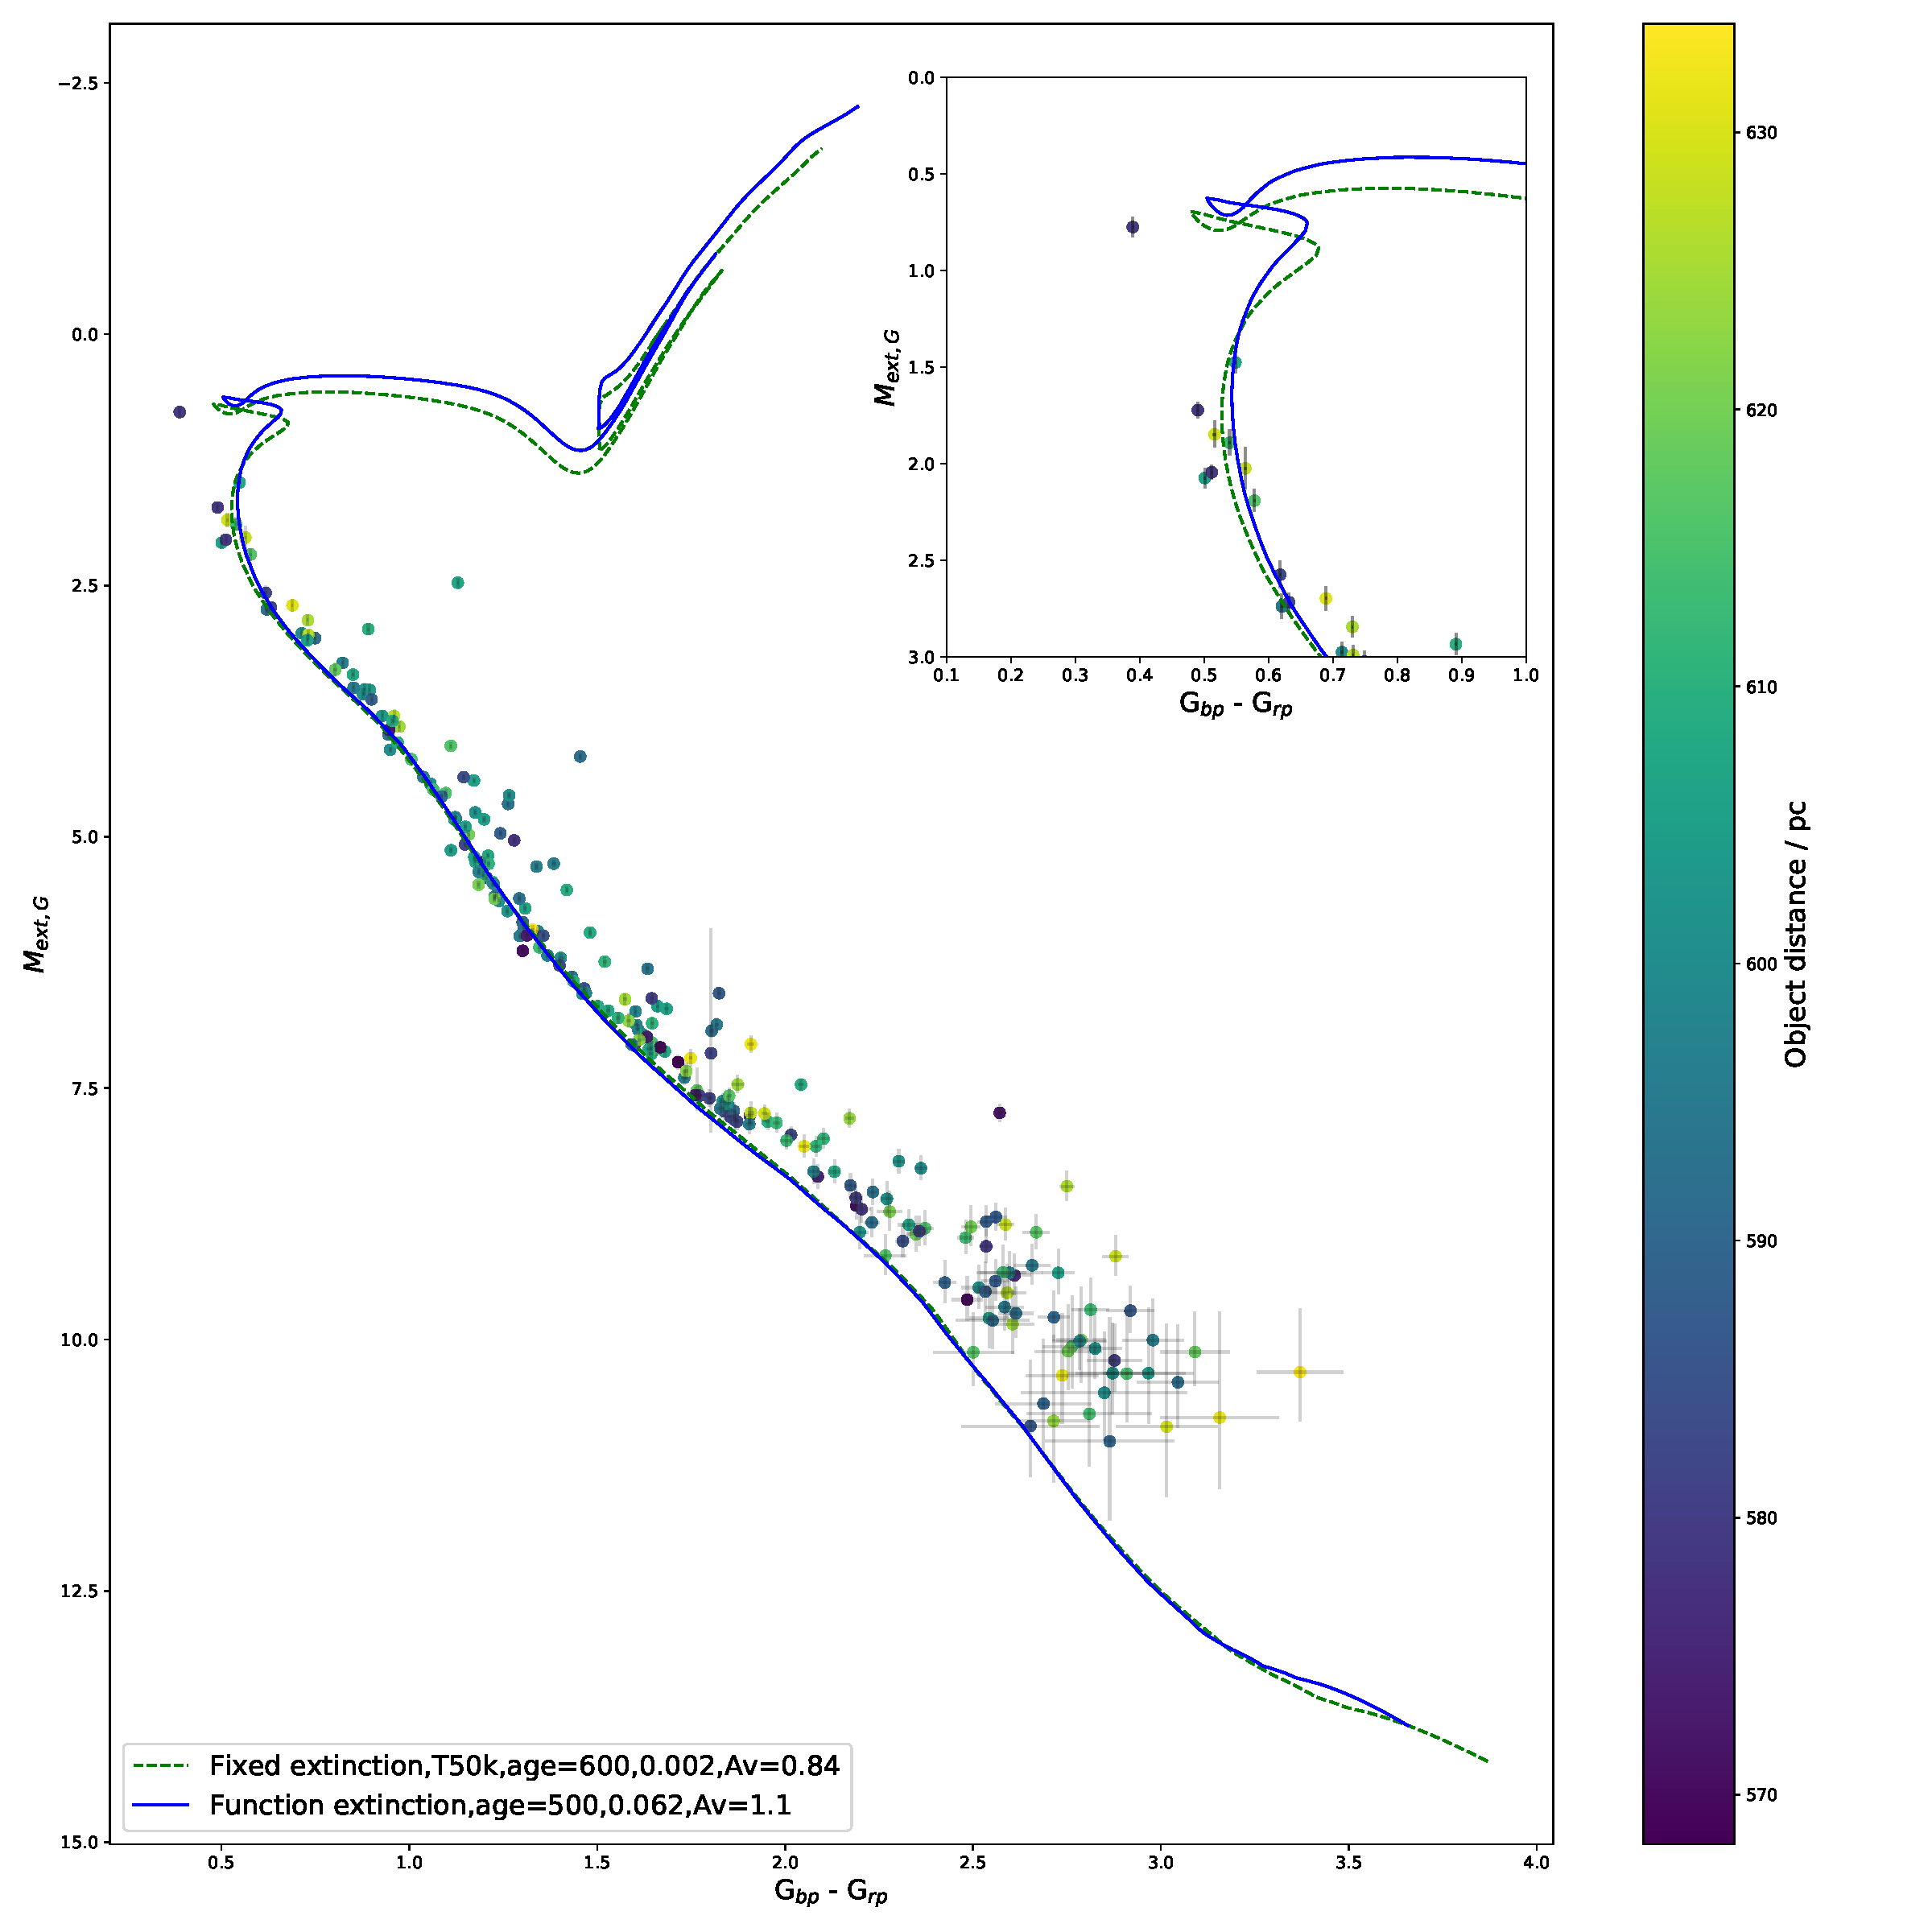
\includegraphics[width=1.0\textwidth]{../NGC_6793_CMD_FeH_0p062_Av_1p1_500Myr_vizier_isochrones_summary_errorbars.pdf}
\caption{Gaia $G$-($G_{\textnormal{bp}}$-$G_{\textnormal{rp}}$) CMD of NGC 6793, showing the 231 distance-corrected cluster members in the final dataset overlaid with a isochrone treated with a fixed extinction-ratio value of $(A_{X}/A_{V})_{plat}$ and age, $A_{V}$ and [Fe/H] values taken from the GC18 results in Table \ref{NGC6793_obs} and a 500-Myr FBER isochrone (solid blue) with an $A_{V}$ value of 1.1 and a metallicity of [Fe/H] = 0.062, with observational errorbars added. The inset panel shows a zoomed-in view of the MSTO region.}
\label{NGC_6793_isoc_inset_1.1_500_0.062}
\end{center}
\end{figure}

\subsection{Sources of uncertainty}
\subsubsection{Observational data errors}


The final Gaia observational sample of stars in NGC 6793 is shown as a distance-corrected CMD in Figure \ref{NGC_6793_obs_only}, with distances and photometric errors propagated directly from parallax measurements.\\*

The uncertainties in the parallax data for objects assigned to NGC 6793 were significantly higher for stars in the lower main sequence than elsewhere. This is to be expected, since stars in the lower main sequence are the faintest objects in the data and therefore are the most difficult to track against background sources.  This leads to uncertainties in the predicted $M_{\textnormal{ext},G}$ magnitudes, which are calculated by rearranging Equation \ref{ext_def_app_mag}. The parallax-derived errors on the ($G_{\textnormal{bp}}-G_{\textnormal{rp}}$) colour index are zero, as an object's colour index can simply be calculated as the difference between its apparent magnitudes in both filters, and is therefore independent of the object's parallax. For all stars, the photometric errors derived from parallax errors were also found to be much greater than errors in the photometric measurements themselves, as shown in the observational CMD (where the colour index scale is significantly smaller than the $M_{\textnormal{ext},G}$ scale on the axis labels). Again, this is not surprising as it is more difficult to precisely track single stars moving across the background sky than it is to precisely measure their observed brightness.\\*

The observational uncertainties for stars outside the lower MS region were found to be too small to resolve the difference between the positions of FBER and fixed-extinction isochrones treatments with the same cluster parameters, as shown in Figure \ref{NGC_6793_gc18_params_function}. Therefore, the difference between extinction treatments is significant with respect to observational uncertainties.

\subsubsection{FBER model errors}

\begin{figure}[h!]
\begin{center}
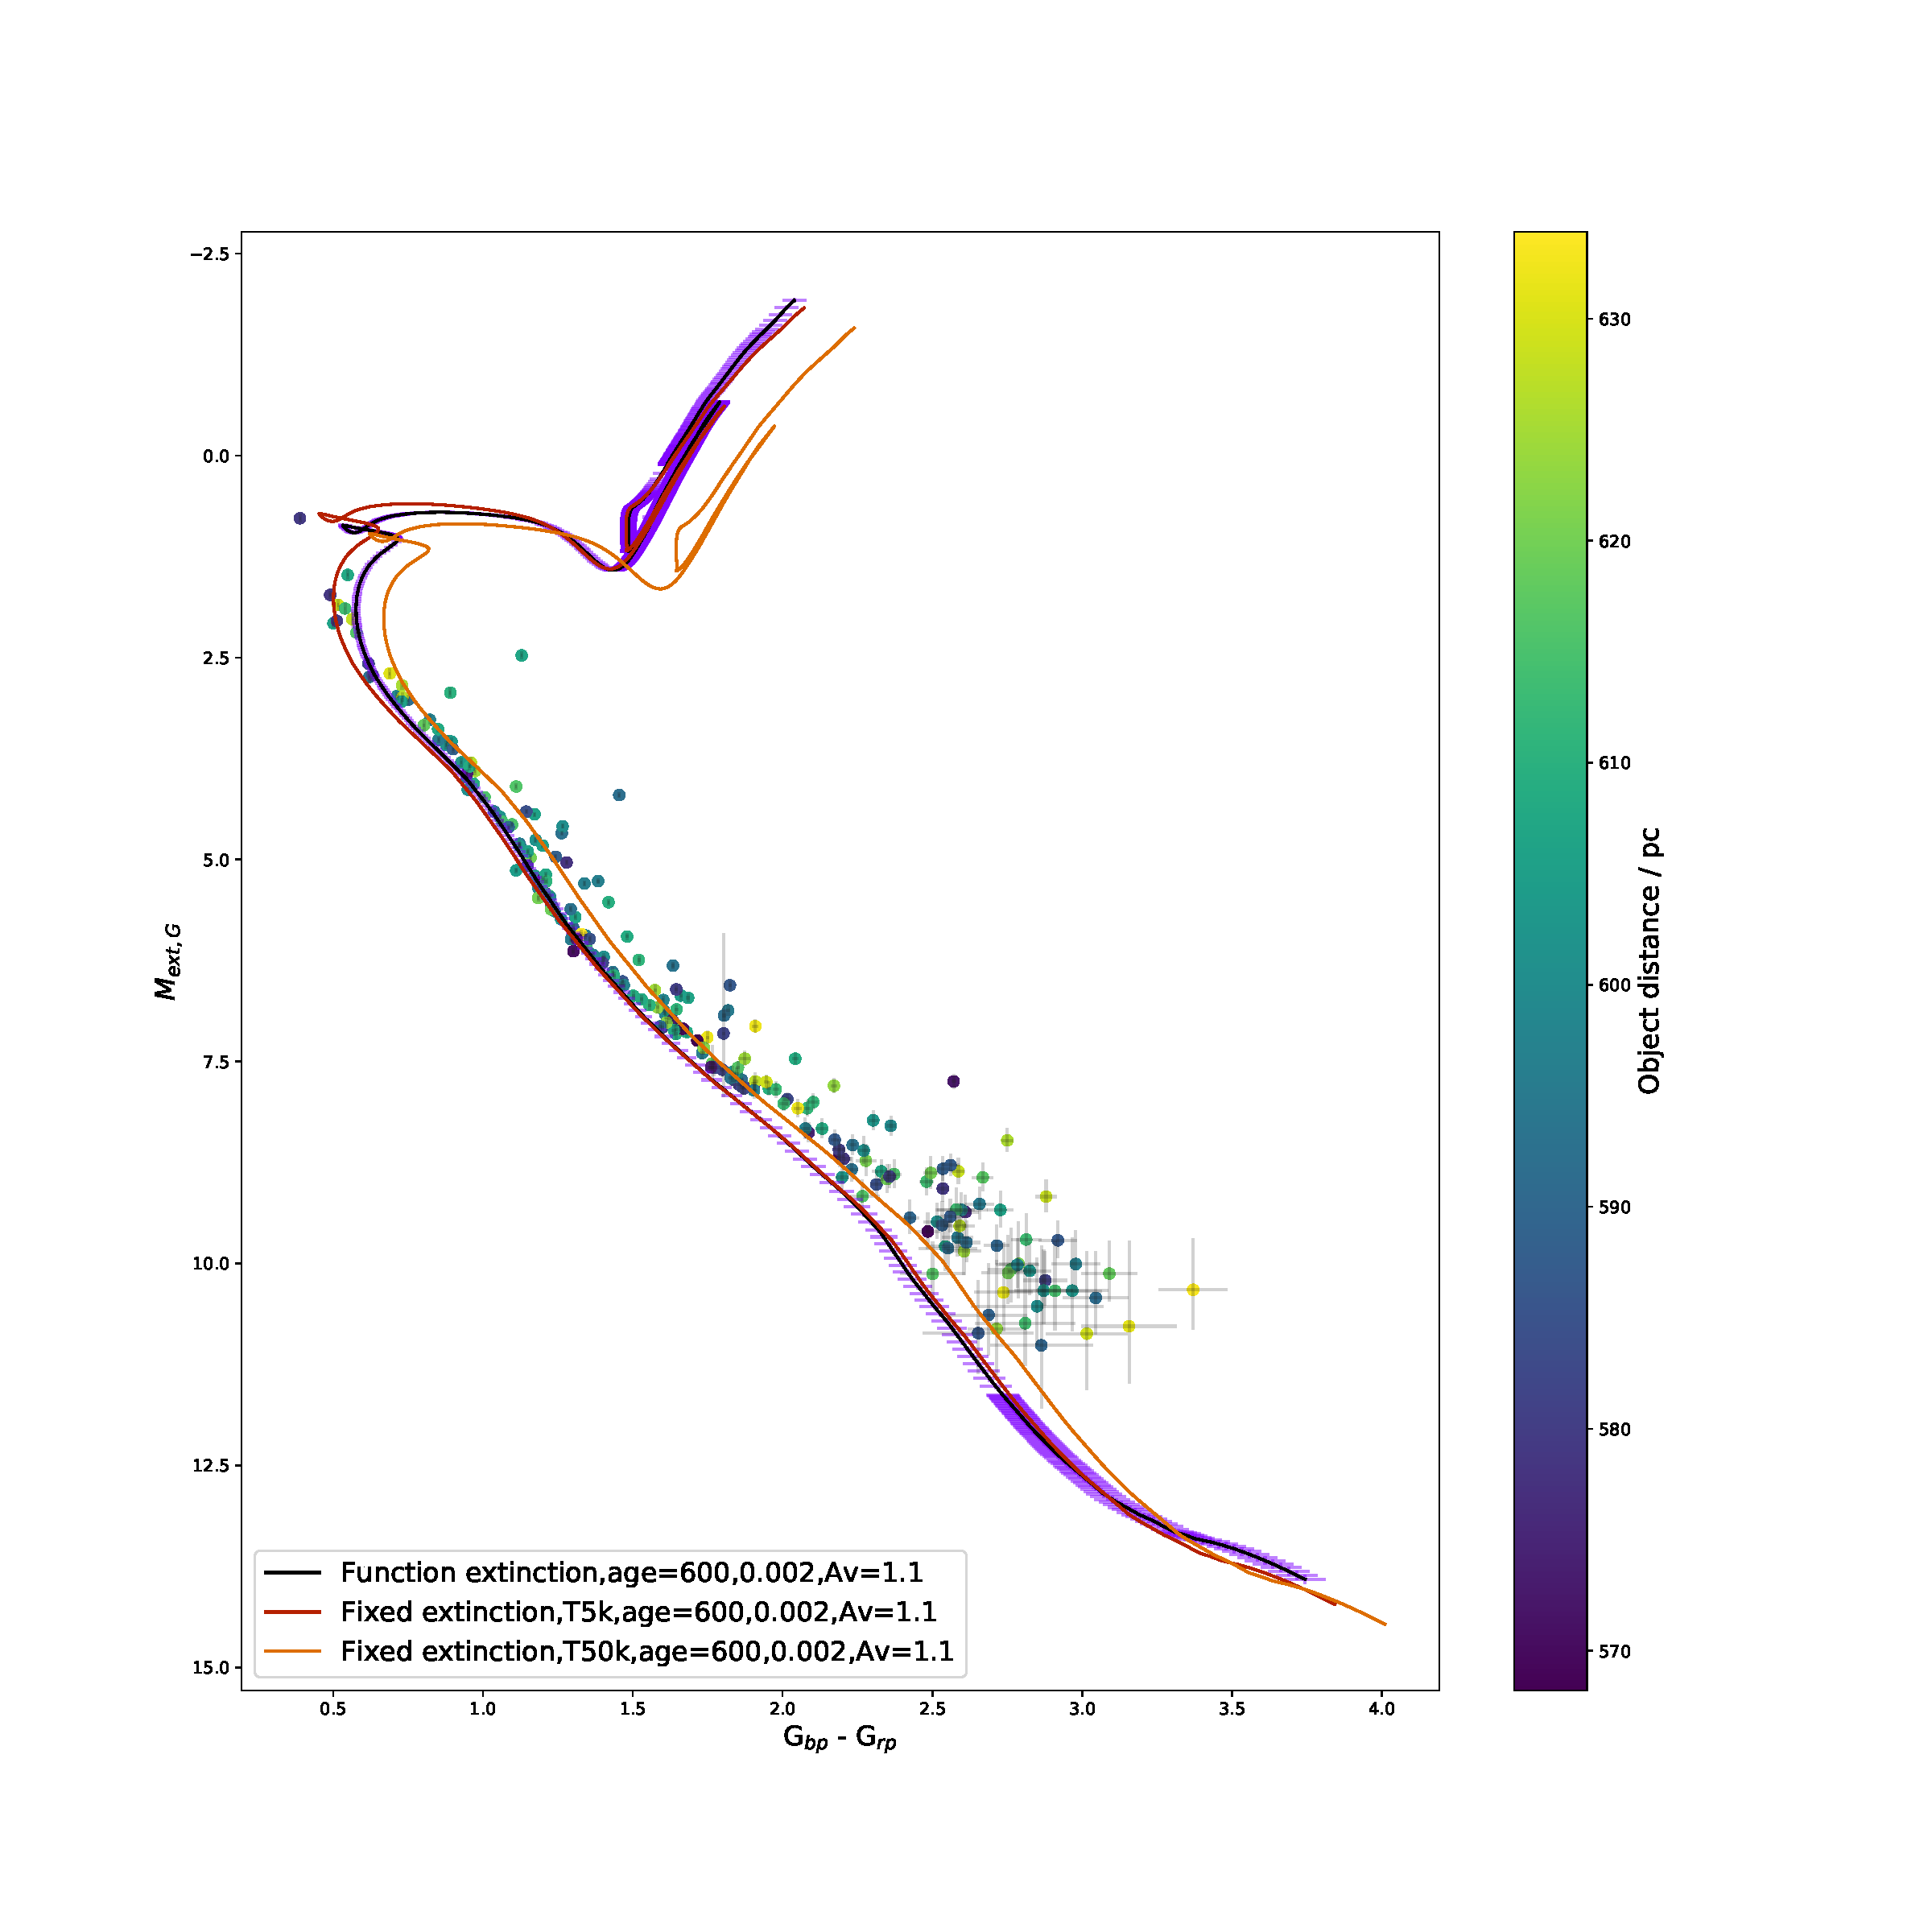
\includegraphics[width=1.0\textwidth]{../NGC_6793_CMD_Myr_model_err_vizier.pdf}
\caption{Observed CMD of NGC 6793, with three extinction scenario cases plotted over the observed data. All three isochrones have the same cluster parameter values, as shown in the legend. The curve treated using the FBER models introduced in this project is shown in black. The uncertainties in these models, whose calculation is briefly described in the text, are shown in both axes via the purple errorbars. The fixed-extinction models generated using $(A_{X}/A_{V})_{plat}$ and $(A_{X}/A_{V})_{MS}$ are shown in light orange and brown, respectively.}
\label{AxAv_model_err}
\end{center}
\end{figure}

The uncertainties in coefficient values for the $A_{X}/A_{V}$ models introduced in Section \ref{ext_models} could have an impact on the significance of changing extinction treatment methods - if sufficiently large, they could render the FBER approach unnecessary. As shown in Tables \ref{simpfunc_coeffs_table} and \ref{UV_coeffs_table}, uncertainties in the models are quantified as errors in the fitted coefficient values. These errors were propagated, using the standard error-propagation formula of partial derivatives with respect to each coefficient, to produce an estimate for the errors in $A_{X}/A_{V}$ for these models. Since each photometric filter has an independently-fitted function with different coefficients and errors, each of the three filters used for the Gaia CMD has an associated FBER model error. For the ($G_{\textnormal{bp}}-G_{\textnormal{rp}}$) axis, the error in the extinction ratio for the colour index was obtained by adding the individual filters' uncertainties in quadrature.\\*

Once the FBER error estimates for $M_{\textnormal{ext},G}$ and ($G_{\textnormal{bp}}-G_{\textnormal{rp}}$) were obtained, they were applied to the isochrone dataset and the results were plotted as errorbars centred on the FBER isochrone, as shown in Figure \ref{AxAv_model_err}. Errorbars were chosen over the shading of regions within the 1$\sigma$ uncertainty range because of complications in the RGB-HB-AGB region which resulted in incorrect shading in those regions.\\*

From the errorbars in Figure \ref{AxAv_model_err}, it is clear that the differences in cluster parameters resulting from the use of different extinction treatment methods, as summarised in Table \ref{NGC6793_result}, cannot be reconciled even when considering the uncertainties in both the observational data and the empirical $A_{X}/A_{V}$ models. \\*

\subsubsection{Selection of cluster members}

\begin{figure}[h!]
\begin{center}
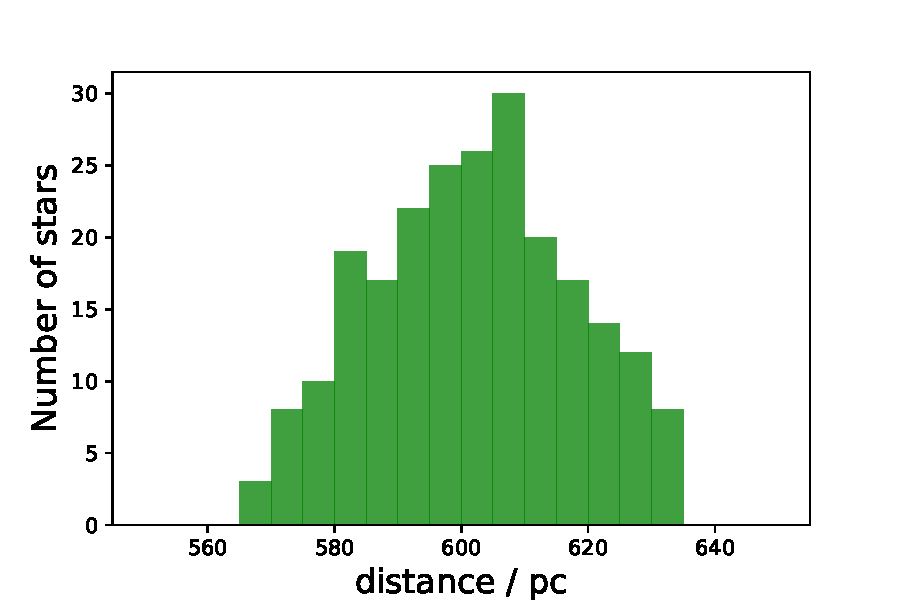
\includegraphics[width=1.0\textwidth]{../NGC_6793_vizier_distances_hist.pdf}
\caption{Histogram of distances for the 231 stars in the final observational dataset. The bins are set to a fixed width of 5 pc.}
\label{NGC_6793_dist_hist}
\end{center}
\end{figure}

Looking at the distances to the objects in the final sample shown in Figure \ref{NGC_6793_dist_hist}, it is clear that there are significant variations in the observed parallaxes of individual stars, far beyond the maximum cluster radii expected for the largest open clusters, given as 16.8$\pm$2.4 pc by \cite{2006A&A...456..523S} or even radii of compact stellar associations, given as 33.2$\pm$21.7 pc in the same paper. The figure shows a histogram of stars in the final NGC 6793 sample, binned by their parallax-derived distances. It is clear that a substantial fraction of this sample have measured parallax distances which put them outside the physical limits determined from other, better-studied open clusters, even after the large distance limits outlined in Section \ref{obs_ngc_section} were imposed. On the other hand, applying stricter cluster radius limits, in line with those given by \cite{2006A&A...456..523S}, produced a dataset with too few stars remaining to be able to reasonably determine cluster parameters, particularly in the brighter regions of the MS, which is one the most important region for determining the cluster's age and is therefore central to the goals of this project. Stars in the lower MS whose distances place them furthest from the projected cluster centre make up a significant portion of the objects which are widely scattered from the expected position of the MS. Therefore, between this and the size of the errorbars in the lower main sequence in particular, the isochrone fits shown in Figure \ref{NGC_6793_isoc_inset_1.1_500_0.062} can be considered accurate to a reasonable degree. \\*

In summary, therefore, there are additional uncertainties from the final dataset due to selection of questionable sources as cluster members, but these are not considered significant in the context of the comparison of extinction-treatment methods carried out in this project. \\*

\begin{figure}[h!]
\begin{center}
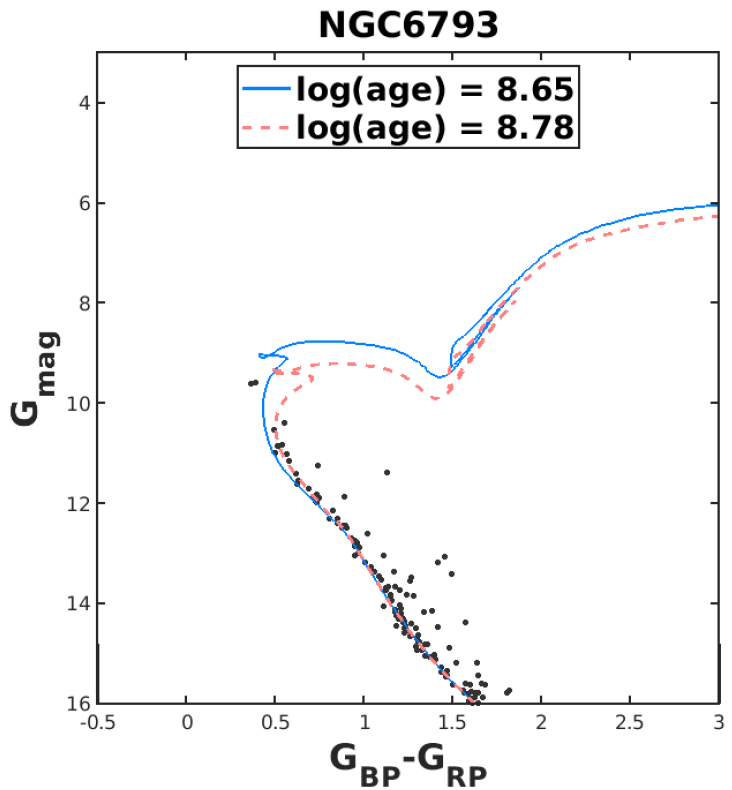
\includegraphics[width=1.0\textwidth]{bossini_ngc6793_different_age_estimate.png}
\caption{Disagreement on Gaia DR2 age estimates for NGC 6793 between GC18 (dashed red line) and \cite{2019A&A...623A.108B} (solid blue line). The reasons for the disagreement are summarised in the main text. Source:\cite{2019A&A...623A.108B}}
\label{bossini_age_cmd}
\end{center}
\end{figure}

\cite{2019A&A...623A.108B} claim that, in the case of NGC 6793 and other clusters, the estimated age values given by GC18 are inaccurate. In some cases the authors ascribe this as being due to the clusters being inconspicuous, while in others, including NGC 6793, they ascribe this to errors made in the membership determination of certain stars. For NGC 6793, they claim that a high-likelihood member at $G \sim\ 9$, as determined by \cite{2018A&A...618A..93C}, is missing from the dataset of cluster members used in GC18 and that this star, if taken to be a member of NGC 6793, causes the position of the MSTO in the cluster to change. The authors calculated that the new MSTO, instead of the GC18 value of log(age) = 8.78 (age = 603 Myr), gives an estimated value of log(age) = 8.65 , or a cluster age of 447 Myr. This indicates that the uncertainty in ages caused by the choice of extinction treatment can be less significant than uncertainty caused by disagreement over cluster membership. Such a disagreement is solely due to member selection criteria and does not impact on the difference between different methods of extinction treatment, which is the focus of this project. \\*

However, the significance of the choice of extinction treatment is not impacted by cluster membership disagreements, as the new age estimate made by \cite{2019A&A...623A.108B} is still subject to the same extinction treatment as that of GC18. As shown in Figure \ref{NGC_6793_isoc_inset_1.1_500_0.062}, in order to align the positions of best-fit isochrones generated using two different extinction treatments, there must be differences in the estimates for the cluster age, $A_{V}$ and metallicity between the two isochrones. Since this result is independent of the position of the isochrones in the CMD, using a new age estimate for a fixed-extinction best-fit isochrone, with no change in the other parameters, simply requires a new estimate for the FBER isochrone, in order to realign the MSTOs in both isochrones again. This is shown in Figure \ref{NGC_6793_bossini}, where the path traced by a fixed-extinction isochrone of 450 Myr, representing the \cite{2019A&A...623A.108B} age estimate for NGC 6793, is only matched by an FBER isochrone of around 350 Myr. For both isochrones, the $A_{V}$ and [Fe/H] values are the same as those found in the GC18 and the final columns, respectively, of Table \ref{NGC6793_result}.\\*

While the two isochrones plotted in Figure \ref{NGC_6793_bossini} do not trace the observation data as accurately as those in Figure \ref{NGC_6793_isoc_inset_1.1_500_0.062}, they have been included here simply to illustrate the conclusion, supported by the isochrones in both figures, that using a different fixed-extinction age estimate does not alter the significance of the effect of using different extinction treatment methods on the estimated cluster properties, which are required to place a given isochrone along a particular path. The disagreement between GC18 and \cite{2019A&A...623A.108B} over the cluster age are merely over the location of the path traced by the best-fitting isochrone for the cluster, arising from the disputed membership of a particular star. \\*

\begin{figure}[h!]
\begin{center}
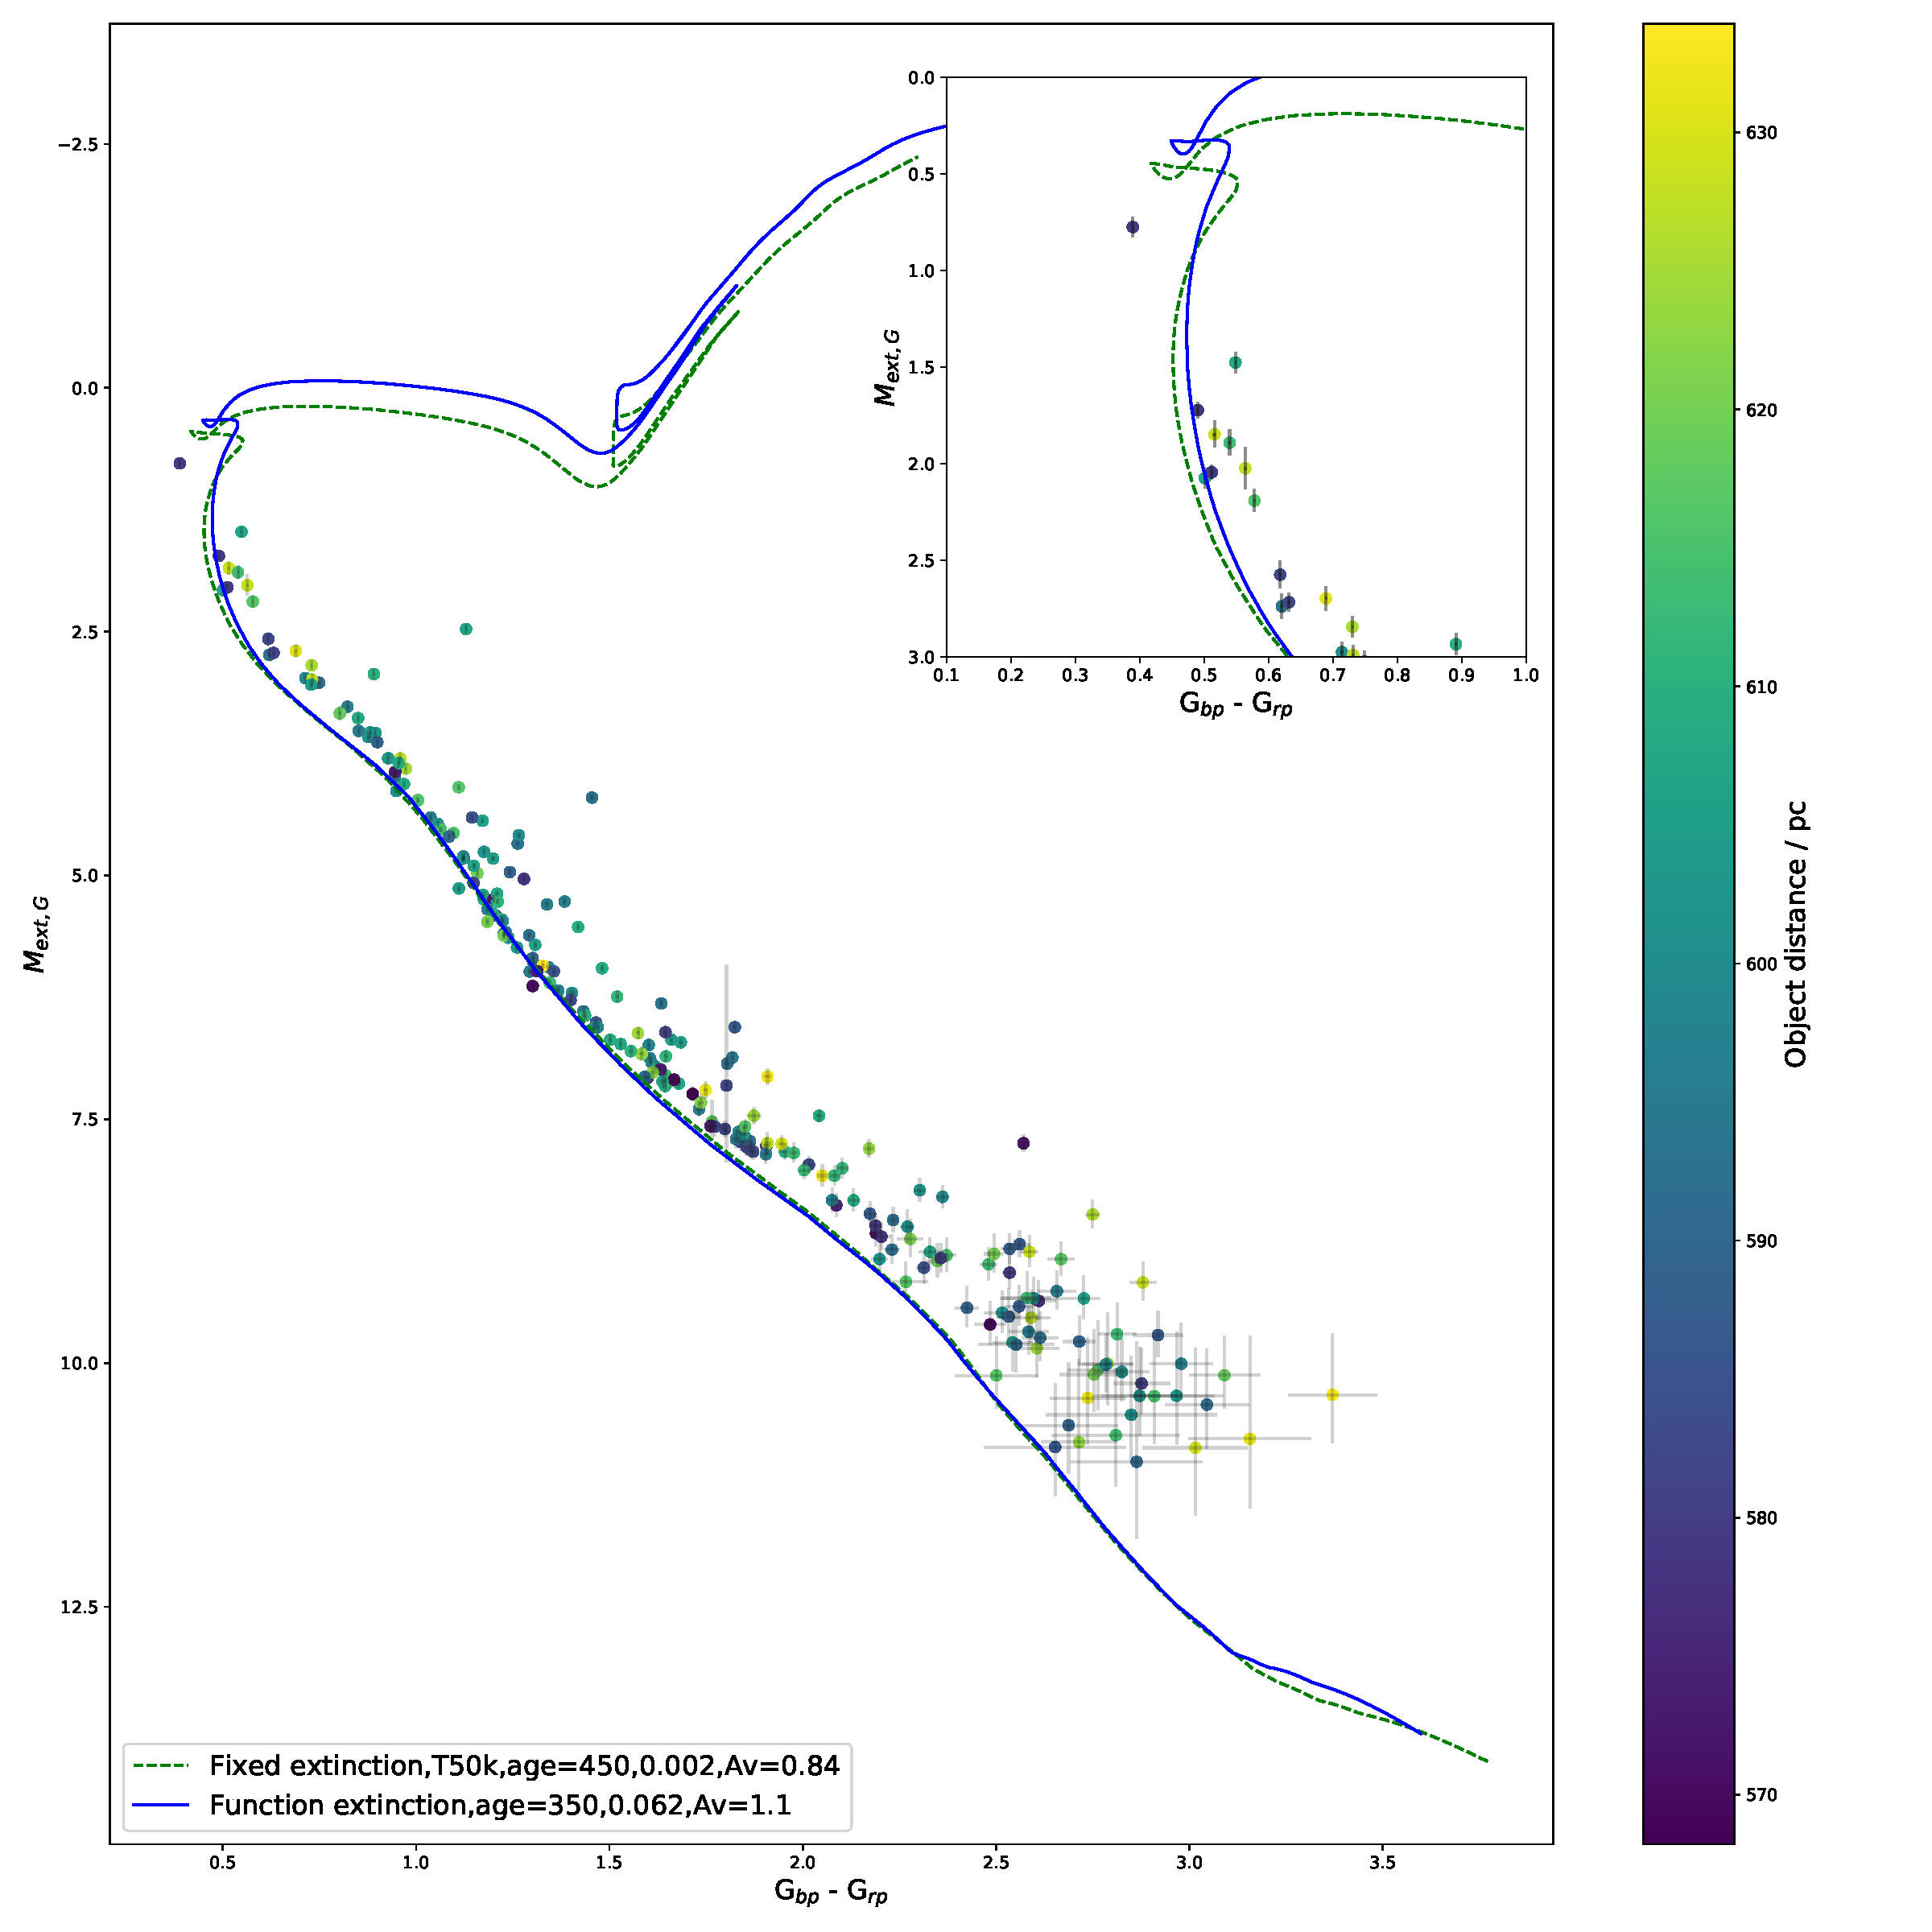
\includegraphics[width=1.0\textwidth]{../NGC_6793_CMD_FeH_0p062_Av_1p1_350Myr_vizier_isochrones_summary_errorbars.pdf}
\caption{Same format as Figure \ref{NGC_6793_isoc_inset_1.1_500_0.062}. The fixed-extinction isochrones for both $(A_{X}/A_{V})_{plat}$ (dashed green line) and $(A_{X}/A_{V})_{MS}$ (dashed red line) have ages of 450 Myr, while the $A_{V}$ and [Fe/H] values are the same as those used for the GC18 isochrones. The FBER isochrone (solid blue) has the same $A_{V}$ and [Fe/H] as listed in the final column of Table \ref{NGC6793_obs} and an age of 350 Myr.}
\label{NGC_6793_bossini}
\end{center}
\end{figure}

\subsubsection{Choice of isochrone software}

The conclusion that different extinction treatment methods produce different cluster parameter estimates could have its validity undermined by a different source of uncertainty. When comparing the best-fit isochrone results of this project for NGC 6793 with those from GC18, this project employs the latest BaSTI isochrone database \citep{2018ApJ...856..125H} for the fixed-extinction treatment, while GC18 uses the PARSEC isochrone database \citep{2017ApJ...835...77M} for the same. This project's use of isochrones generated by a different model stellar evolution code from that used by GC18 could impact the validity of comparing the $A_{V}$ values, ages and metallicities arising from both extinction treatments.\\*

A recent comparison of isochrones, including those generated using BaSTI and PARSEC, was made by \cite{2019MNRAS.483.4949G}. The authors carried out a detailed set of observations of the Galactic globular cluster NGC 5904 in 29 photometric bands. The CMDs created from these data were used to fit isochrones from five different databases, including PARSEC and BaSTI. They adopted the \cite{1989ApJ...345..245C} extinction law with the parameters having values of $R_{V} = 3.60\pm0.05$ and $A_{V} = 0.20\pm0.02$. As shown in Table \ref{NGC5904_obs_gontcharov}, the Gaia colour excess $E(G_{\textnormal{bp}} - G_{\textnormal{rp}})$ for NGC 5904 differs significantly between the best-fits from the two isochrone databases, which in turn causes disagreements for the projected cluster age and (photometric) distance. Across all filter systems and isochrone databases, the authors calculated mean estimates of the cluster properties and found that the resulting photometric distance to be in agreement with the cluster distance calculated from the Gaia parallaxes of the cluster members.\\*

\begin{table}
\begin{center}
\begin{tabular}{ccc}
\hline
Cluster property & PARSEC & BaSTI \\
\hline
$E(G_{\textnormal{bp}} - G_{\textnormal{rp}})$ / mag & 0.080$\pm$0.02 & 0.013$\pm$0.03 \\
Age / Gyr & 11.5 & 12.5 \\
Distance / pc & 7600 & 8400 \\
\hline
\end{tabular}
\caption{Comparison of best-fit parameter results for NGC 5904 using PARSEC and BaSTI. Data taken from \cite{2019MNRAS.483.4949G}.}
\label{NGC5904_obs_gontcharov}
\end{center}
\end{table}

In the case of the analysis of NGC 6793 carried out in this project, the distance measurements are derived from Gaia parallax measurements and so are unaffected by the choice of model stellar evolution code used to generate isochrones, allowing the GC18 cluster distance to be validly assumed here (as 600 pc to the cluster centre). Furthermore, using the PARSEC-derived parameters from GC18, an accurate BaSTI model isochrone for NGC 6793 was calculated successfully for a fixed $A_{X}/A_{V}$ extinction model. Therefore, it was concluded that the validity of comparing the respective $A_{X}$, [Fe/H] and age values from GC18 and this project was not endangered by the use of different isochrone databases by each study.\\*


As predicted by the comparisons made for isochrones in the Gaia CMD in Section \ref{Gaia_isoc}, the FBER isochrone at the GC18 estimated value of $A_{V} = 0.843$ is systematically too blue and too bright to fit to the observed CMD of NGC 6793. This remains the case regardless of changes in age and metallicity. Therefore, as predicted, there is significant disagreement between the best-fitting $A_{V}$ values for the two extinction treatment methods.\\*

\subsubsection{MSTO location}
There are considerable uncertainties for the parameters in both of the isochrones plotted in Figure \ref{NGC_6793_isoc_inset_1.1_500_0.062}. Most fundamentally, the position of the MSTO is reliant only on the position of the handful of stars forming the brightest cluster members. The parallax errors for lower MS stars, as shown in Figure \ref{NGC_6793_obs_only}, are large enough to make the effect of any changes in metallicity for either isochrone insignificant. On the other hand, any significant changes in $A_{V}$ and age cause misalignment of the main sequence and MSTO, respectively, with the observational data.\\*

As demonstrated in \cite{2019A&A...623A.108B}, the selection of the true location of the MSTO in the observational CMD is disputed. Therefore, the possible locations of the MSTO in Figure \ref{NGC_6793_obs_only} are briefly assessed here.\\*

The two objects to the right of the MS which appear to form a straight line connecting to the MS at $M_{\textnormal{ext},G} \approx 3-3.5$ were not considered to represent the location of the MSTO due to the much larger number of blue stragglers than MSTO objects that would result from placing the MSTO there. Furthermore, the shape of the would-be MSTO region does not match the shape of the same region in any isochrone tested on the region. Overall, therefore, the MS region at $M_{\textnormal{ext},G} \approx 3-3.5$ cannot be the MSTO region.\\*

Looking at the CMD number density of member objects along the upper main sequence of NGC 6793, specifically for the region $M_{\textnormal{ext},G} < 5$, it would be expected that main sequence stars at and below the MSTO heavily outnumber any blue stragglers constituting any population of MS-like objects above the MSTO point. Since the number density of stars in the upper MS is relatively uniform until $M_{\textnormal{ext},G} \approx 1.5$, it was considered that regions fainter than this point were unlikely to represent locations above which the number density would markedly decrease, and therefore were unlikely to represent the location of the MSTO and the start of the blue straggler population. This assessment agrees with those made by GC18 and \cite{2019A&A...623A.108B}. Since the observational data used in this project to determined the MSTO location is the same as that used by GC18, but not in \cite{2019A&A...623A.108B}, it was considered that using the same CMD location as GC18 for the MSTO would be advantageous, particularly since any differences in the estimated cluster age between the fixed-extinction and FBER isochrones have been determined using the same CMD location for the MSTO for both isochrones.\\*

\section{Final assessment of results}

In summary, the use of the FBER treatment on isochrones, when applied to the Gaia CMD for NGC 6793, required significant changes in the values of $A_{V}$, metallicity and age for the best-fitting isochrone, compared with those derived by GC18, to align with the observed sample of stars in the cluster (see Table \ref{NGC6793_result} for details). Using the FBER treatment results in an observed sample requiring higher $A_{V}$ extinction, higher metallicity and, most importantly, a younger age in its best-fitting isochrone, compared to the standard fixed-extinction ratio treatment. Furthermore, the best-fit isochrones for both treatments have a similar level of accuracy to the observational data in the CMD.\\*

The use of different stellar isochrone databases in GC18 and this project was found to have no significant impact when comparing the resulting parameter values for the NGC 6793 data provided by GC18. The uncertainties derived from parallax and photometric measurements errors were found to be significant only in the lower MS and therefore created sizeable uncertainties for the optimal cluster metallicity but not for the age or $A_{V}$ value. Uncertainties due to the membership of certain stars or the CMD location of the MSTO does not impact the conclusion that FBER isochrones require significantly different cluster parameters than fixed-extinction isochrones in order to align with a given observational dataset. The uncertainties caused by the errors in the coefficients of the FBER models are not sufficiently large to undermine this conclusion.\\*

Of particular interest is the difference in estimated cluster ages for NGC 6793, for the MSTO locations given in both GC18 and \citep{2019A&A...623A.108B}. This is important because this project has shown in Section \ref{result_CMDs} that it occurs in multiple CMDs and for different instruments, so there is the potential for this difference to occur for a large number of observations for different star clusters. If this apparent age discrepancy is found to occur for a significantly large number of star clusters, it could potentially cause a revision of the history of star clusters and, subsequently, their host galaxies. \\*

\chapter{Conclusion}
This project aimed to use theoretical stellar atmosphere data to map variations in the extinction ratios $A_{X}/A_{V}$ in three different photometric filter systems as the atmospheric effective temperature, surface gravity and metallicity were varied. The greatest variations in $A_{X}/A_{V}$ for all filters were found to occur with variations in effective temperature, with variations due to changes in metallicity and surface gravity found to be much smaller, as expected. Within individual filters, the greatest mean $A_{X}/A_{V}$ values occurred for UV filters, with the mean $A_{X}/A_{V}$ values decreasing with increasing filter wavelength, again in line with previous predictions and observational evidence. Mathematical functions were constructed and their coefficients fitted to the $A_{X}/A_{V}$ data in each filter. The resulting functions were able to describe the data to a reasonable degree of accuracy, and are therefore a suitable, and much simpler, substitute for performing interpolation on tables of $A_{X}/A_{V}$ data. \\* 

The $A_{X}/A_{V}$ values generated by applying these functions to objects in an isochrone were then added to those objects (the FBER method). The isochrone was then plotted in selected CMDs alongside the same isochrone to which a fixed value of $A_{X}/A_{V}$ was applied to all objects. This allowed the effects of the FBER and fixed extinction ratio methods on the isochrone position in the CMD to be compared. \\*

In all the CMDs studied in this project, applying a fixed value of $A_{X}/A_{V}$ to the entire isochrone causes the main-sequence turn-off to occur at a more luminous, bluer point in a given CMD than the MSTO point for the same isochrone with extinction values derived using the FBER method. The significance of this position change is dependent on the filters used to construct the particular CMD in question. The position changes in two of the four CMDs studied are insignificant.\\*

The WFC3 F814W-(F275W-F814W) CMD shows significant differences between the positions of certain sections of isochrones treated under different extinction-calculation methods, particularly for the lower main sequence but also for the MSTO, depending on the value of $A_{X}/A_{V}$ used in the fixed-extinction case. This is a consequence of the much larger variation of extinction between different stellar types in the UV spectral range.\\*

The Gaia photometric CMD is highly sensitive to both the choice of extinction-calculation method and the choice between $(A_{X}/A_{V})_{plat}$ and $(A_{X}/A_{V})_{MS}$ for the fixed-extinction ratio method. This underscores the substantial risk of incorrect assumptions being made when fitting isochrones to observational data with a single globally-fixed $A_{X}/A_{V}$ value across all constituent stellar model objects, which in turn leads to incorrect estimates of important cluster parameters, as was demonstrated in detail here for the open cluster NGC 6793. \\*

\section{Future work}
There are multiple ways to extend the applicability of the work done in this project. The most obvious examples are to study more CMDs in the filter systems used in this project and to utilise the filter response functions for more filter systems, particularly for more modern and more sensitive instruments, such as the James Webb Space Telescope (JWST) and the proposed WFIRST and PLATO space telescopes, to create FBER models for observations made with these instruments.\\*

Another extension would be to apply the FBER method to observed clusters with isochrone ages previously determined using the fixed-extinction ratio method. If, as predicted for the limited examples studied in this project, the isochrone ages of a given cluster CMD are greater when employing a fixed-extinction method, there is the possibility of a systematic decrease in the predicted ages of these observed clusters after comparison with ages derived using an FBER method.\\*

Regarding the case of NGC 6793, follow-up observations with Johnson-Cousins filters, if feasible, could resolve the $A_{V}$ disagreement between the extinction-calculation methods by providing a direct measured value upon which the Gaia extinction ratios can be calculated.\\*

Finally, the limits on the accuracy of the model functions presented here require investigation, particularly the accuracy limit at the lowest $T_{\textnormal{eff}}$ values available from ATLAS9. This could be done using the same approach as that used by \cite{2008PASP..120..583G}, who use SEDs generated from sources other than ATLAS9 to extend their bolometric correction database to a minimum $T_{\textnormal{eff}}$ of $\sim$1000 K. The coolest known stellar objects (excluding brown dwarfs) have $T_{\textnormal{eff}} \sim 2500$ K. Extending the dataset would constrain the allowed behaviour of the model functions for the lowest ATLAS9 effective temperatures. The lack of data for atmospheres below 3500 K for the ATLAS9 grid used in this project prevents investigation of the significance of the tail-flick phenomenon, since the phenomenon, at present, extends to (and possibly beyond) the lower $T_{\textnormal{eff}}$ limit for the affected filters in ATLAS9.\\*

%\bibliographystyle{ieeetr}
\bibliographystyle{mnras} % unsrtnat
\bibliography{mphil_thesis}

\end{document}